%    \subsubsection{3D Modeling}
%    \label{subsubsec:Modeling}
%    %% description of things modeled in blender for use in the experiment
%    %    \subsubsection{3D Modeling}
%    \label{subsubsec:Modeling}
%    %% description of things modeled in blender for use in the experiment
%    %    \subsubsection{3D Modeling}
%    \label{subsubsec:Modeling}
%    %% description of things modeled in blender for use in the experiment
%    %    \subsubsection{3D Modeling}
%    \label{subsubsec:Modeling}
%    %% description of things modeled in blender for use in the experiment
%    \input{Text/3DModeling}

Ensuring a high level of realism is paramount in Virtual Reality simulation, particularly when aiming to replicate a genuine experience.
In the context of this research, our objective is to assess the reactions of individuals within a building adorned with facades of varying complexity.
Therefore, the precision of our 3D modeling is of utmost significance.

For this purpose, the ``3D modeling'' module realized in Blender (v3.6), serves as the first component and is responsible for generating the 3D models central to our research that include the site and building as a virtual environment where the experiment will be conducted and generating the distinctive facade variations.

The virtual environment created is an exact replica of the Architectural Environment Research Building, also known as Building HE20, which houses our laboratory on the Itoshima campus of Kyushu University (see Figure\ref{fig:RealVs3dModel}).

    %% Figure of Real building next to 3D modeled building
     \begin{figure}[t]
          \centering
          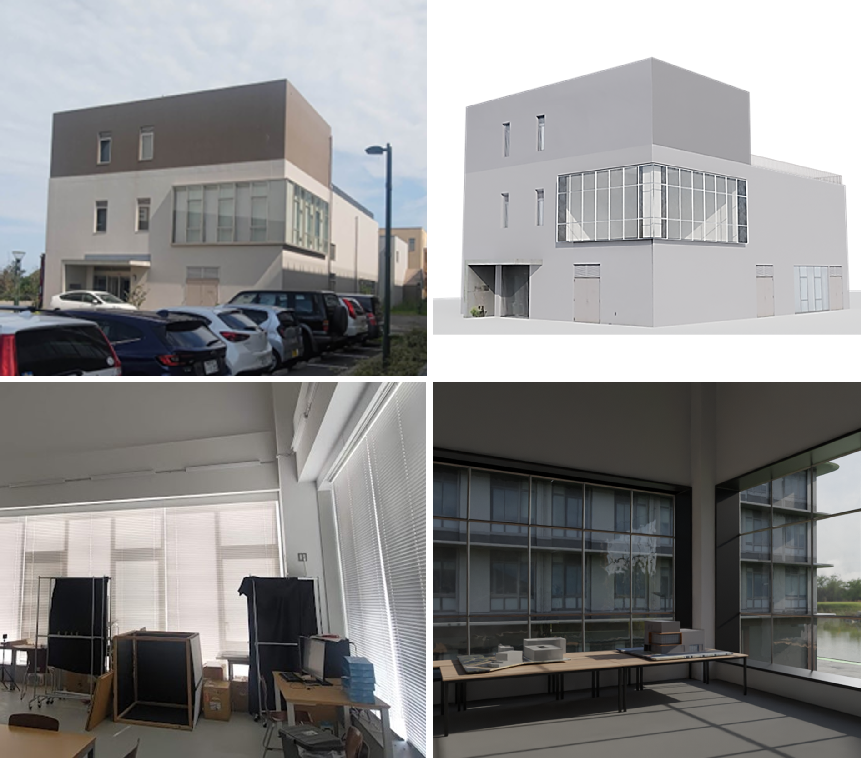
\includegraphics[width= \linewidth]{Images/Realvs3DmodelBlender}
          \caption{Side-by-side comparison of the Architectural Environment Building at Kyushu University used in the experiment, featuring actual interior and exterior photographs (left), and its virtual clone meticulously modeled and rendered in Blender (v3.6) for the Facade Design Complexity Analysis experiment.}
          \label{fig:RealVs3dModel}
        \end{figure}

To ensure an authentic experience, both the exterior of the building and the interior laboratory spaces were meticulously modeled to match the real-world dimensions.
This meticulous approach allows participants to seamlessly navigate the laboratory and revisit their initial encounters with the building's actual conditions, providing a basis for comparison with the virtual simulations.

With the building and its context successfully simulated, the next step was to establish a systematic workflow for creating facade variations with varying degrees of complexity (\ref{tab:PatternsVariationsPart0}).
Our first task was to identify the specific area of the building where the facade variations would be applied.
In Figure\ref{fig:RealVs3dModel}, you can observe that the laboratory's exterior walls feature two sizable windows facing the front and side of the building.
Remarkably, these windows align precisely with our laboratory space, granting an expansive view of a significant portion of the building's facade from inside the lab.

These large glazed surfaces became the central focus for simulating the facade variations.
They offer a unique opportunity for occupants of the laboratory to experience the facade changes firsthand, creating the sensation of being enveloped by the facade variations.
This approach ensures that participants in the experiment perceive a meaningful impact when the facades change from the interior of the lab, a perspective that would typically only be observed from a distance outside the building.

Once the area for applying the facade variations was identified, consisting of the two prominent windows with glazed curtain walls in the lab, the subsequent step was to extrapolate its base mesh and dimensions.
This formed the starting point for delineating the boundaries of the forthcoming building variations.

To enhance the experiment's diversity and variability in modeling facade variations, we chose to commence with three fundamental base patterns, as illustrated in Table\ref{tab:PatternsVariationsPart0} under the `Base Module' row.
These patterns drew inspiration from traditional Japanese motifs and served as the building blocks for creating ten distinct variations within each pattern, ensuring a comprehensive exploration of facade complexity in our study.

The generation of the ten facade variations involves a systematic process that incrementally accumulates complexity.
This progression from level 1 to level 10 is depicted in Table \ref{tab:PatternsVariationsPart0} under the 'Mesh per complexity level' column and is outlined as follows:

Levels 1 to 3: The base mesh is subdivided, creating smaller modules and increasing the pattern density on the facades.

Level 4: The subdivided mesh from level 3 undergoes a one-axis rotation, resulting in a tilted facade.

Level 5: The tilted facade is further bent along its central horizontal axis, forming a concave mesh.

Level 6: Curvature is applied alternately along the vertical axis, producing a wavy mesh.

Level 7: The previously waved mesh is vertically stretched at alternating points, resulting in variations in module size and spacing.

From Level 8 to Level 10: A decimation process is applied to the uniform mesh.
This process disrupts the uniformity of the mesh with minimal overall shape changes\cite{Blender2023}, achieved by collapsing edges.
This reduces the module count while increasing the randomness of the shape and orientation of the base pattern module, creating more complex and varied pattern configurations.

The decimation process is tuned with a \(20\%\) decimation rate for Level 8, \(40\%\) for level 9 and \(60\%\) for level 10.

Finally, the `3d modeling' component' is capable of generating renderings of each facade variation iteration for all three patterns chosen in this research to serve as input for the `Computational Image Complexity Analysis' (CICA) system.
These renderings serve a crucial role in verifying the complexity levels and establishing the ranking of complexity that will guide participants during the experiment.
By visually representing the facade variations, we ensure that the CICA system has the necessary data to evaluate and score the complexity of each iteration accurately.

With a comprehensive understanding of how the 3D modeling component supports the VR system, let's now delve into the application of the CICA system for ranking the 3D-modeled facades.
This process is integral to our Virtual Reality (VR) experiment, where participants will engage with facades featuring various complexity levels.



%
%To represent common challenges in site layout design, we selected three simulated sites (Table \ref{tab:SiteParametersAndPreview}), which included variations in slopes, gradients, and the need to preserve natural features. While these sites were fictitious, they were modeled based on the geographical properties of Fukuoka, Japan, where the experiment was conducted.
%
%The building in the simulation was designed to be photo-realistic (Figure \ref{fig:BuidlingSiteBlenderSimulation}) and served as a focal point for users to explore different positions on the terrain. The "optimization algorithm" of this system (see Figure \ref{fig:MOO_Flowchart}) extracted the building's dimensions, particularly its boundaries, to use them as input to define the building footprint and calculate its impact on the site during the Site Layout Planning process (Table \ref{tab:BuildingParameters}).

    %%Table: Pattern Variations sample 3, 6, 9
    \begin{table*}[htb]
        \centering
        \small
        \caption{Patterns variations for the First five levels of complexity}
        \label{tab:PatternsVariationsPart0}
        \begin{tabularx}
        {\textwidth}{p{4cm} >{\centering\arraybackslash}X >{\centering\arraybackslash}X >{\centering\arraybackslash}X }
            \toprule
            \textit{Description} &
              \textit{Pattern 1} &
              \textit{Pattern 2} &
              \textit{Pattern 3} \\
            \midrule
            \text{Pattern Name} & Hishi Pattern & Tortoise shells & Asanoha Pattern\\

            \midrule
            \textit{Base Module} &  &  &
            \\
            {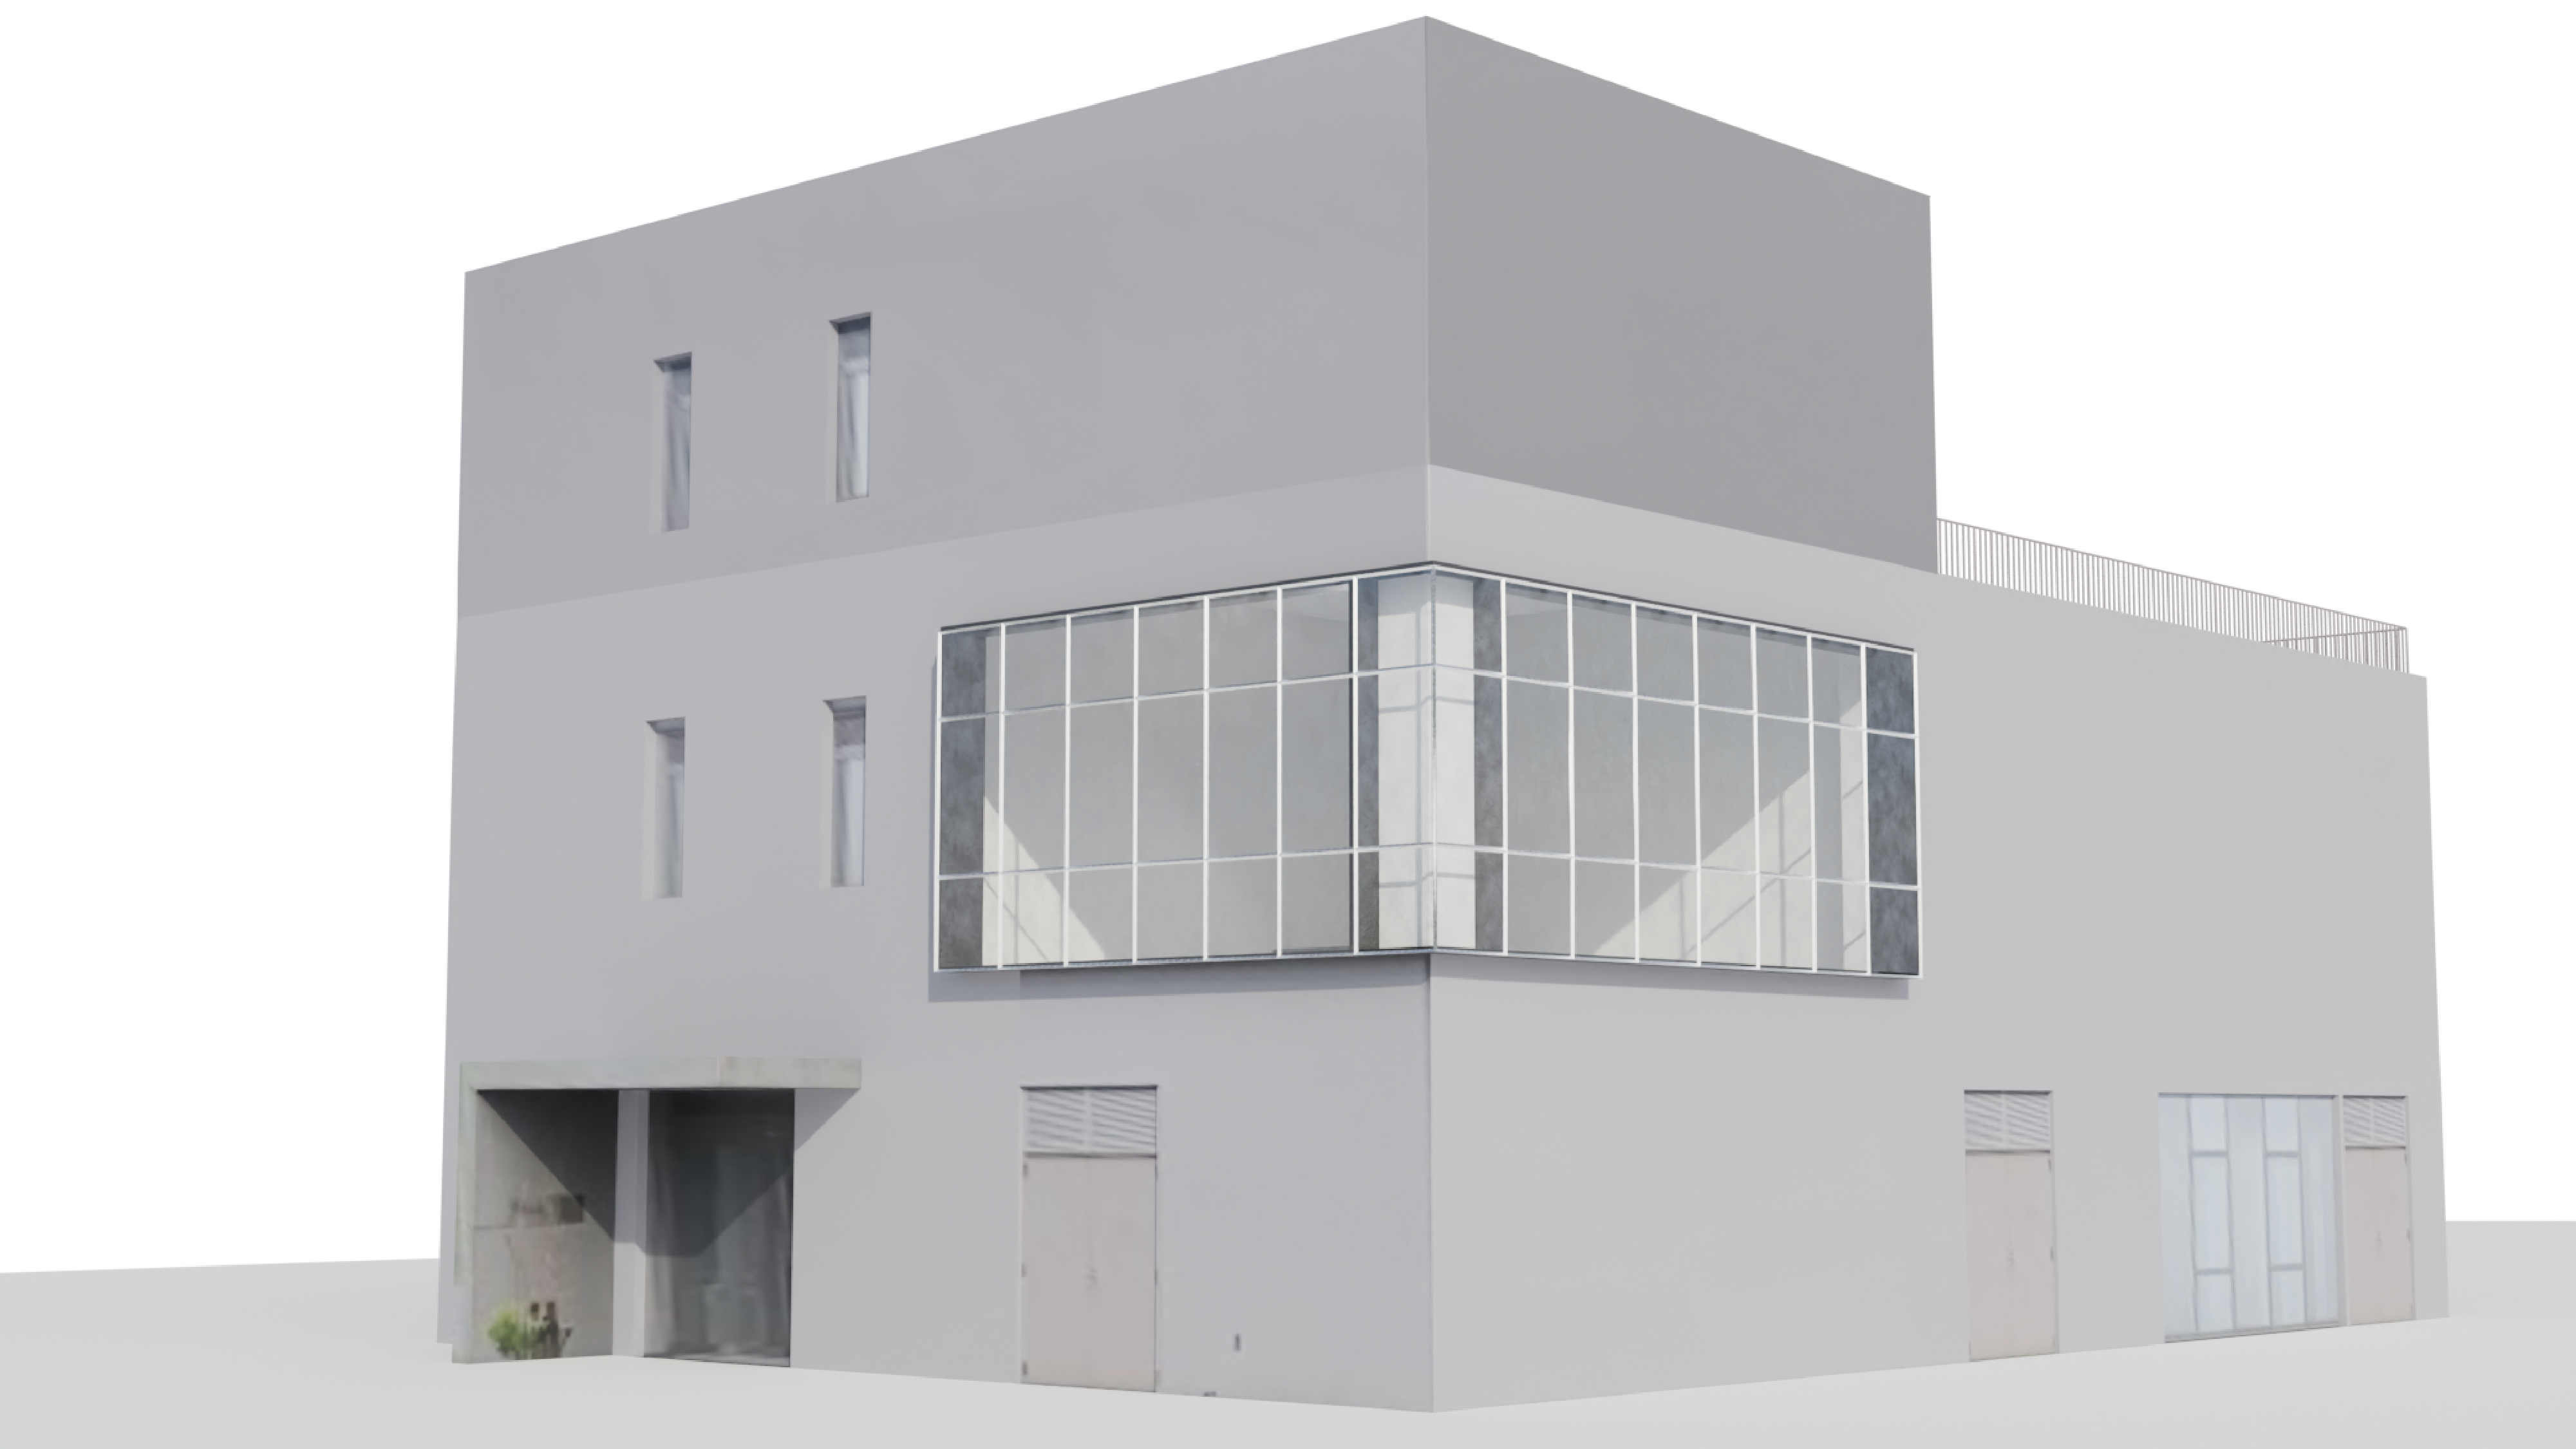
\includegraphics[width=1\linewidth]{Images/Base Module/Building}} &
              {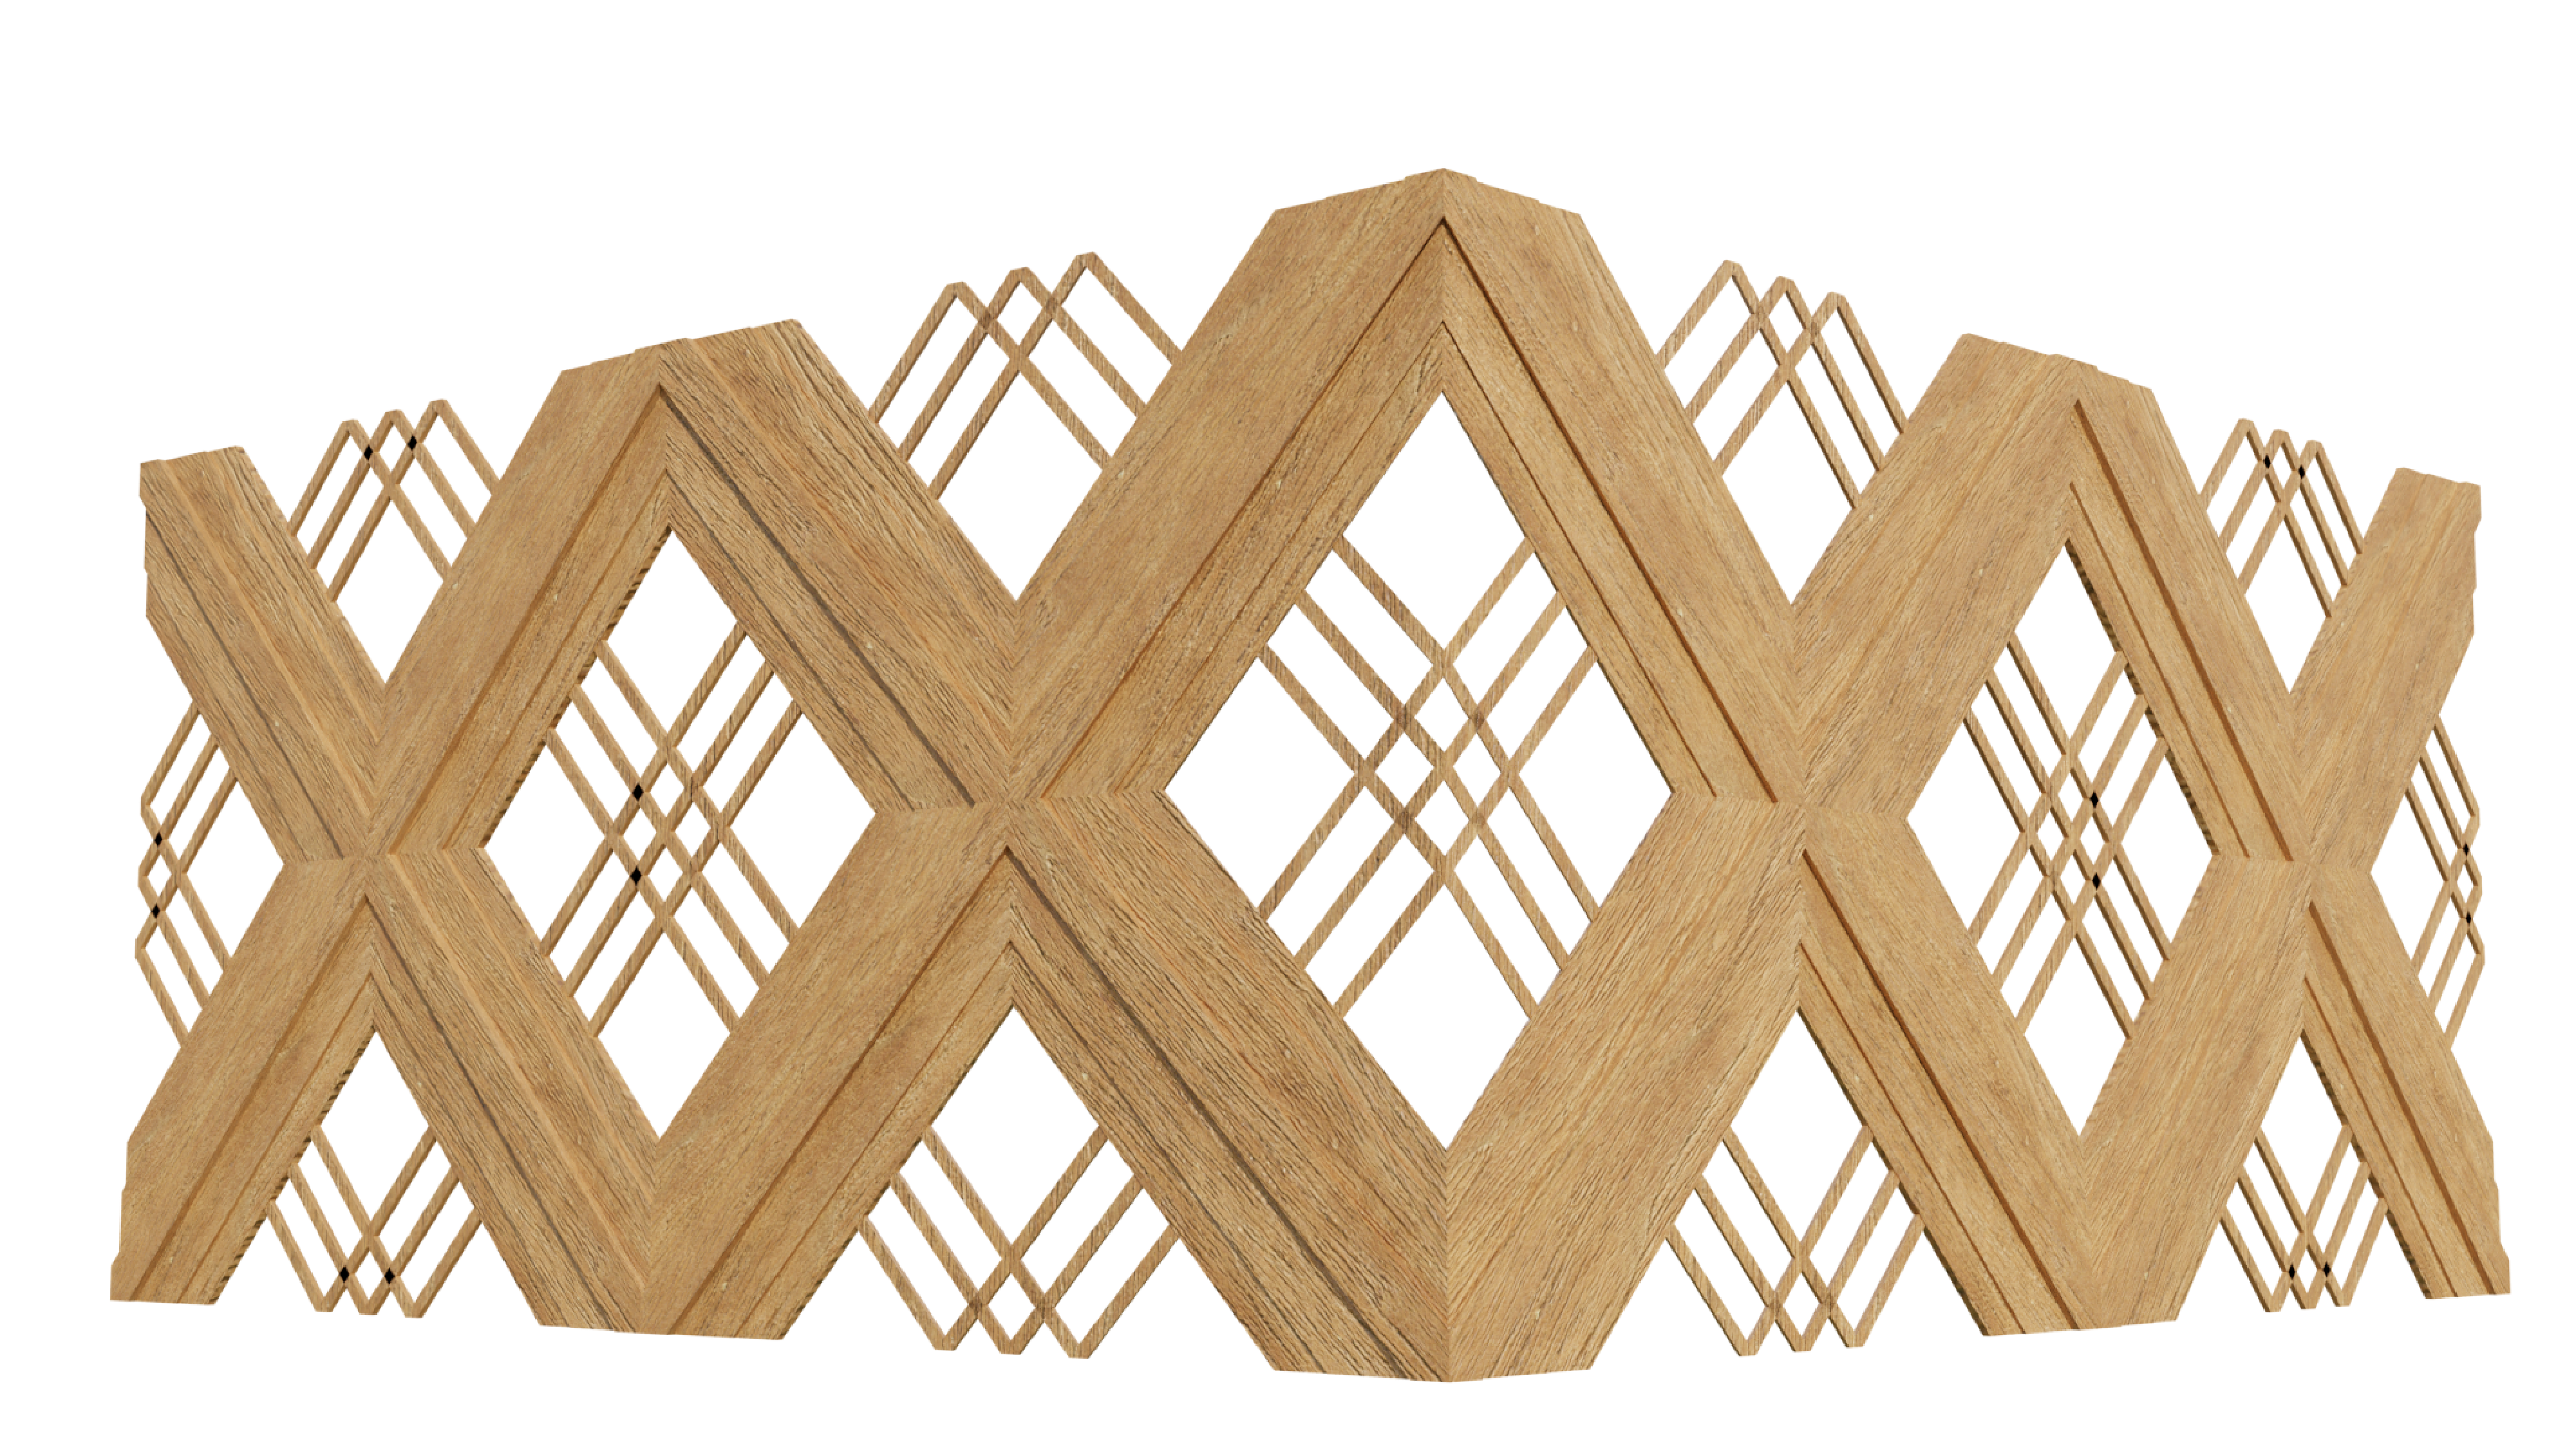
\includegraphics[width=1\linewidth]{Images/Base Module/Pattern1}} &
              {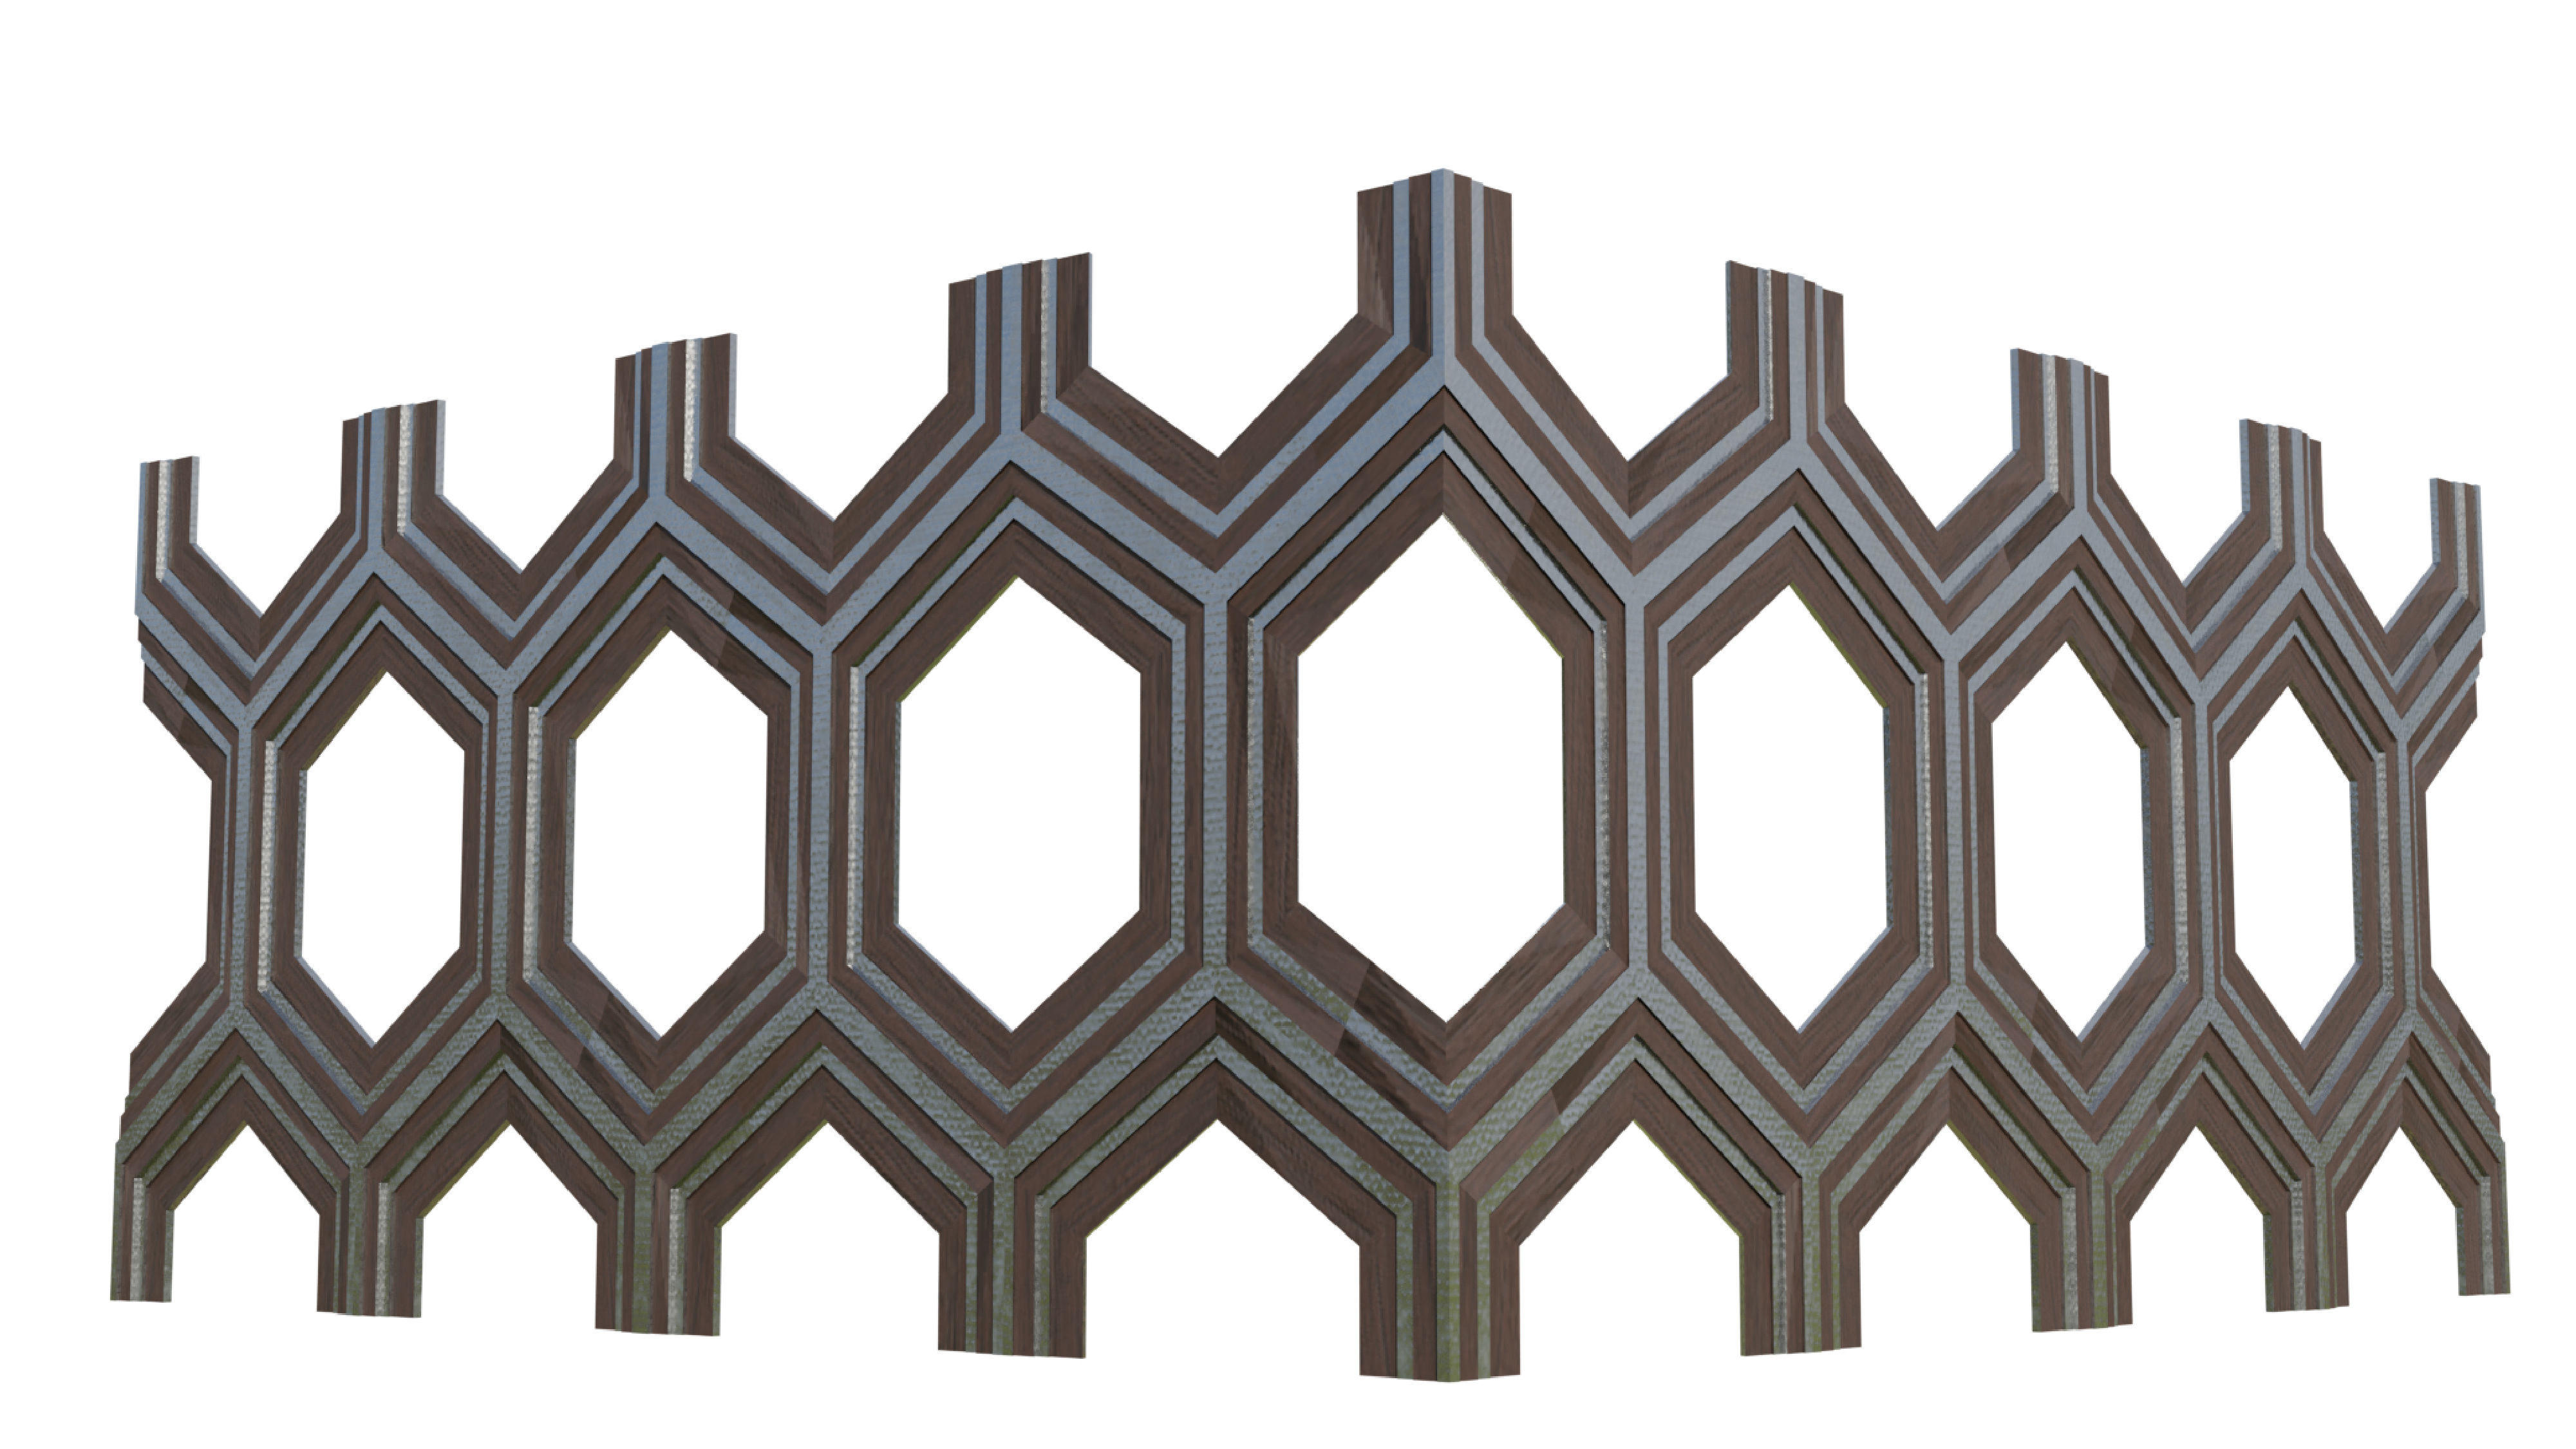
\includegraphics[width=1\linewidth]{Images/Base Module/Pattern2}} &
              {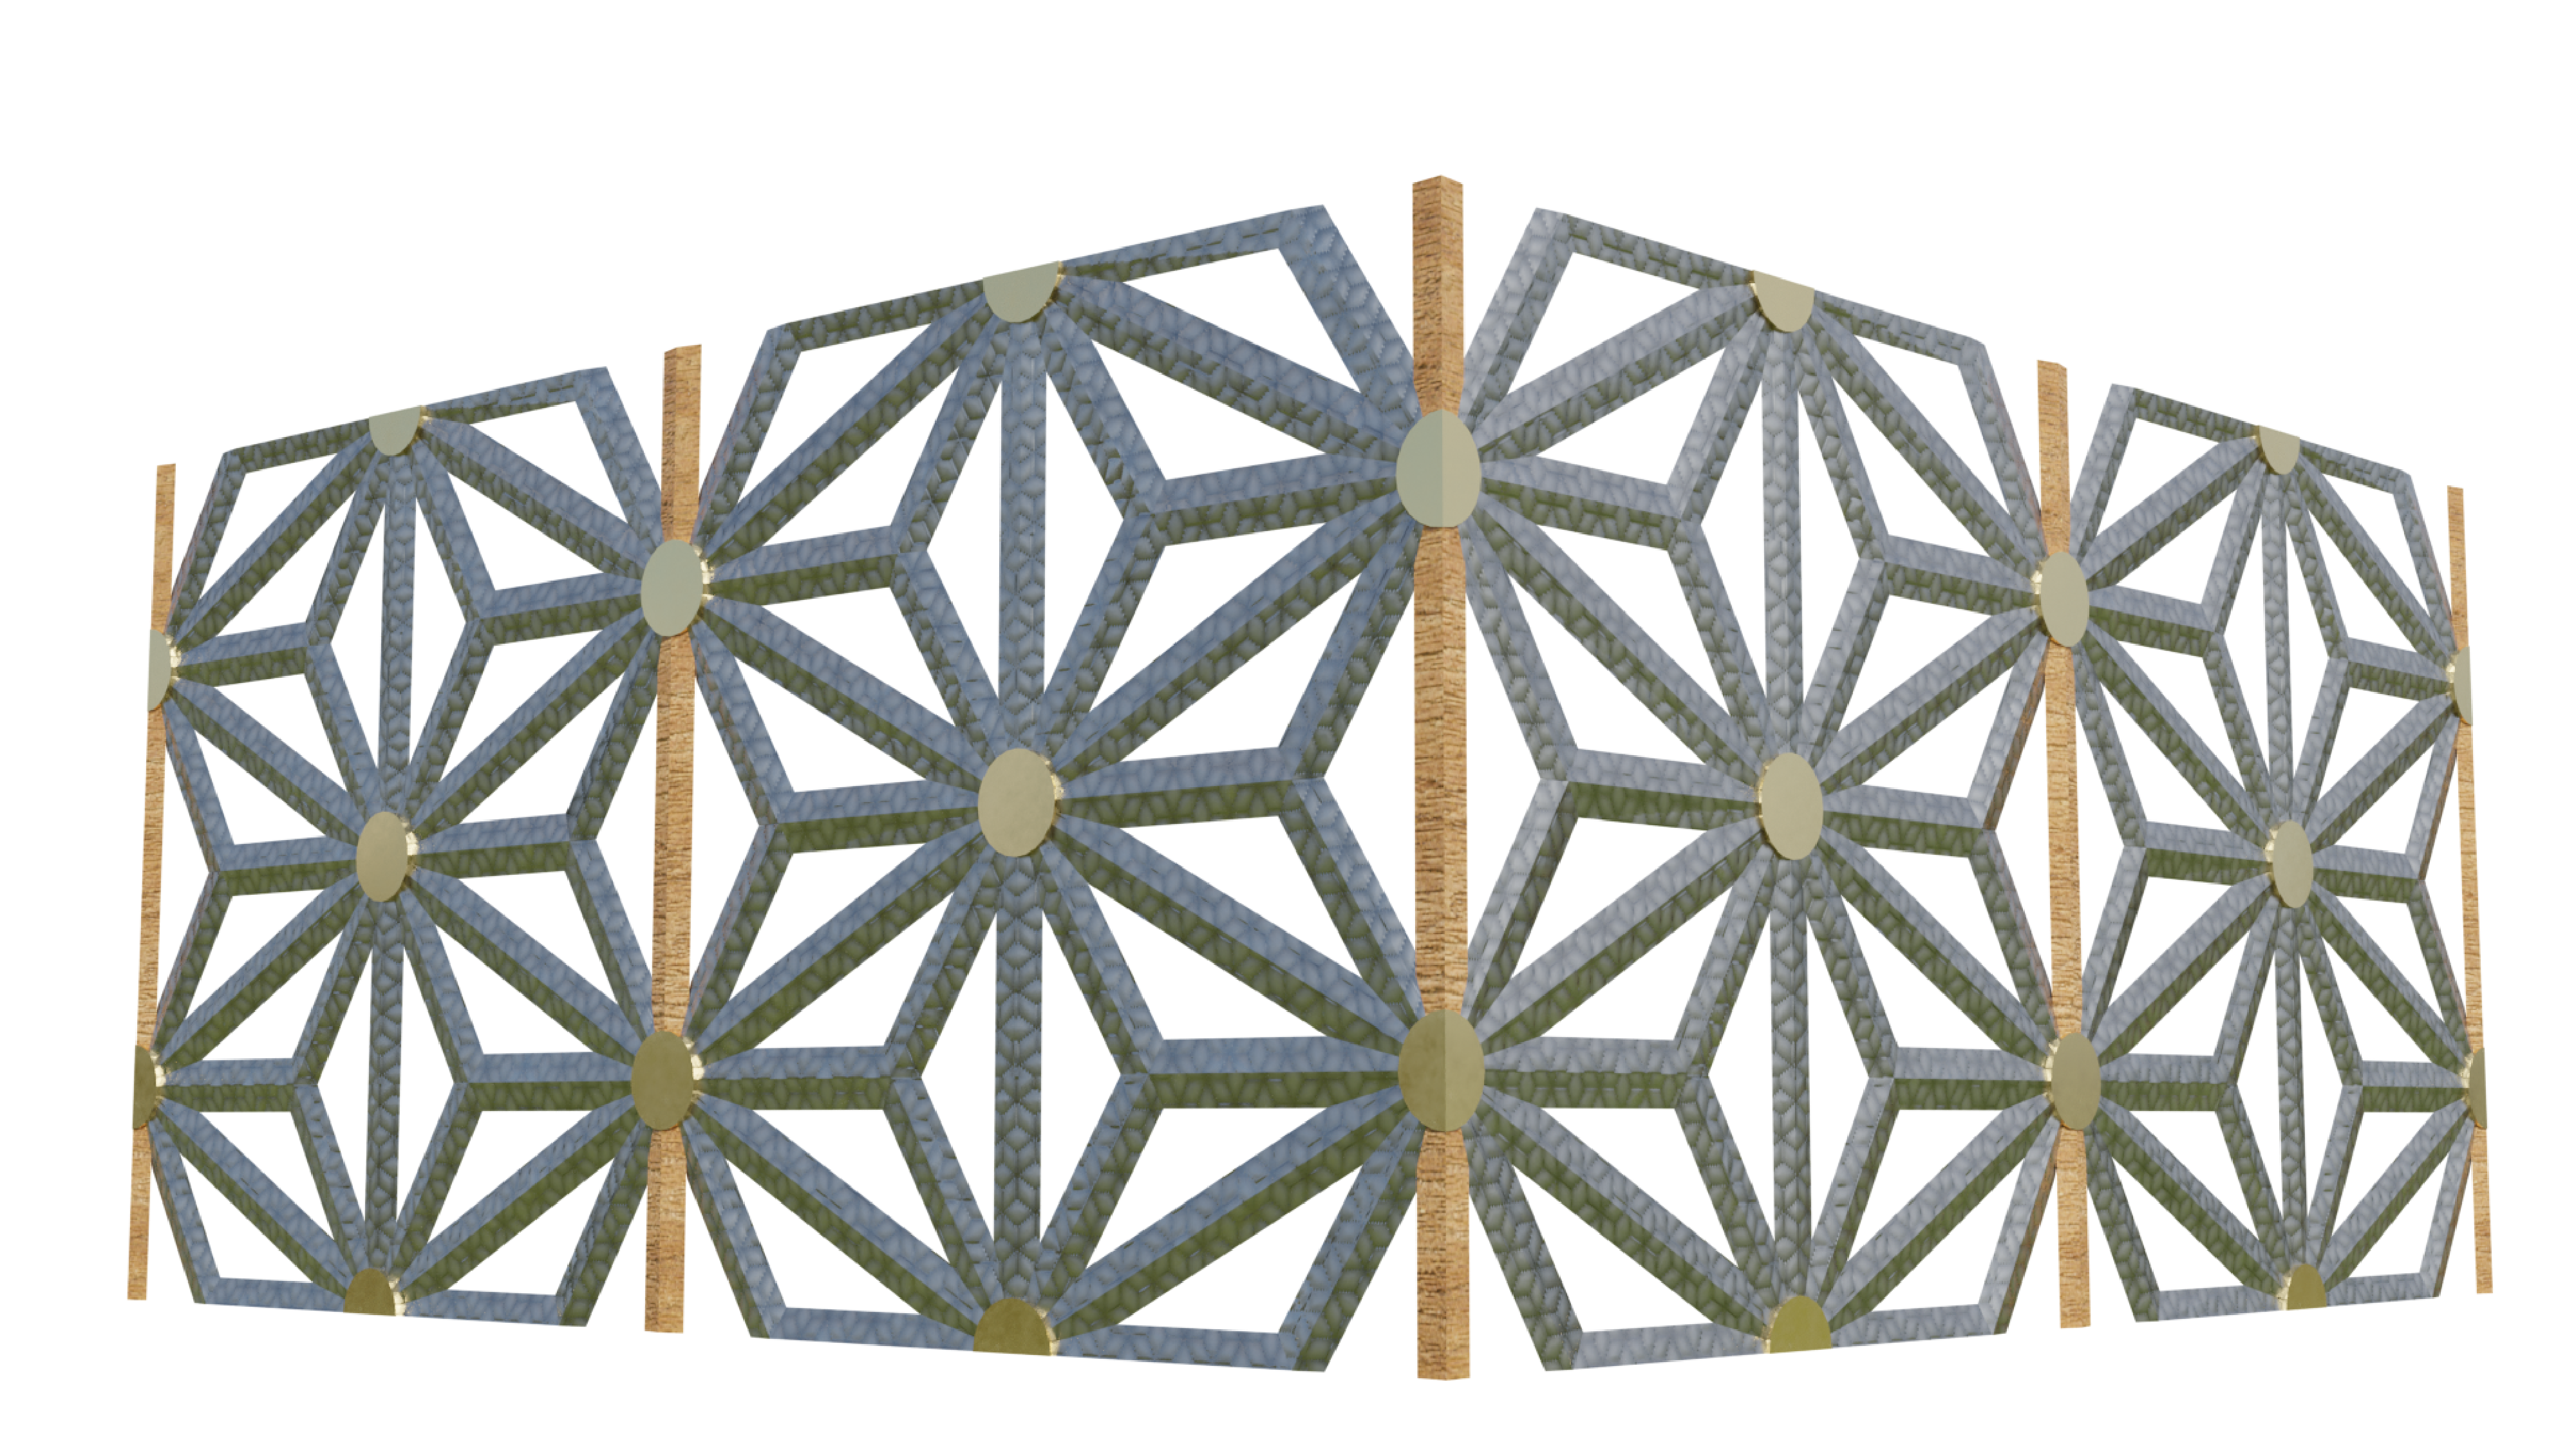
\includegraphics[width=1\linewidth]{Images/Base Module/Pattern3}} \\

            \midrule
            \textit{Mesh per complexity Level} &
              \textit{Pattern 1} &
              \textit{Pattern 2} &
              \textit{Pattern 3}\\

            \midrule
            \text{Level 3} &  &  &
            \\
            {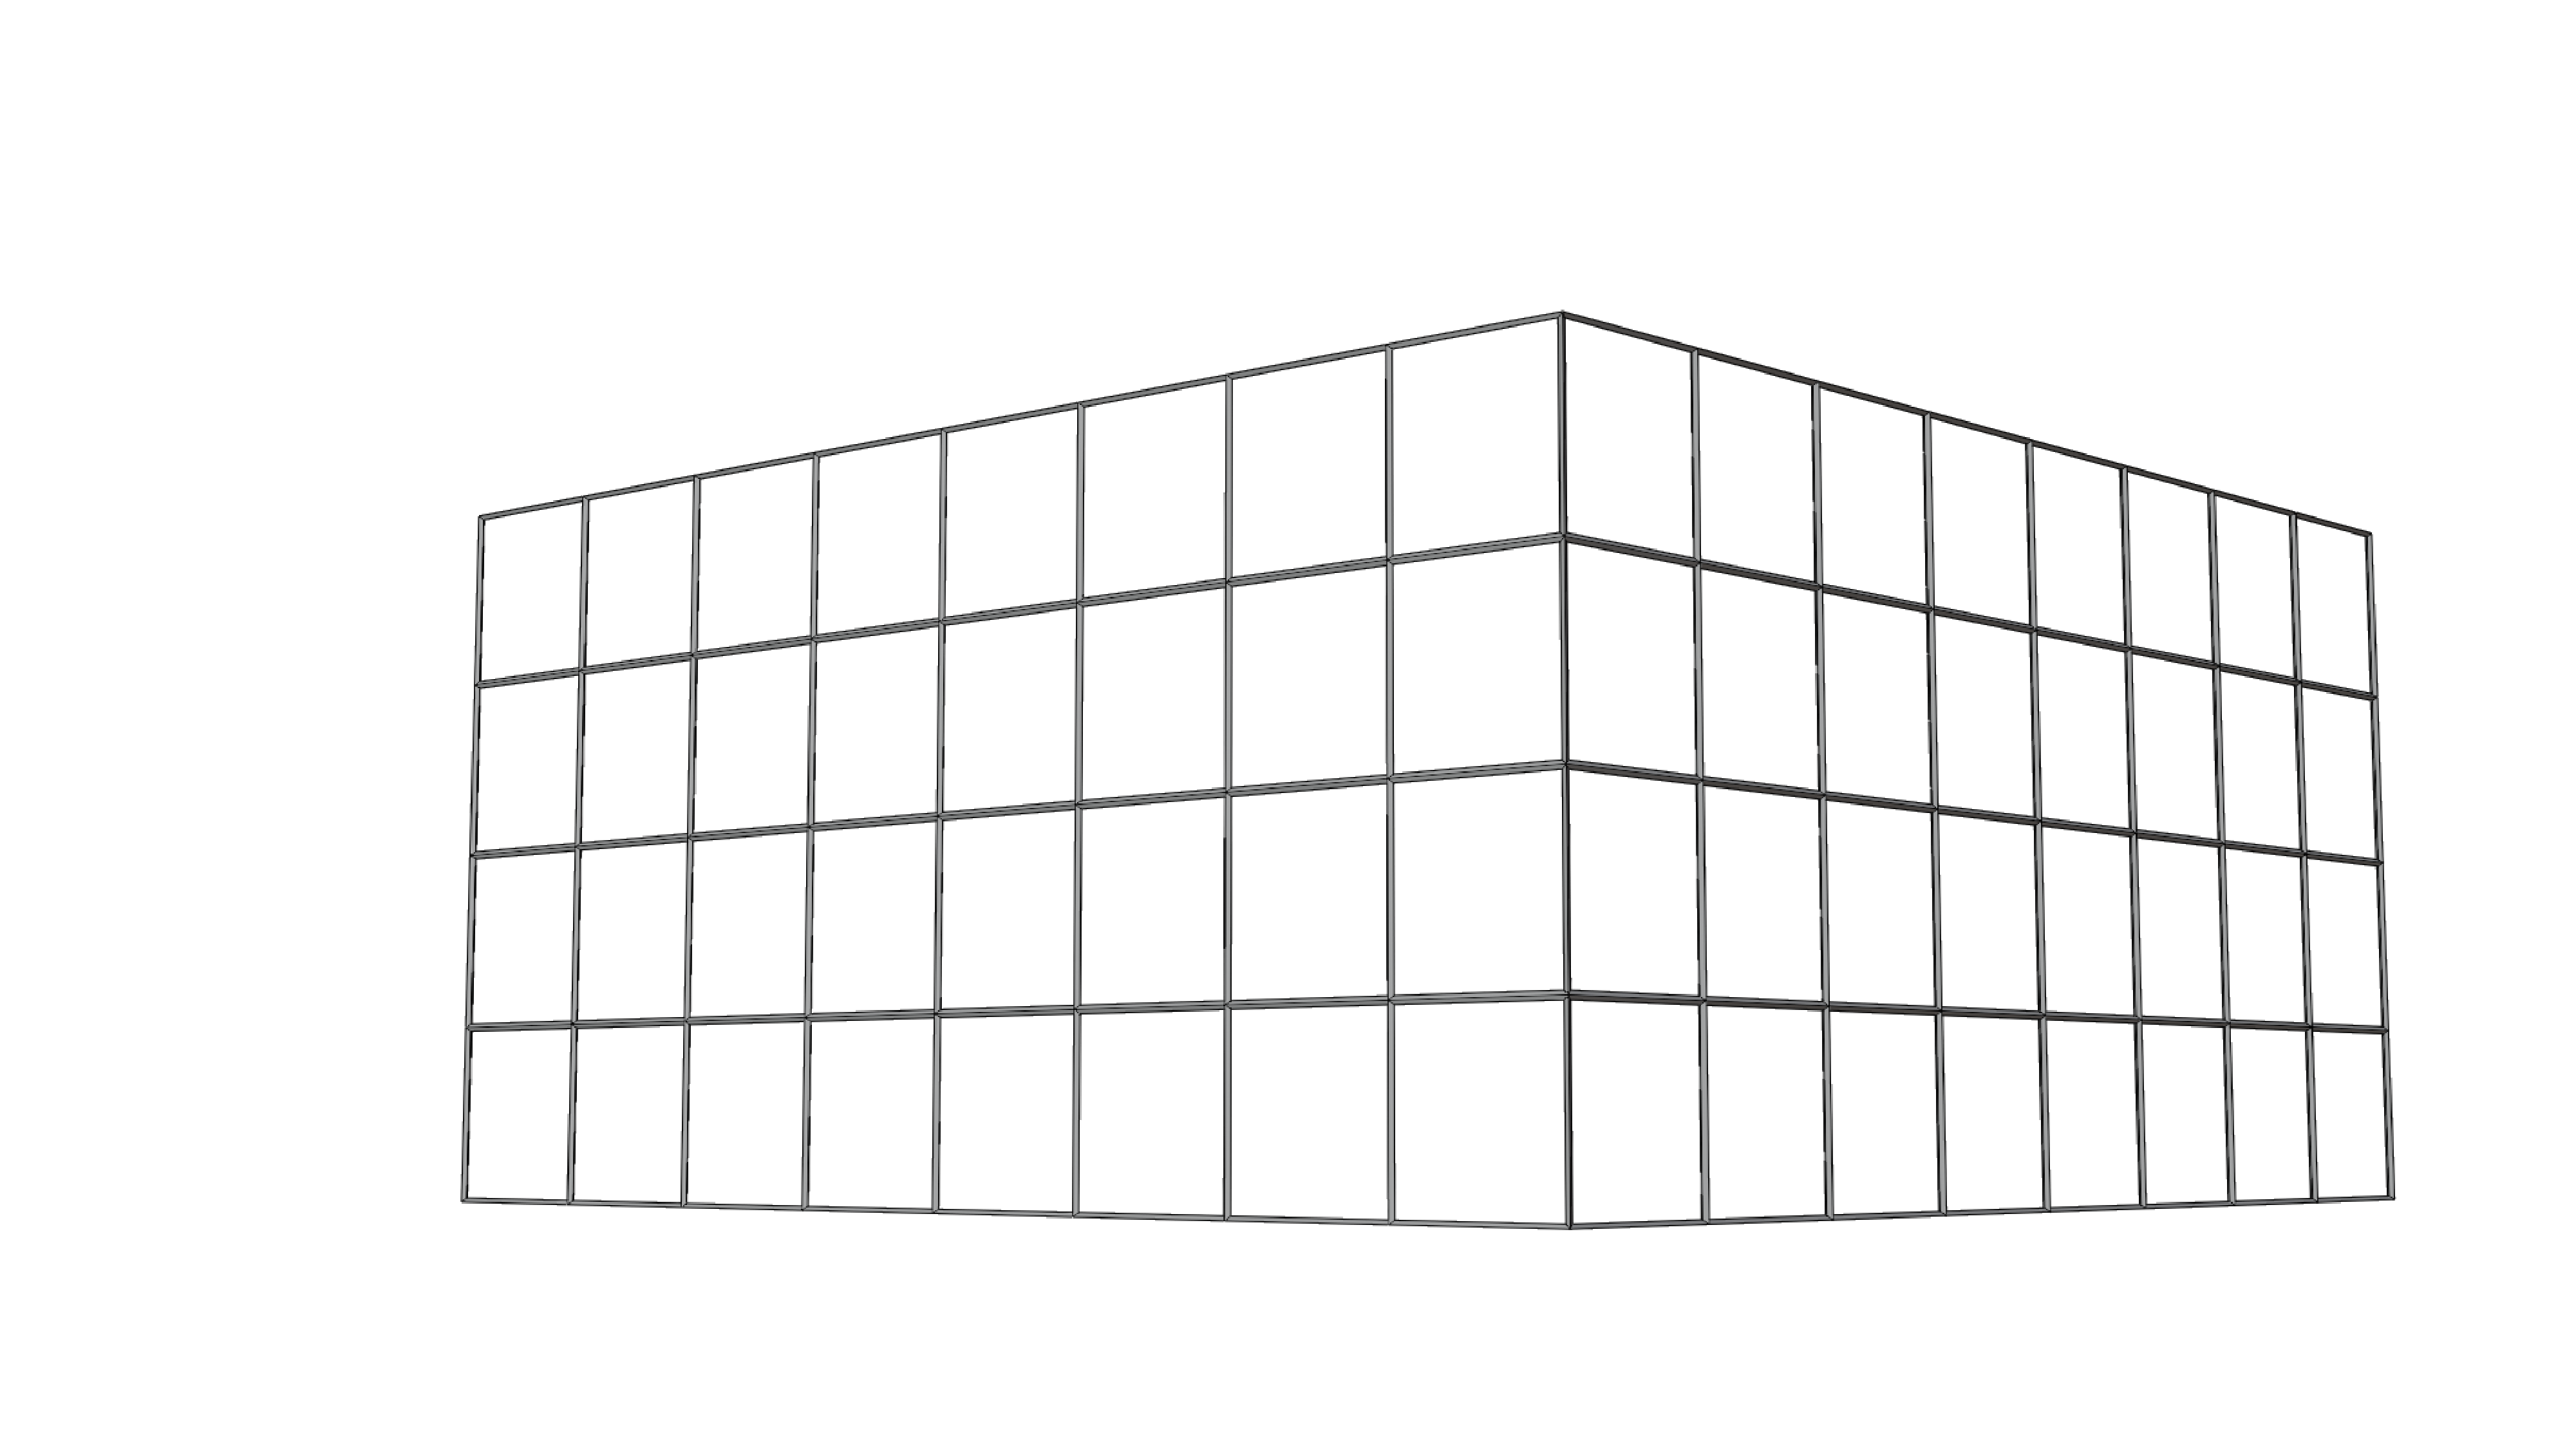
\includegraphics[width=1\linewidth]{Images/Wall 0/0003}} &
              {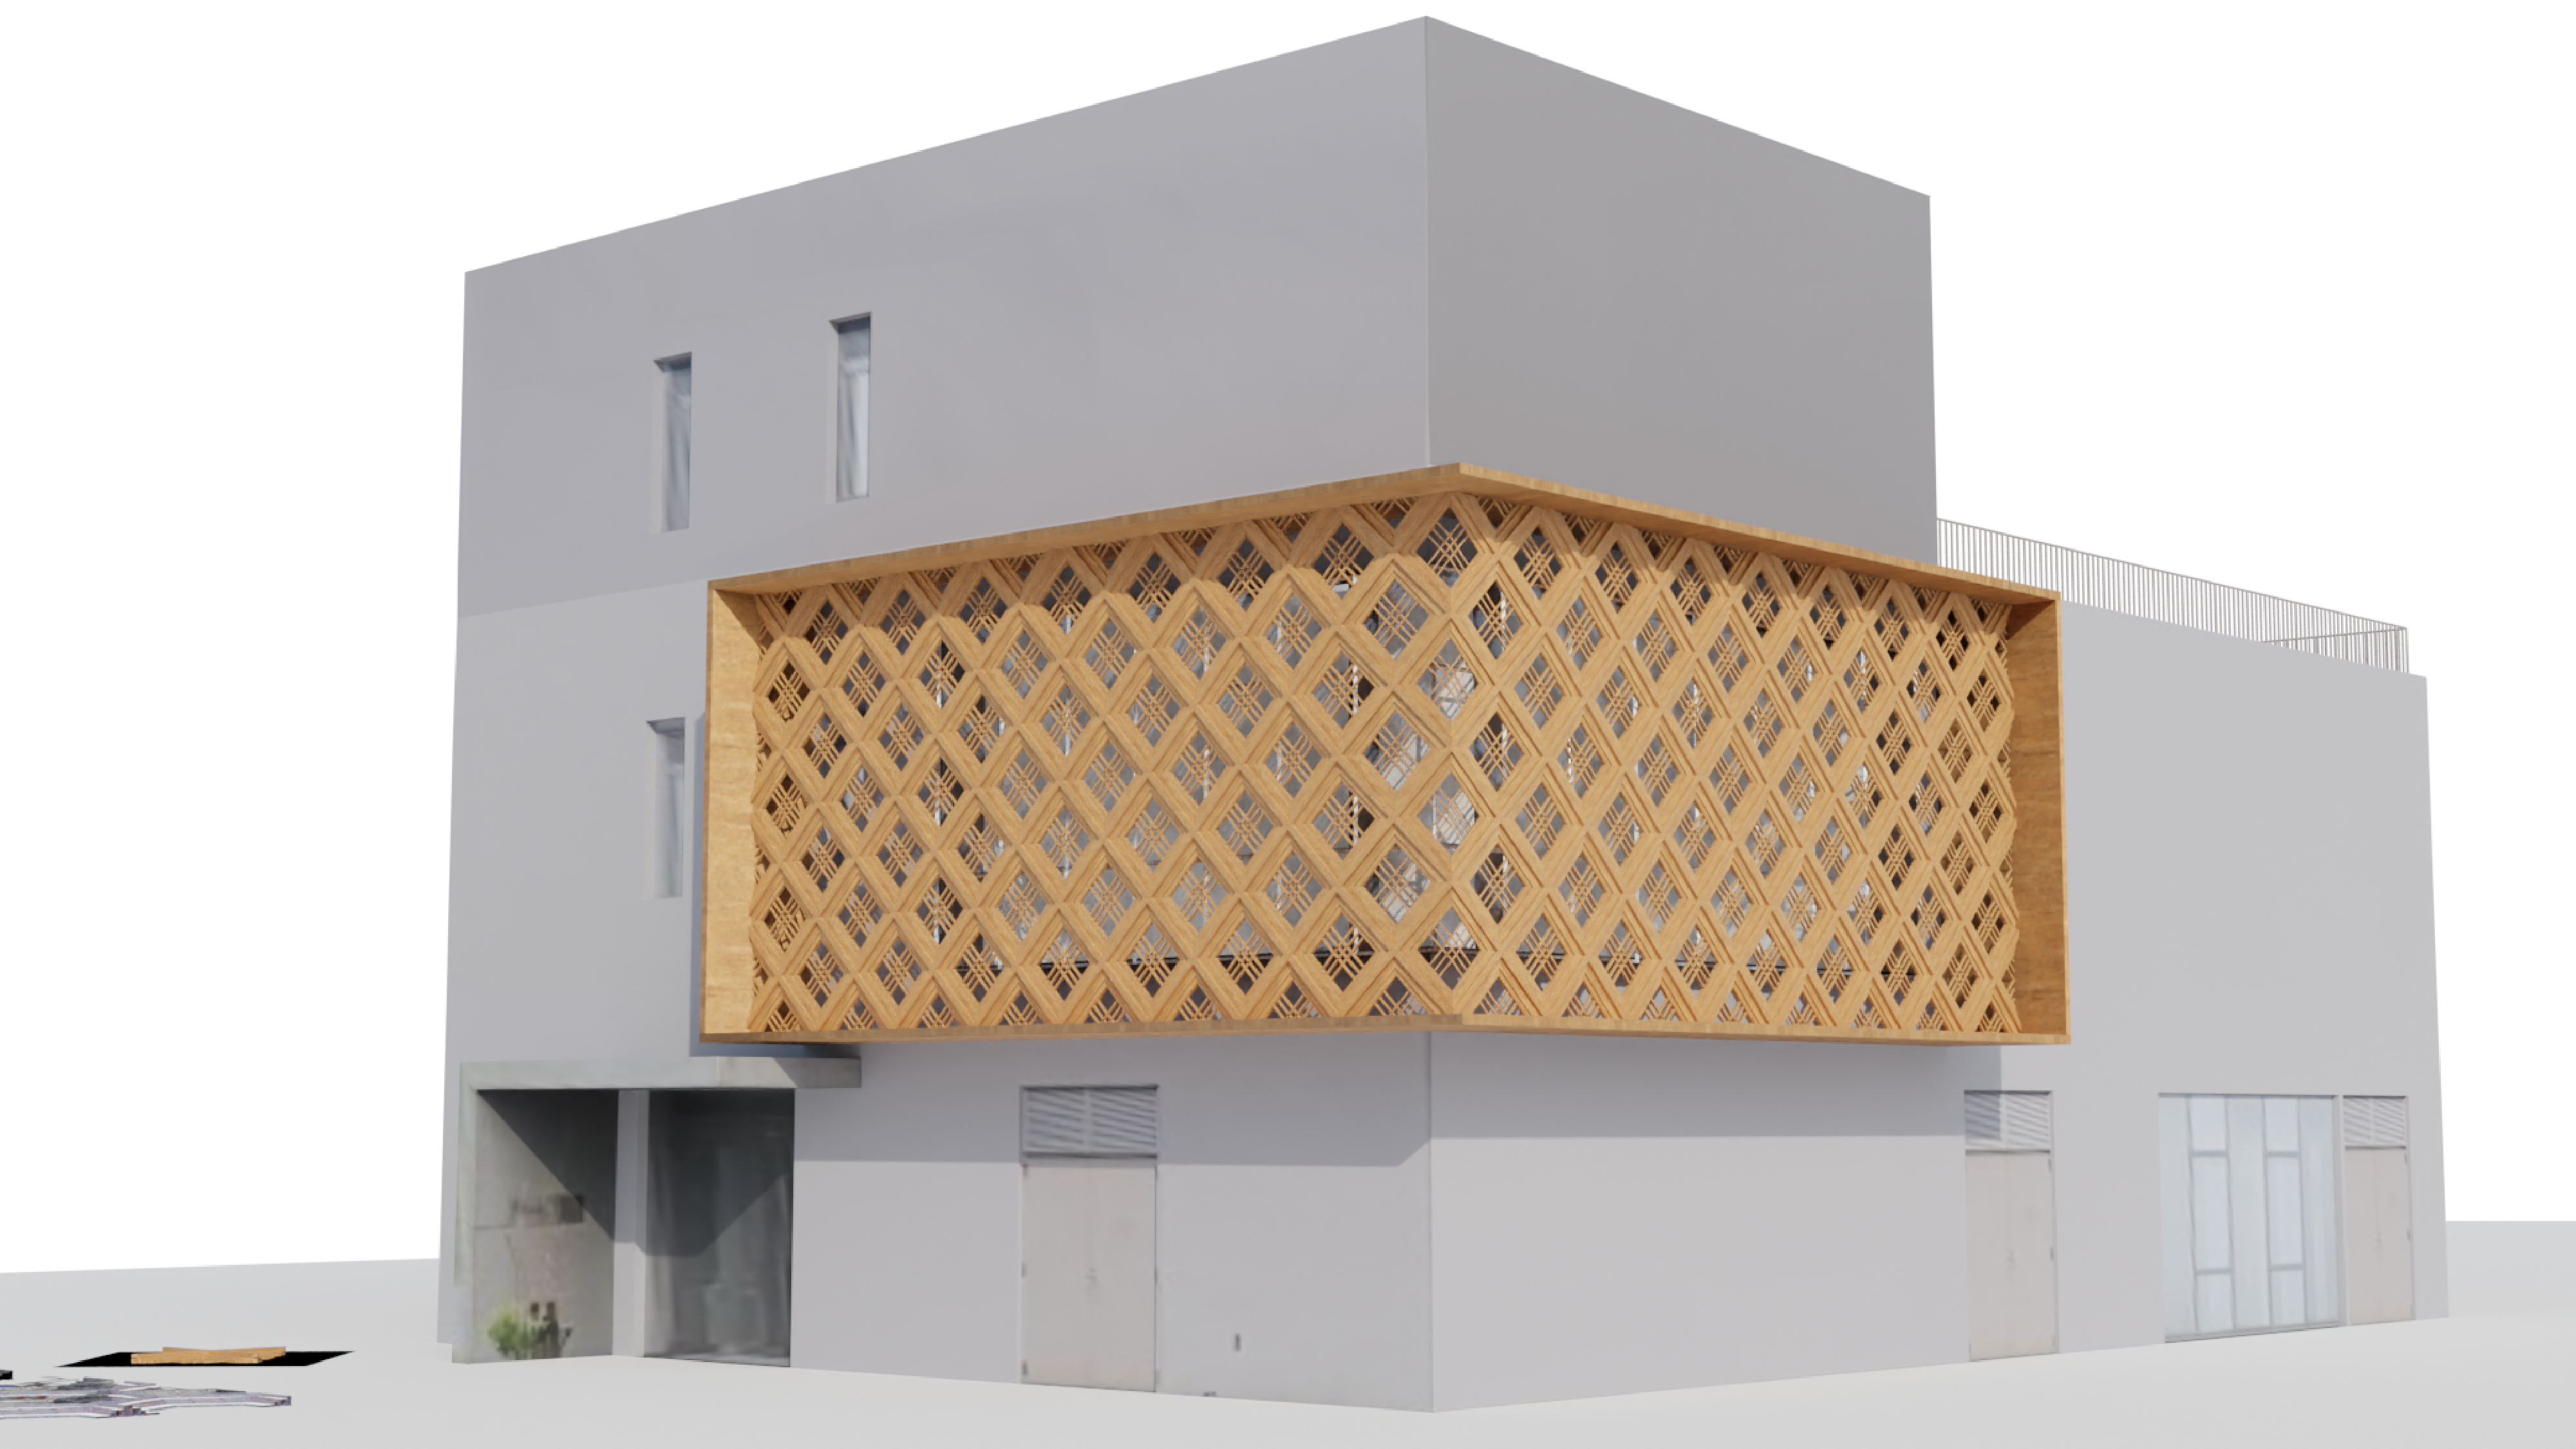
\includegraphics[width=1\linewidth]{Images/Pattern 1/0003}} &
              {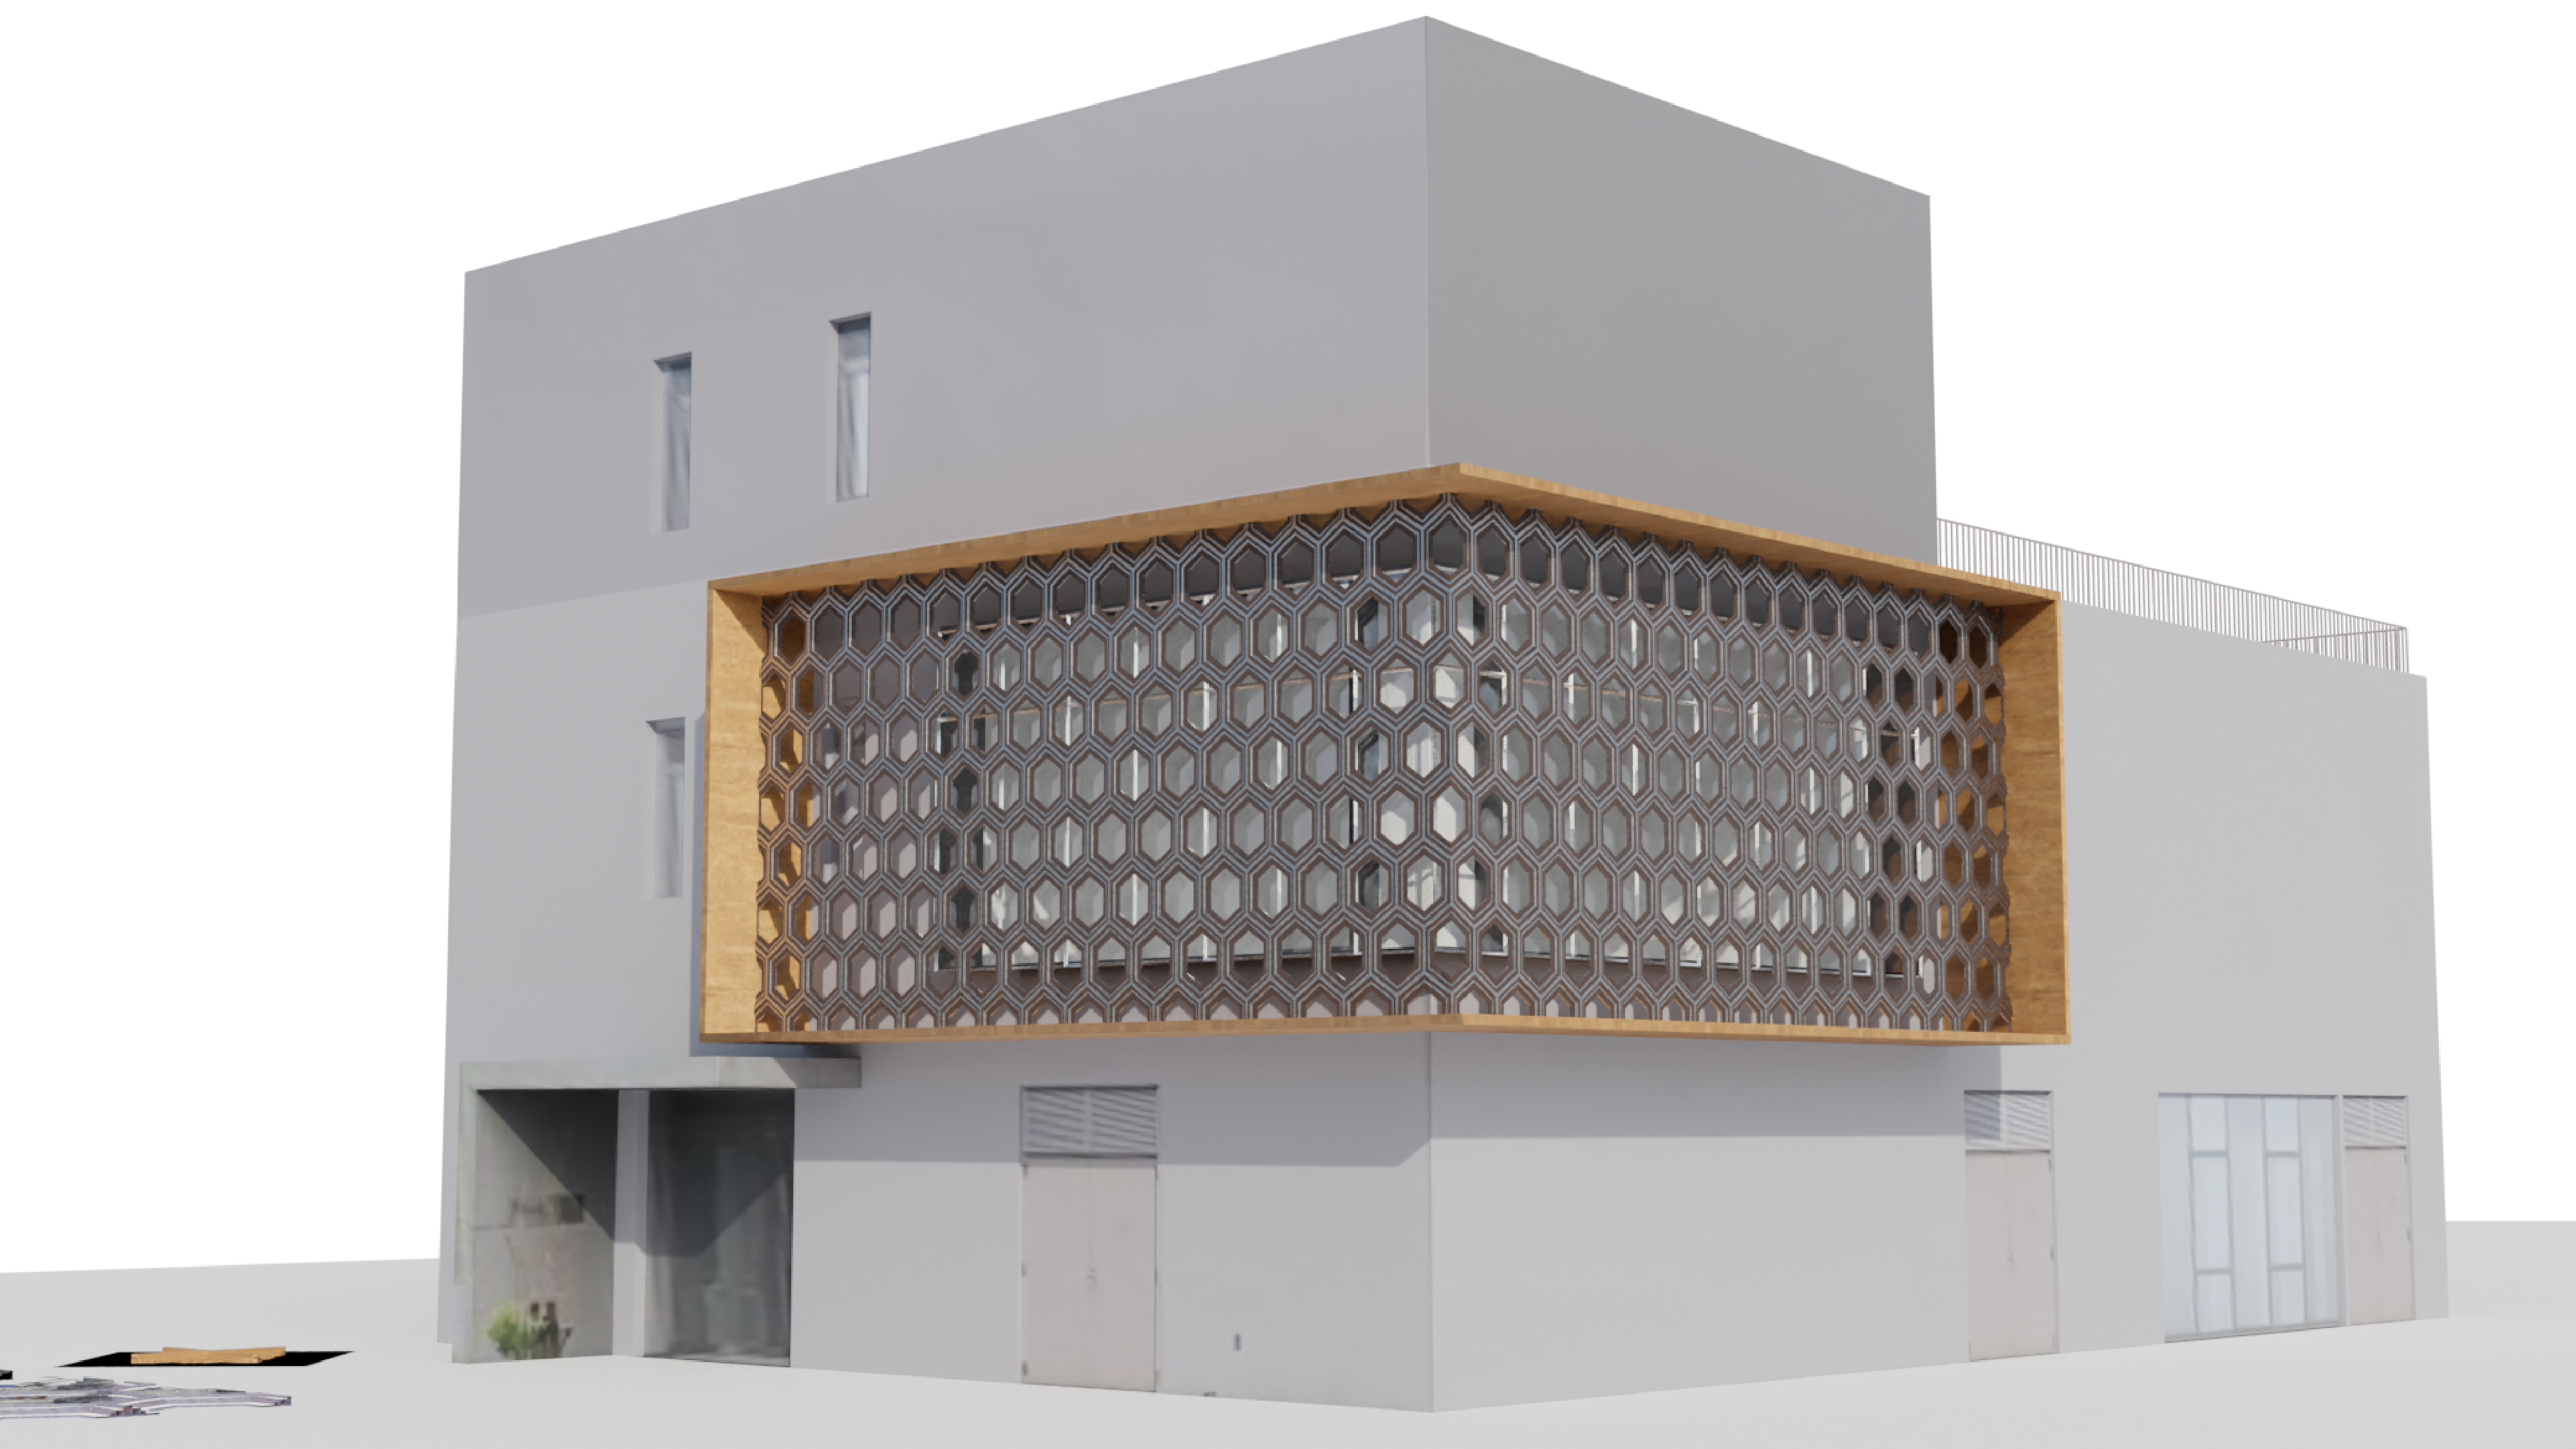
\includegraphics[width=1\linewidth]{Images/Pattern 2/0003}} &
              {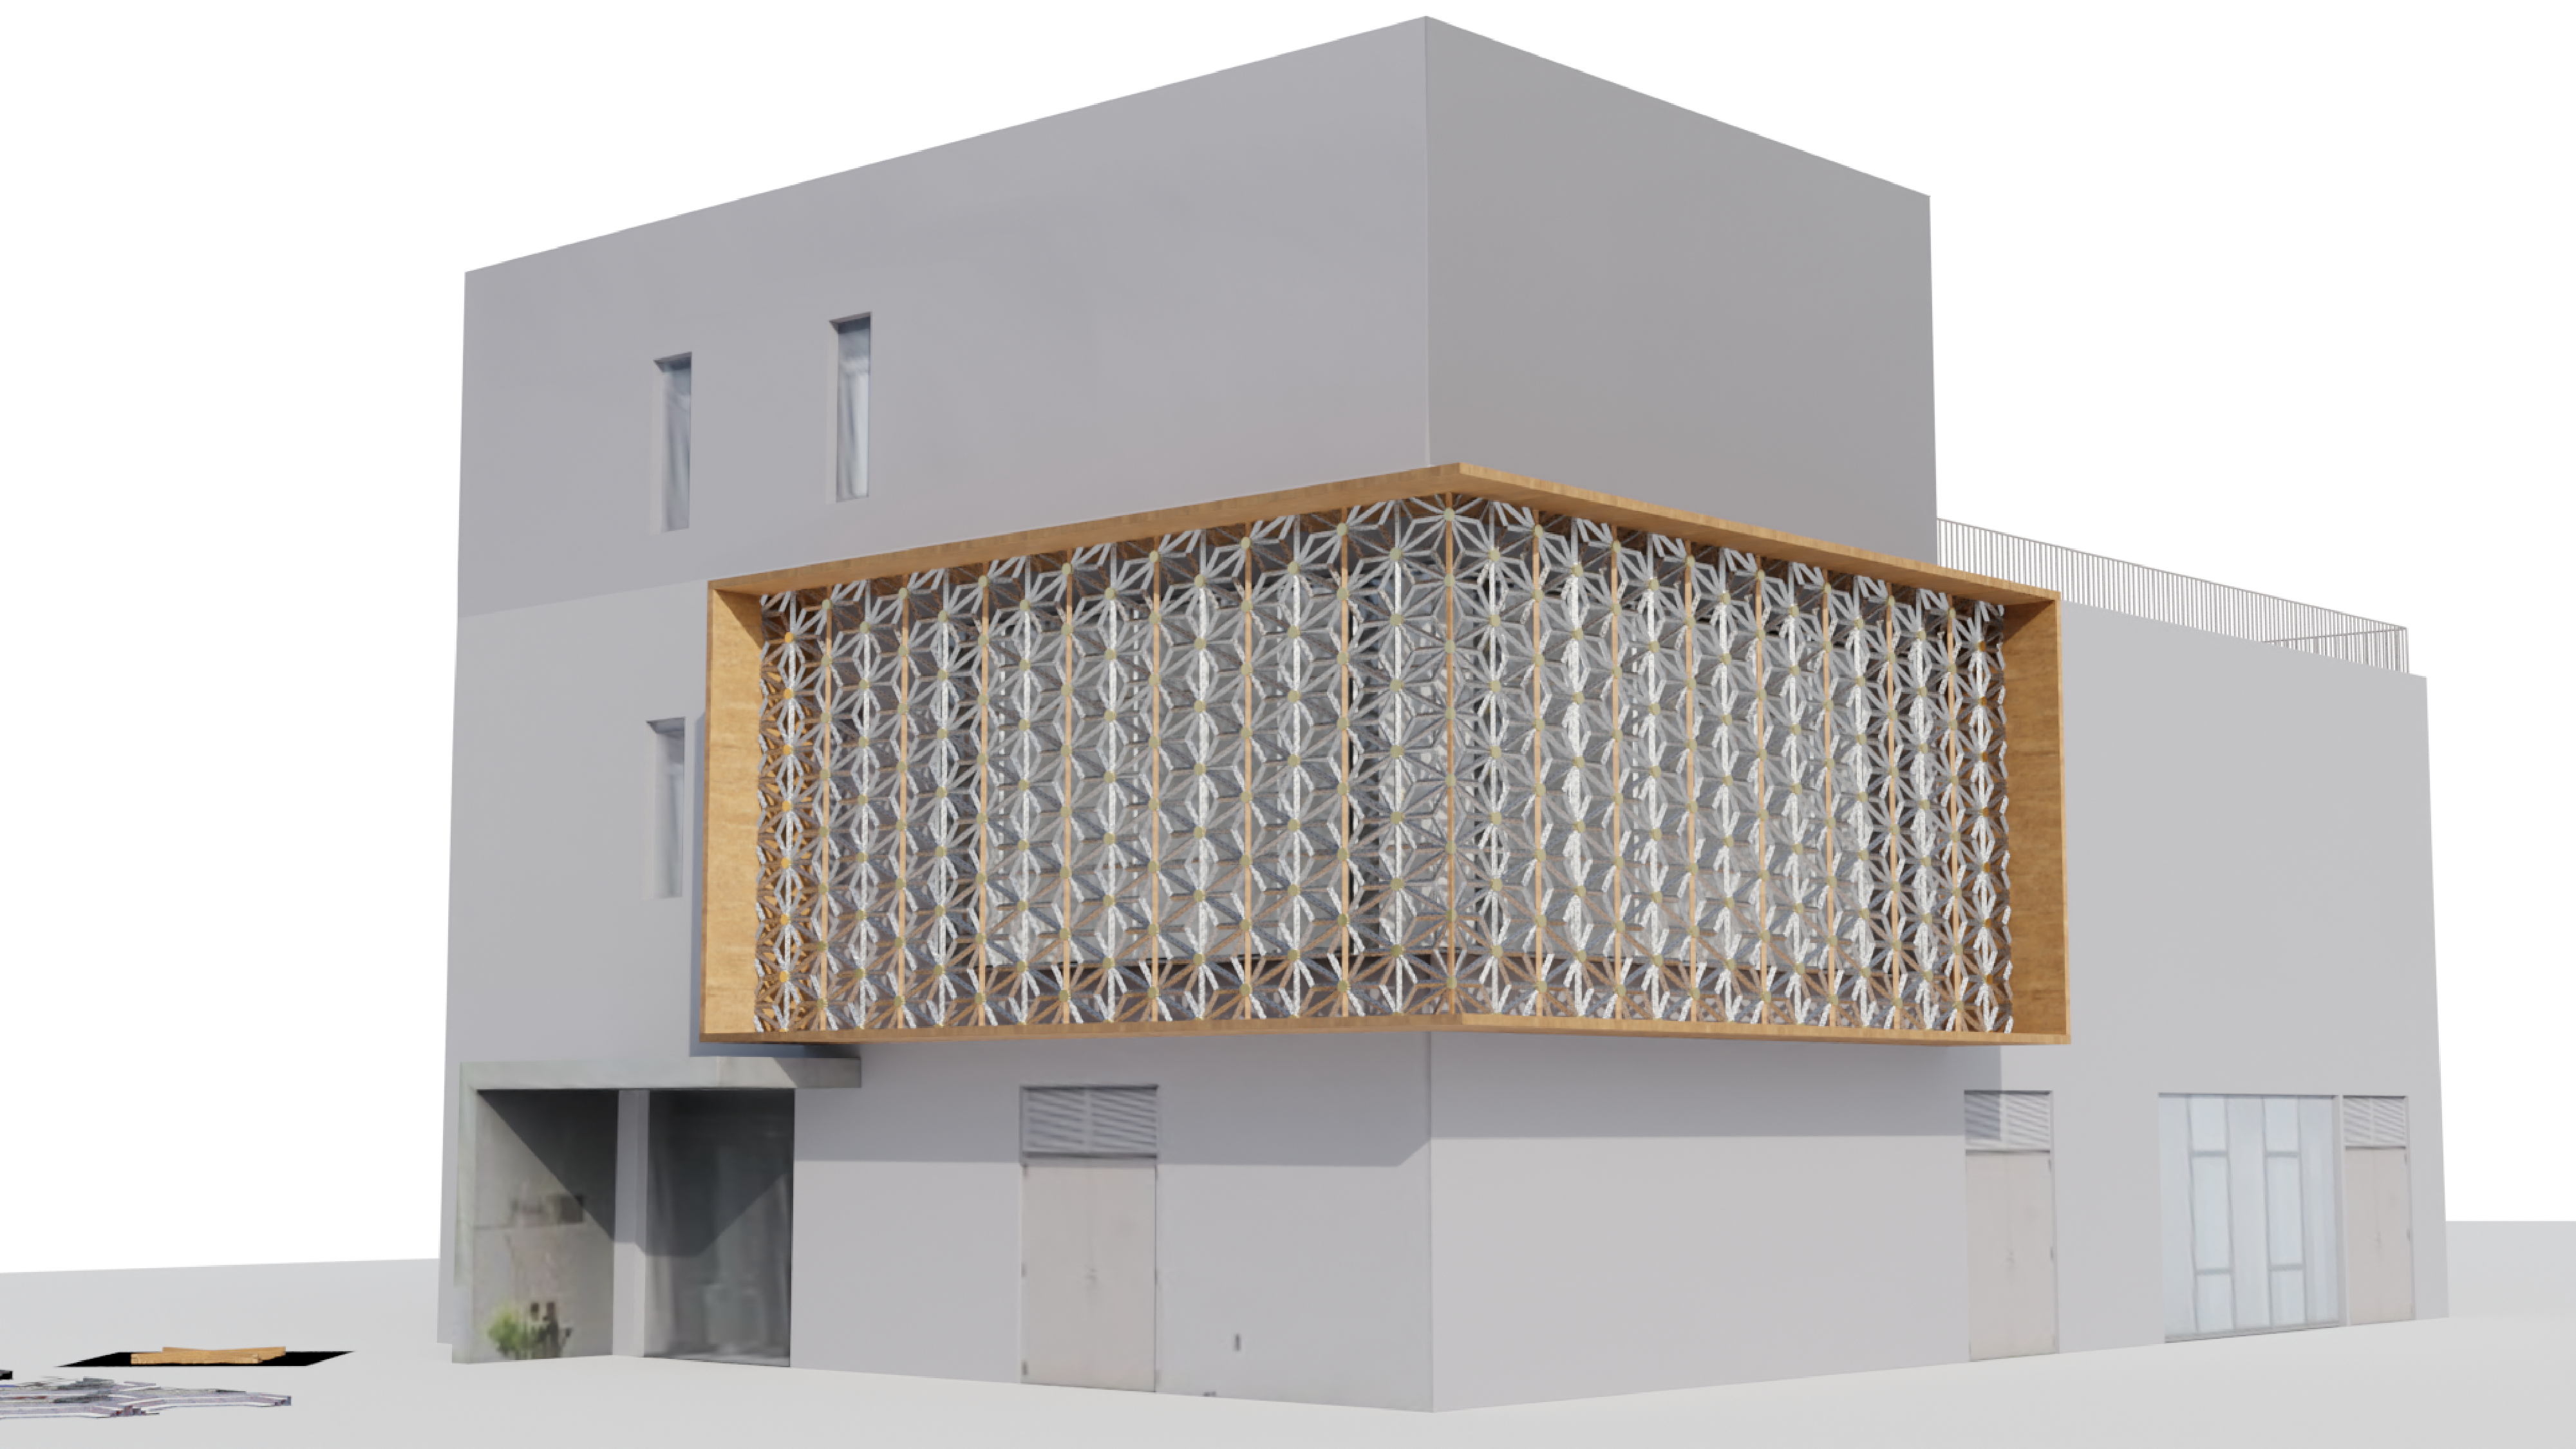
\includegraphics[width=1\linewidth]{Images/Pattern 3/0003}} \\
            \midrule
            \text{Level 6} &  &  &
            \\
            {\includegraphics[width=1\linewidth]{Images/Wall 0/0006}} &
              {\includegraphics[width=1\linewidth]{Images/Pattern 1/0006}} &
              {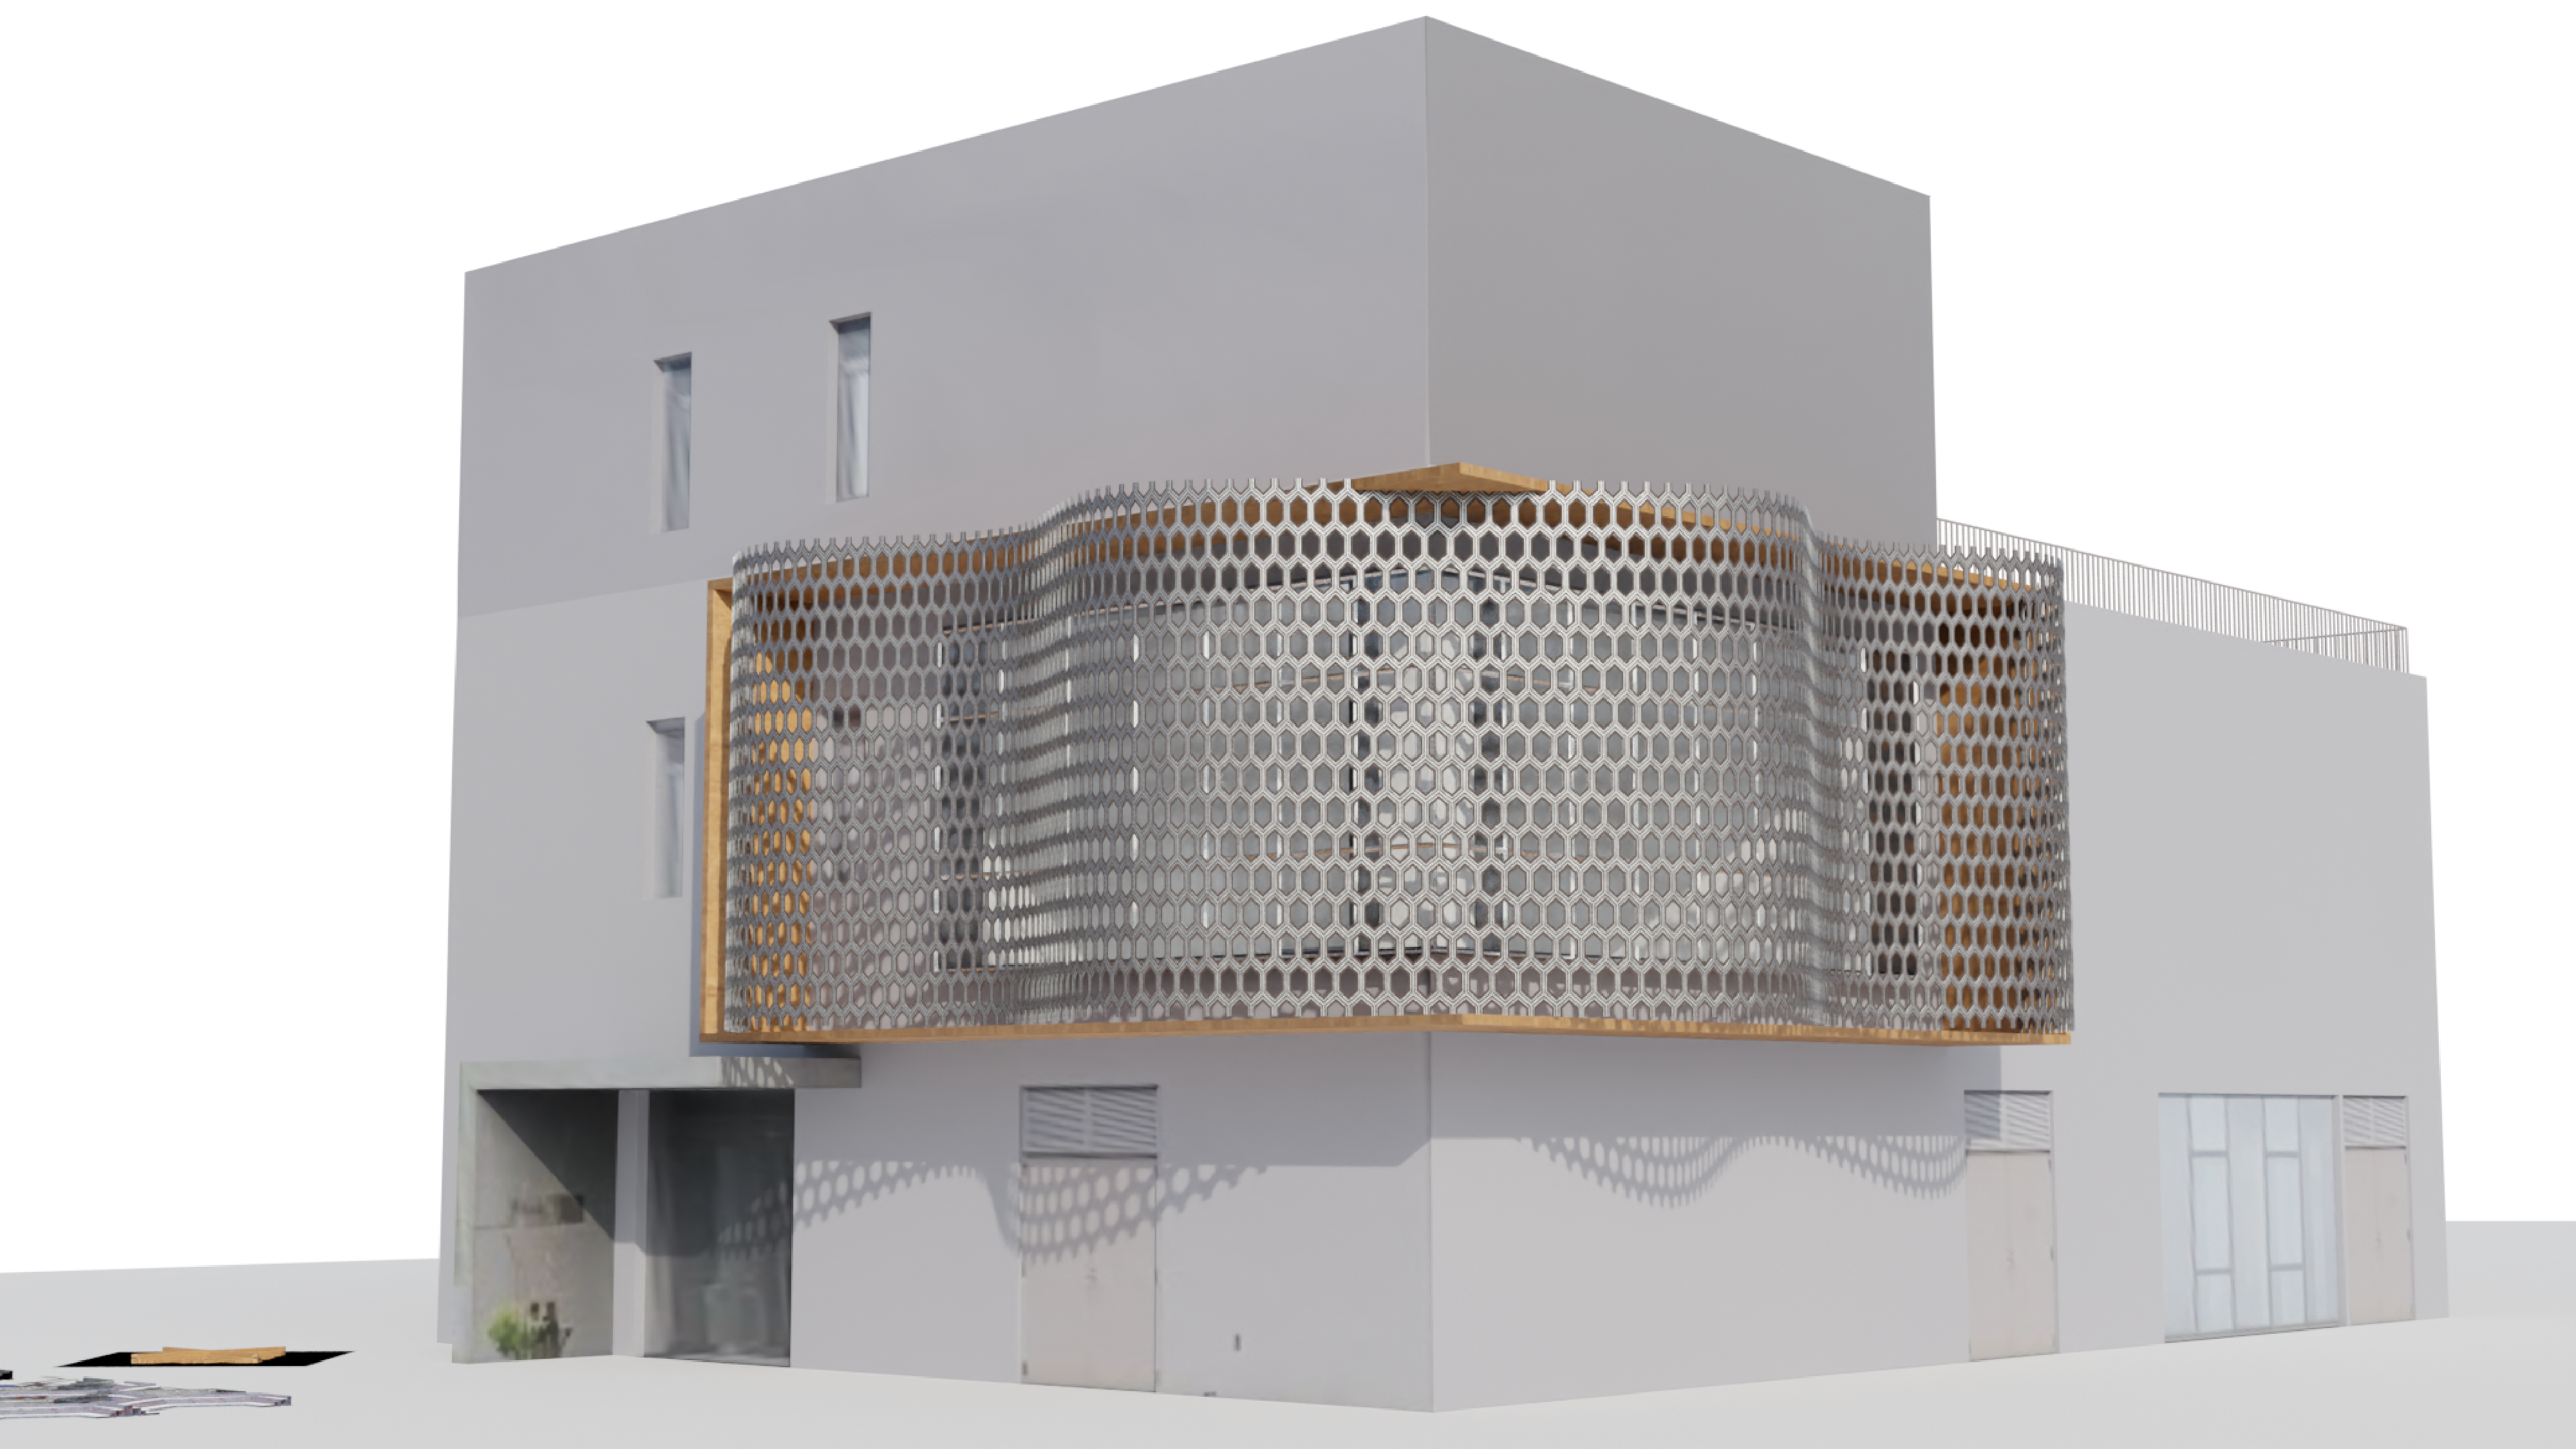
\includegraphics[width=1\linewidth]{Images/Pattern 2/0006}} &
              {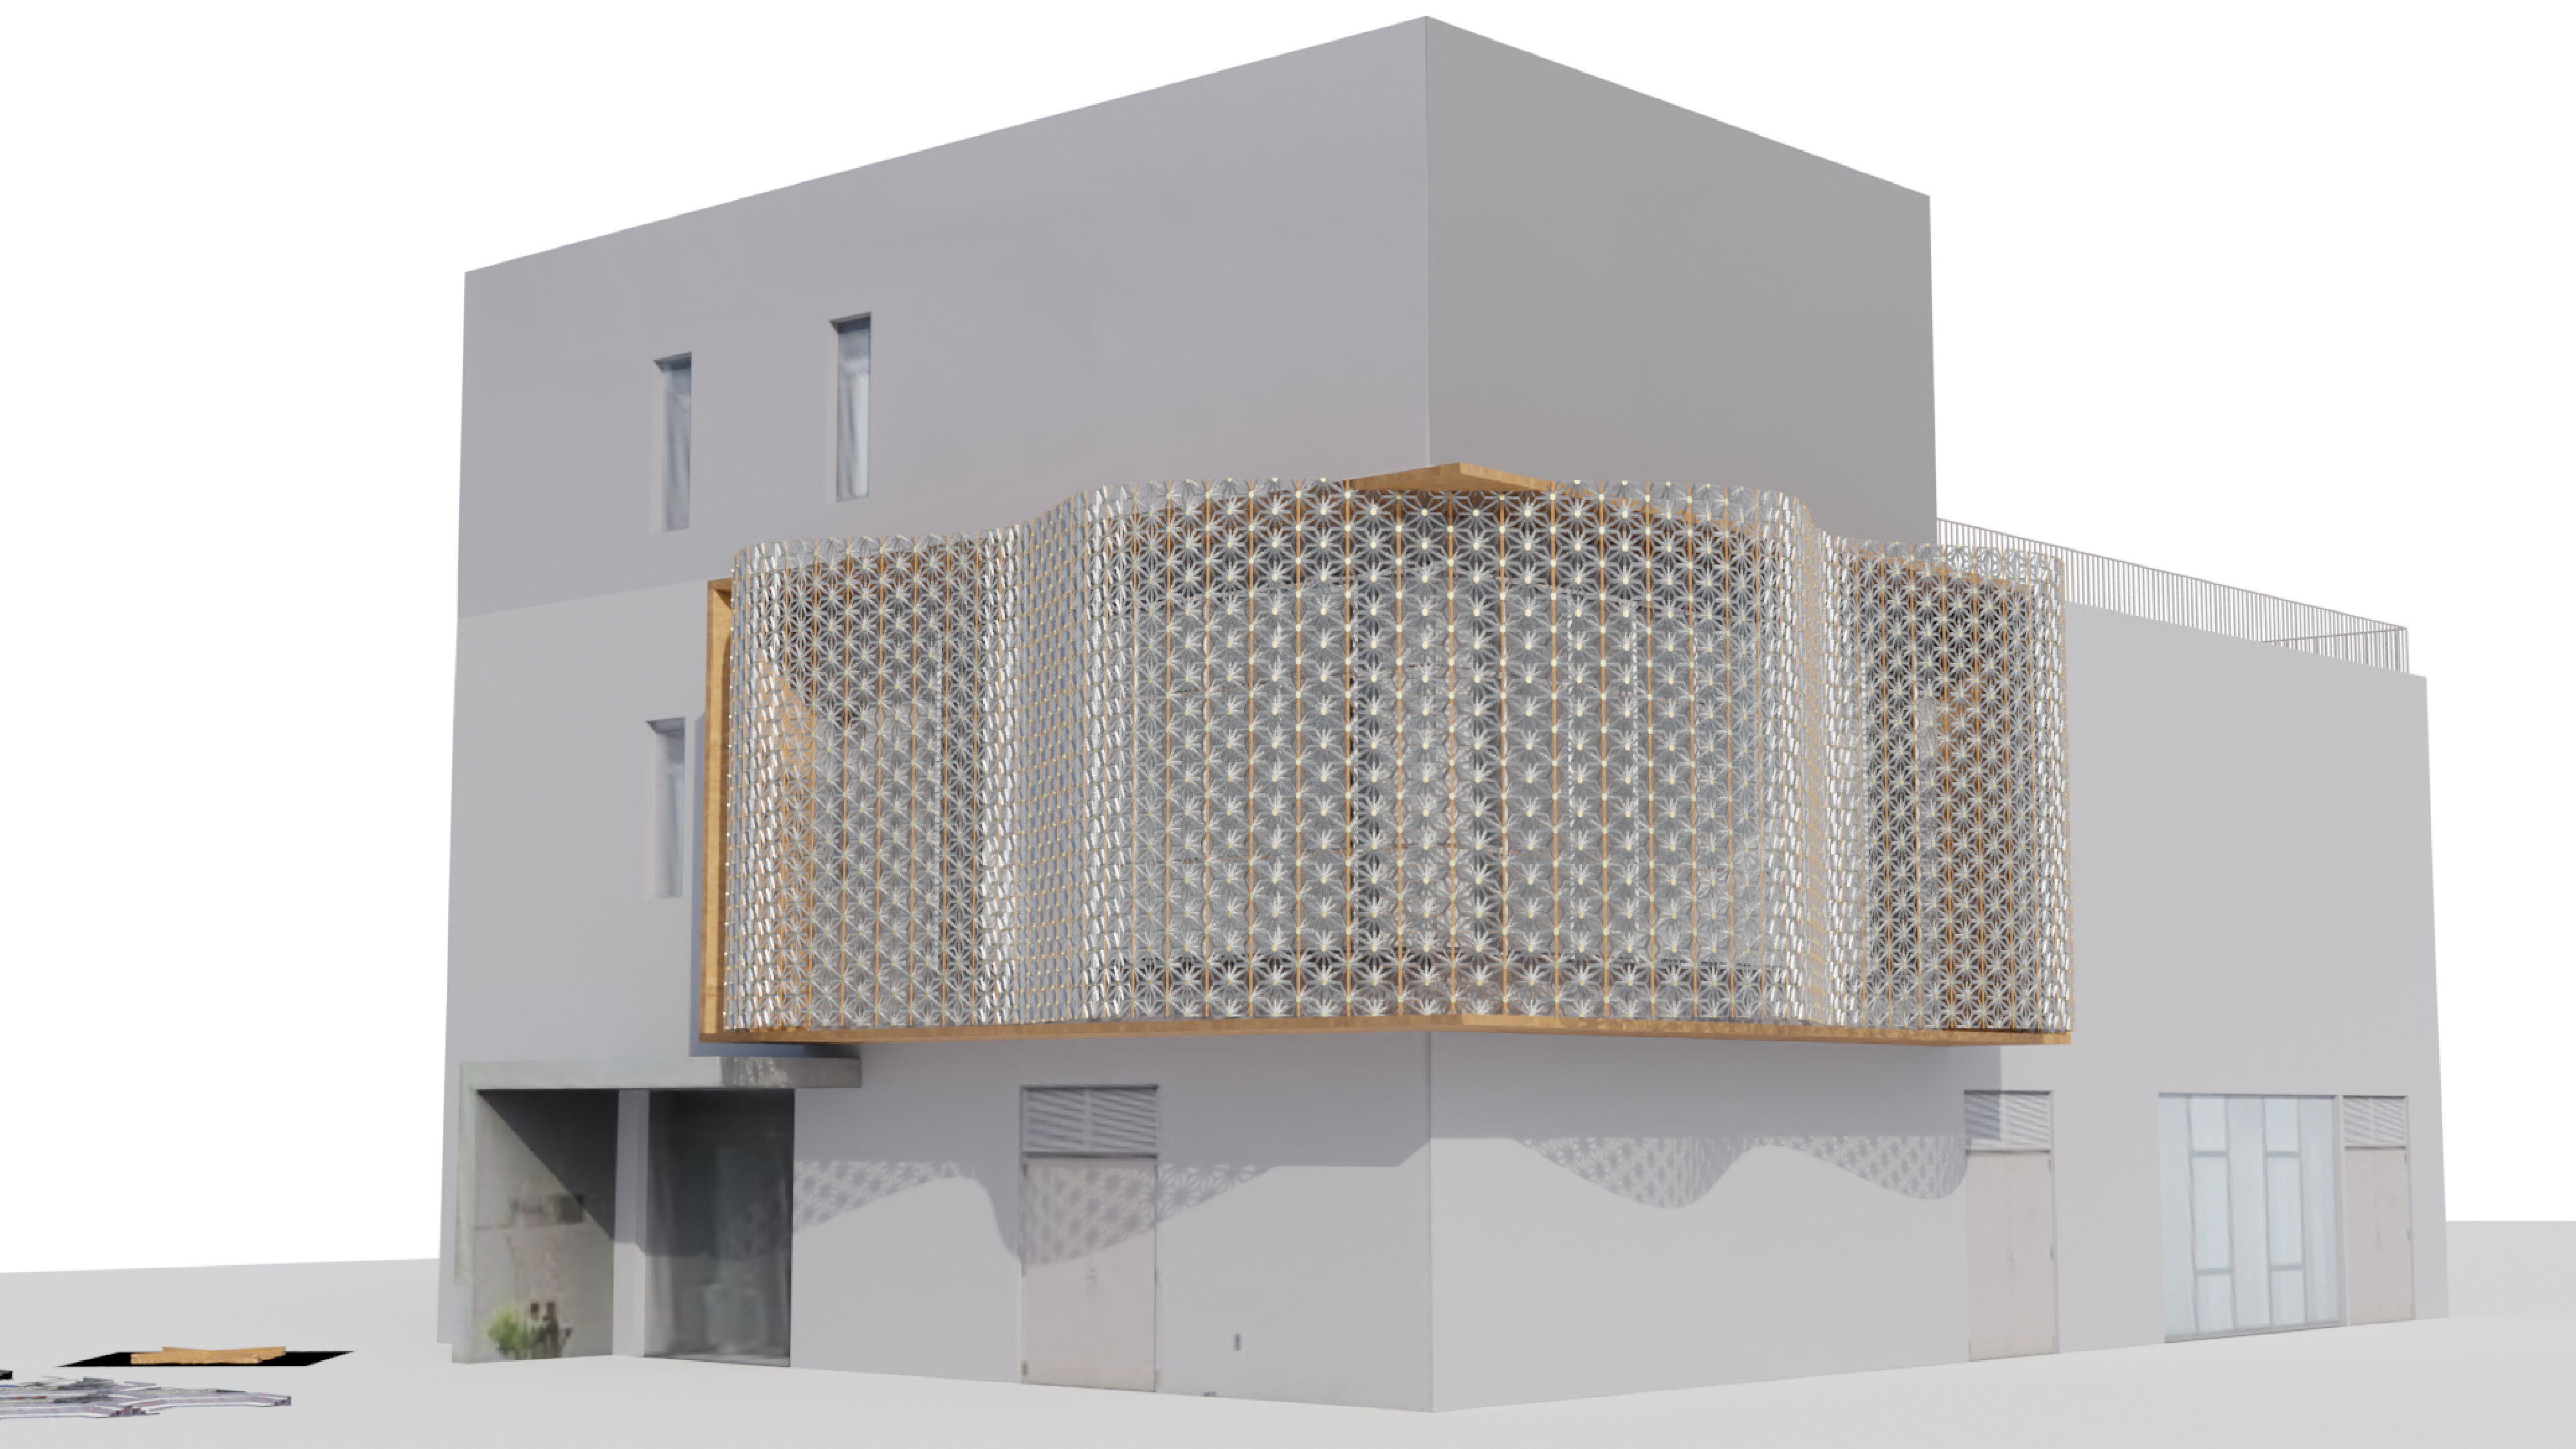
\includegraphics[width=1\linewidth]{Images/Pattern 3/0006}} \\
            \midrule
            \text{Level 9} &  &  &
            \\
            {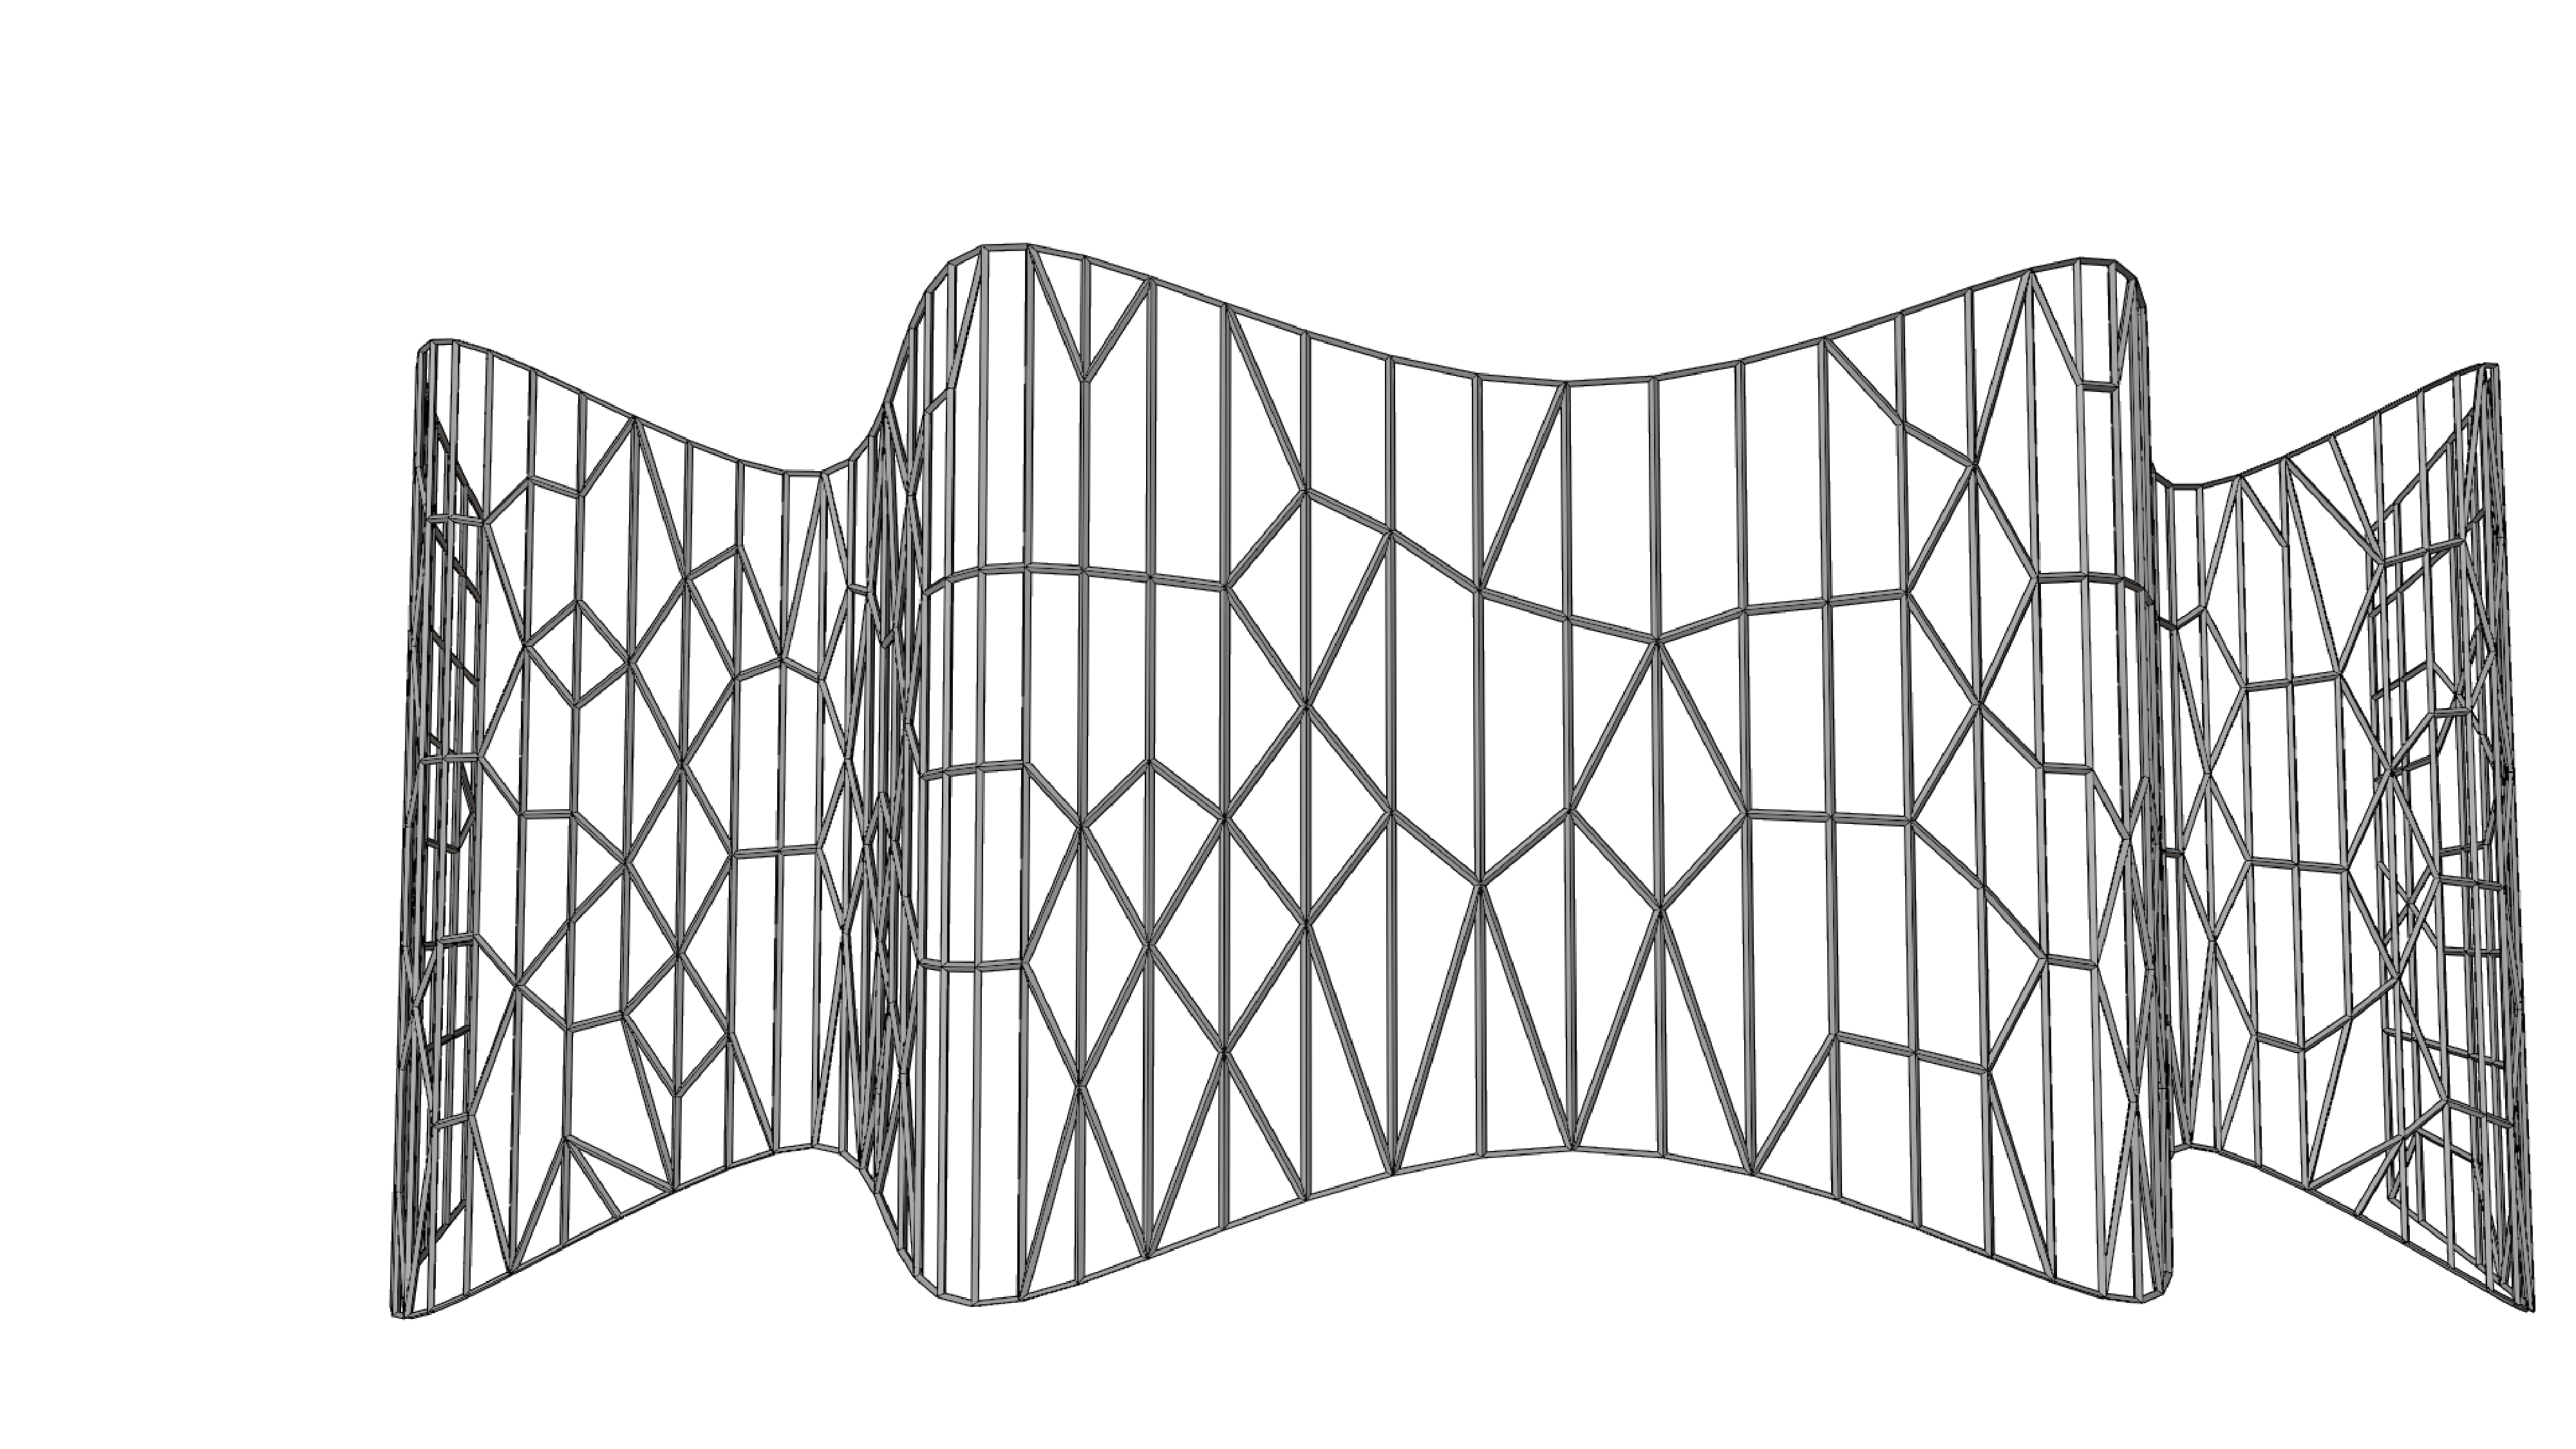
\includegraphics[width=1\linewidth]{Images/Wall 0/0009}} &
              {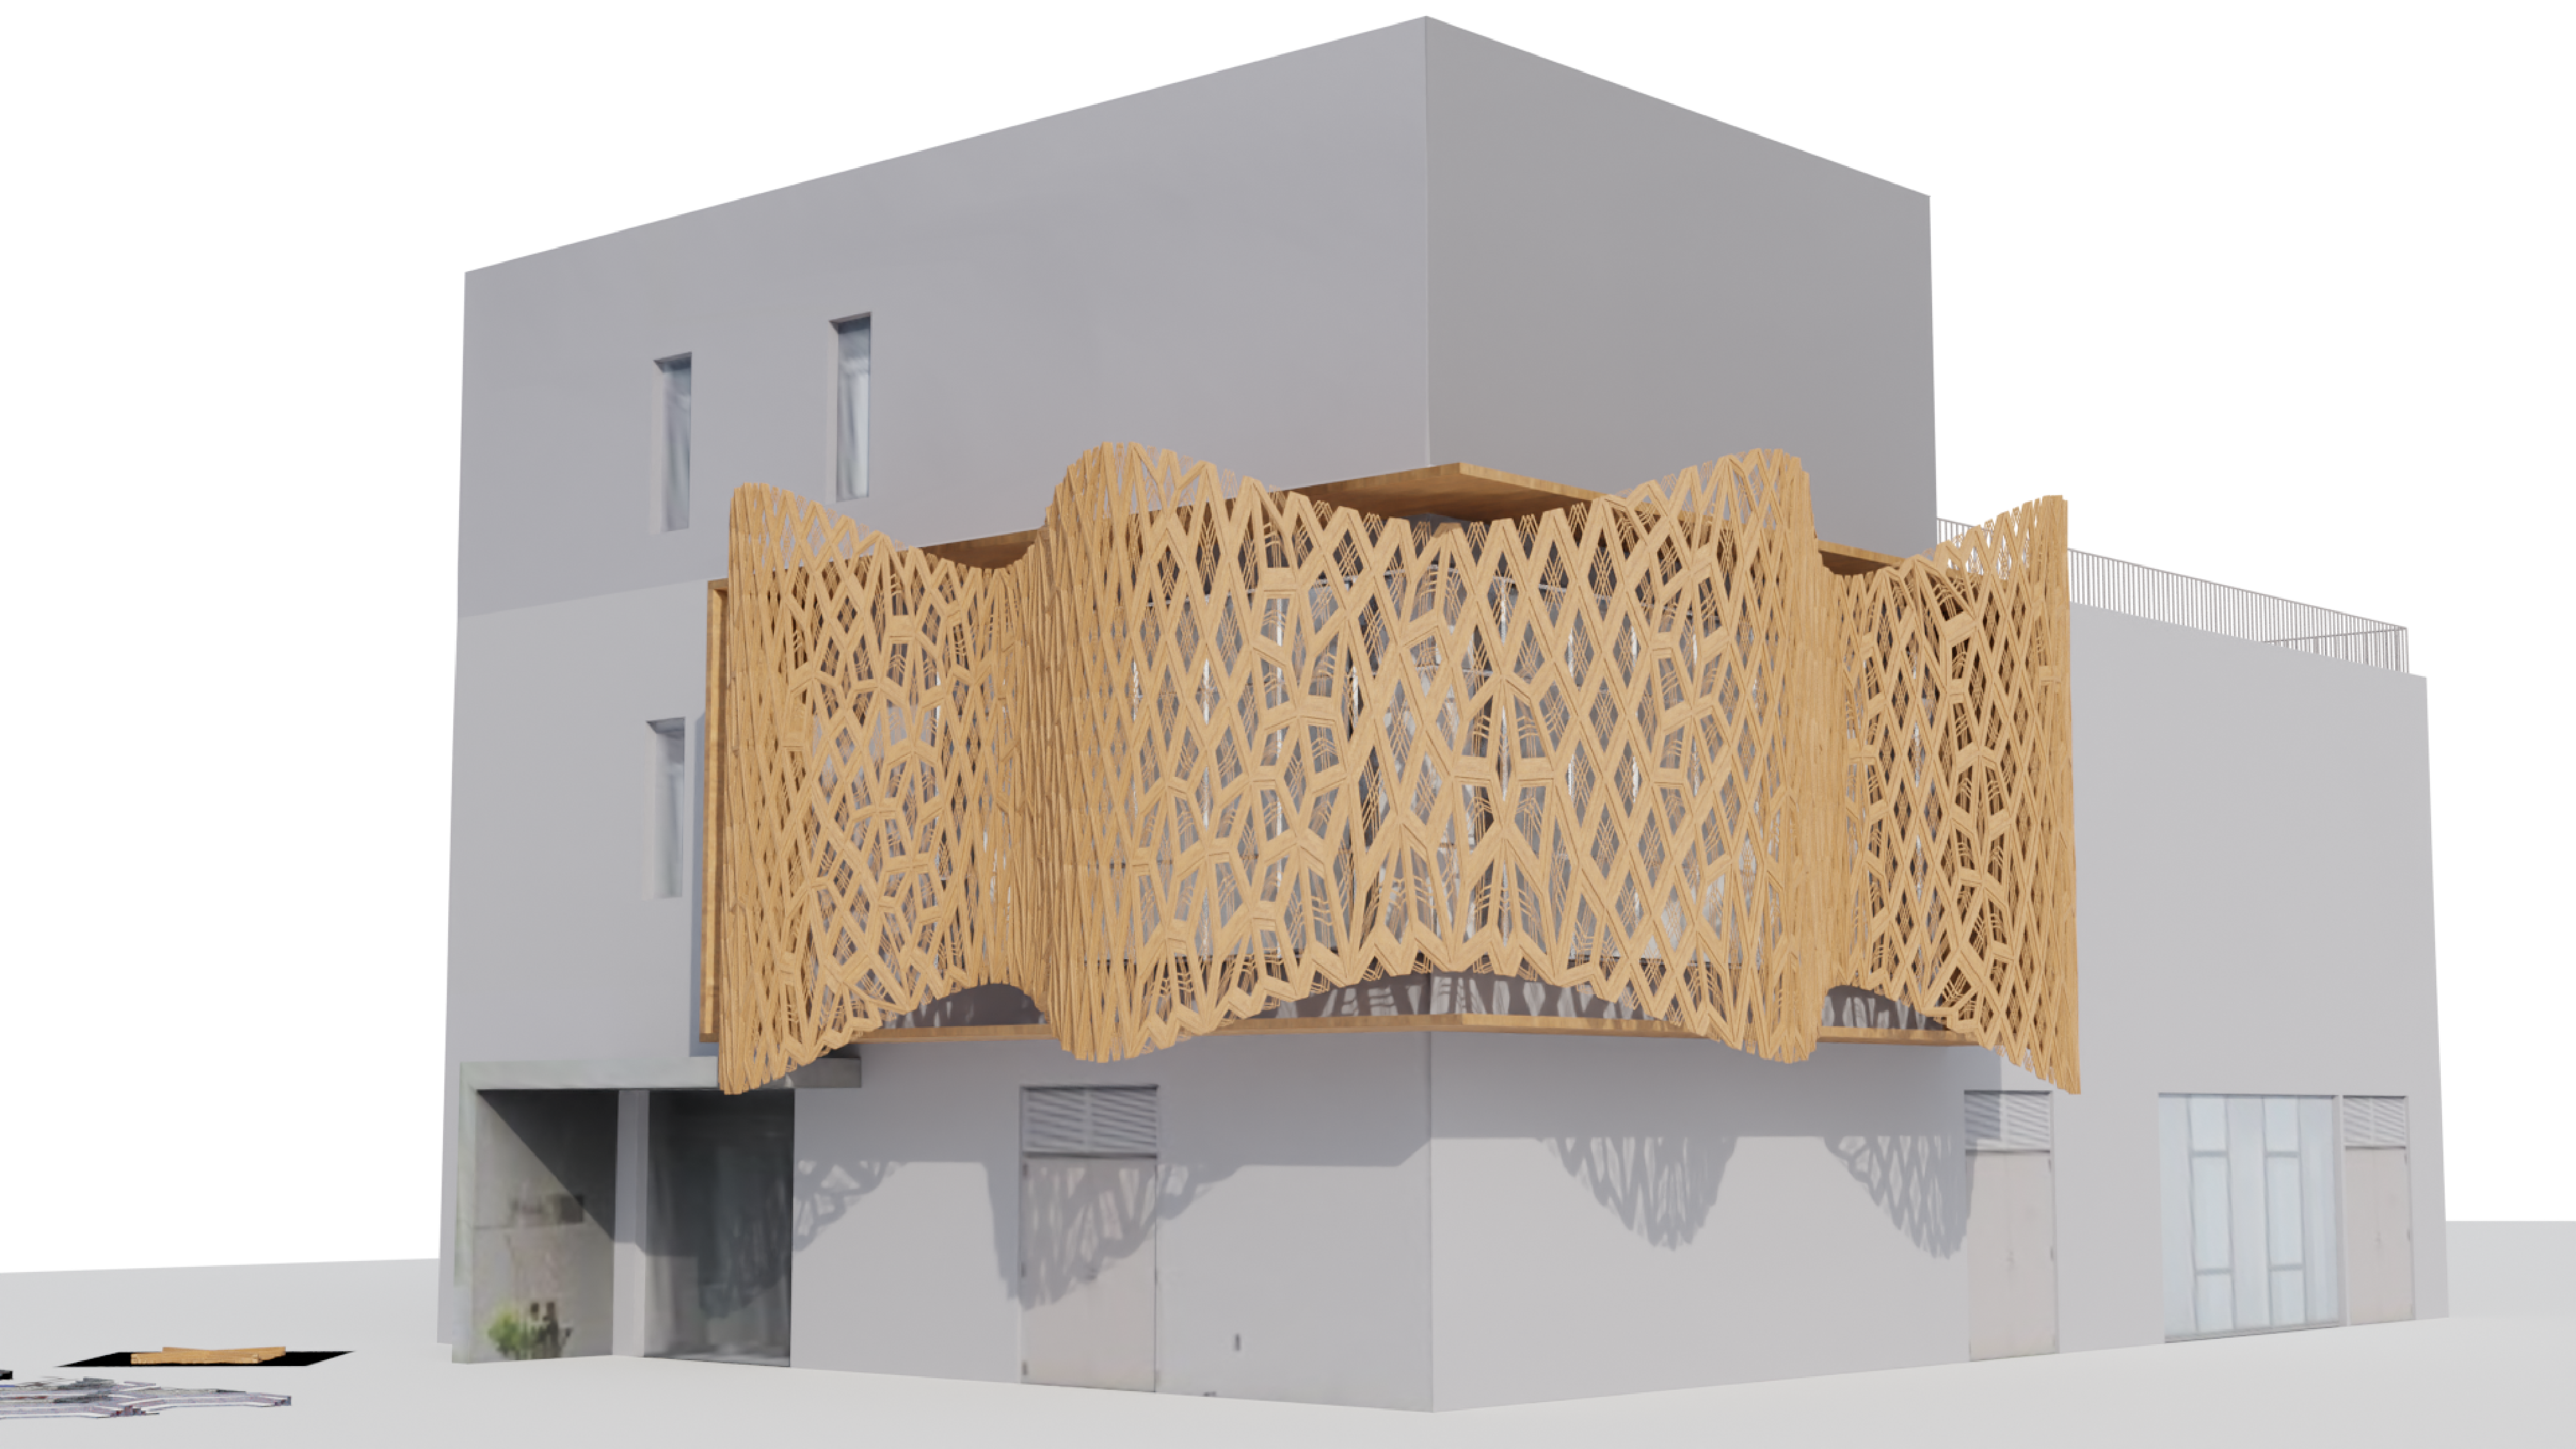
\includegraphics[width=1\linewidth]{Images/Pattern 1/0009}} &
              {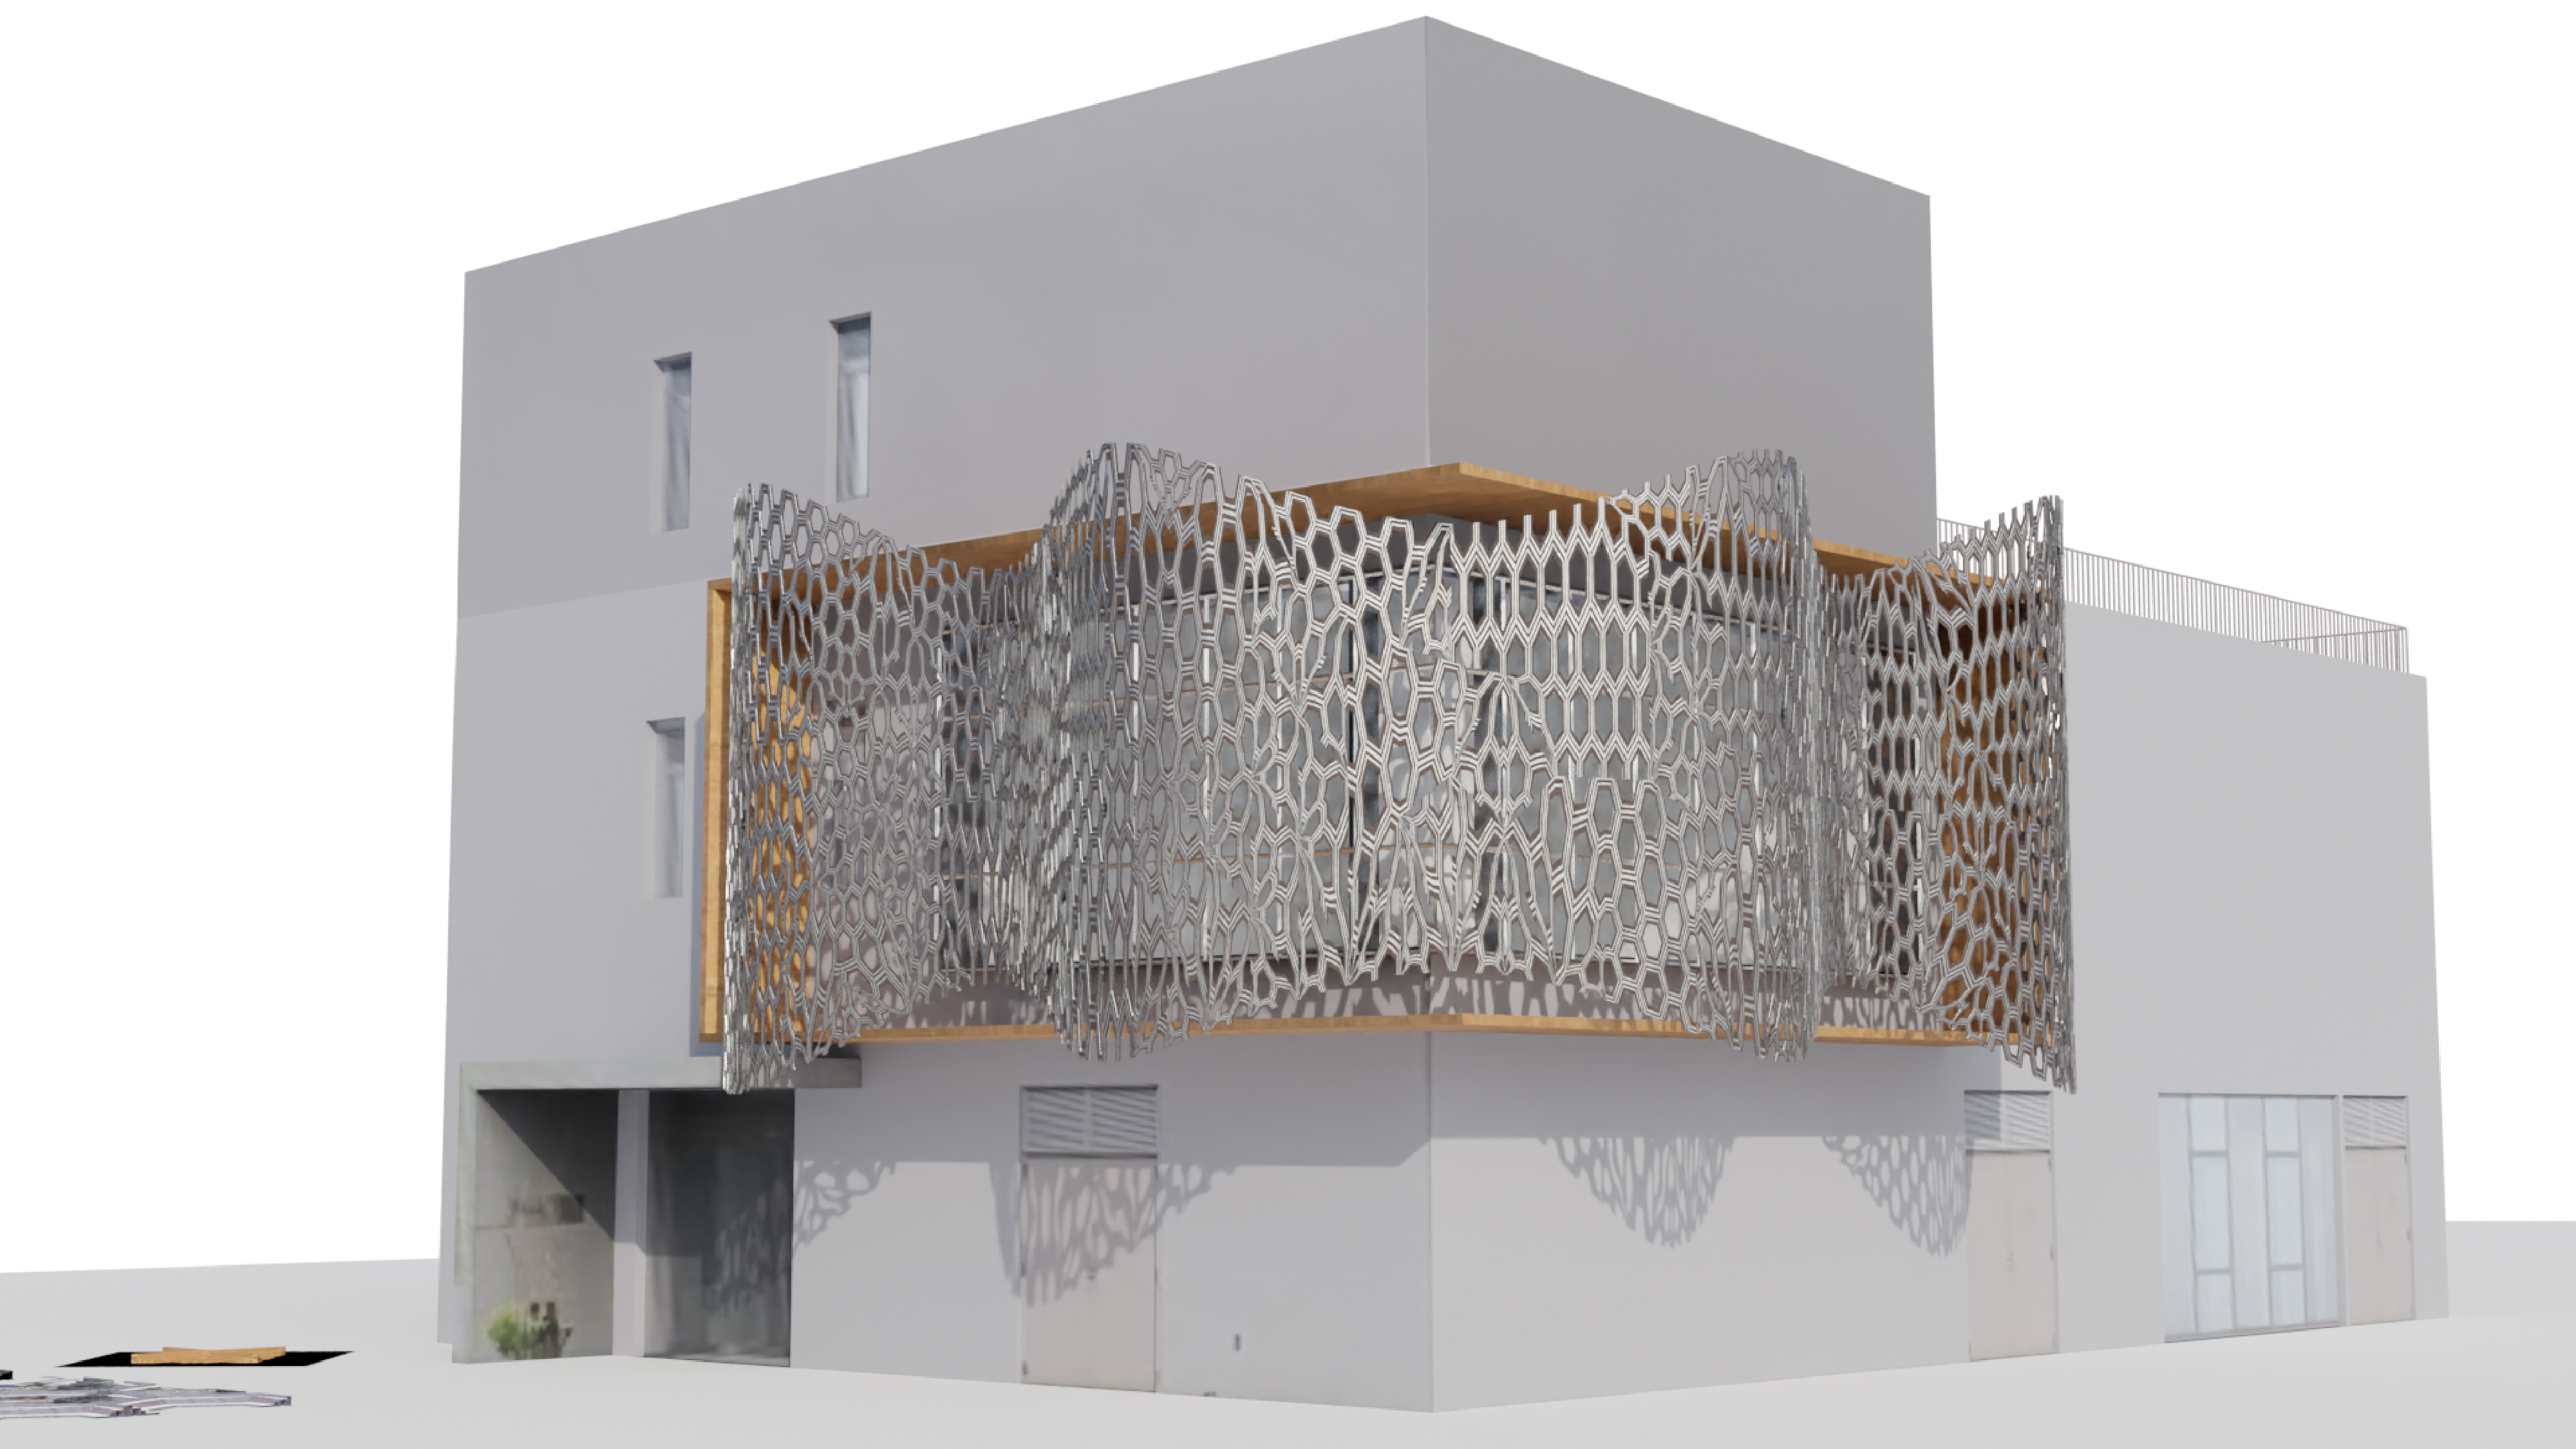
\includegraphics[width=1\linewidth]{Images/Pattern 2/0009}} &
              {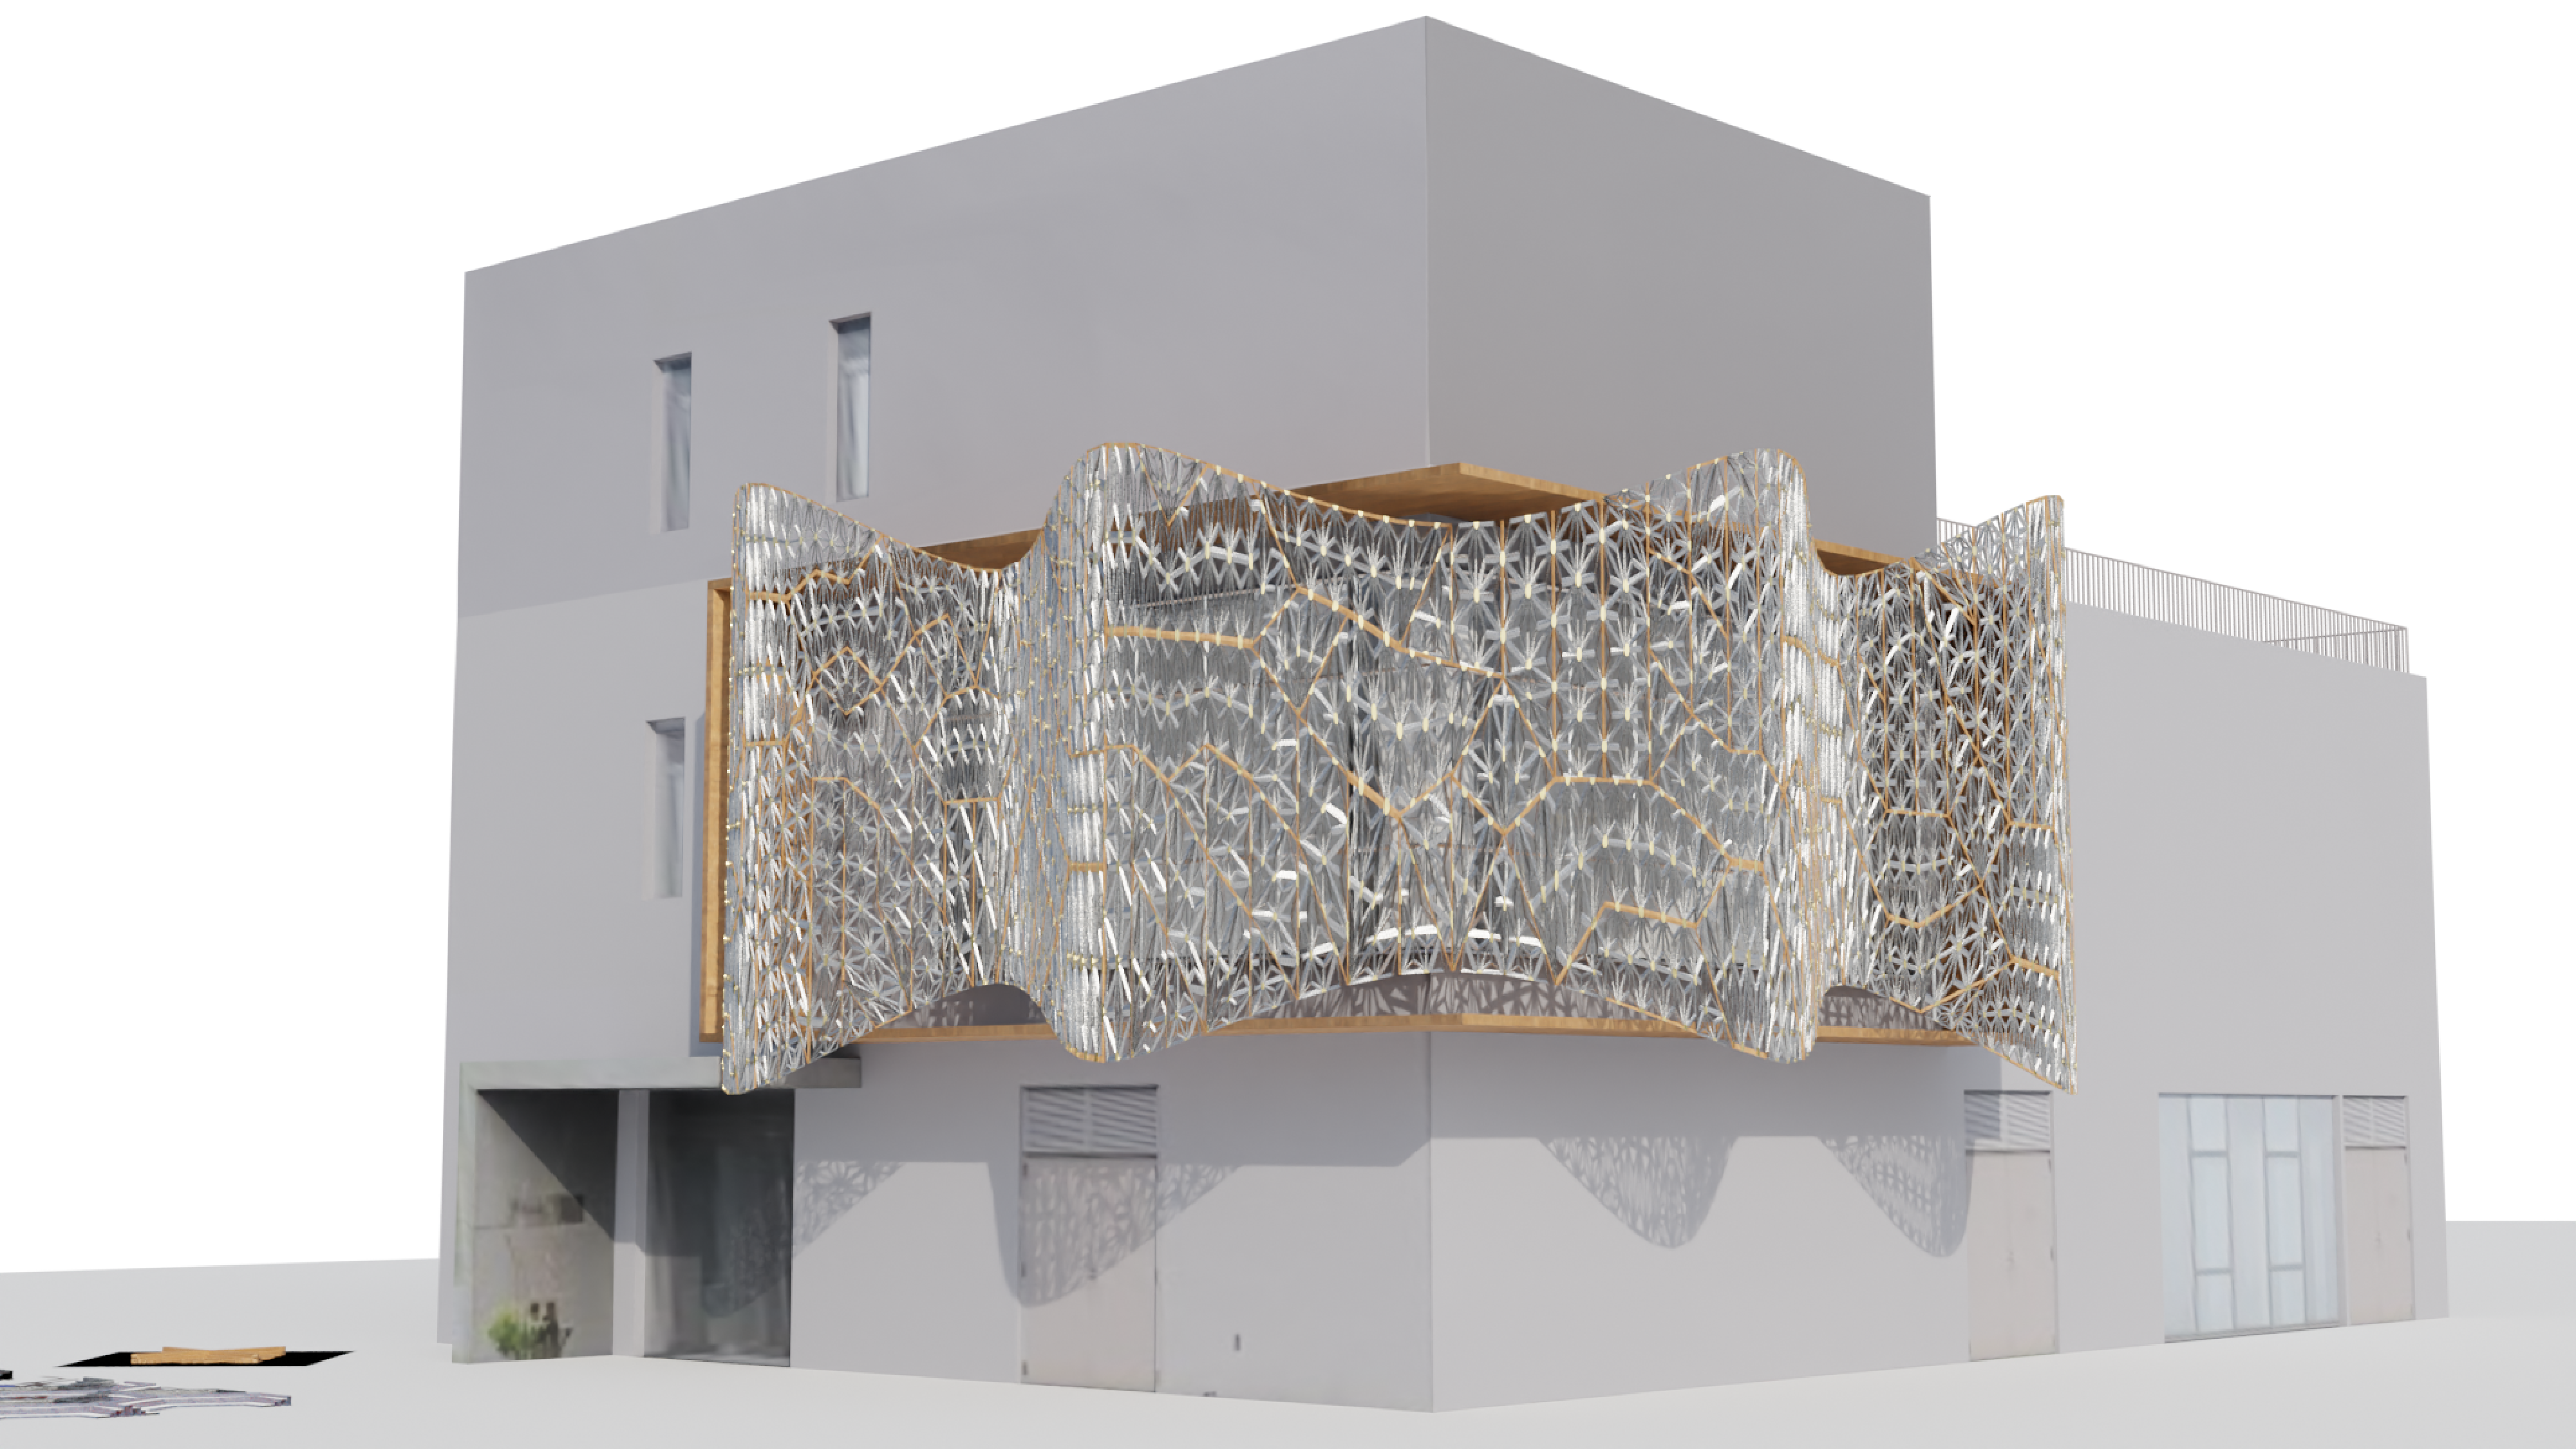
\includegraphics[width=1\linewidth]{Images/Pattern 3/0009}} \\
            \bottomrule
        \end{tabularx}
    \end{table*}


Ensuring a high level of realism is paramount in Virtual Reality simulation, particularly when aiming to replicate a genuine experience.
In the context of this research, our objective is to assess the reactions of individuals within a building adorned with facades of varying complexity.
Therefore, the precision of our 3D modeling is of utmost significance.

For this purpose, the ``3D modeling'' module realized in Blender (v3.6), serves as the first component and is responsible for generating the 3D models central to our research that include the site and building as a virtual environment where the experiment will be conducted and generating the distinctive facade variations.

The virtual environment created is an exact replica of the Architectural Environment Research Building, also known as Building HE20, which houses our laboratory on the Itoshima campus of Kyushu University (see Figure\ref{fig:RealVs3dModel}).

    %% Figure of Real building next to 3D modeled building
     \begin{figure}[t]
          \centering
          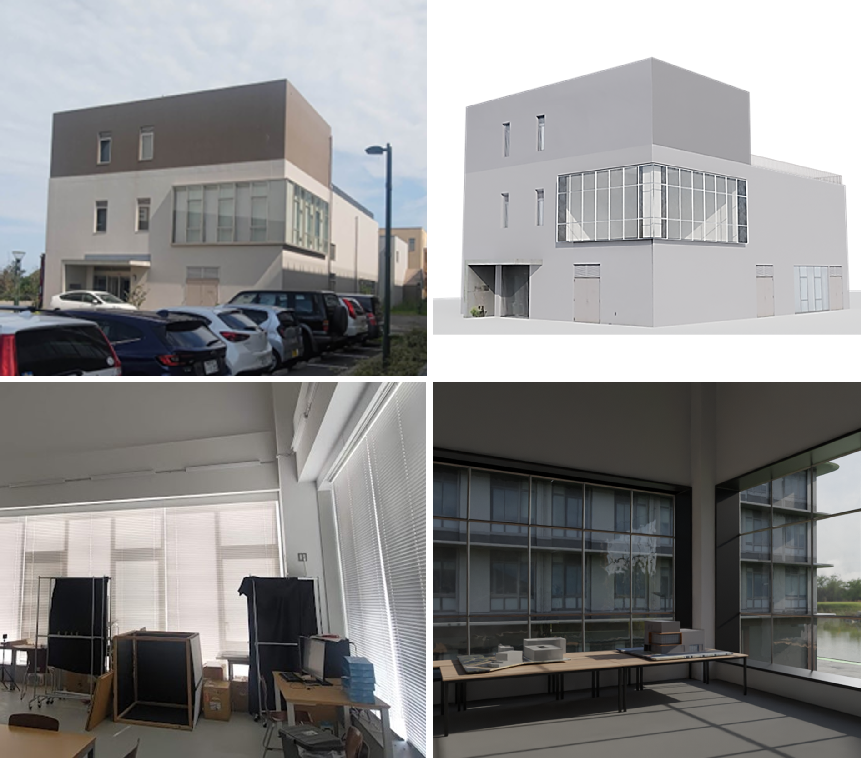
\includegraphics[width= \linewidth]{Images/Realvs3DmodelBlender}
          \caption{Side-by-side comparison of the Architectural Environment Building at Kyushu University used in the experiment, featuring actual interior and exterior photographs (left), and its virtual clone meticulously modeled and rendered in Blender (v3.6) for the Facade Design Complexity Analysis experiment.}
          \label{fig:RealVs3dModel}
        \end{figure}

To ensure an authentic experience, both the exterior of the building and the interior laboratory spaces were meticulously modeled to match the real-world dimensions.
This meticulous approach allows participants to seamlessly navigate the laboratory and revisit their initial encounters with the building's actual conditions, providing a basis for comparison with the virtual simulations.

With the building and its context successfully simulated, the next step was to establish a systematic workflow for creating facade variations with varying degrees of complexity (\ref{tab:PatternsVariationsPart0}).
Our first task was to identify the specific area of the building where the facade variations would be applied.
In Figure\ref{fig:RealVs3dModel}, you can observe that the laboratory's exterior walls feature two sizable windows facing the front and side of the building.
Remarkably, these windows align precisely with our laboratory space, granting an expansive view of a significant portion of the building's facade from inside the lab.

These large glazed surfaces became the central focus for simulating the facade variations.
They offer a unique opportunity for occupants of the laboratory to experience the facade changes firsthand, creating the sensation of being enveloped by the facade variations.
This approach ensures that participants in the experiment perceive a meaningful impact when the facades change from the interior of the lab, a perspective that would typically only be observed from a distance outside the building.

Once the area for applying the facade variations was identified, consisting of the two prominent windows with glazed curtain walls in the lab, the subsequent step was to extrapolate its base mesh and dimensions.
This formed the starting point for delineating the boundaries of the forthcoming building variations.

To enhance the experiment's diversity and variability in modeling facade variations, we chose to commence with three fundamental base patterns, as illustrated in Table\ref{tab:PatternsVariationsPart0} under the `Base Module' row.
These patterns drew inspiration from traditional Japanese motifs and served as the building blocks for creating ten distinct variations within each pattern, ensuring a comprehensive exploration of facade complexity in our study.

The generation of the ten facade variations involves a systematic process that incrementally accumulates complexity.
This progression from level 1 to level 10 is depicted in Table \ref{tab:PatternsVariationsPart0} under the 'Mesh per complexity level' column and is outlined as follows:

Levels 1 to 3: The base mesh is subdivided, creating smaller modules and increasing the pattern density on the facades.

Level 4: The subdivided mesh from level 3 undergoes a one-axis rotation, resulting in a tilted facade.

Level 5: The tilted facade is further bent along its central horizontal axis, forming a concave mesh.

Level 6: Curvature is applied alternately along the vertical axis, producing a wavy mesh.

Level 7: The previously waved mesh is vertically stretched at alternating points, resulting in variations in module size and spacing.

From Level 8 to Level 10: A decimation process is applied to the uniform mesh.
This process disrupts the uniformity of the mesh with minimal overall shape changes\cite{Blender2023}, achieved by collapsing edges.
This reduces the module count while increasing the randomness of the shape and orientation of the base pattern module, creating more complex and varied pattern configurations.

The decimation process is tuned with a \(20\%\) decimation rate for Level 8, \(40\%\) for level 9 and \(60\%\) for level 10.

Finally, the `3d modeling' component' is capable of generating renderings of each facade variation iteration for all three patterns chosen in this research to serve as input for the `Computational Image Complexity Analysis' (CICA) system.
These renderings serve a crucial role in verifying the complexity levels and establishing the ranking of complexity that will guide participants during the experiment.
By visually representing the facade variations, we ensure that the CICA system has the necessary data to evaluate and score the complexity of each iteration accurately.

With a comprehensive understanding of how the 3D modeling component supports the VR system, let's now delve into the application of the CICA system for ranking the 3D-modeled facades.
This process is integral to our Virtual Reality (VR) experiment, where participants will engage with facades featuring various complexity levels.



%
%To represent common challenges in site layout design, we selected three simulated sites (Table \ref{tab:SiteParametersAndPreview}), which included variations in slopes, gradients, and the need to preserve natural features. While these sites were fictitious, they were modeled based on the geographical properties of Fukuoka, Japan, where the experiment was conducted.
%
%The building in the simulation was designed to be photo-realistic (Figure \ref{fig:BuidlingSiteBlenderSimulation}) and served as a focal point for users to explore different positions on the terrain. The "optimization algorithm" of this system (see Figure \ref{fig:MOO_Flowchart}) extracted the building's dimensions, particularly its boundaries, to use them as input to define the building footprint and calculate its impact on the site during the Site Layout Planning process (Table \ref{tab:BuildingParameters}).

    %%Table: Pattern Variations sample 3, 6, 9
    \begin{table*}[htb]
        \centering
        \small
        \caption{Patterns variations for the First five levels of complexity}
        \label{tab:PatternsVariationsPart0}
        \begin{tabularx}
        {\textwidth}{p{4cm} >{\centering\arraybackslash}X >{\centering\arraybackslash}X >{\centering\arraybackslash}X }
            \toprule
            \textit{Description} &
              \textit{Pattern 1} &
              \textit{Pattern 2} &
              \textit{Pattern 3} \\
            \midrule
            \text{Pattern Name} & Hishi Pattern & Tortoise shells & Asanoha Pattern\\

            \midrule
            \textit{Base Module} &  &  &
            \\
            {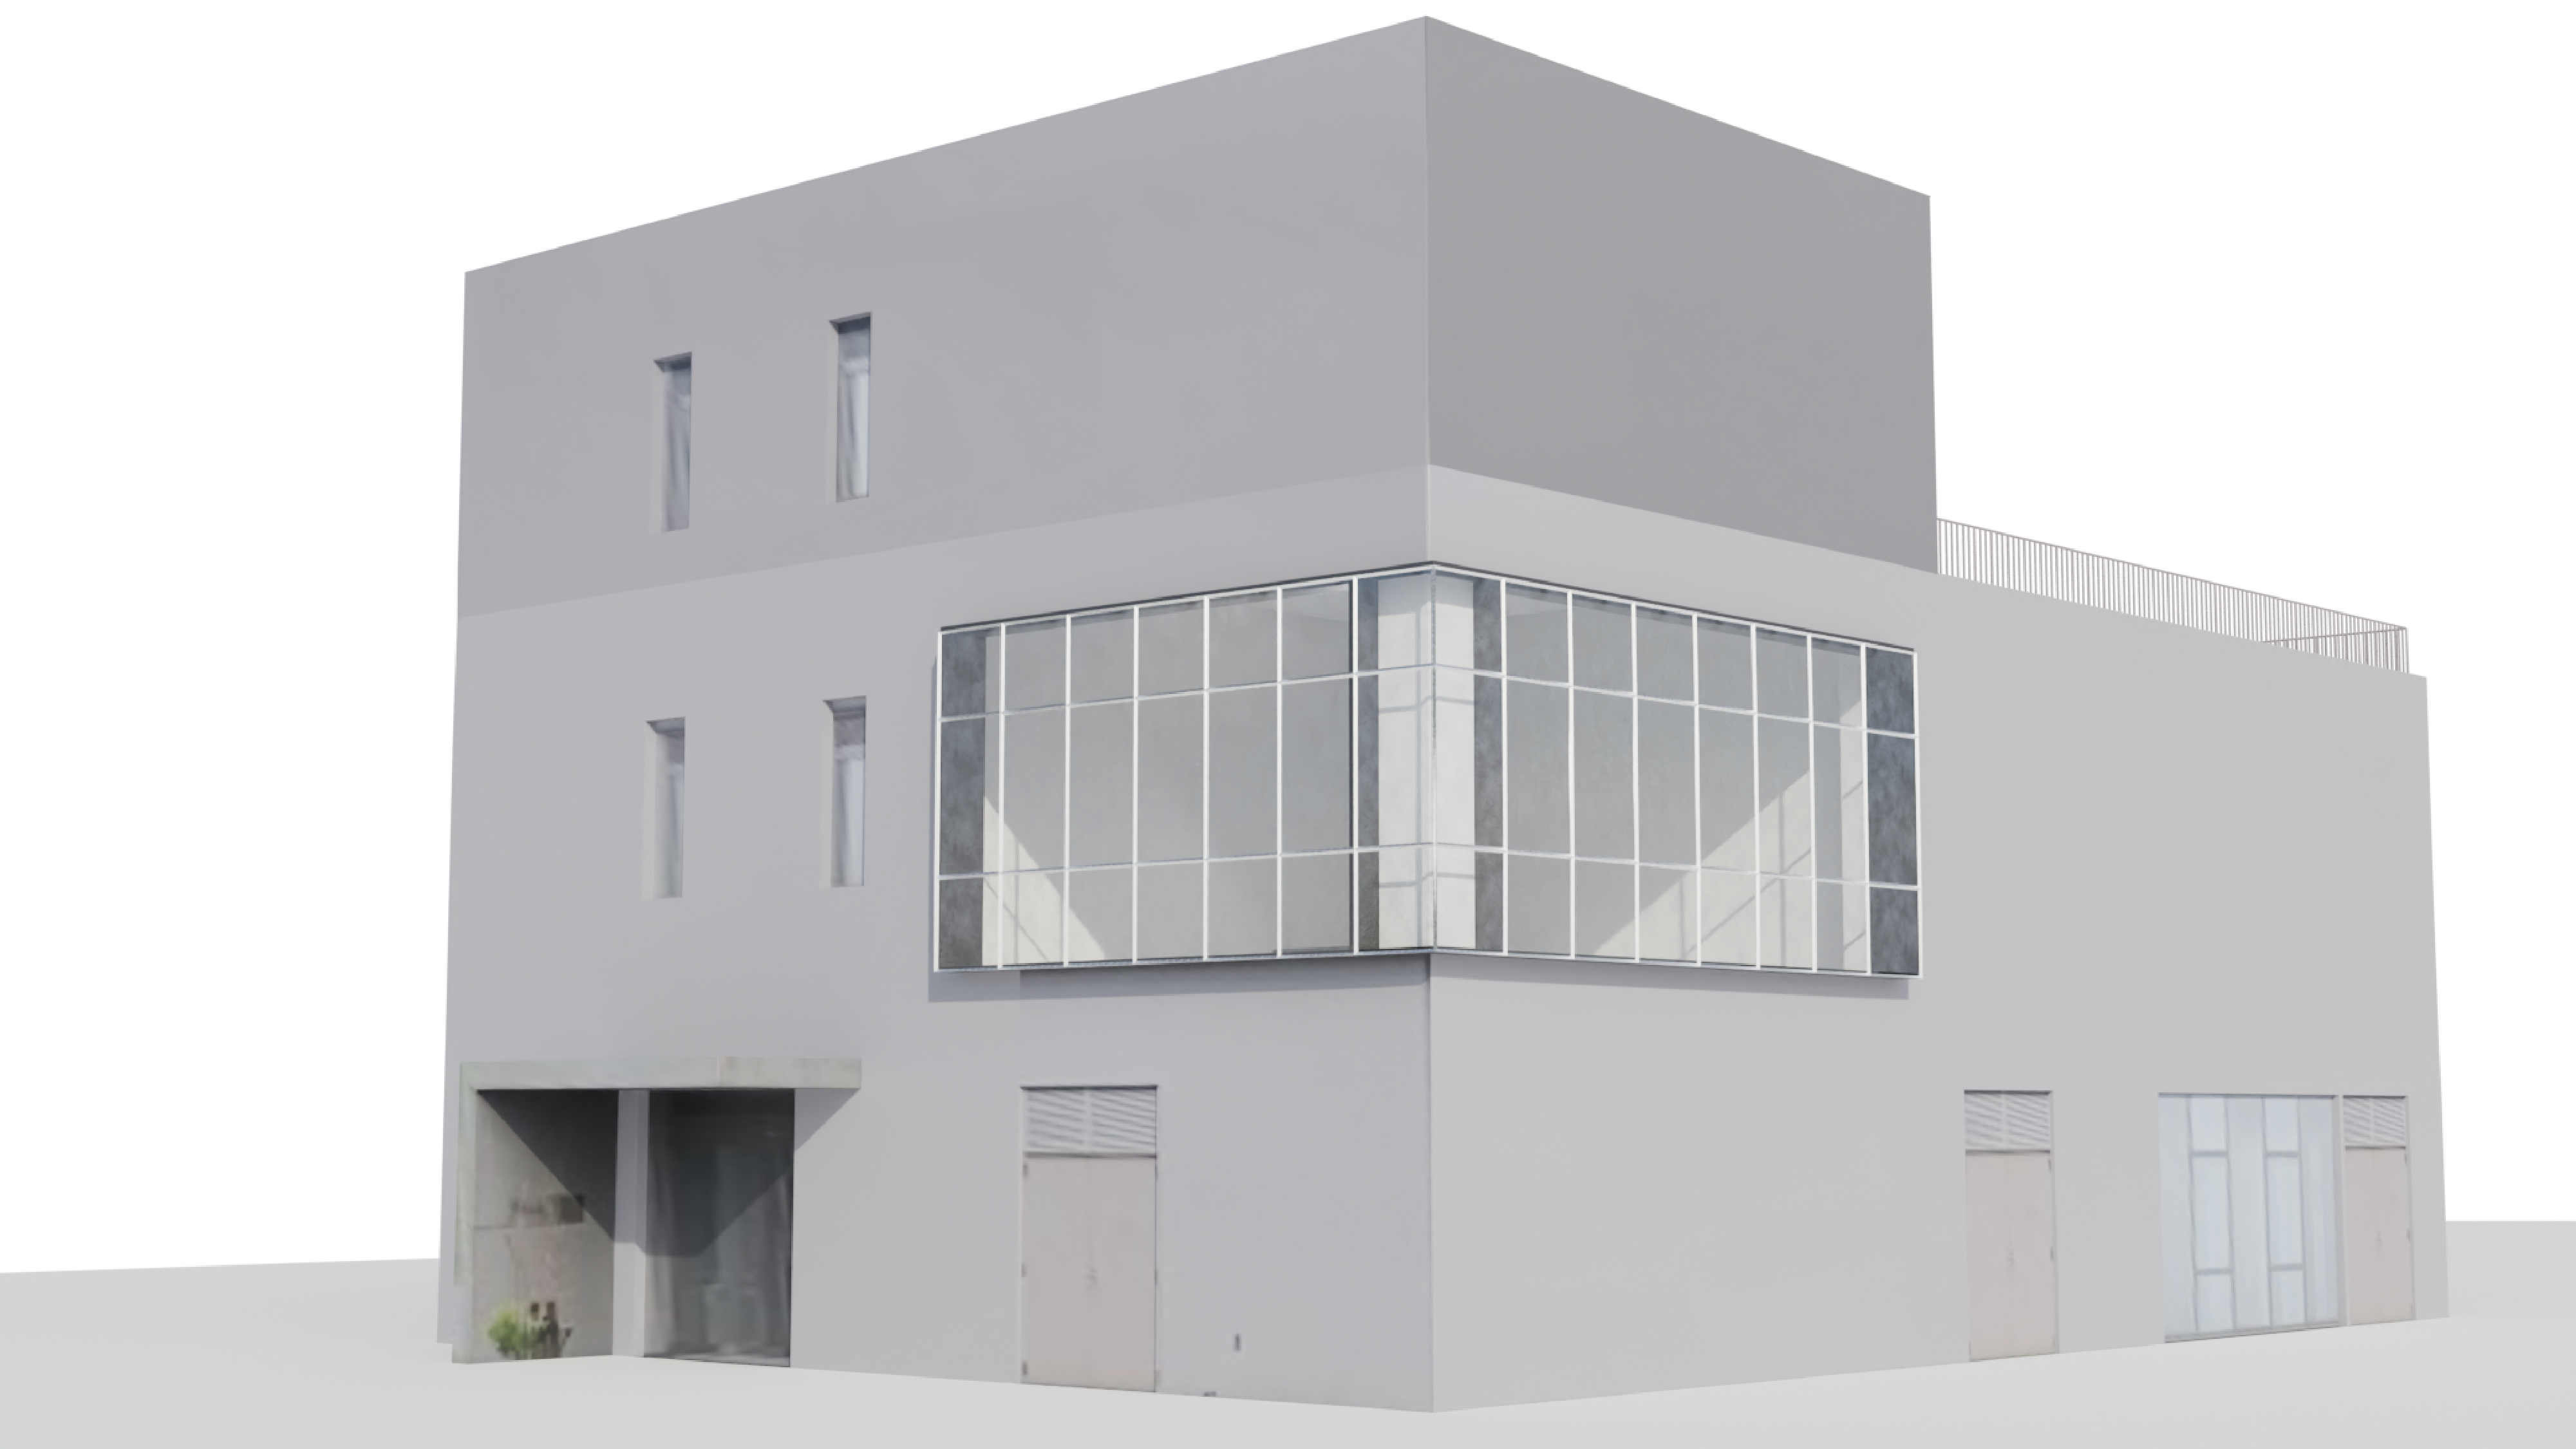
\includegraphics[width=1\linewidth]{Images/Base Module/Building}} &
              {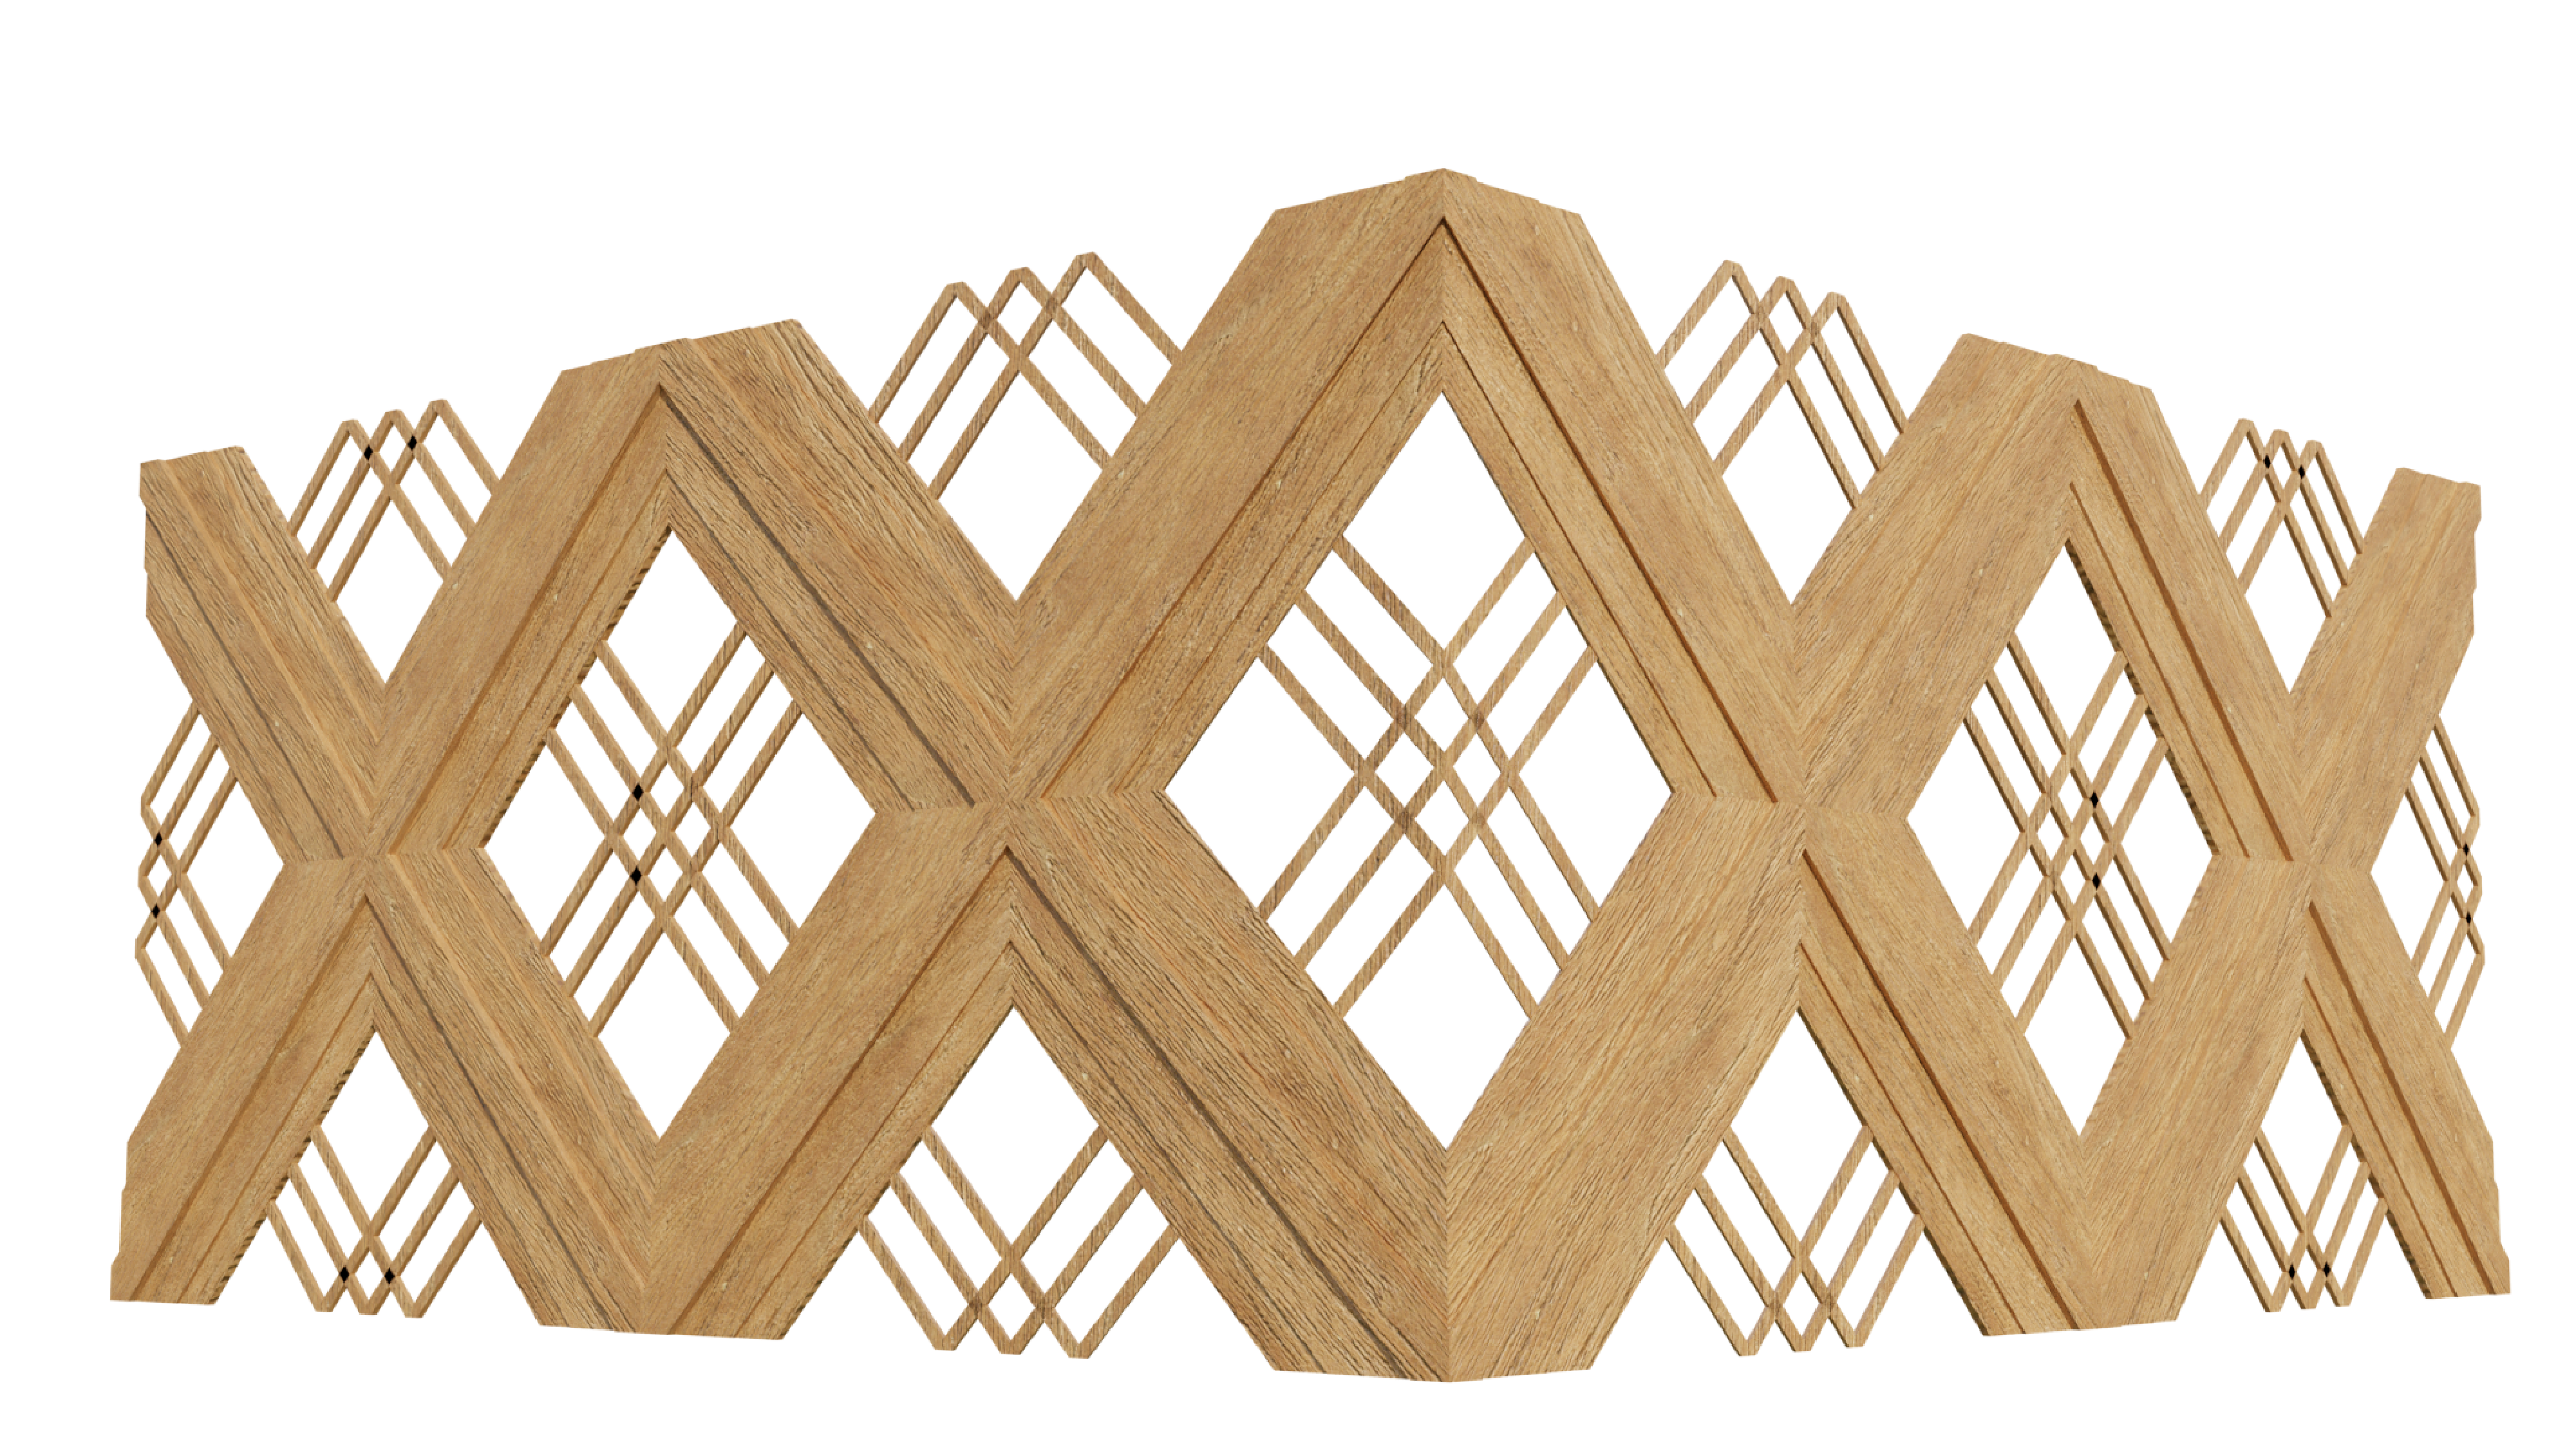
\includegraphics[width=1\linewidth]{Images/Base Module/Pattern1}} &
              {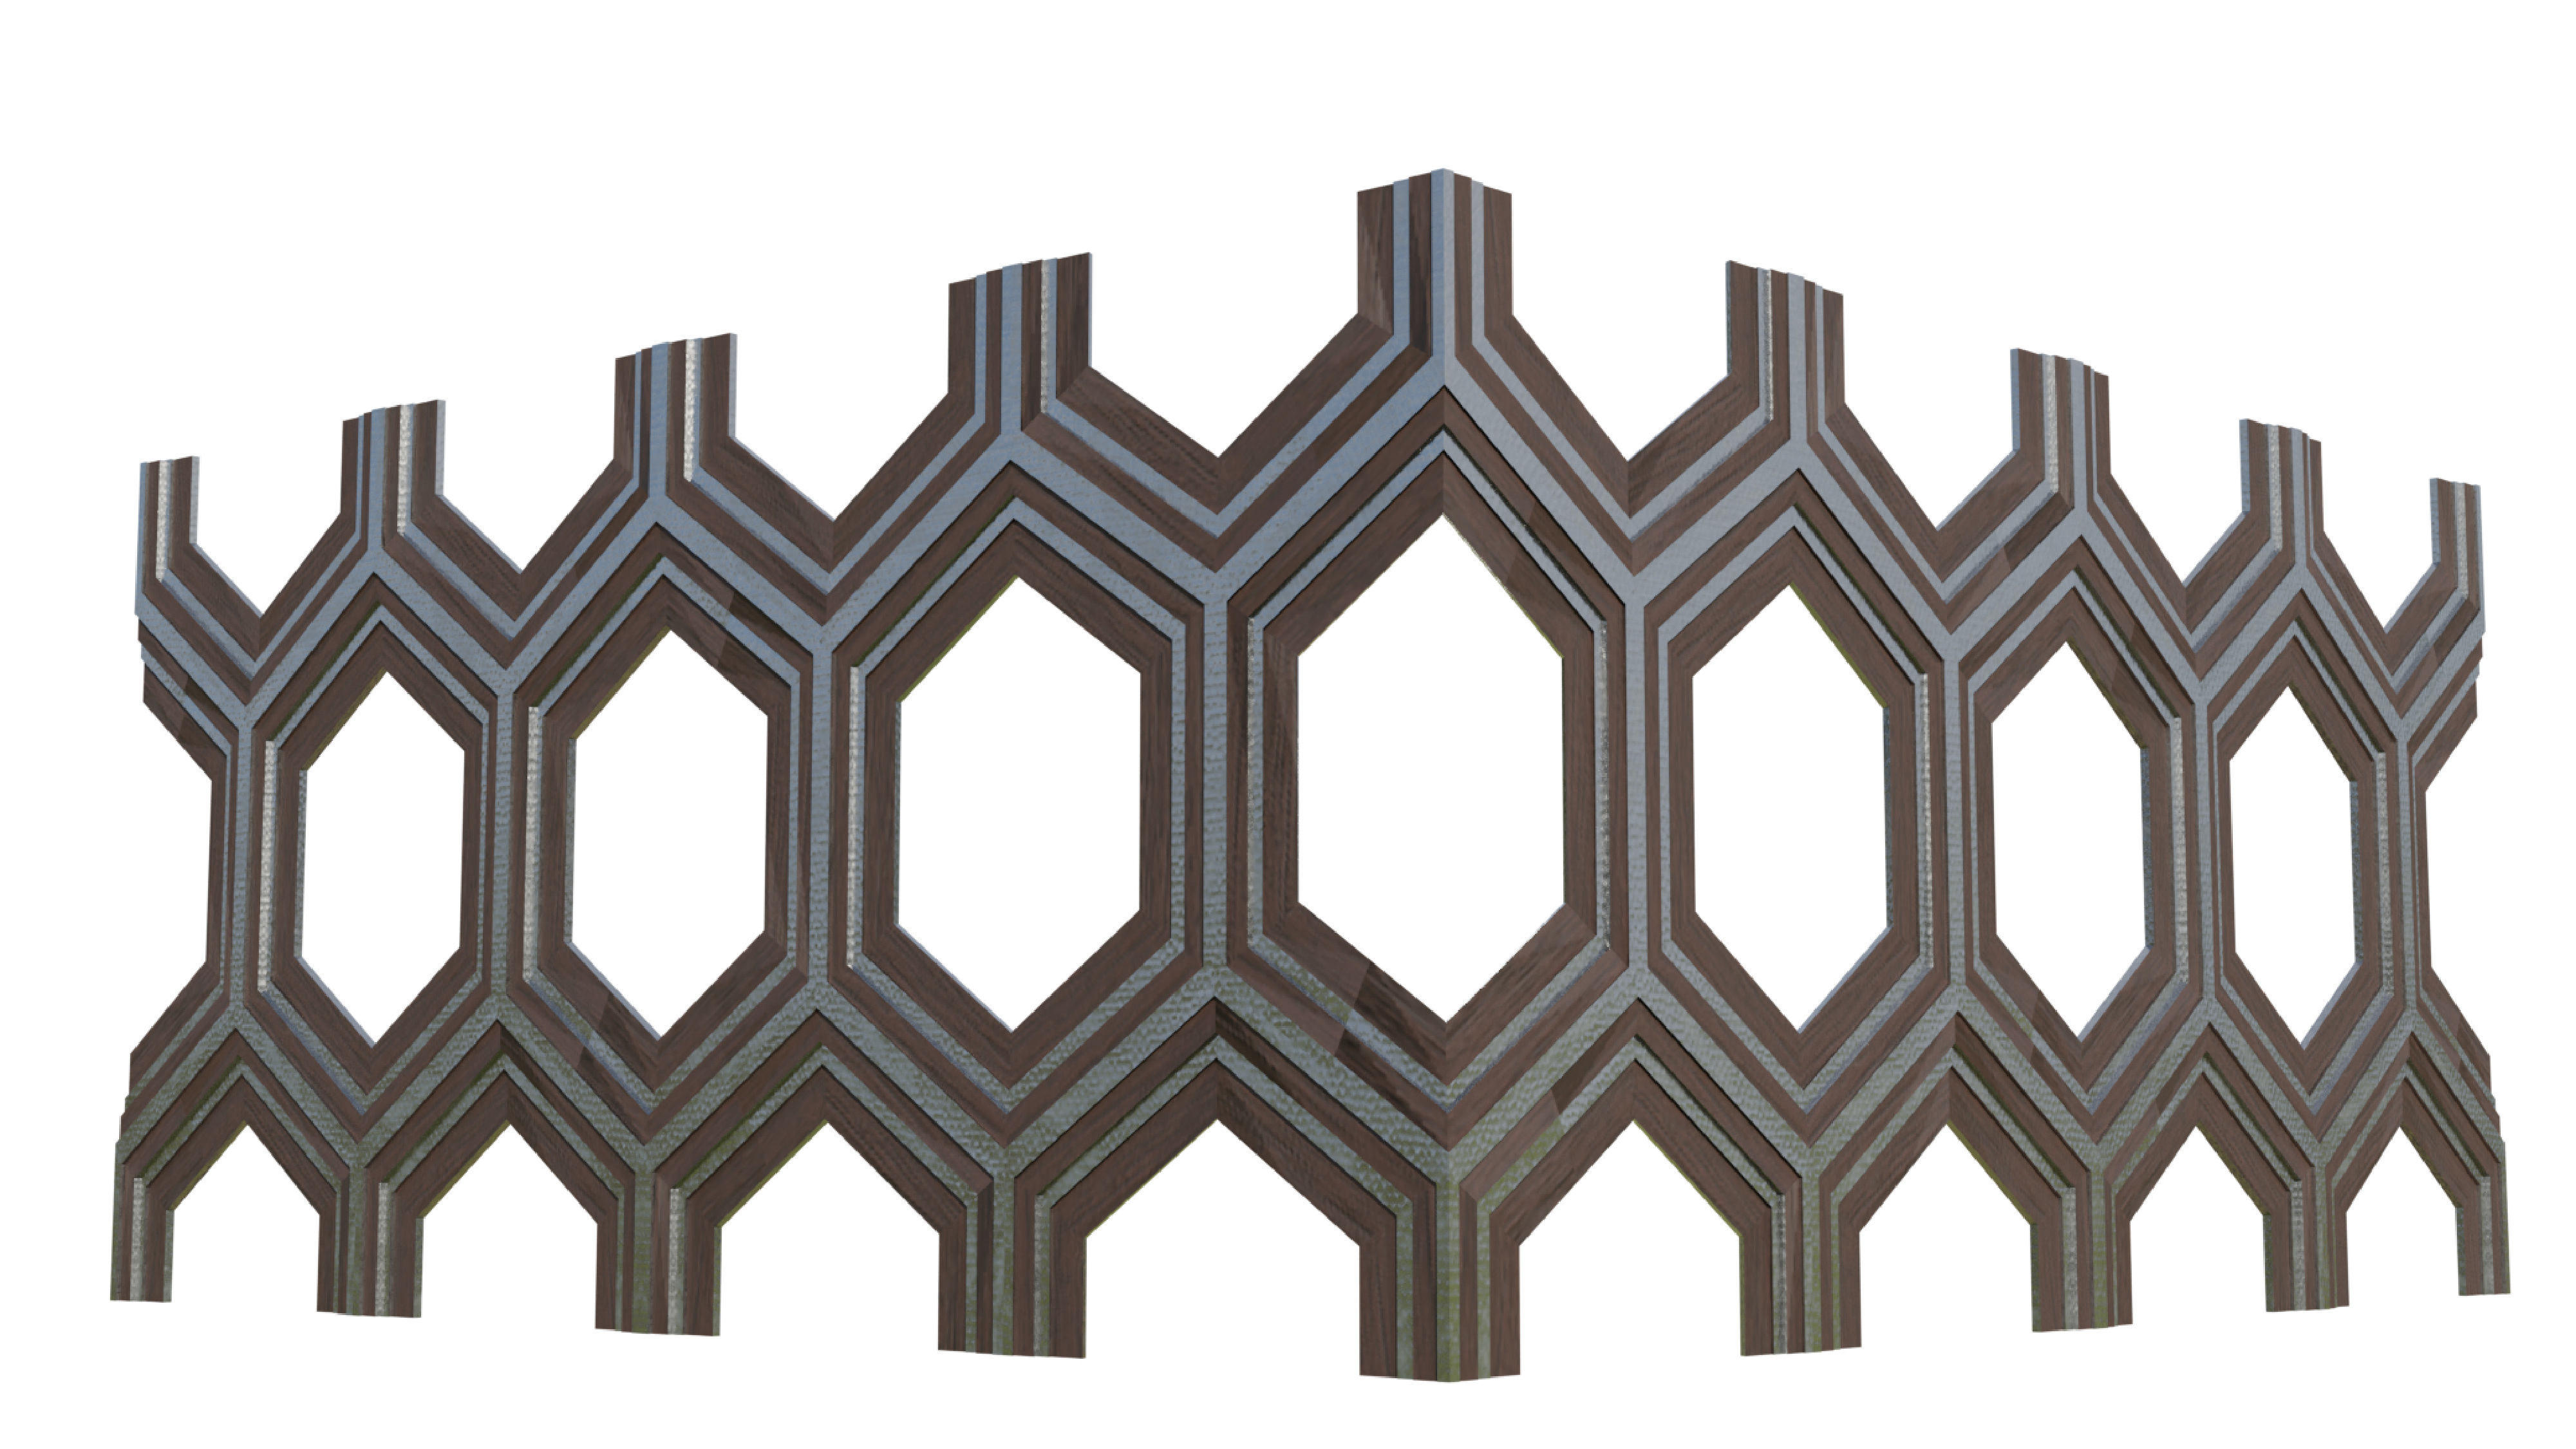
\includegraphics[width=1\linewidth]{Images/Base Module/Pattern2}} &
              {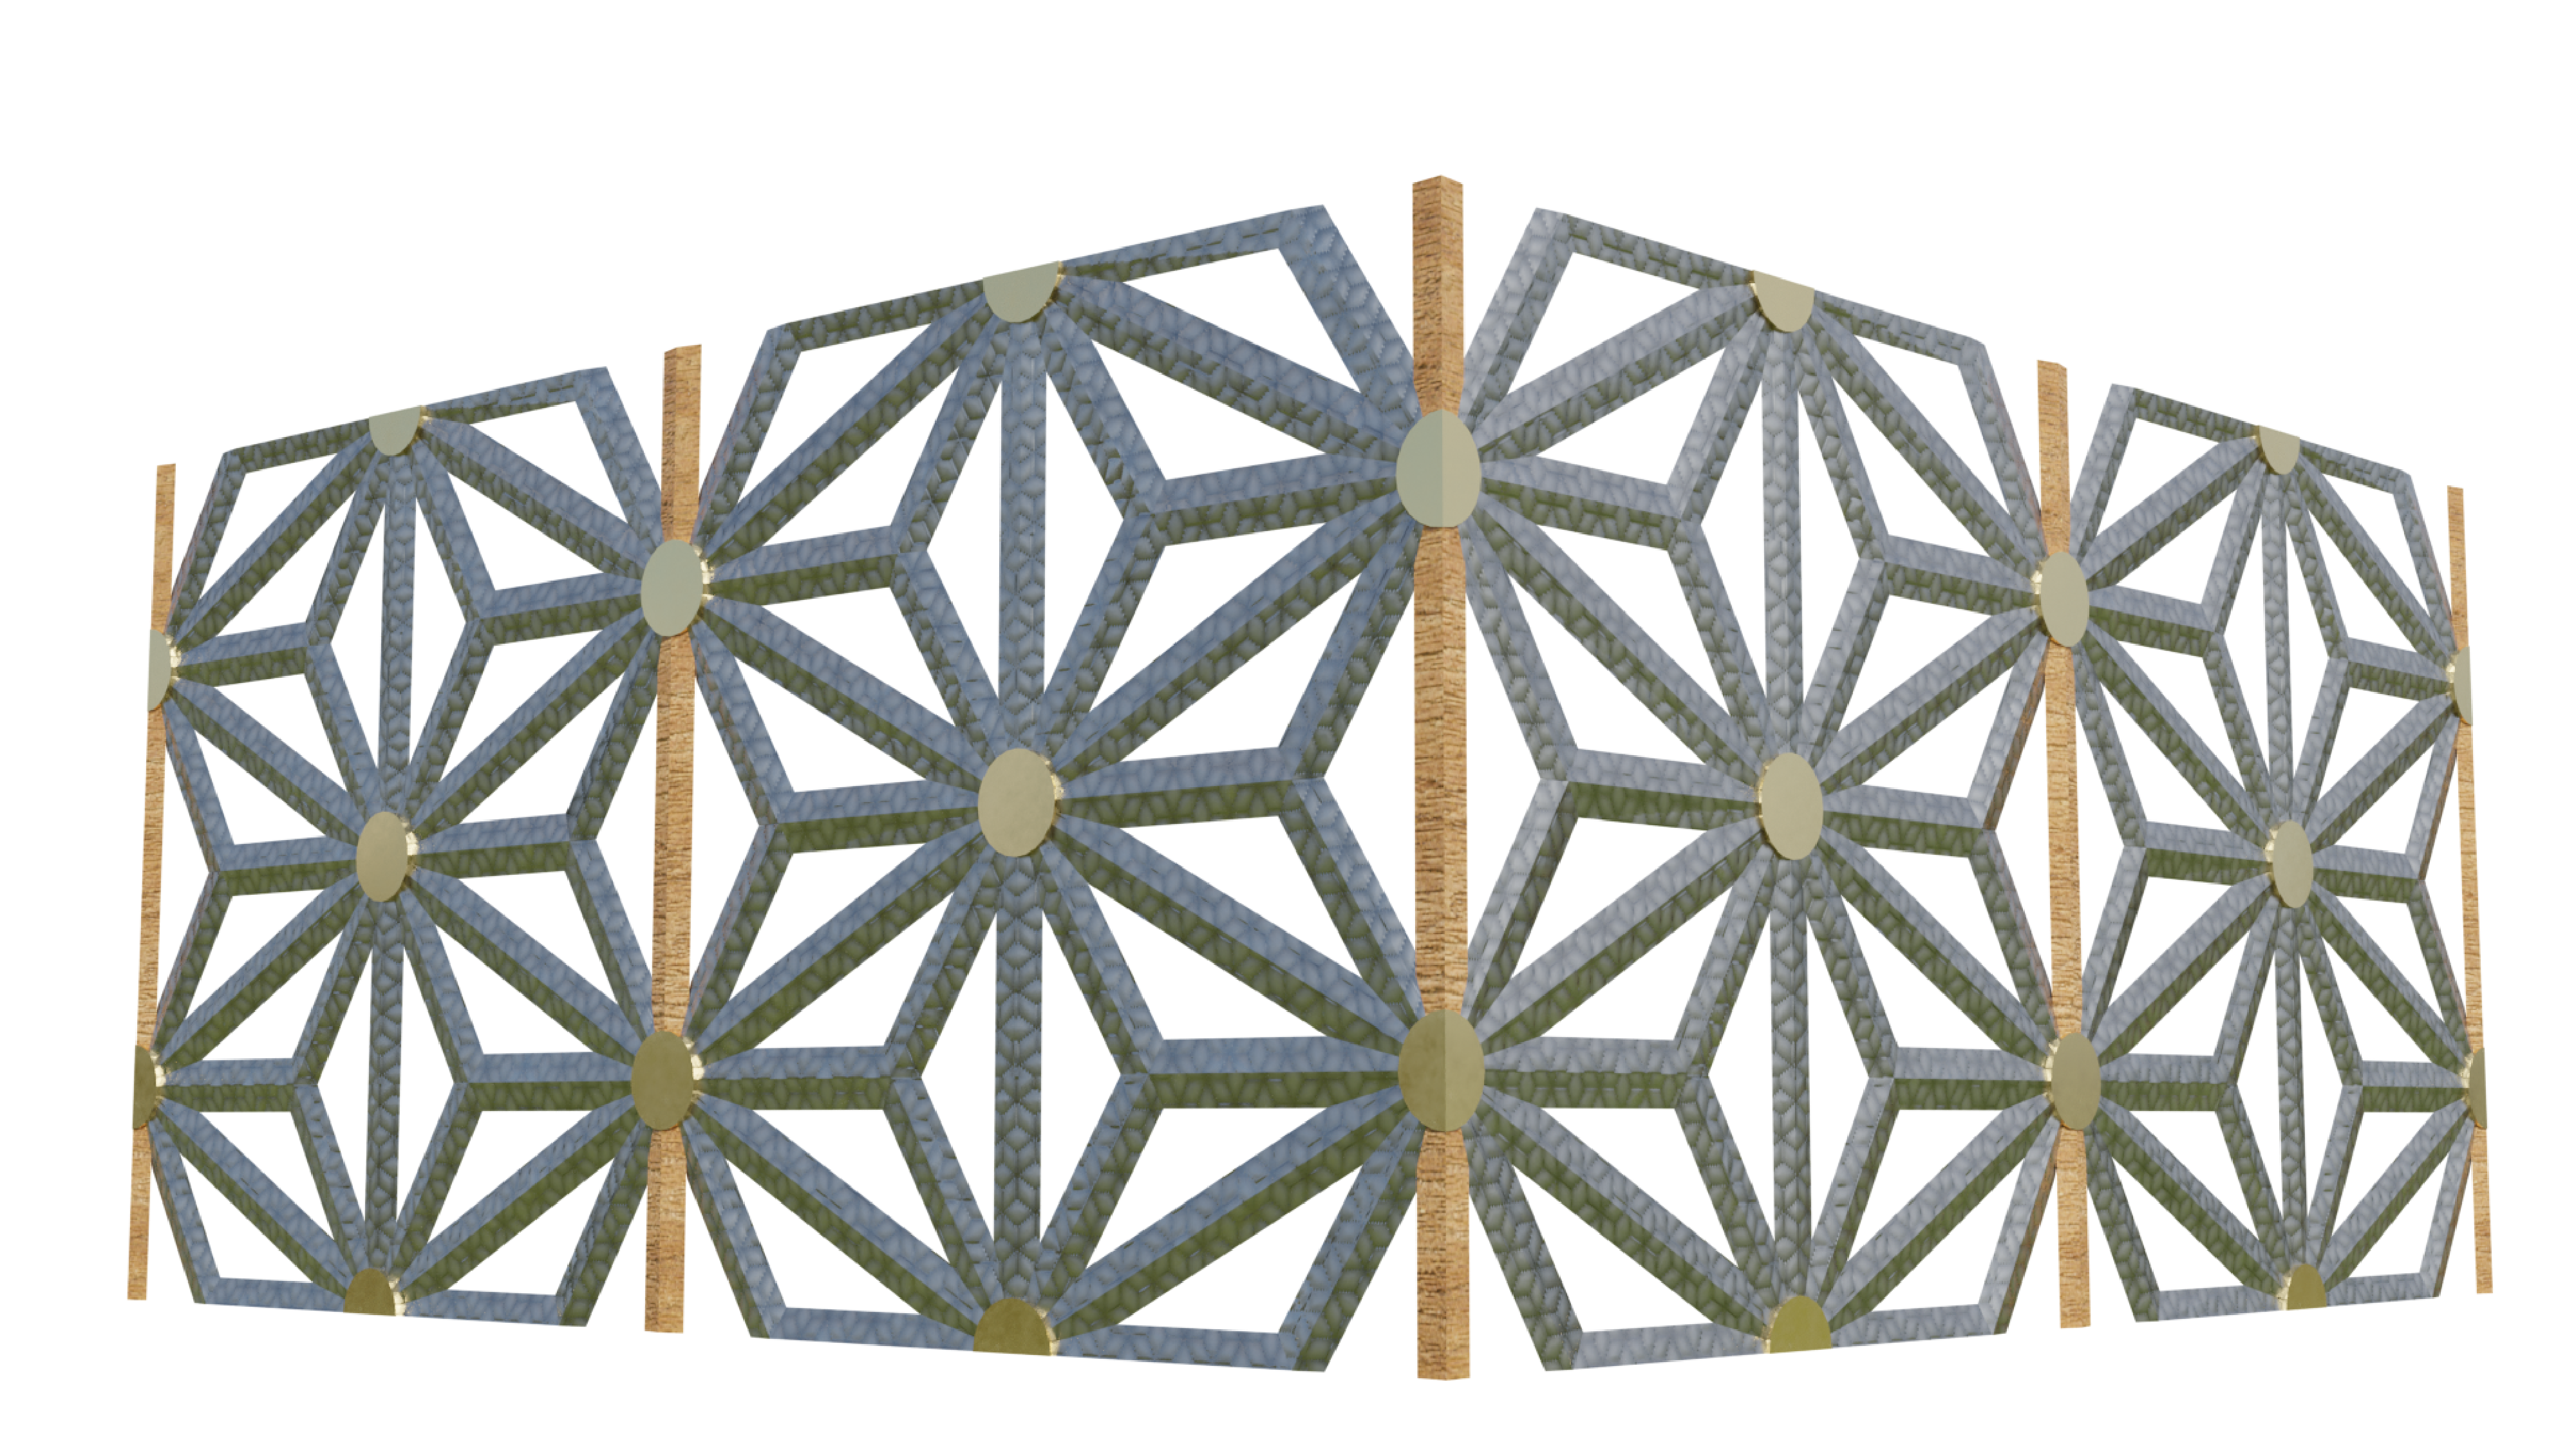
\includegraphics[width=1\linewidth]{Images/Base Module/Pattern3}} \\

            \midrule
            \textit{Mesh per complexity Level} &
              \textit{Pattern 1} &
              \textit{Pattern 2} &
              \textit{Pattern 3}\\

            \midrule
            \text{Level 3} &  &  &
            \\
            {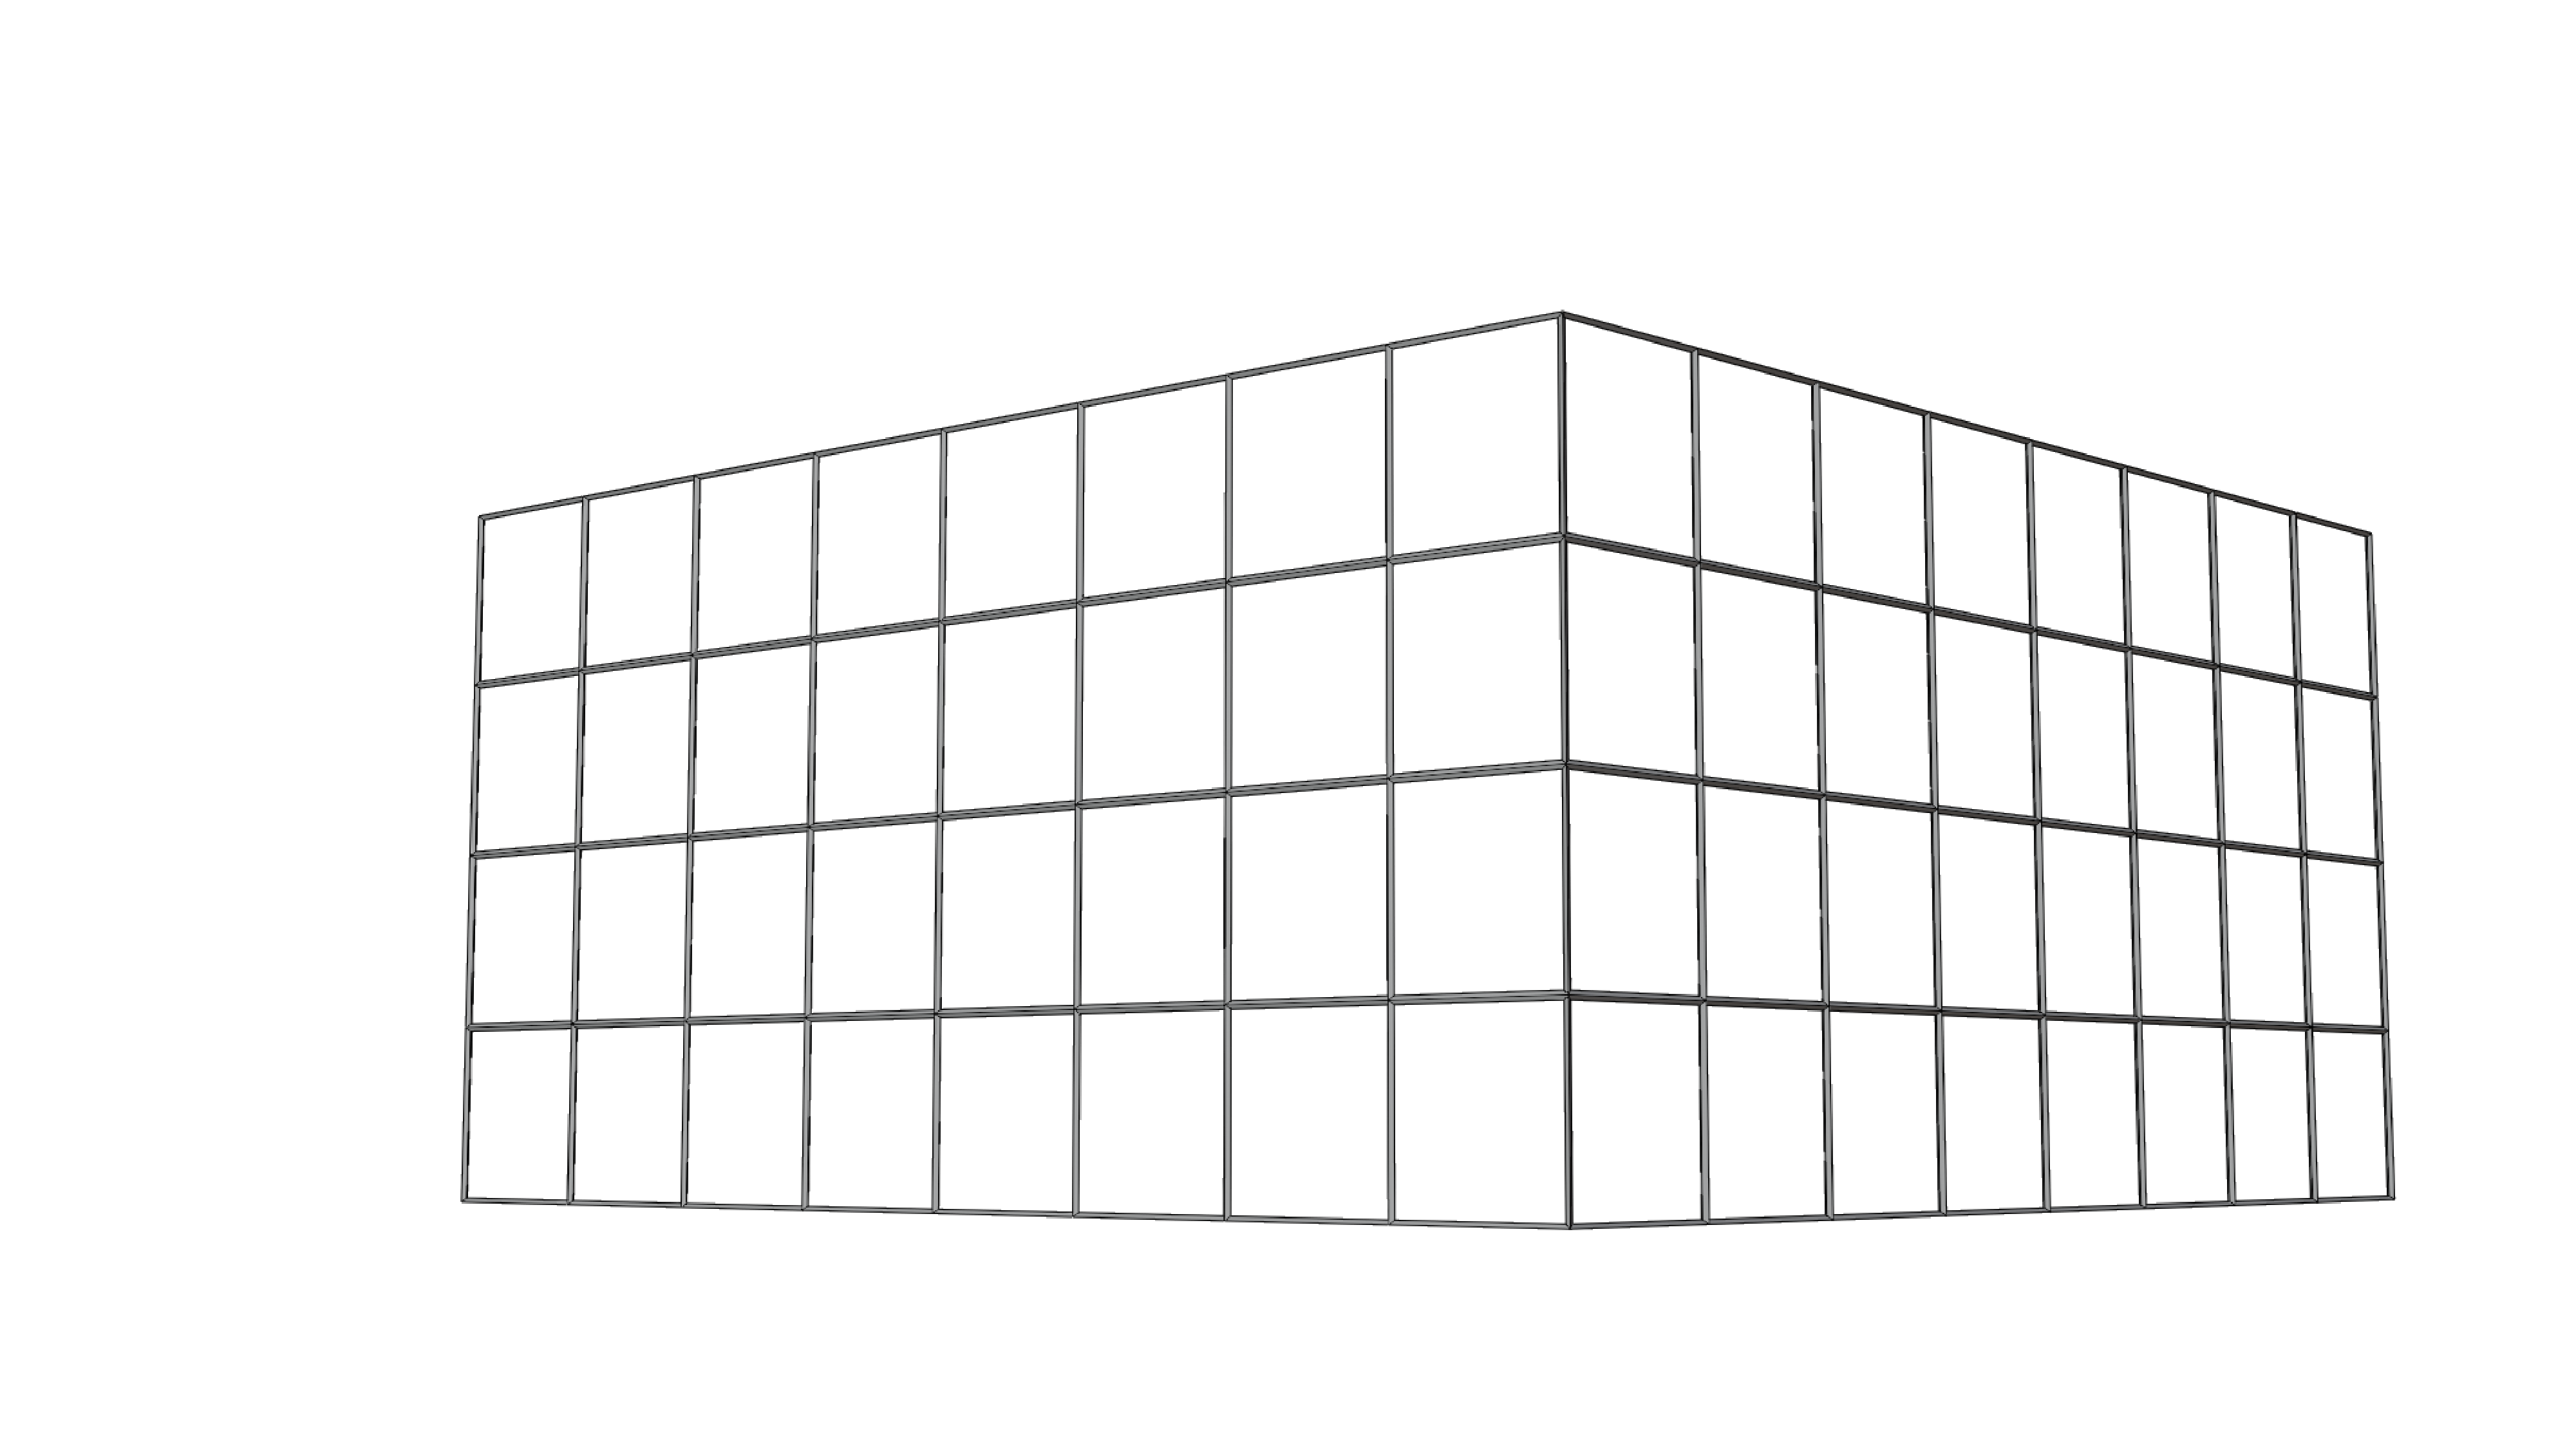
\includegraphics[width=1\linewidth]{Images/Wall 0/0003}} &
              {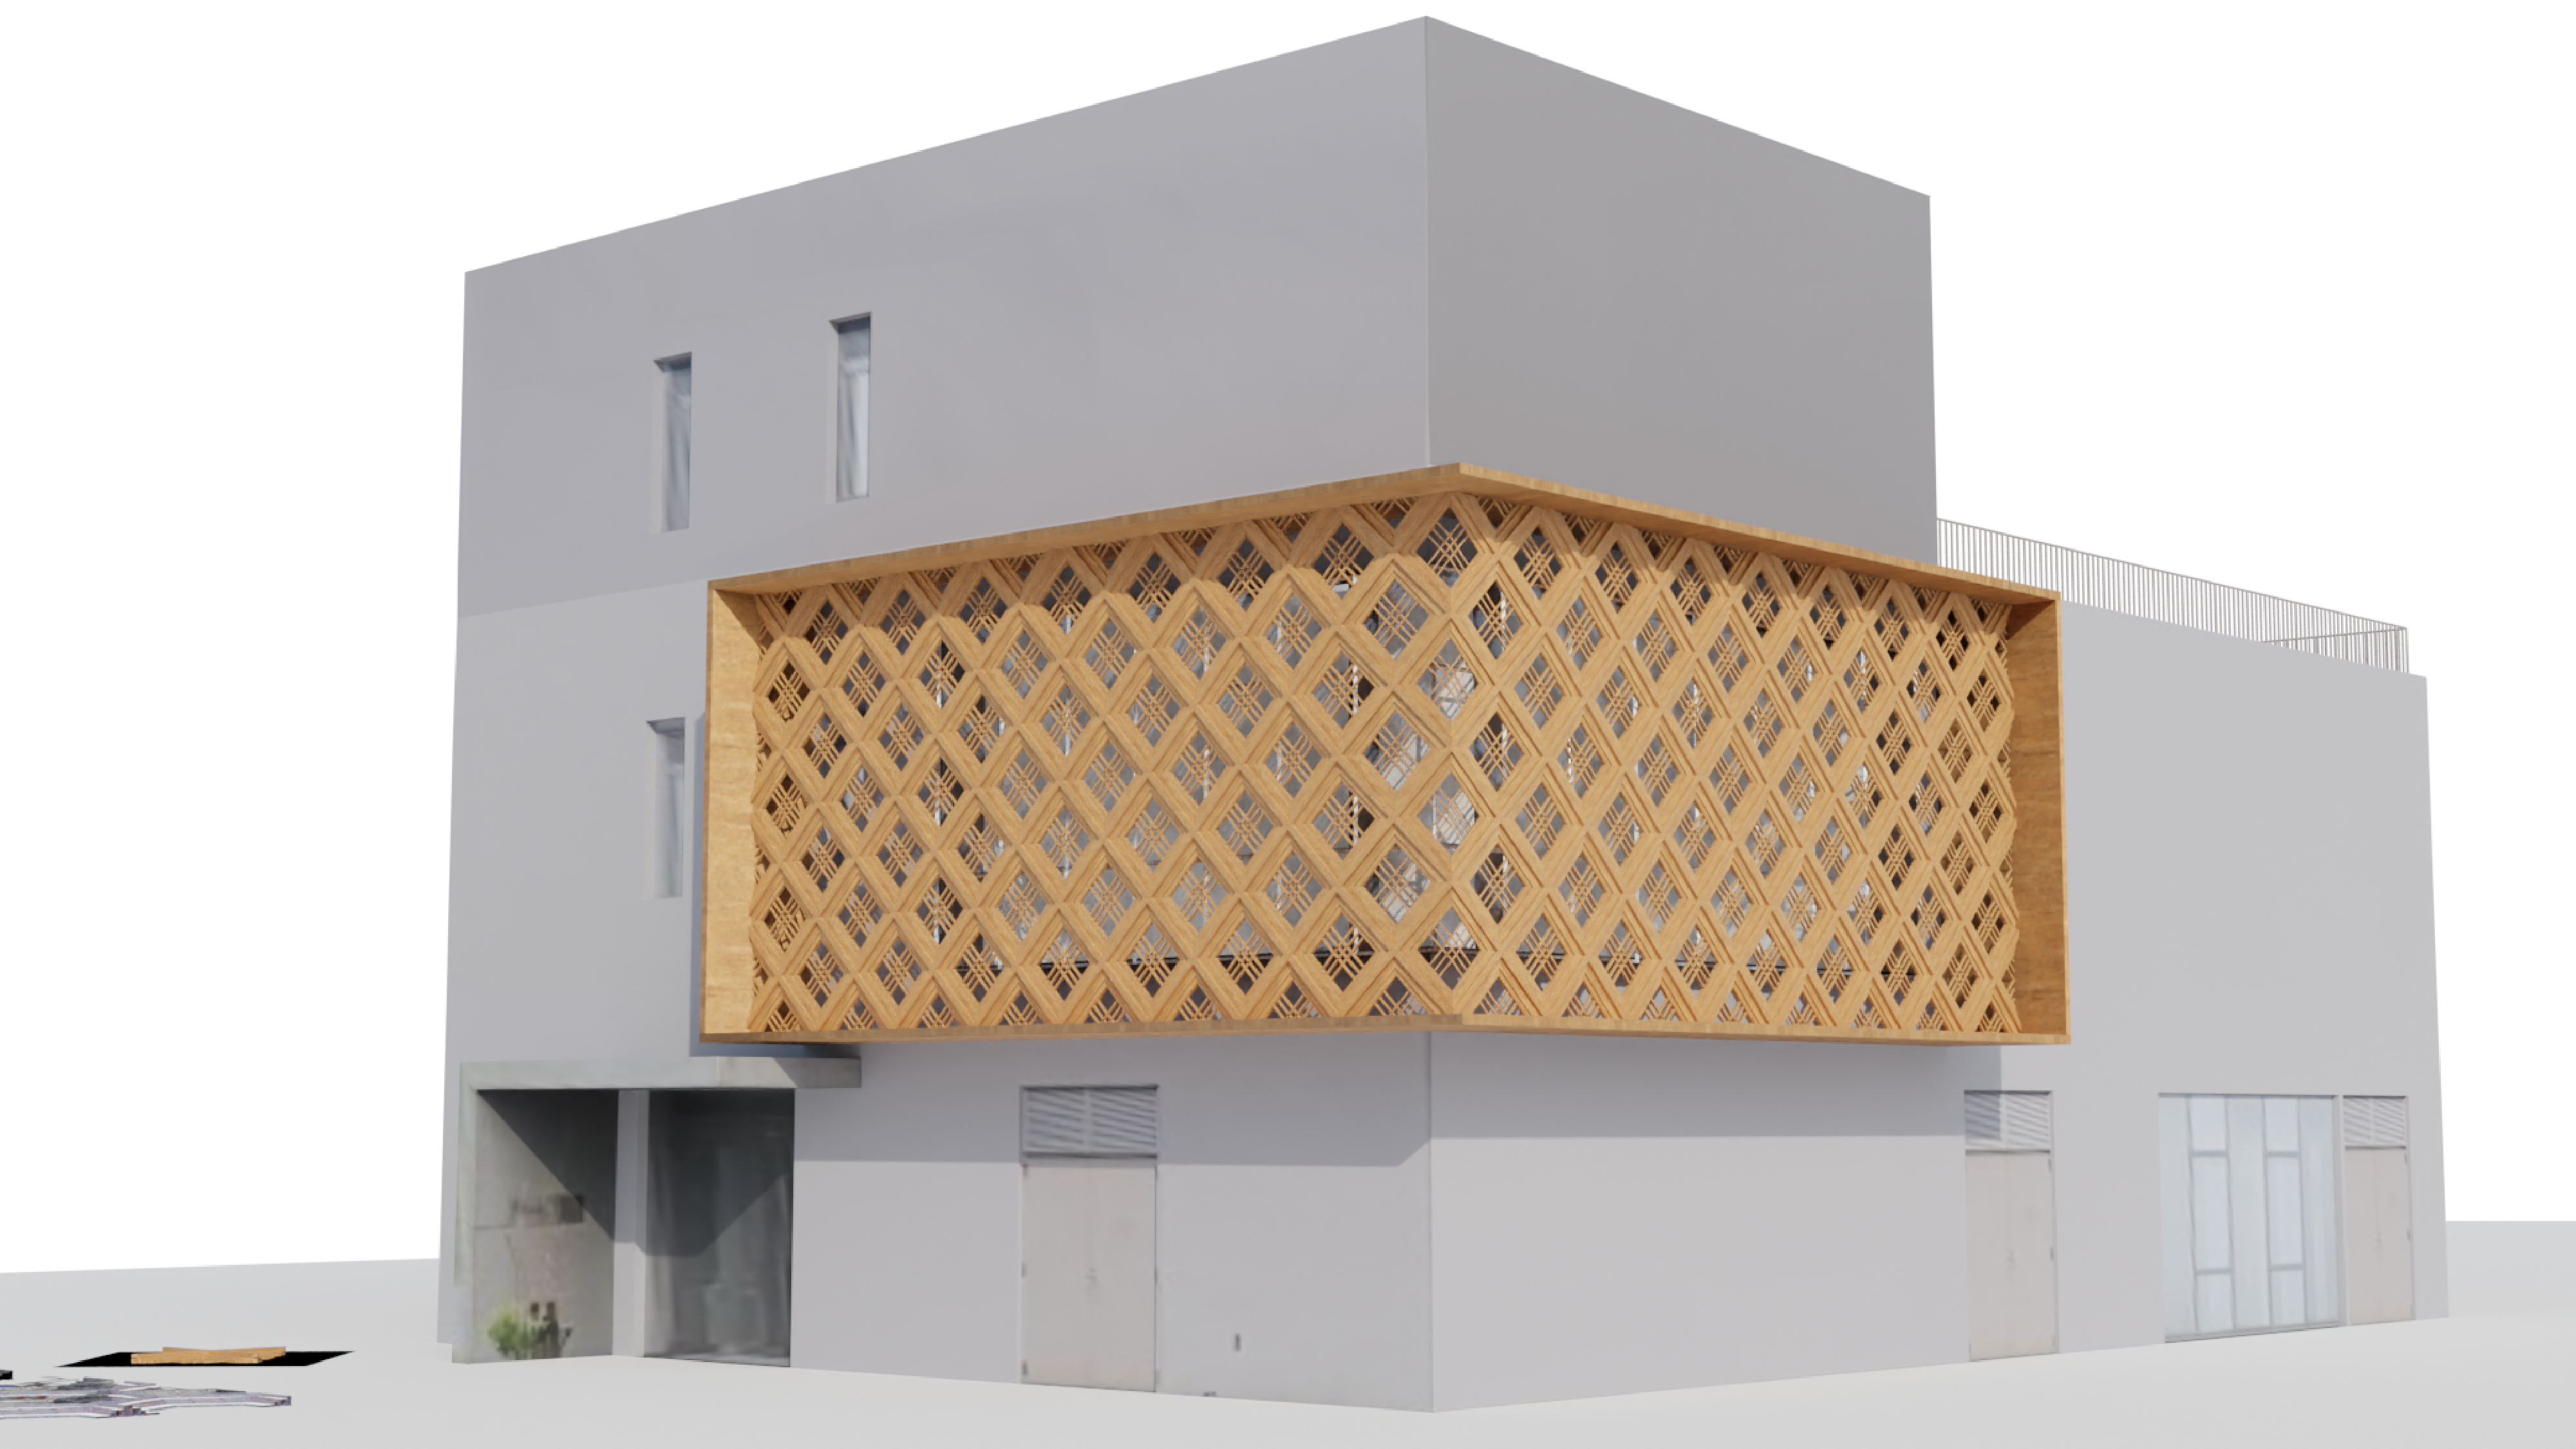
\includegraphics[width=1\linewidth]{Images/Pattern 1/0003}} &
              {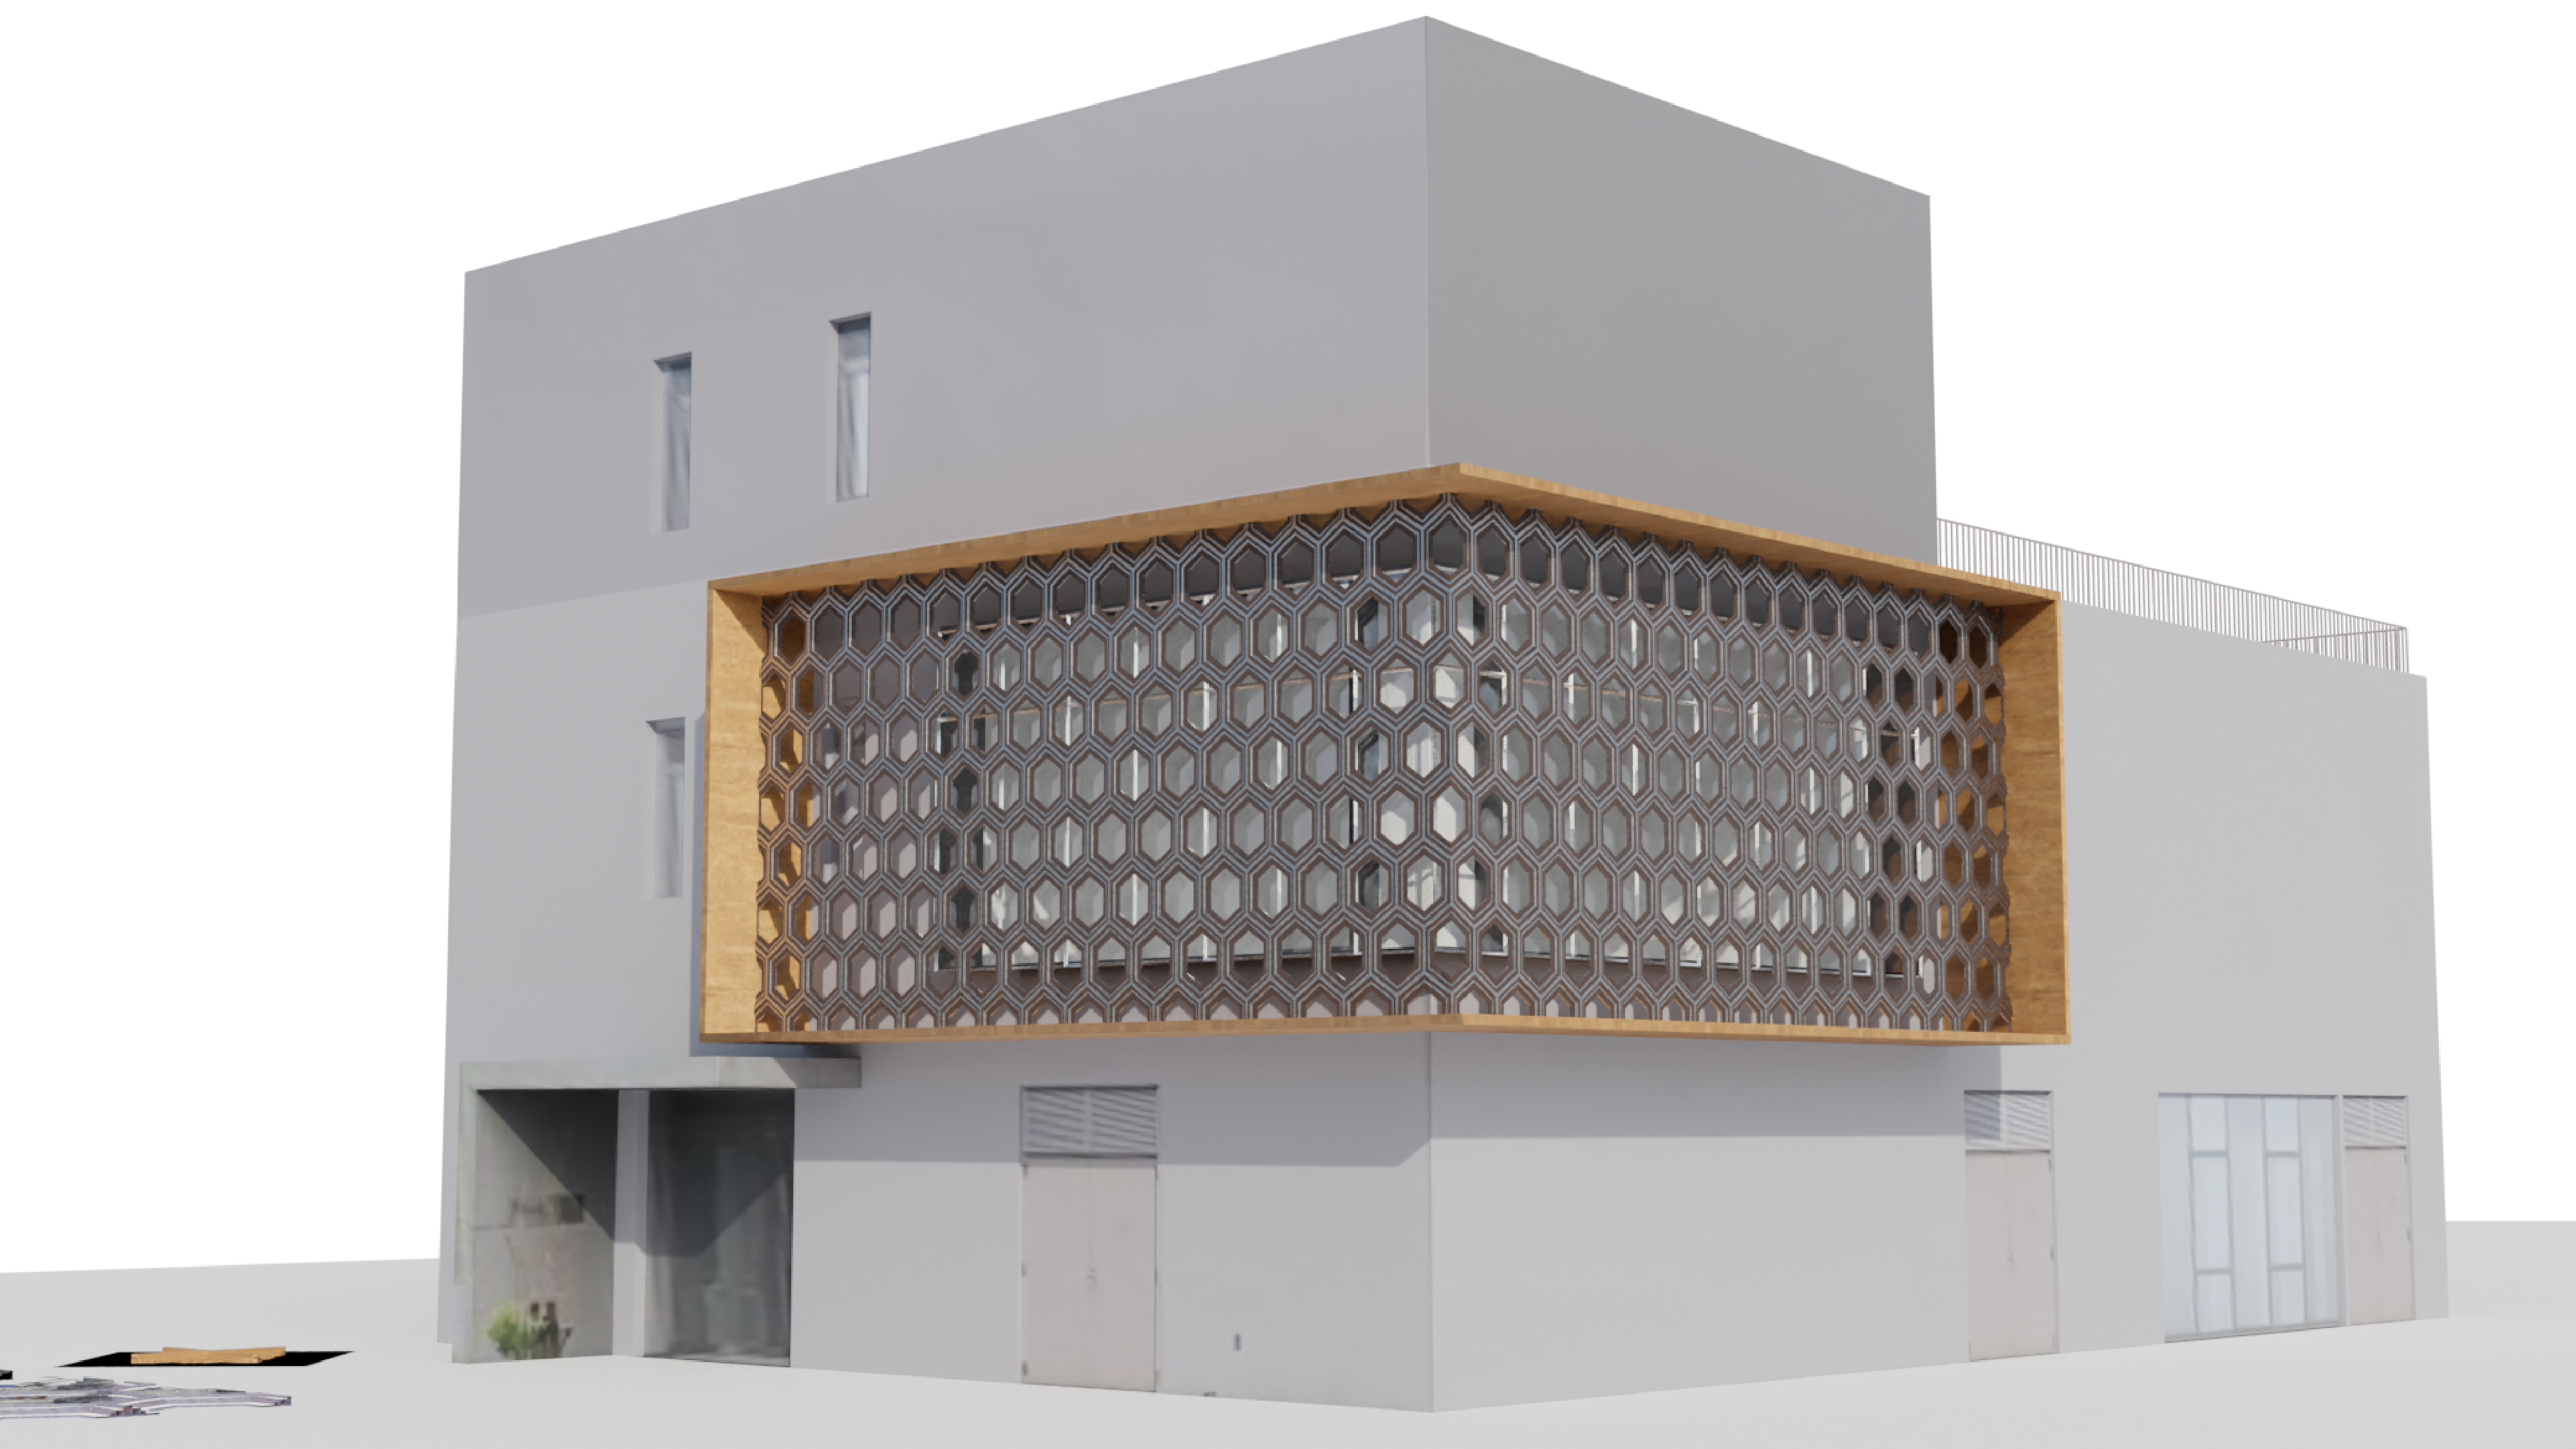
\includegraphics[width=1\linewidth]{Images/Pattern 2/0003}} &
              {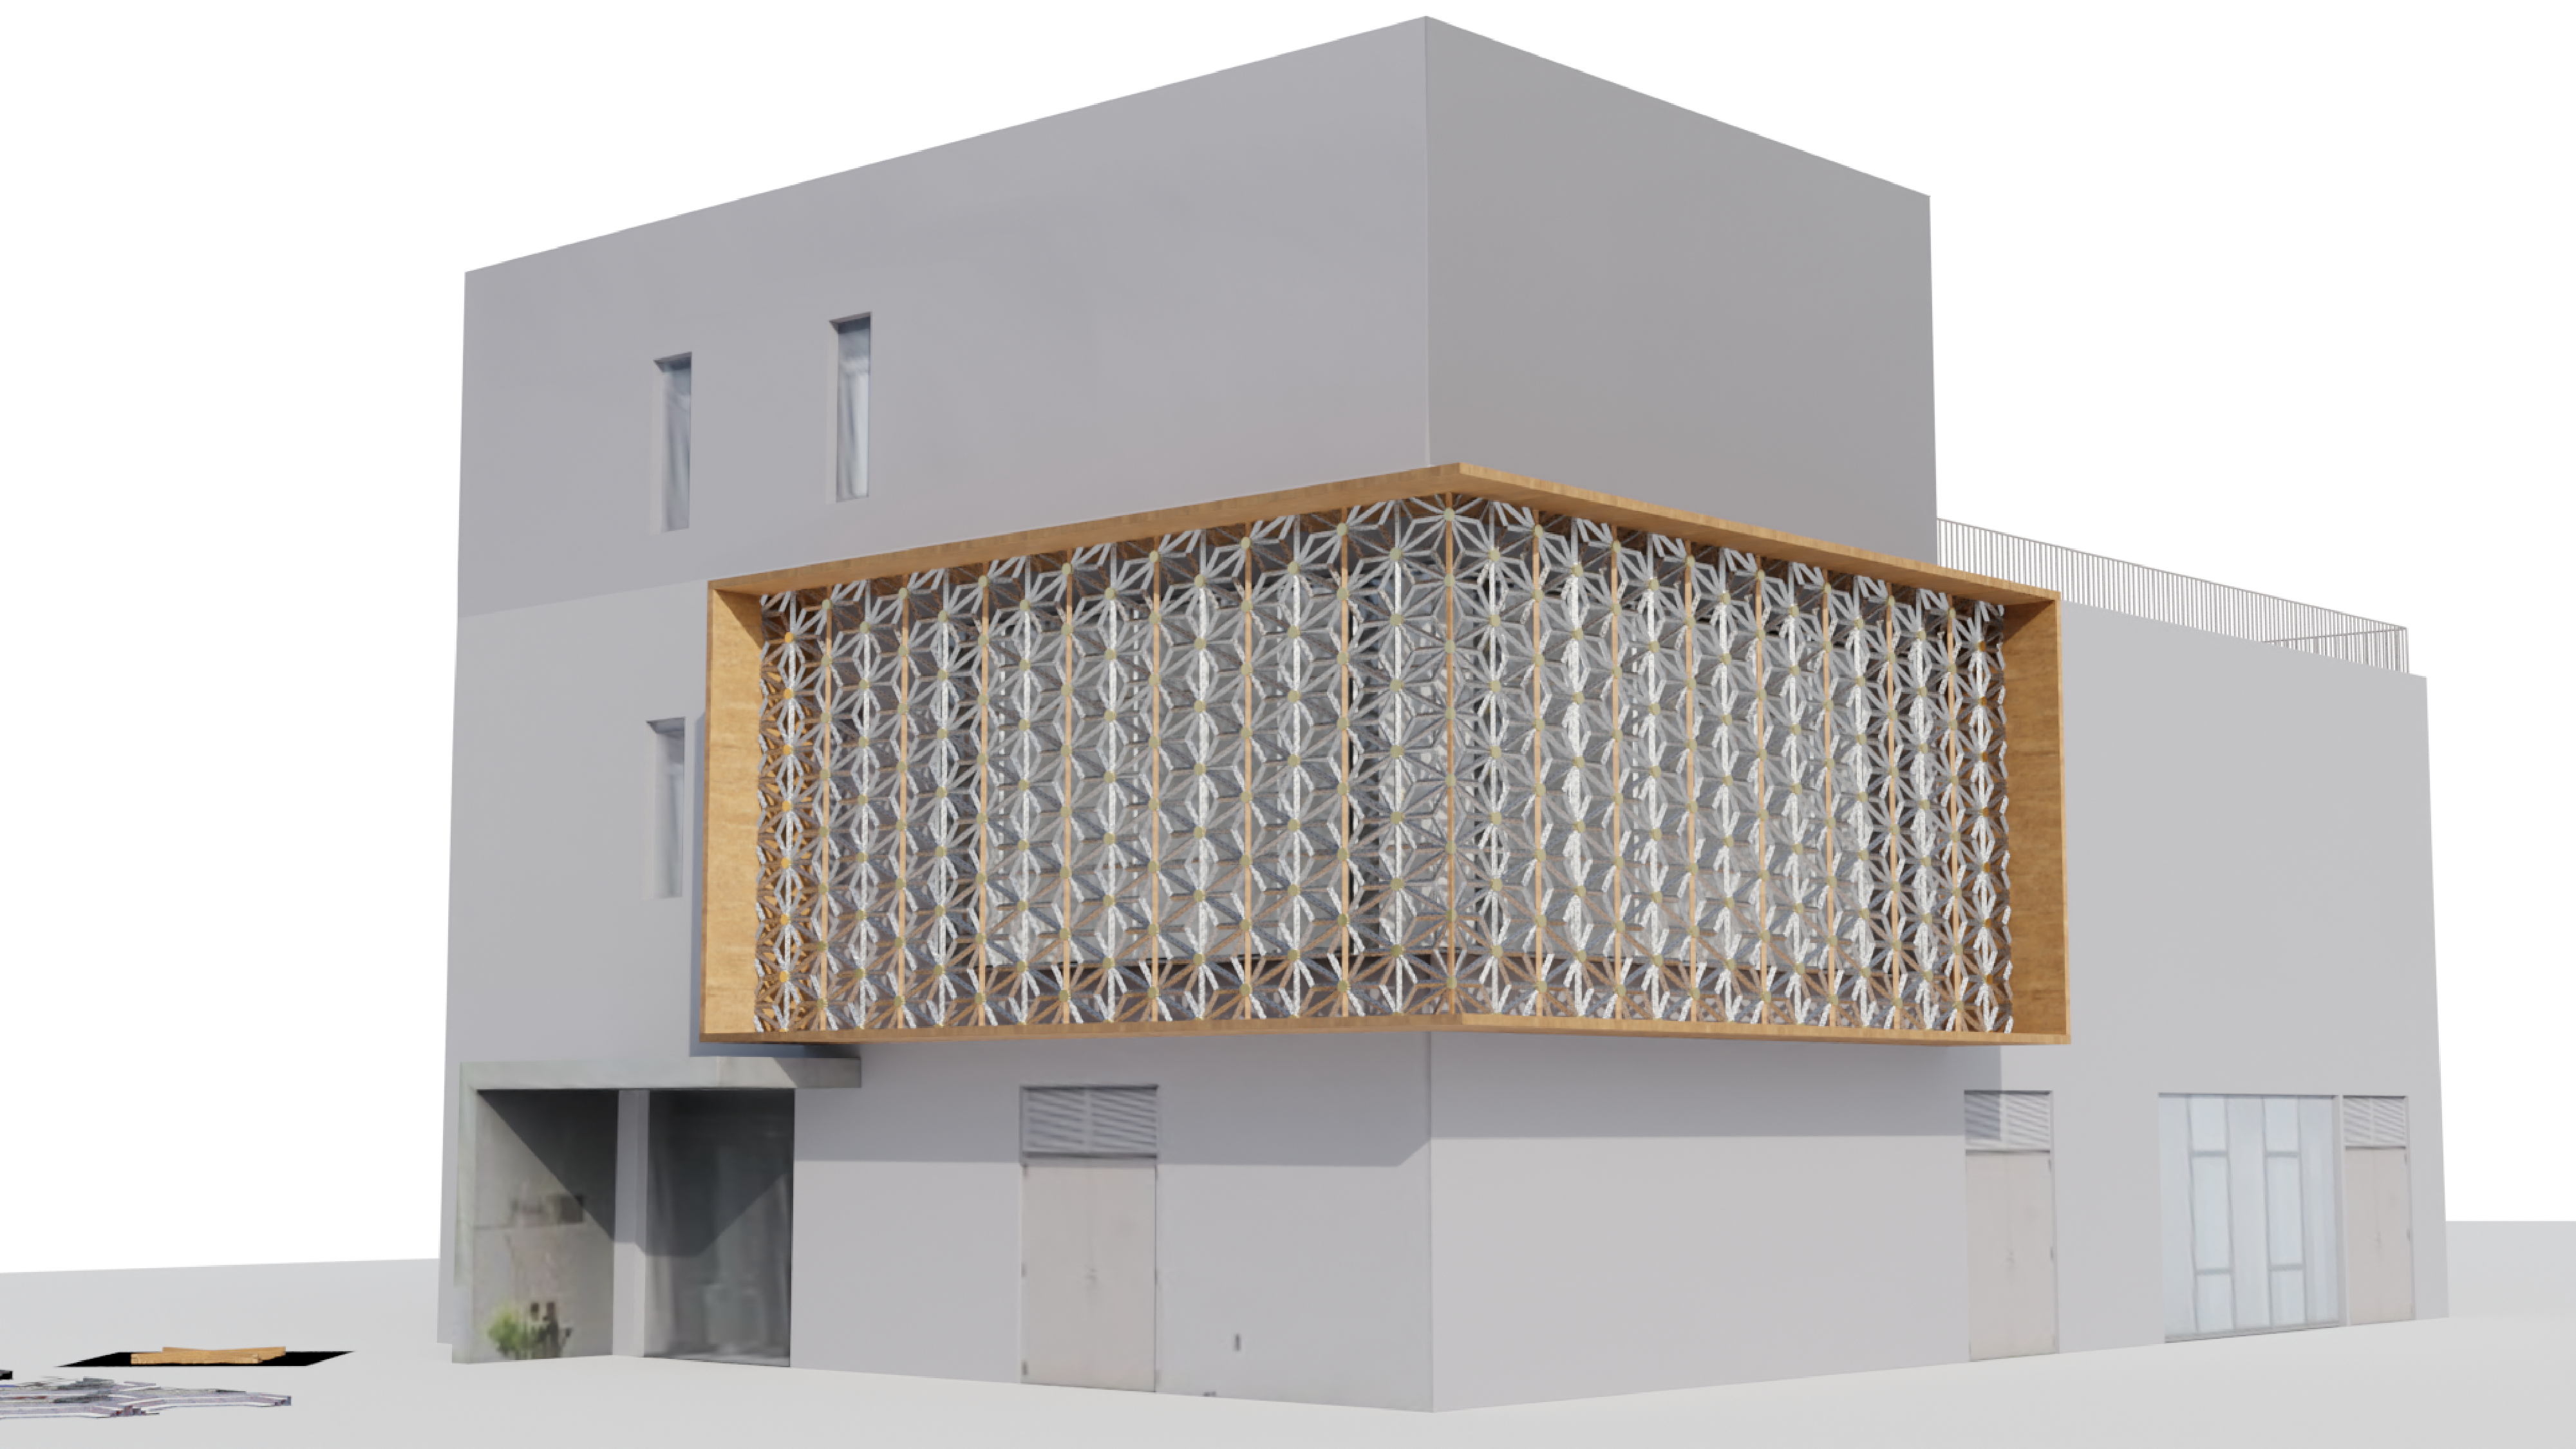
\includegraphics[width=1\linewidth]{Images/Pattern 3/0003}} \\
            \midrule
            \text{Level 6} &  &  &
            \\
            {\includegraphics[width=1\linewidth]{Images/Wall 0/0006}} &
              {\includegraphics[width=1\linewidth]{Images/Pattern 1/0006}} &
              {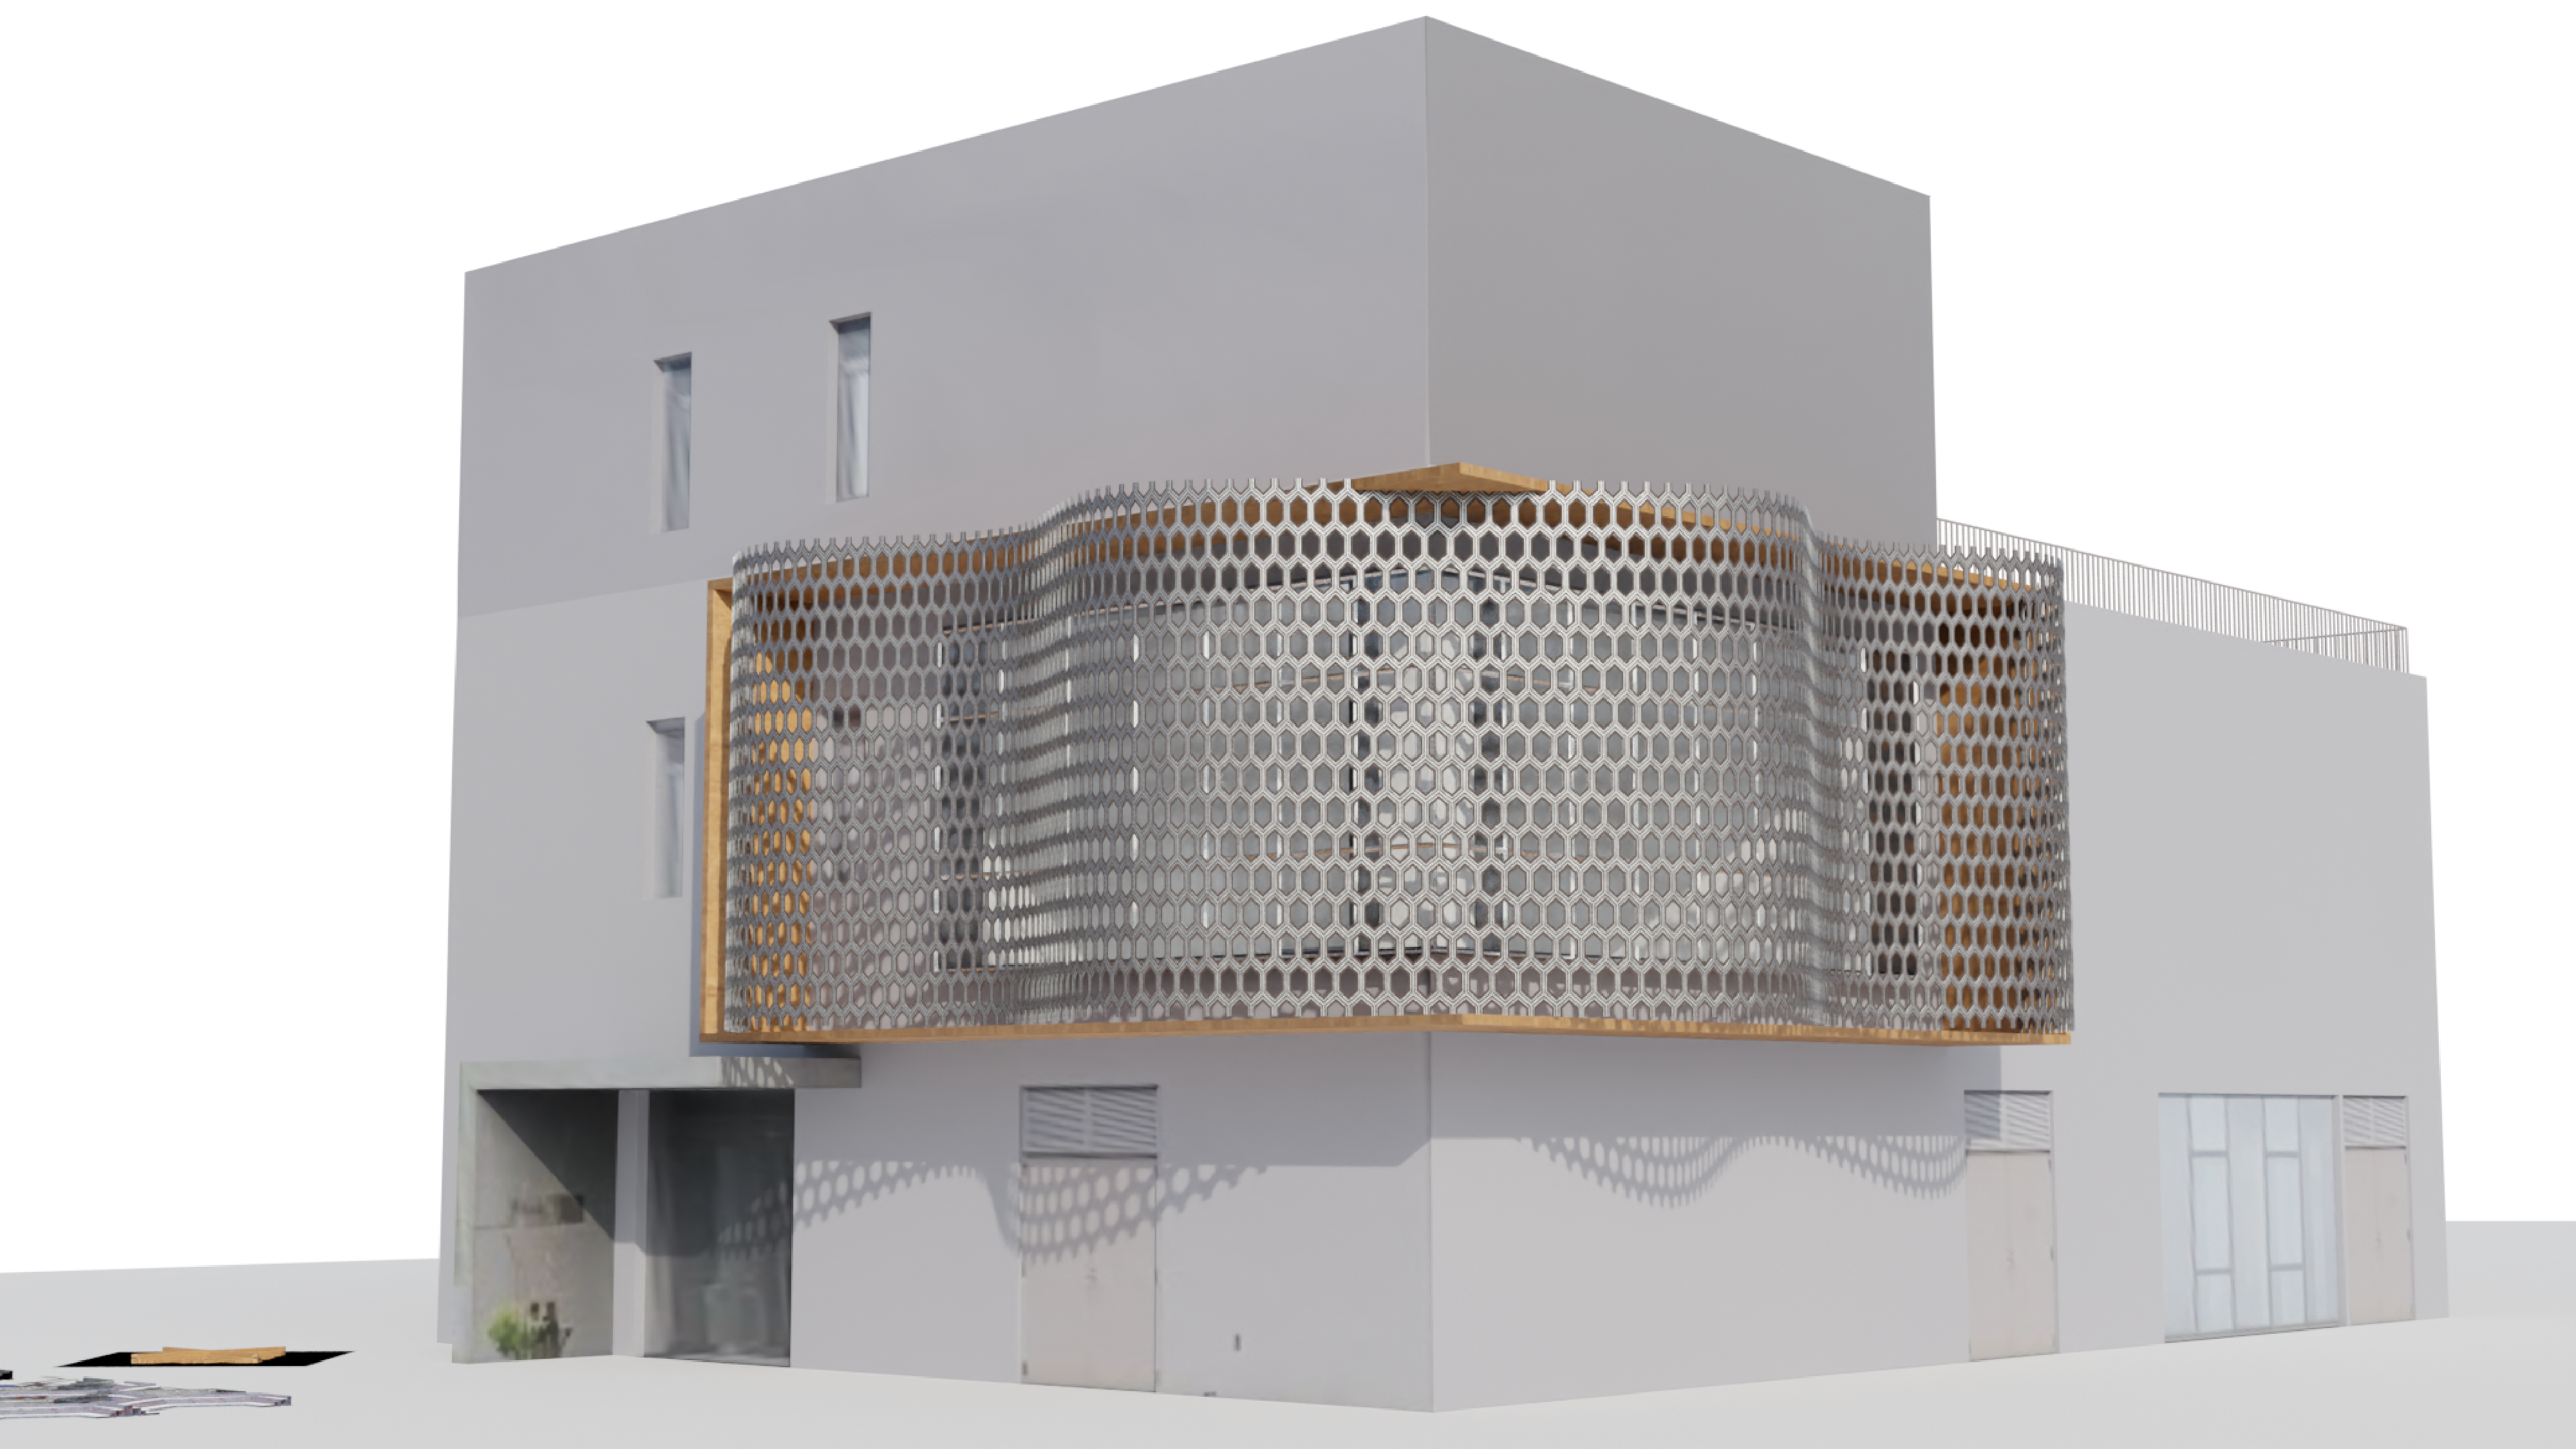
\includegraphics[width=1\linewidth]{Images/Pattern 2/0006}} &
              {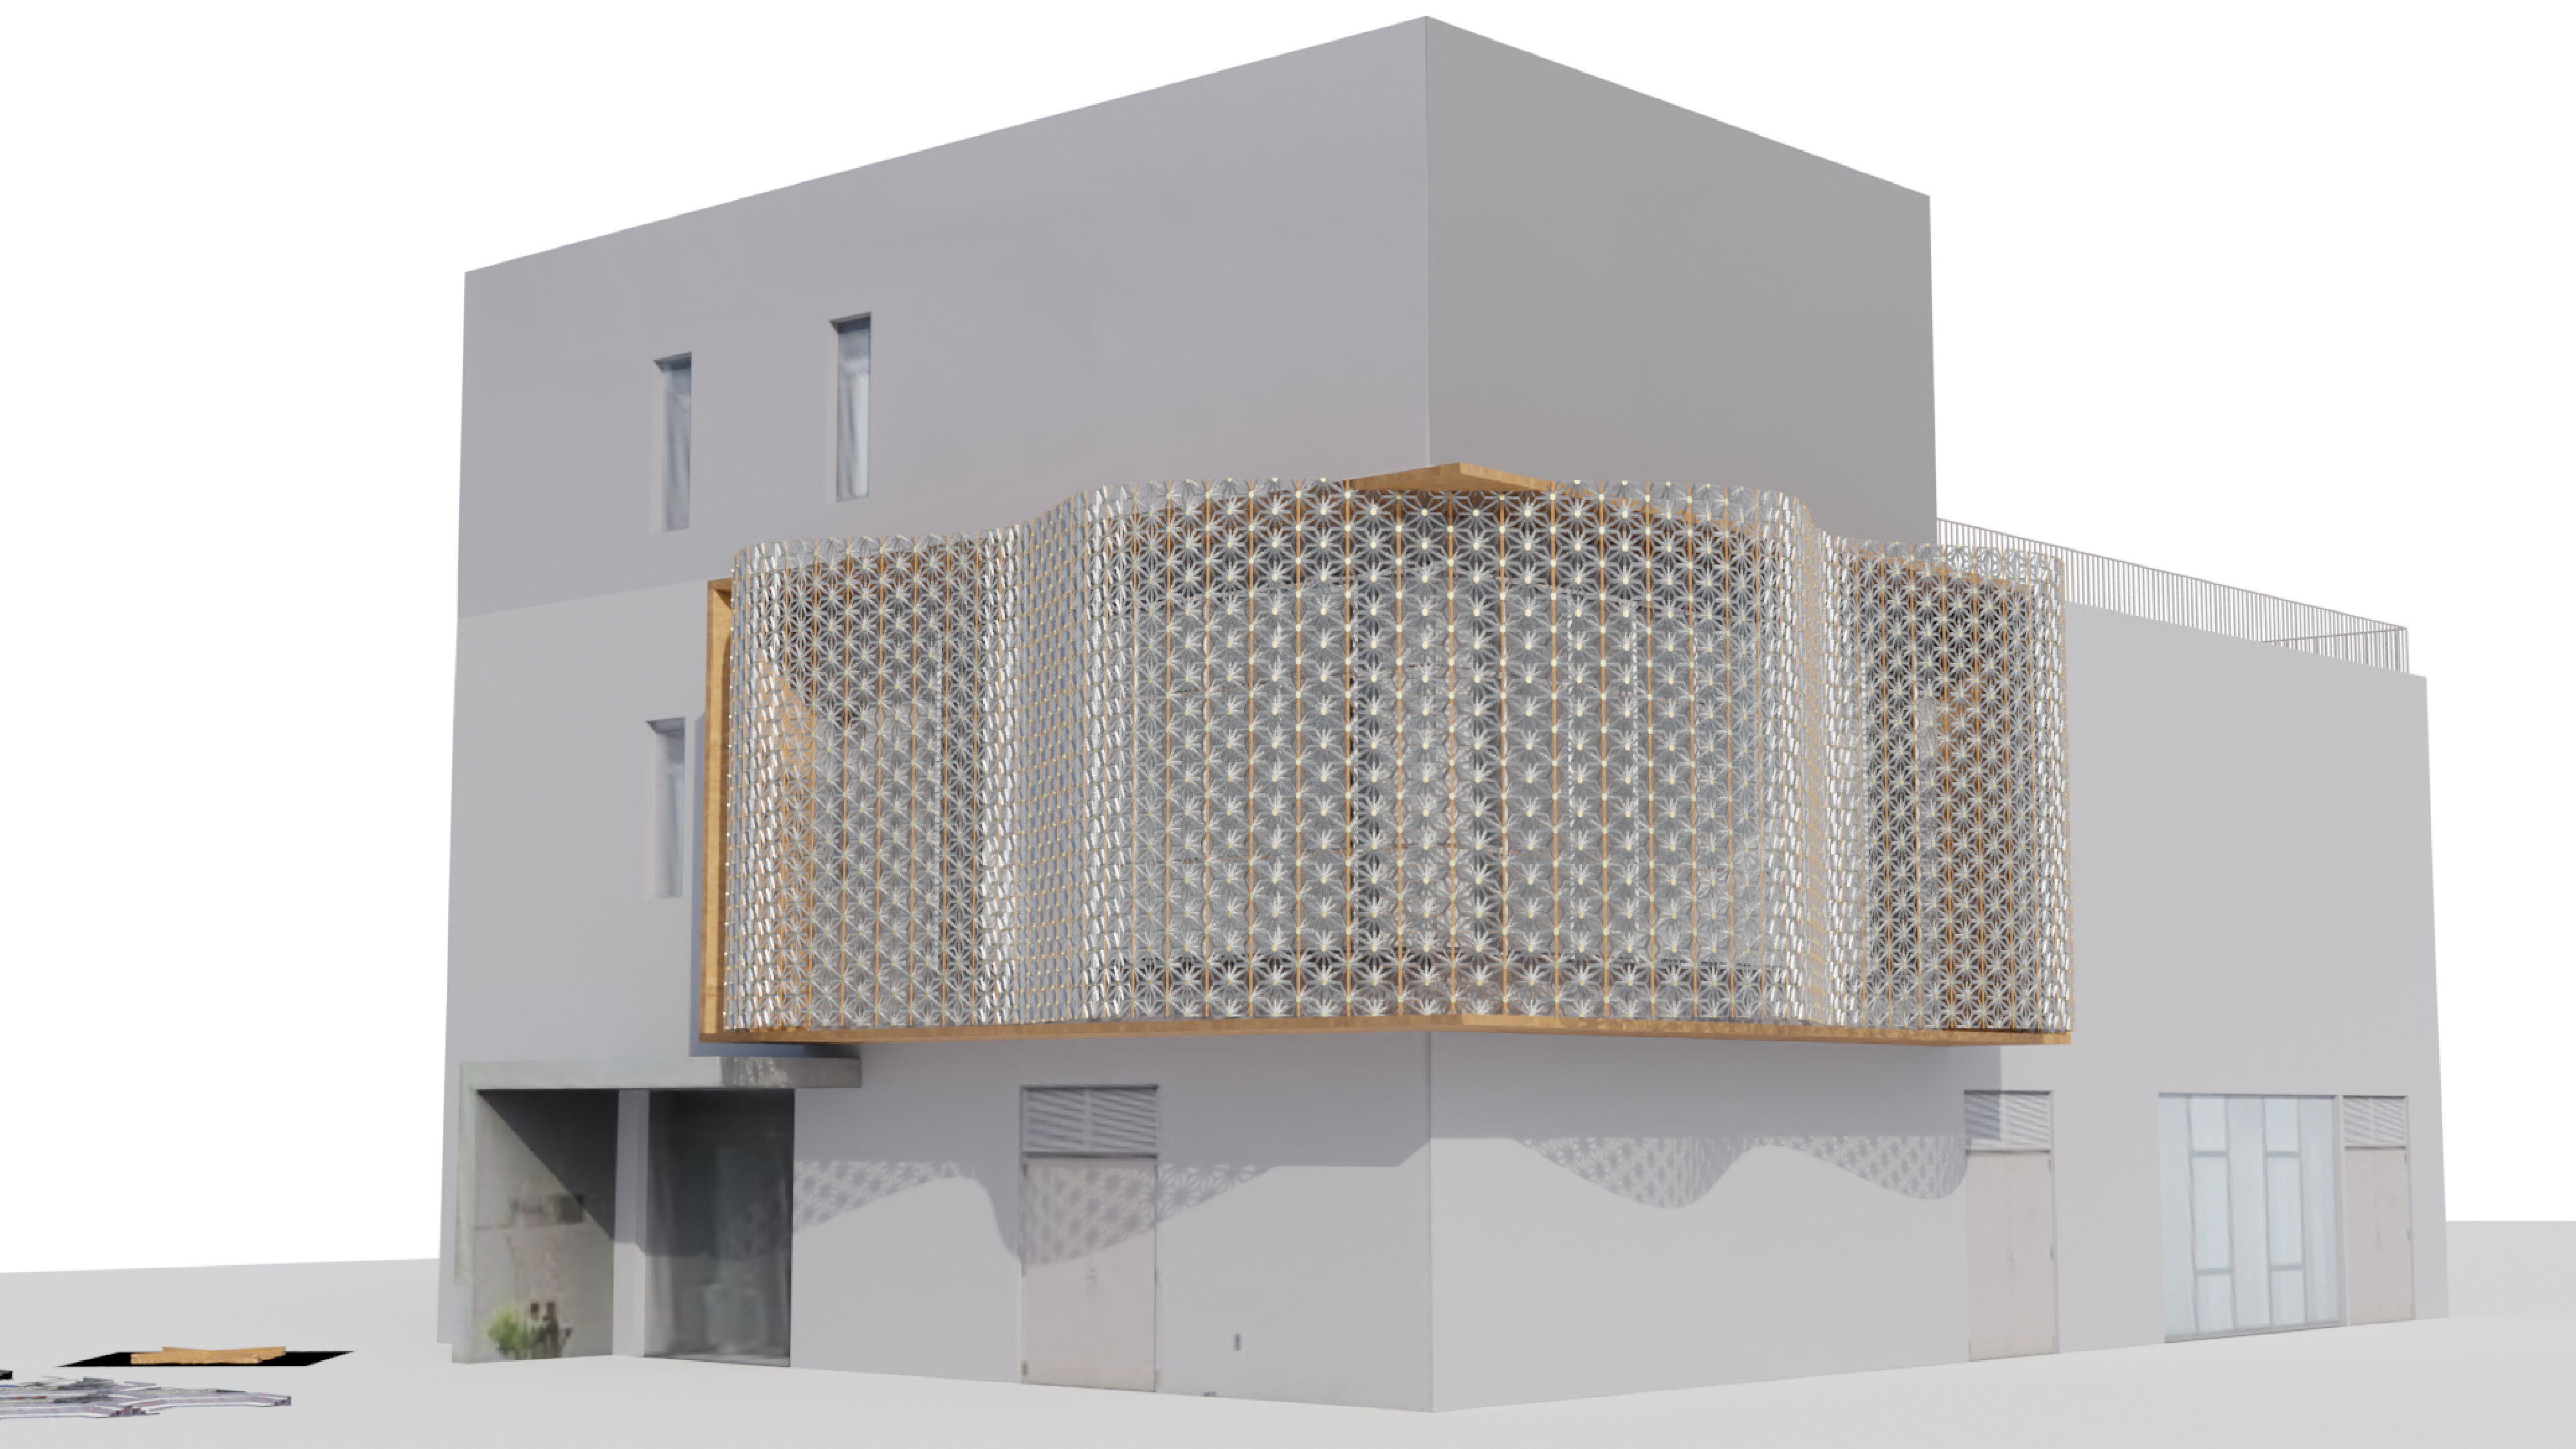
\includegraphics[width=1\linewidth]{Images/Pattern 3/0006}} \\
            \midrule
            \text{Level 9} &  &  &
            \\
            {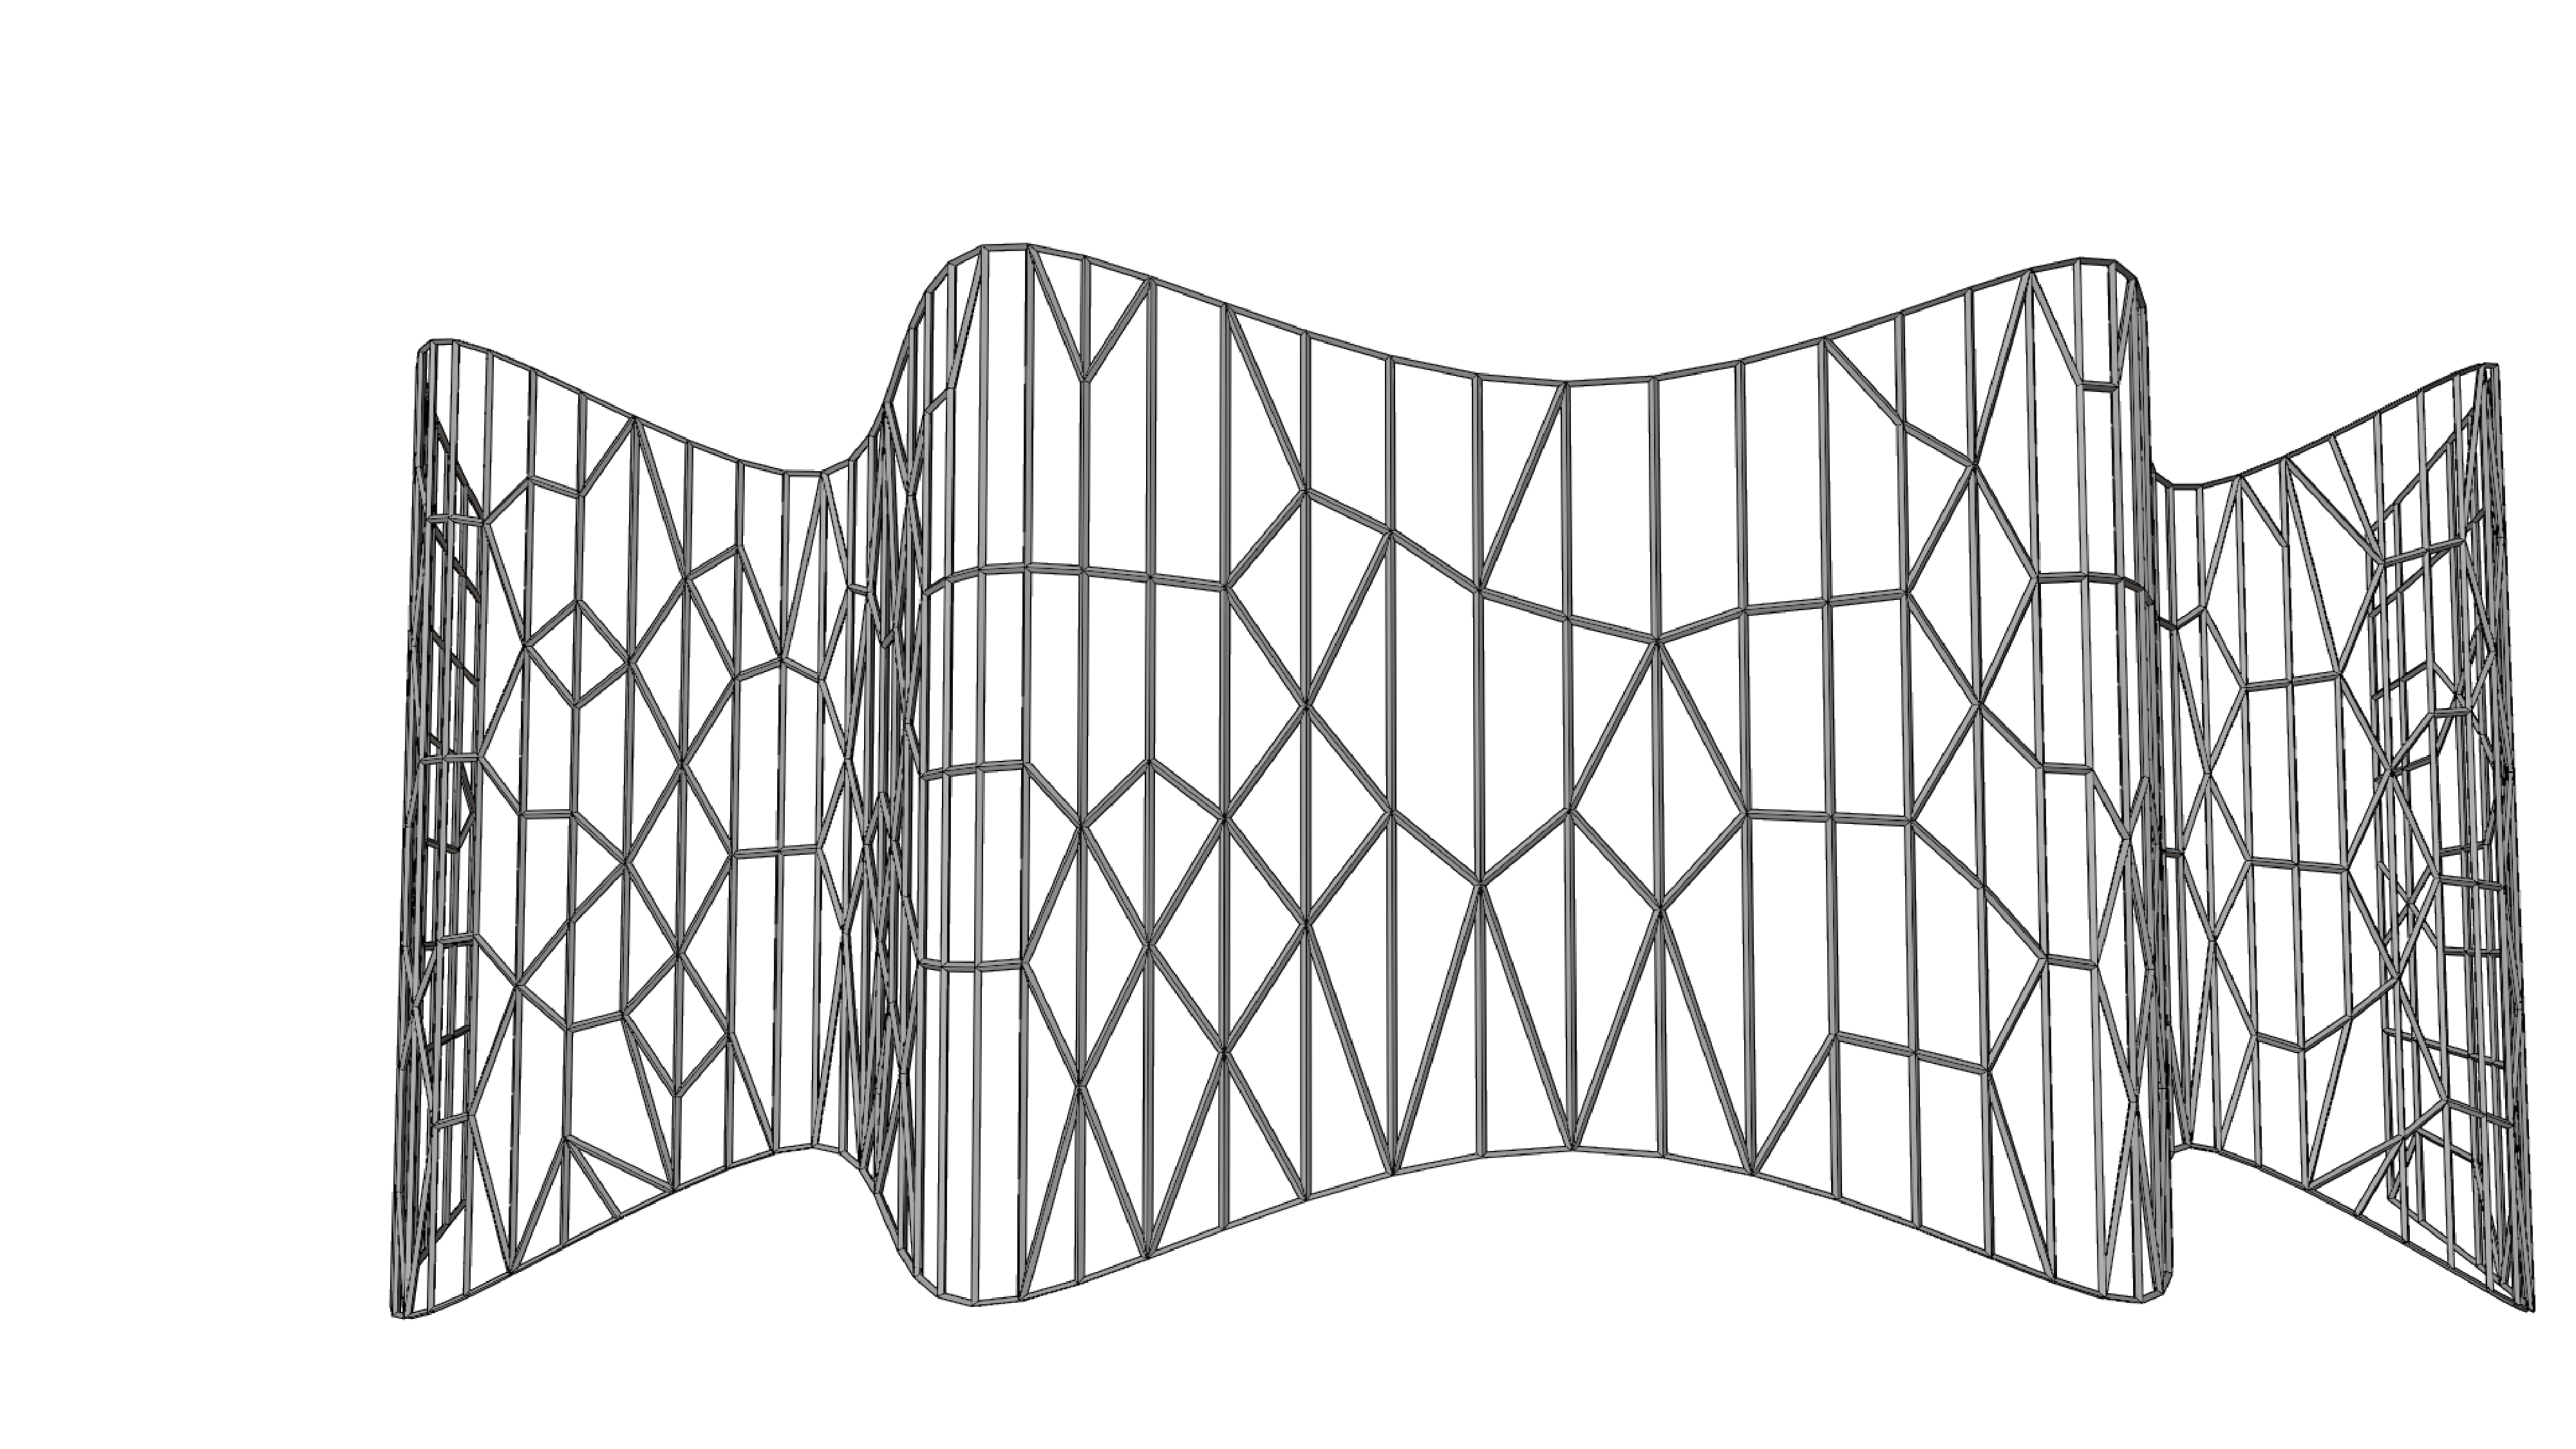
\includegraphics[width=1\linewidth]{Images/Wall 0/0009}} &
              {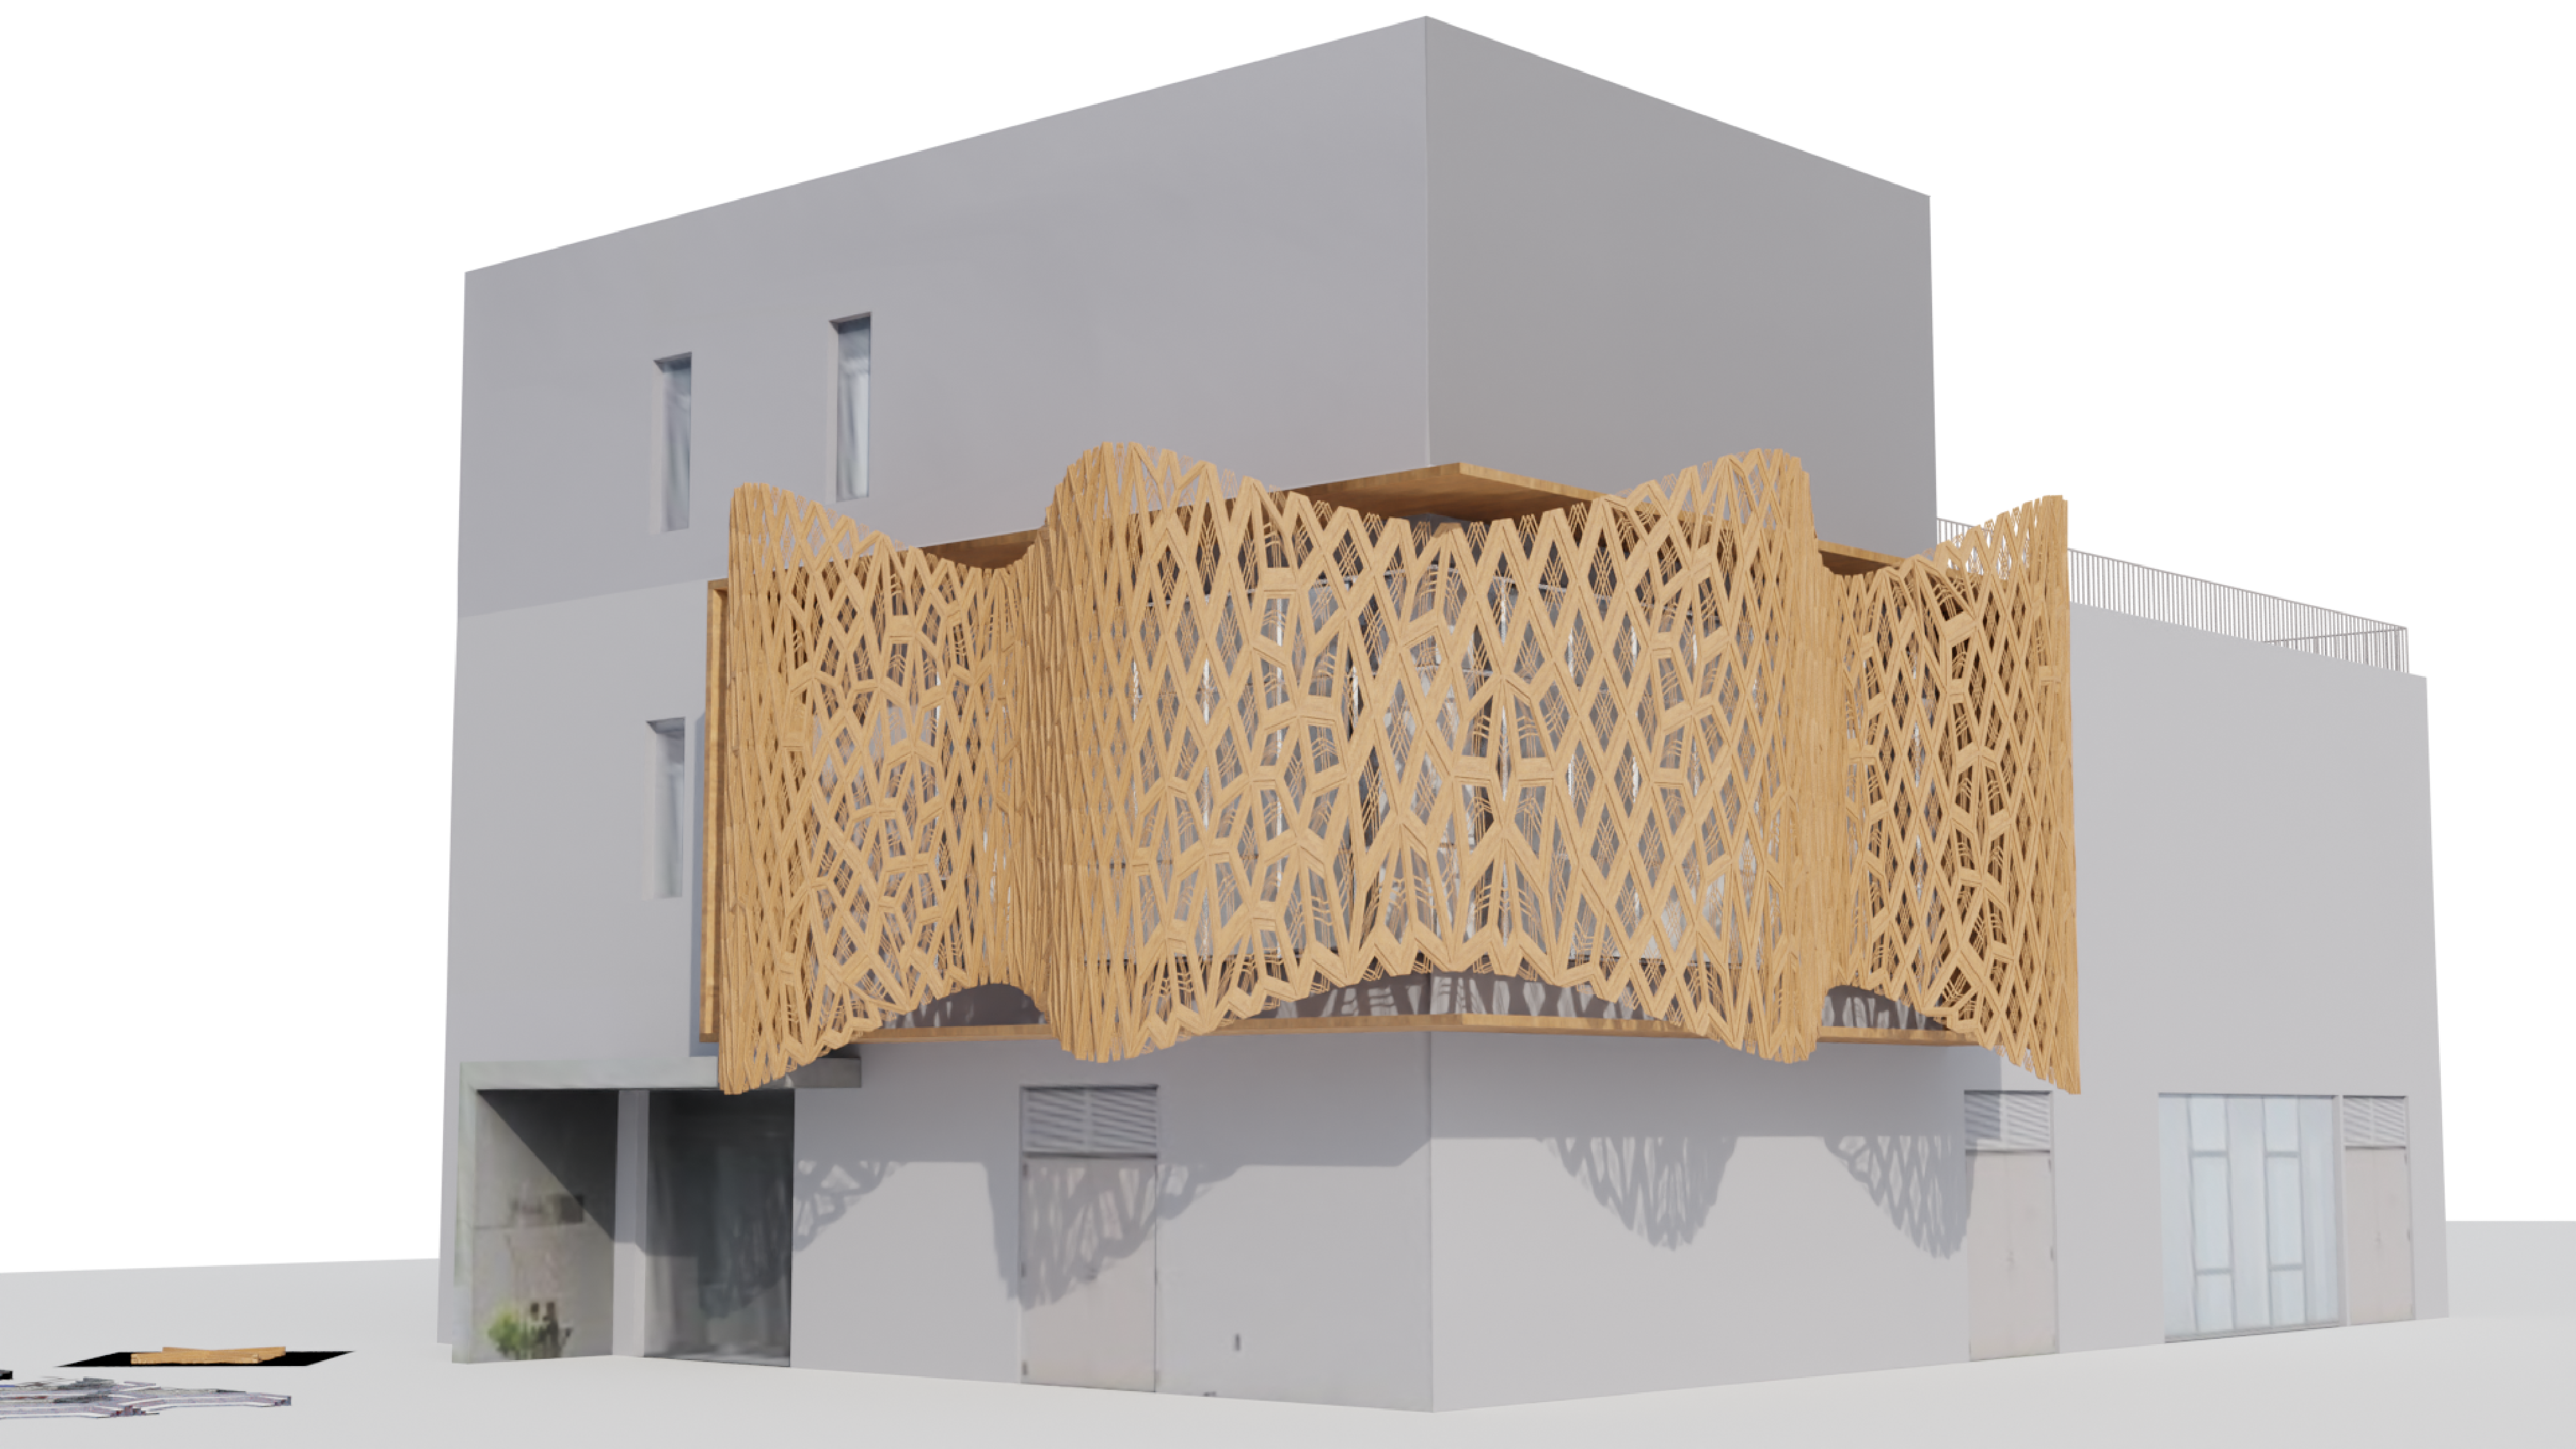
\includegraphics[width=1\linewidth]{Images/Pattern 1/0009}} &
              {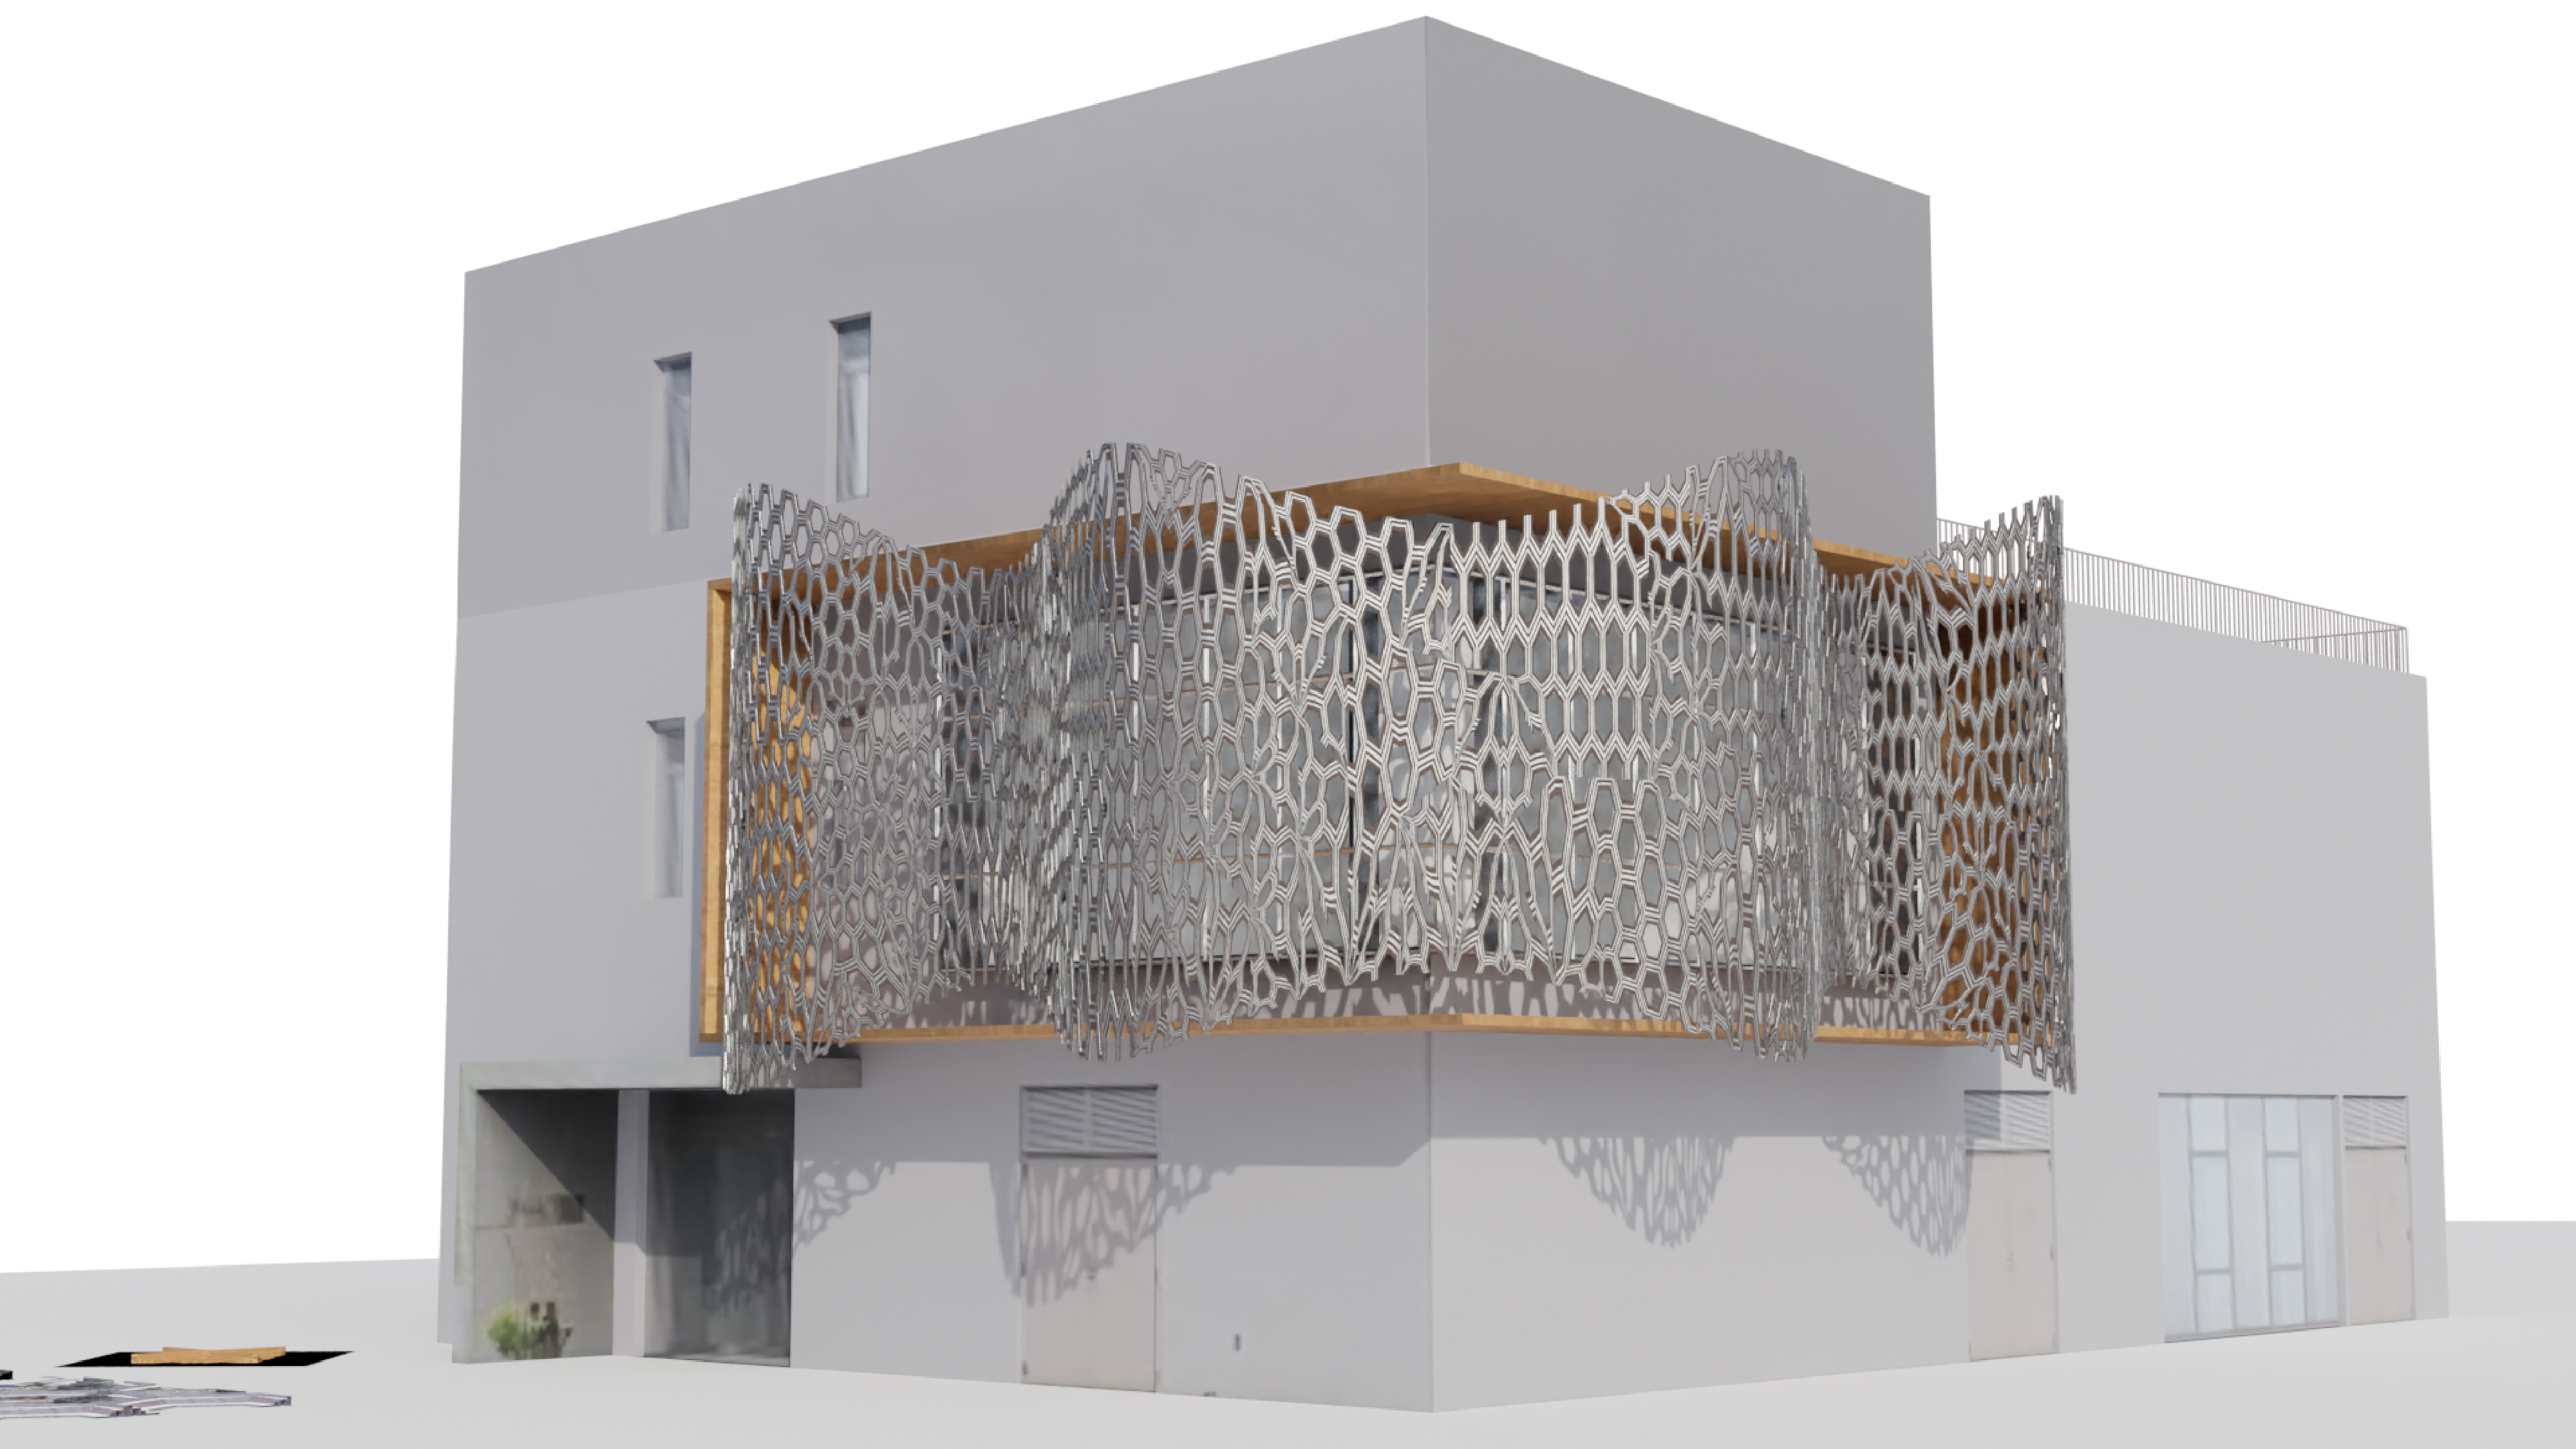
\includegraphics[width=1\linewidth]{Images/Pattern 2/0009}} &
              {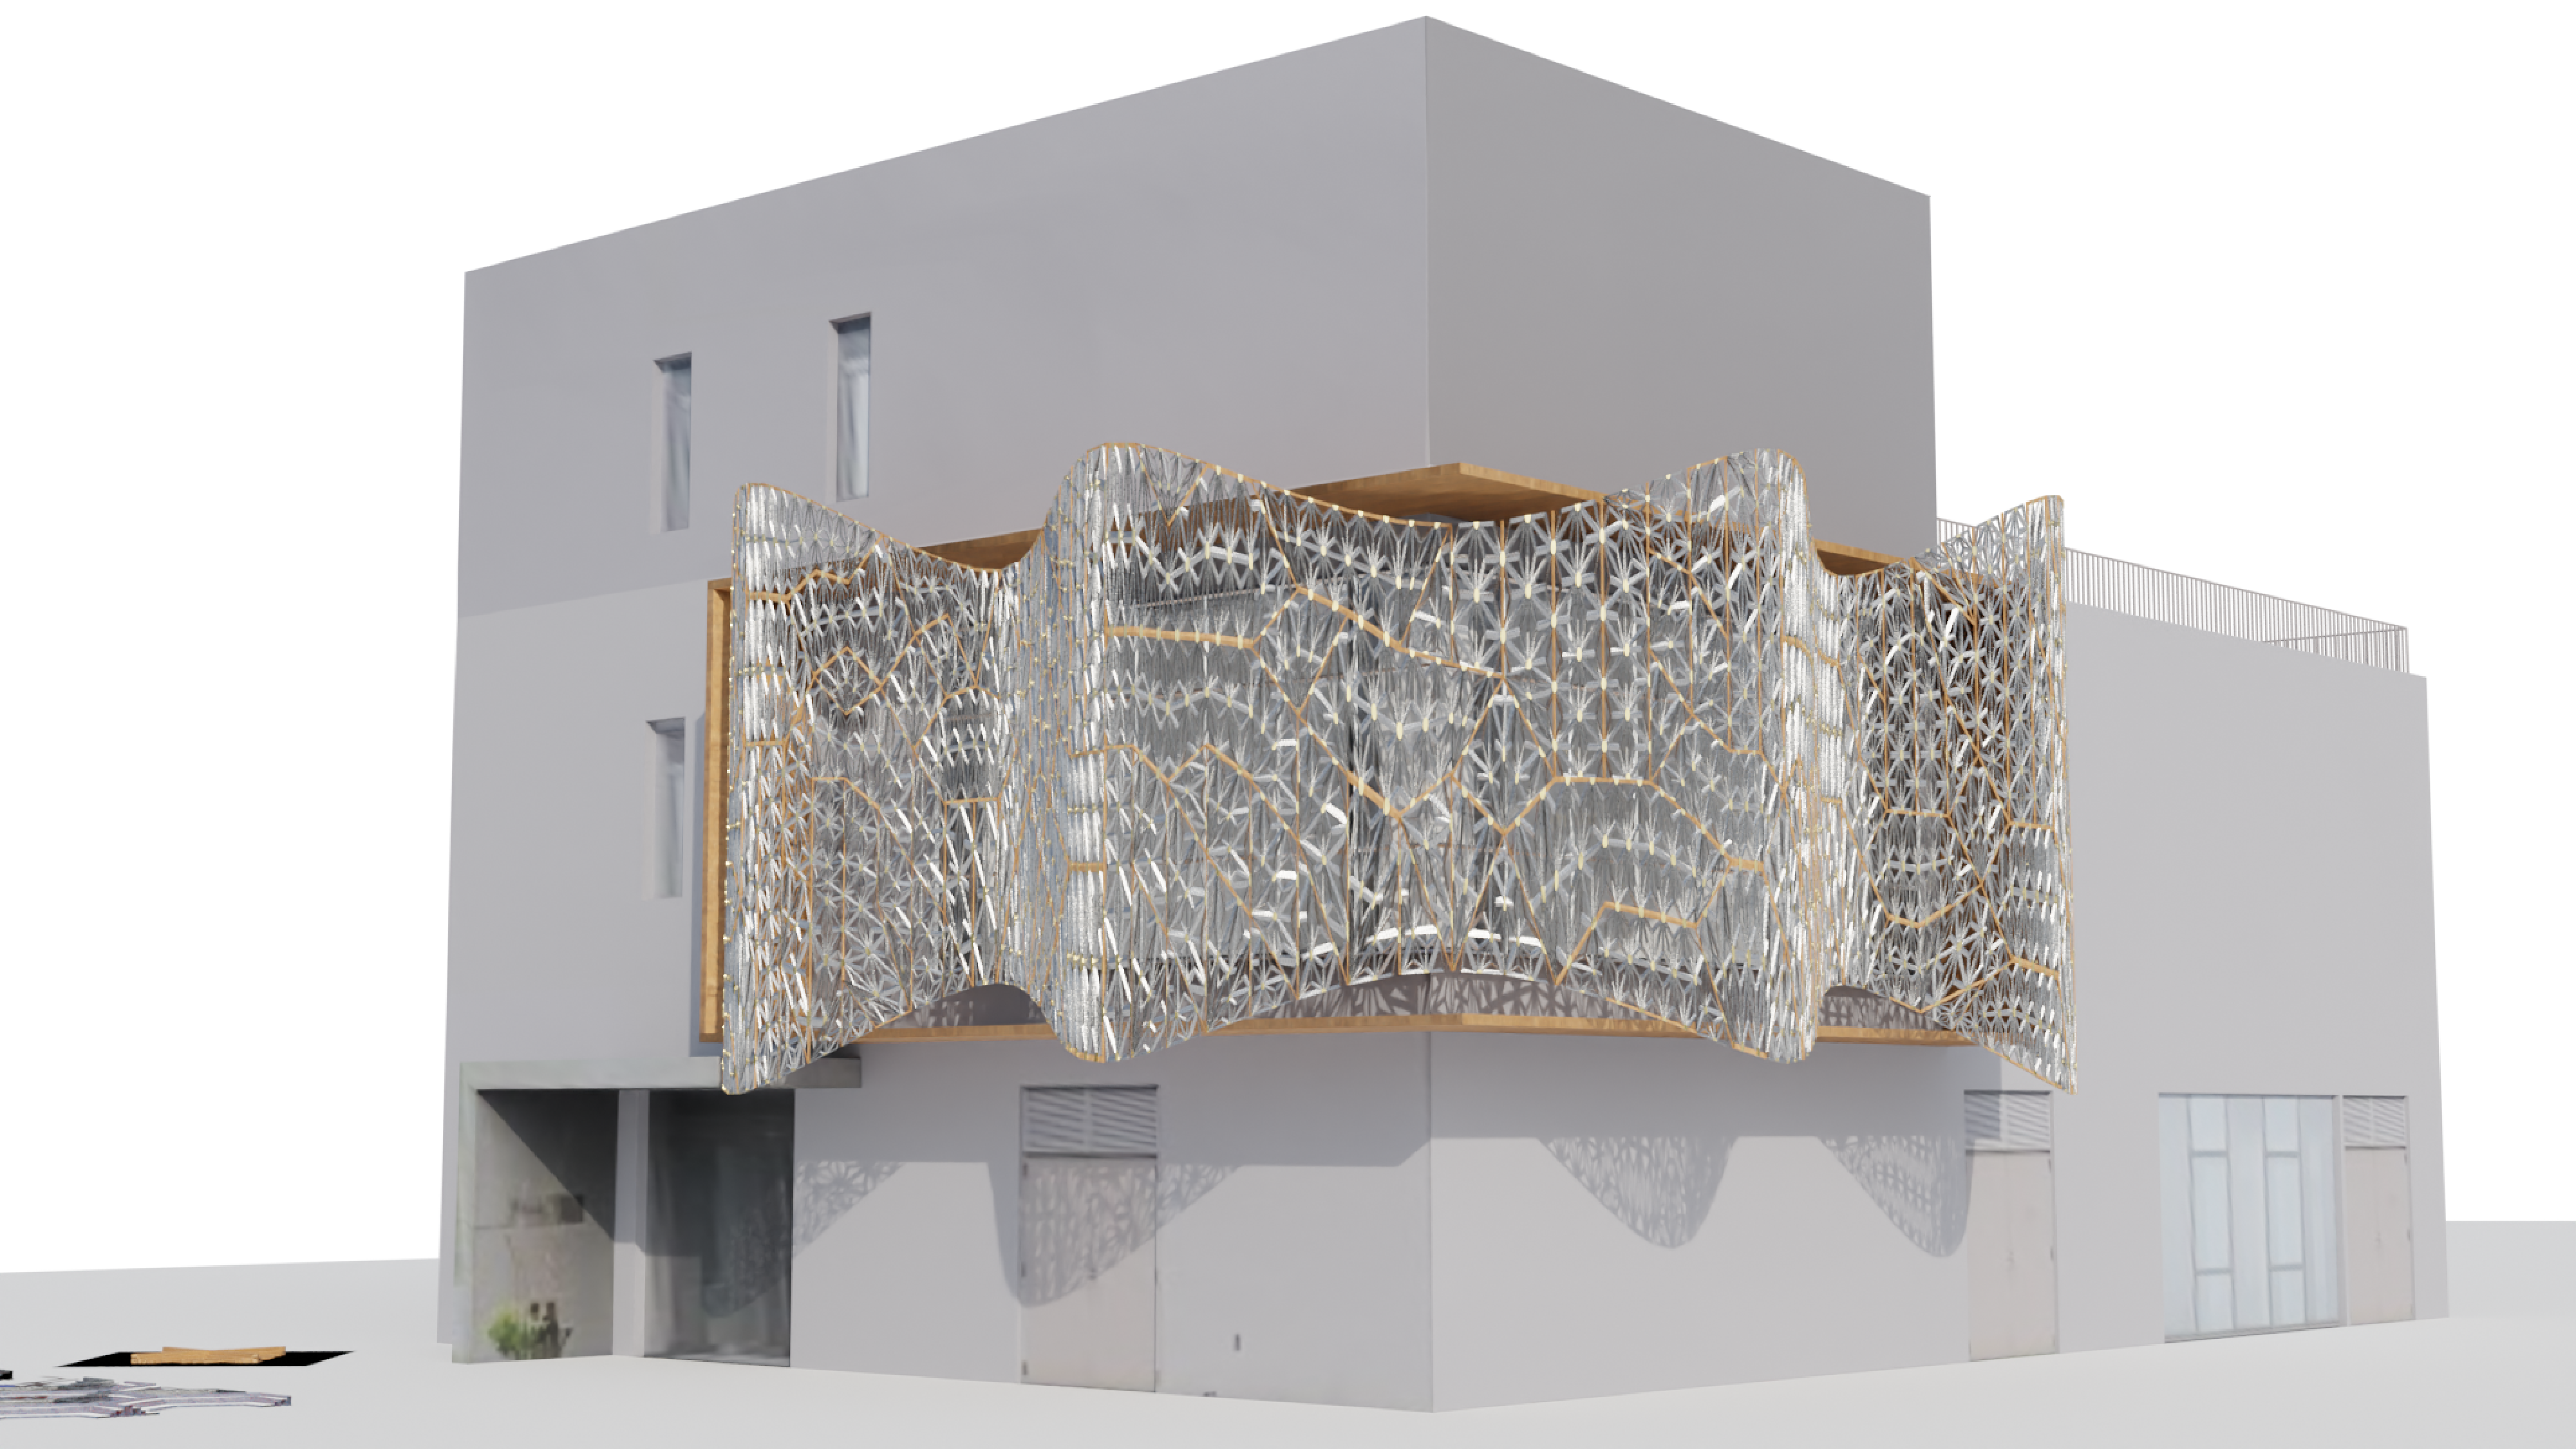
\includegraphics[width=1\linewidth]{Images/Pattern 3/0009}} \\
            \bottomrule
        \end{tabularx}
    \end{table*}


Ensuring a high level of realism is paramount in Virtual Reality simulation, particularly when aiming to replicate a genuine experience.
In the context of this research, our objective is to assess the reactions of individuals within a building adorned with facades of varying complexity.
Therefore, the precision of our 3D modeling is of utmost significance.

For this purpose, the ``3D modeling'' module realized in Blender (v3.6), serves as the first component and is responsible for generating the 3D models central to our research that include the site and building as a virtual environment where the experiment will be conducted and generating the distinctive facade variations.

The virtual environment created is an exact replica of the Architectural Environment Research Building, also known as Building HE20, which houses our laboratory on the Itoshima campus of Kyushu University (see Figure\ref{fig:RealVs3dModel}).

    %% Figure of Real building next to 3D modeled building
     \begin{figure}[t]
          \centering
          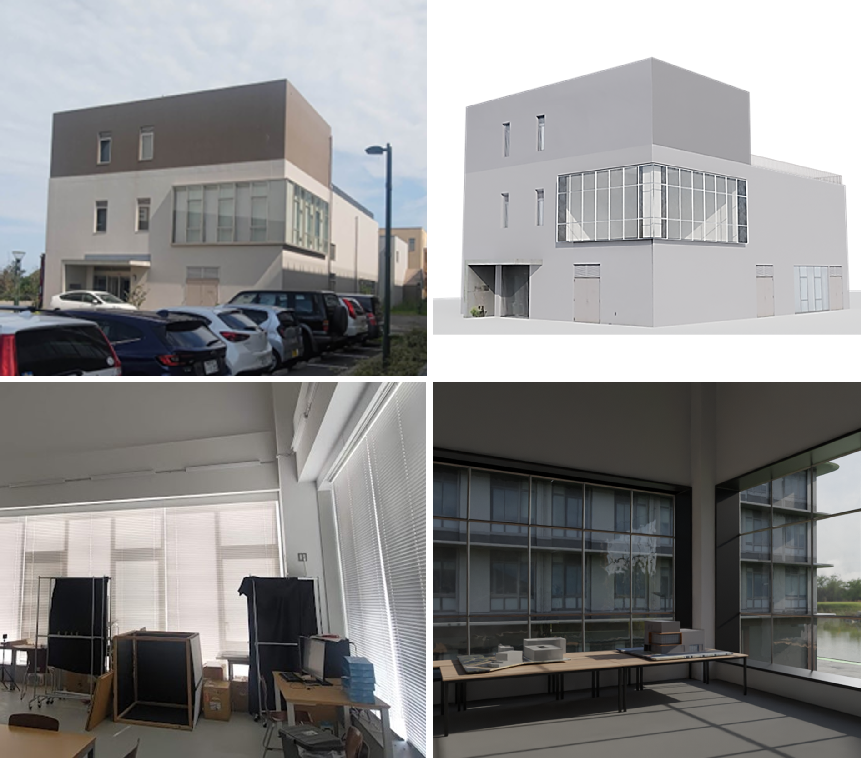
\includegraphics[width= \linewidth]{Images/Realvs3DmodelBlender}
          \caption{Side-by-side comparison of the Architectural Environment Building at Kyushu University used in the experiment, featuring actual interior and exterior photographs (left), and its virtual clone meticulously modeled and rendered in Blender (v3.6) for the Facade Design Complexity Analysis experiment.}
          \label{fig:RealVs3dModel}
        \end{figure}

To ensure an authentic experience, both the exterior of the building and the interior laboratory spaces were meticulously modeled to match the real-world dimensions.
This meticulous approach allows participants to seamlessly navigate the laboratory and revisit their initial encounters with the building's actual conditions, providing a basis for comparison with the virtual simulations.

With the building and its context successfully simulated, the next step was to establish a systematic workflow for creating facade variations with varying degrees of complexity (\ref{tab:PatternsVariationsPart0}).
Our first task was to identify the specific area of the building where the facade variations would be applied.
In Figure\ref{fig:RealVs3dModel}, you can observe that the laboratory's exterior walls feature two sizable windows facing the front and side of the building.
Remarkably, these windows align precisely with our laboratory space, granting an expansive view of a significant portion of the building's facade from inside the lab.

These large glazed surfaces became the central focus for simulating the facade variations.
They offer a unique opportunity for occupants of the laboratory to experience the facade changes firsthand, creating the sensation of being enveloped by the facade variations.
This approach ensures that participants in the experiment perceive a meaningful impact when the facades change from the interior of the lab, a perspective that would typically only be observed from a distance outside the building.

Once the area for applying the facade variations was identified, consisting of the two prominent windows with glazed curtain walls in the lab, the subsequent step was to extrapolate its base mesh and dimensions.
This formed the starting point for delineating the boundaries of the forthcoming building variations.

To enhance the experiment's diversity and variability in modeling facade variations, we chose to commence with three fundamental base patterns, as illustrated in Table\ref{tab:PatternsVariationsPart0} under the `Base Module' row.
These patterns drew inspiration from traditional Japanese motifs and served as the building blocks for creating ten distinct variations within each pattern, ensuring a comprehensive exploration of facade complexity in our study.

The generation of the ten facade variations involves a systematic process that incrementally accumulates complexity.
This progression from level 1 to level 10 is depicted in Table \ref{tab:PatternsVariationsPart0} under the 'Mesh per complexity level' column and is outlined as follows:

Levels 1 to 3: The base mesh is subdivided, creating smaller modules and increasing the pattern density on the facades.

Level 4: The subdivided mesh from level 3 undergoes a one-axis rotation, resulting in a tilted facade.

Level 5: The tilted facade is further bent along its central horizontal axis, forming a concave mesh.

Level 6: Curvature is applied alternately along the vertical axis, producing a wavy mesh.

Level 7: The previously waved mesh is vertically stretched at alternating points, resulting in variations in module size and spacing.

From Level 8 to Level 10: A decimation process is applied to the uniform mesh.
This process disrupts the uniformity of the mesh with minimal overall shape changes\cite{Blender2023}, achieved by collapsing edges.
This reduces the module count while increasing the randomness of the shape and orientation of the base pattern module, creating more complex and varied pattern configurations.

The decimation process is tuned with a \(20\%\) decimation rate for Level 8, \(40\%\) for level 9 and \(60\%\) for level 10.

Finally, the `3d modeling' component' is capable of generating renderings of each facade variation iteration for all three patterns chosen in this research to serve as input for the `Computational Image Complexity Analysis' (CICA) system.
These renderings serve a crucial role in verifying the complexity levels and establishing the ranking of complexity that will guide participants during the experiment.
By visually representing the facade variations, we ensure that the CICA system has the necessary data to evaluate and score the complexity of each iteration accurately.

With a comprehensive understanding of how the 3D modeling component supports the VR system, let's now delve into the application of the CICA system for ranking the 3D-modeled facades.
This process is integral to our Virtual Reality (VR) experiment, where participants will engage with facades featuring various complexity levels.



%
%To represent common challenges in site layout design, we selected three simulated sites (Table \ref{tab:SiteParametersAndPreview}), which included variations in slopes, gradients, and the need to preserve natural features. While these sites were fictitious, they were modeled based on the geographical properties of Fukuoka, Japan, where the experiment was conducted.
%
%The building in the simulation was designed to be photo-realistic (Figure \ref{fig:BuidlingSiteBlenderSimulation}) and served as a focal point for users to explore different positions on the terrain. The "optimization algorithm" of this system (see Figure \ref{fig:MOO_Flowchart}) extracted the building's dimensions, particularly its boundaries, to use them as input to define the building footprint and calculate its impact on the site during the Site Layout Planning process (Table \ref{tab:BuildingParameters}).

    %%Table: Pattern Variations sample 3, 6, 9
    \begin{table*}[htb]
        \centering
        \small
        \caption{Patterns variations for the First five levels of complexity}
        \label{tab:PatternsVariationsPart0}
        \begin{tabularx}
        {\textwidth}{p{4cm} >{\centering\arraybackslash}X >{\centering\arraybackslash}X >{\centering\arraybackslash}X }
            \toprule
            \textit{Description} &
              \textit{Pattern 1} &
              \textit{Pattern 2} &
              \textit{Pattern 3} \\
            \midrule
            \text{Pattern Name} & Hishi Pattern & Tortoise shells & Asanoha Pattern\\

            \midrule
            \textit{Base Module} &  &  &
            \\
            {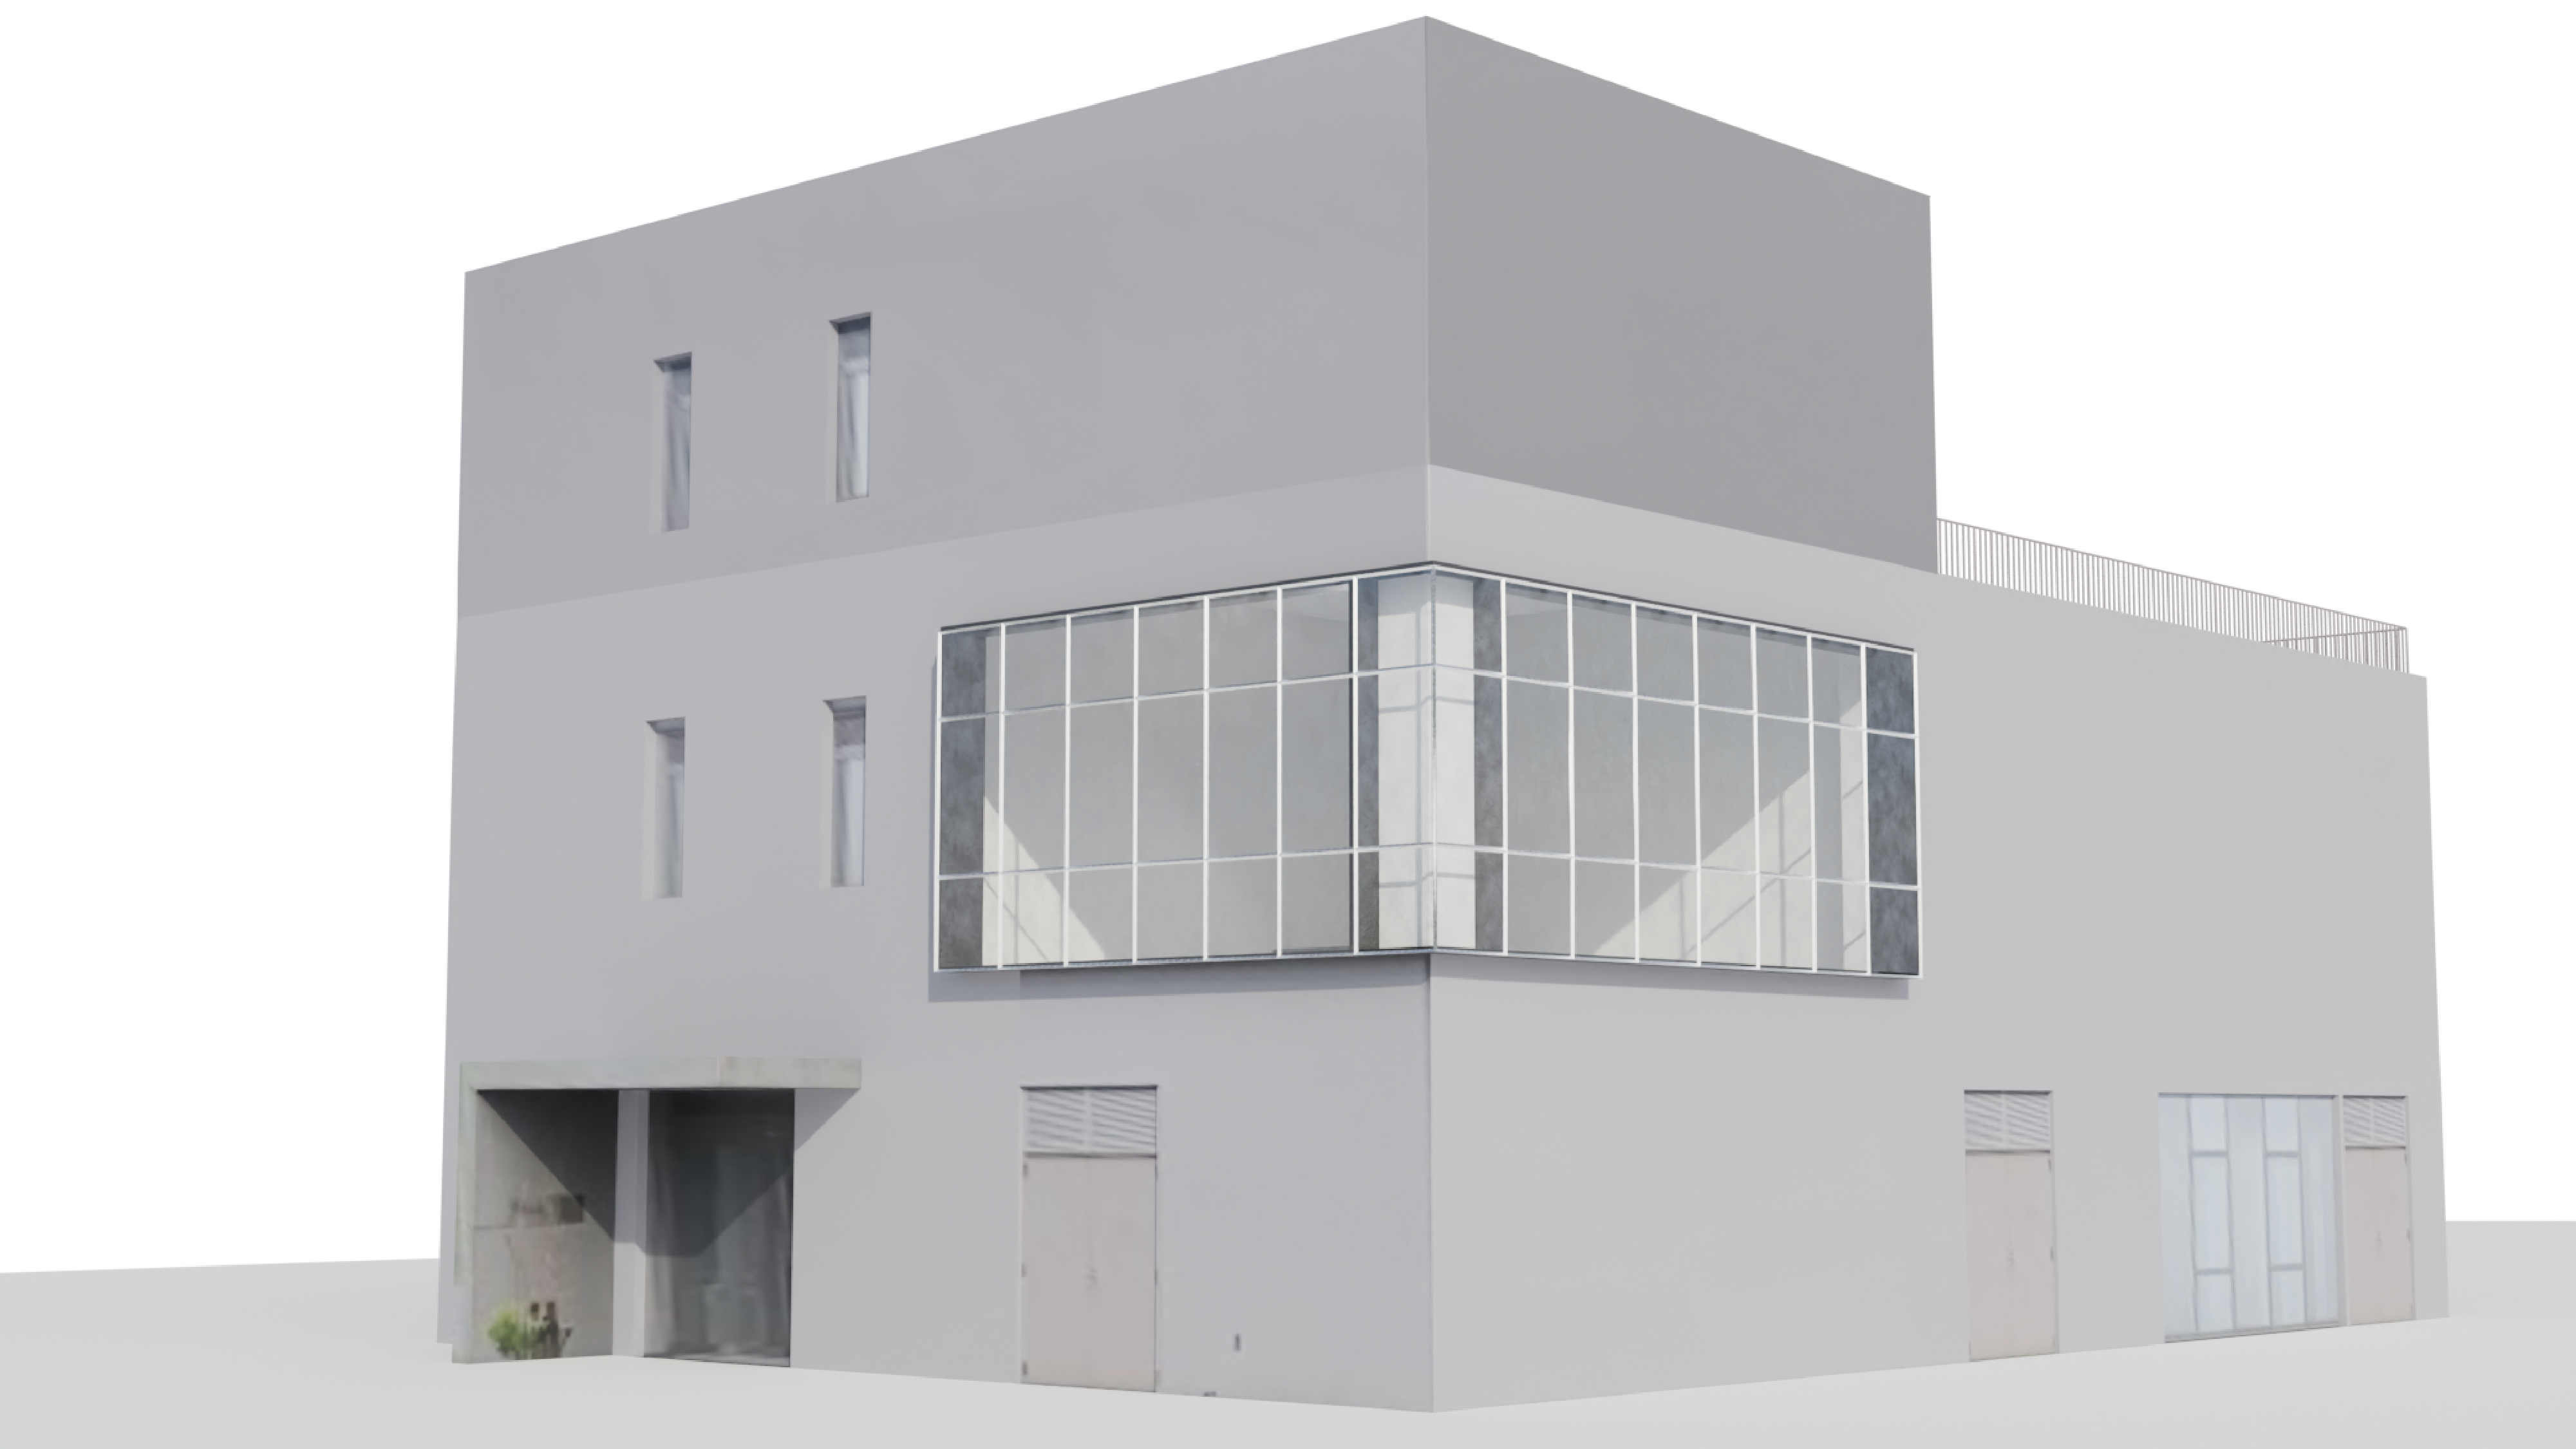
\includegraphics[width=1\linewidth]{Images/Base Module/Building}} &
              {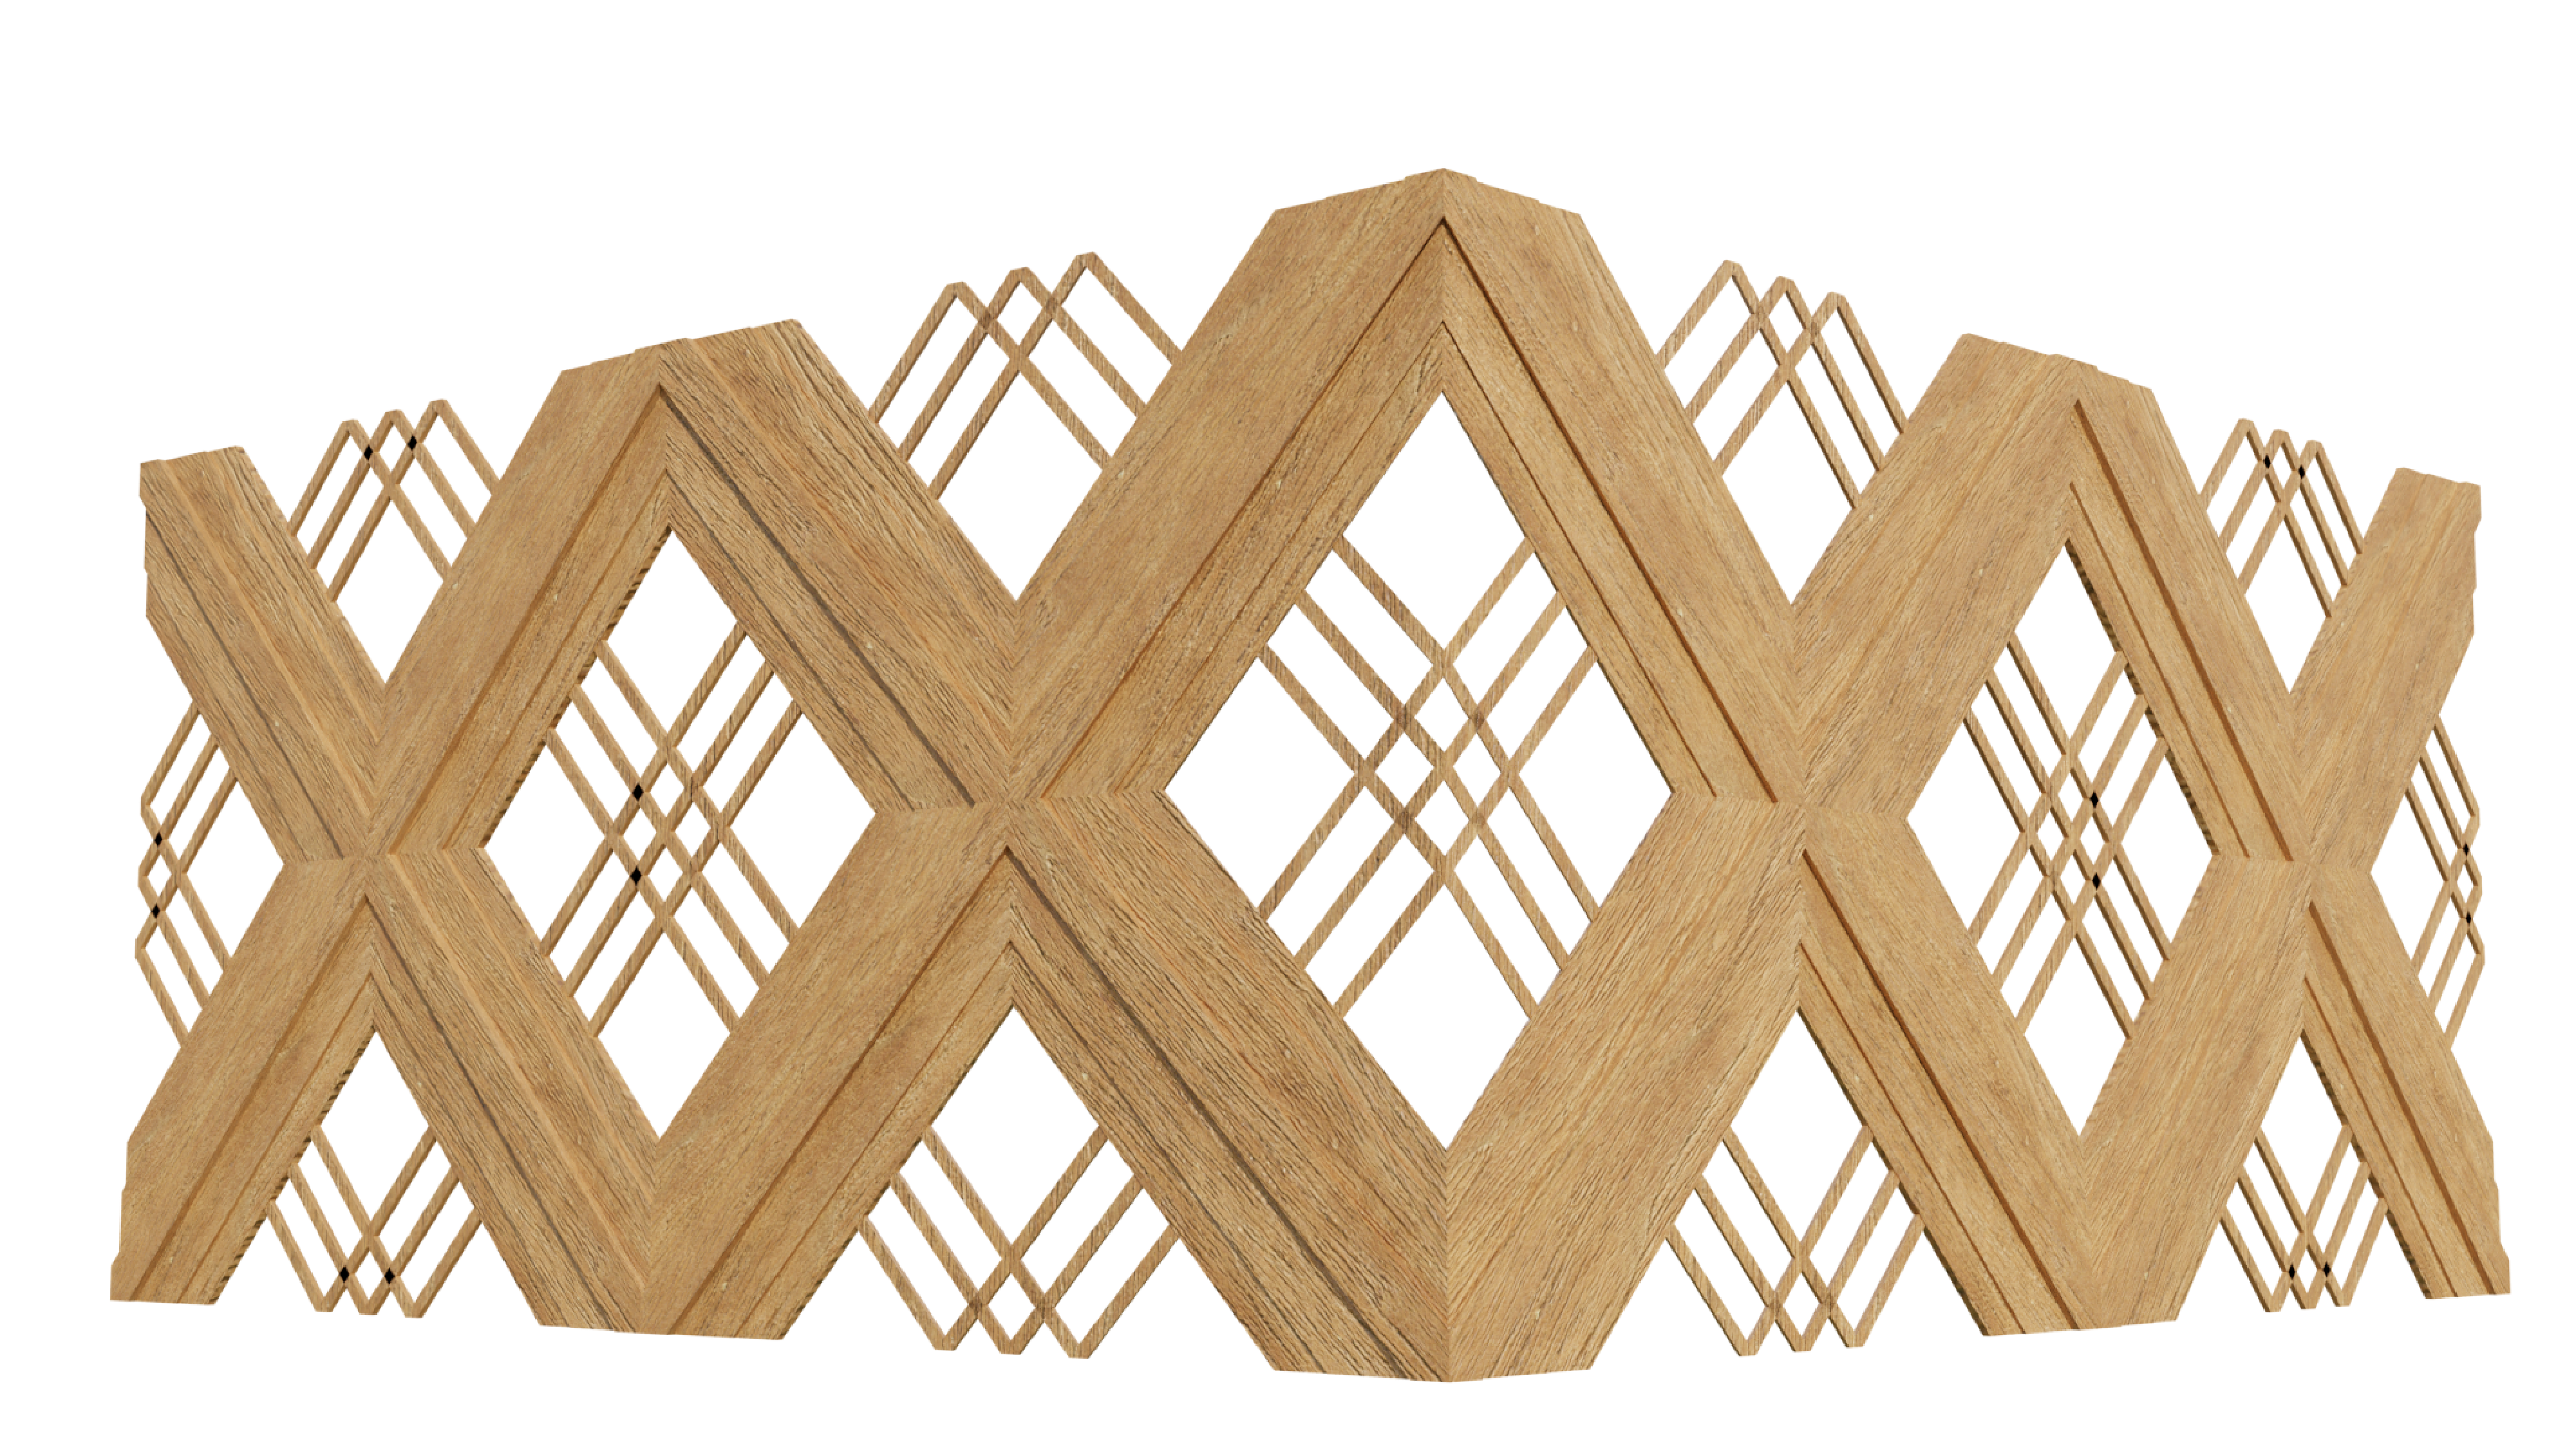
\includegraphics[width=1\linewidth]{Images/Base Module/Pattern1}} &
              {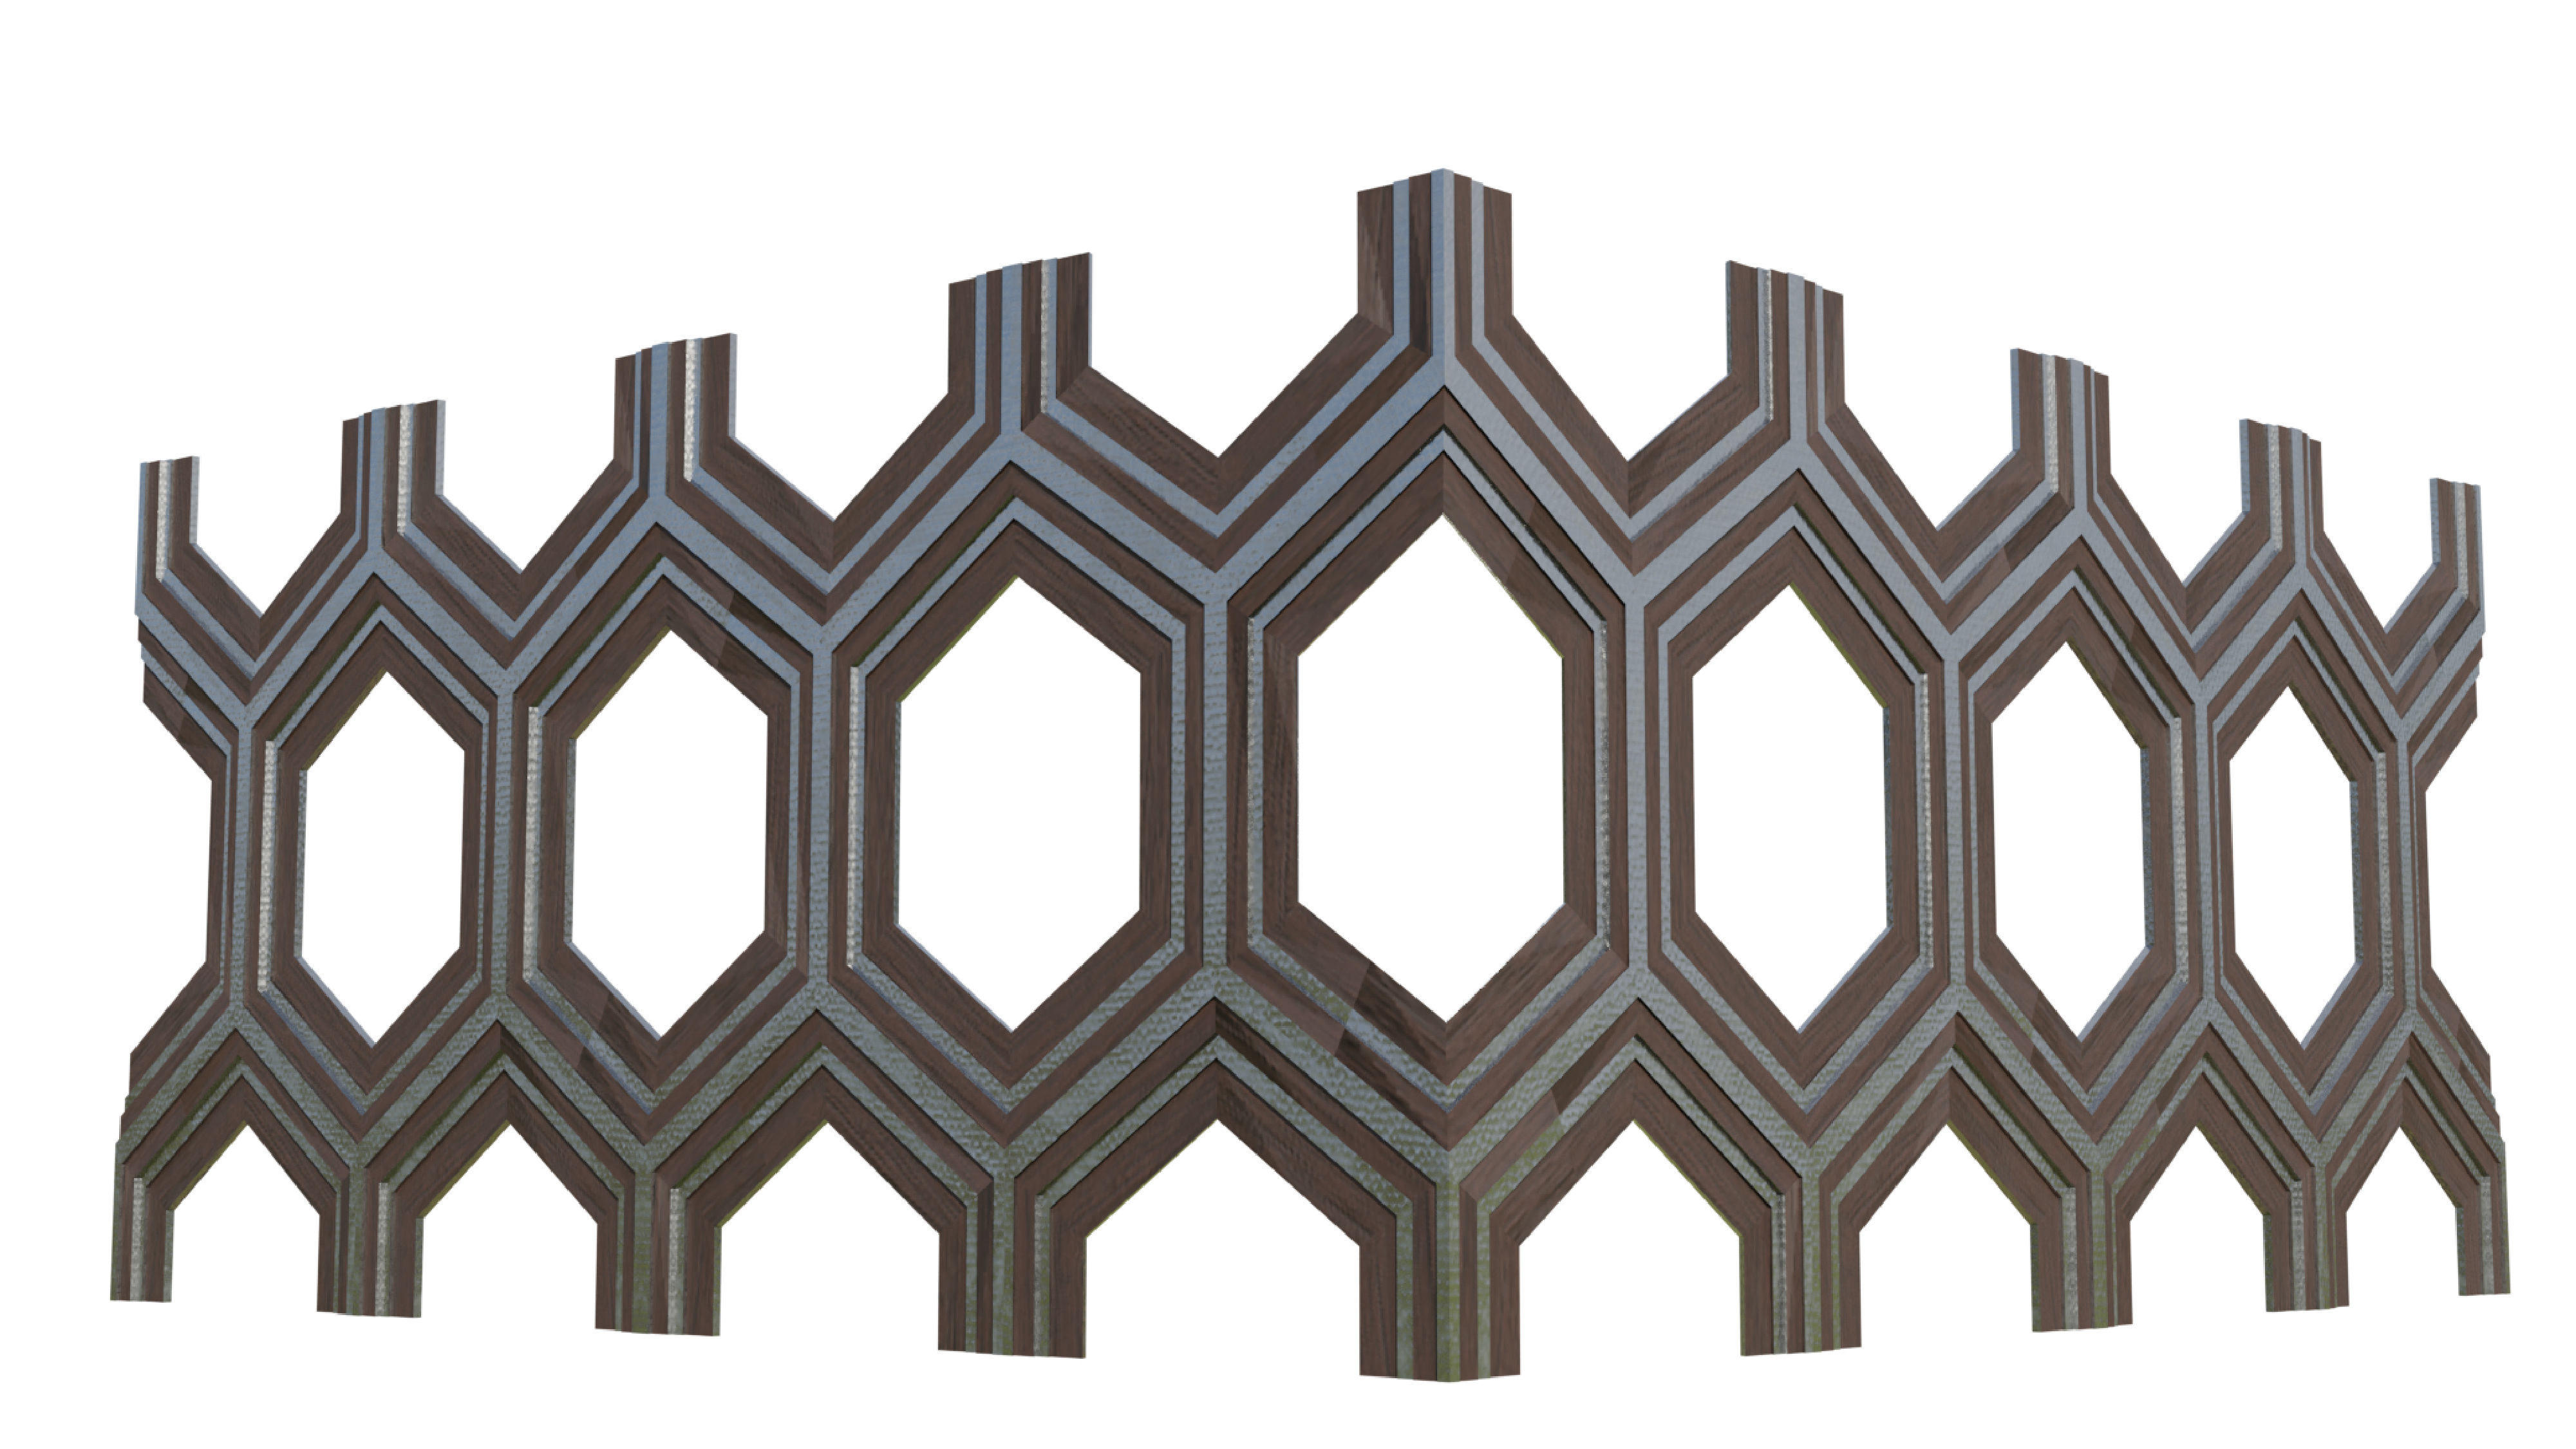
\includegraphics[width=1\linewidth]{Images/Base Module/Pattern2}} &
              {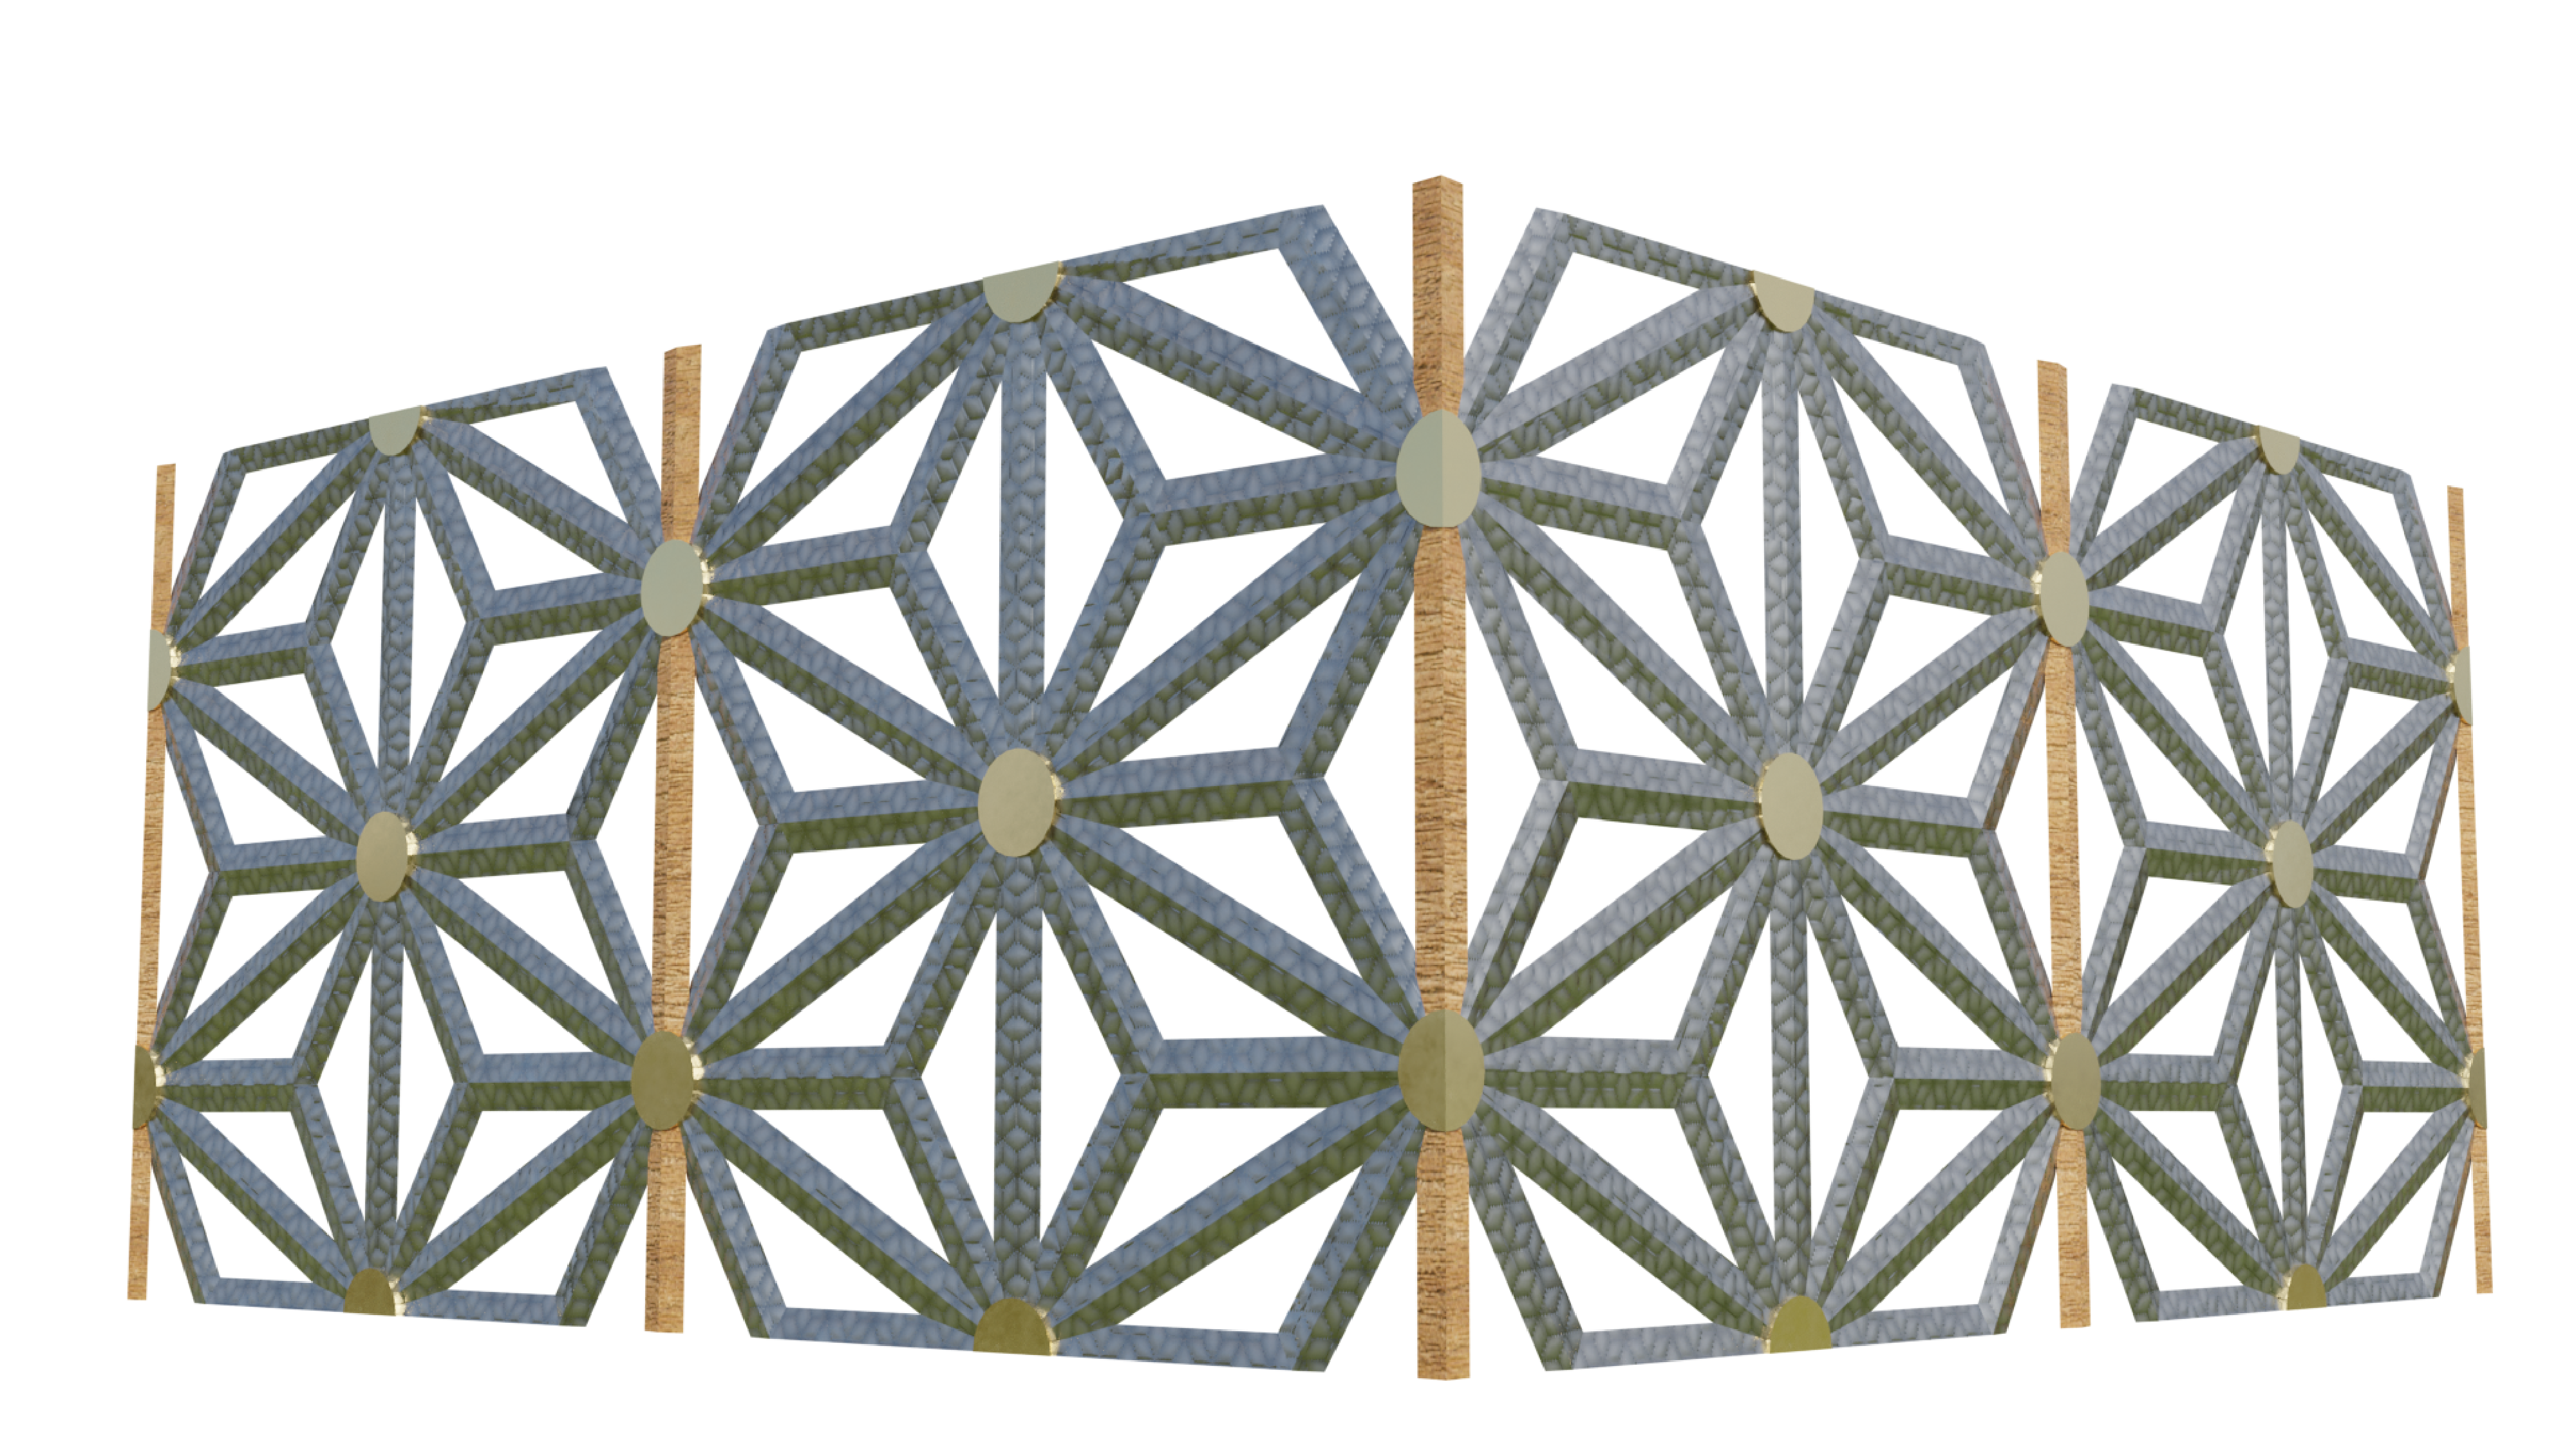
\includegraphics[width=1\linewidth]{Images/Base Module/Pattern3}} \\

            \midrule
            \textit{Mesh per complexity Level} &
              \textit{Pattern 1} &
              \textit{Pattern 2} &
              \textit{Pattern 3}\\

            \midrule
            \text{Level 3} &  &  &
            \\
            {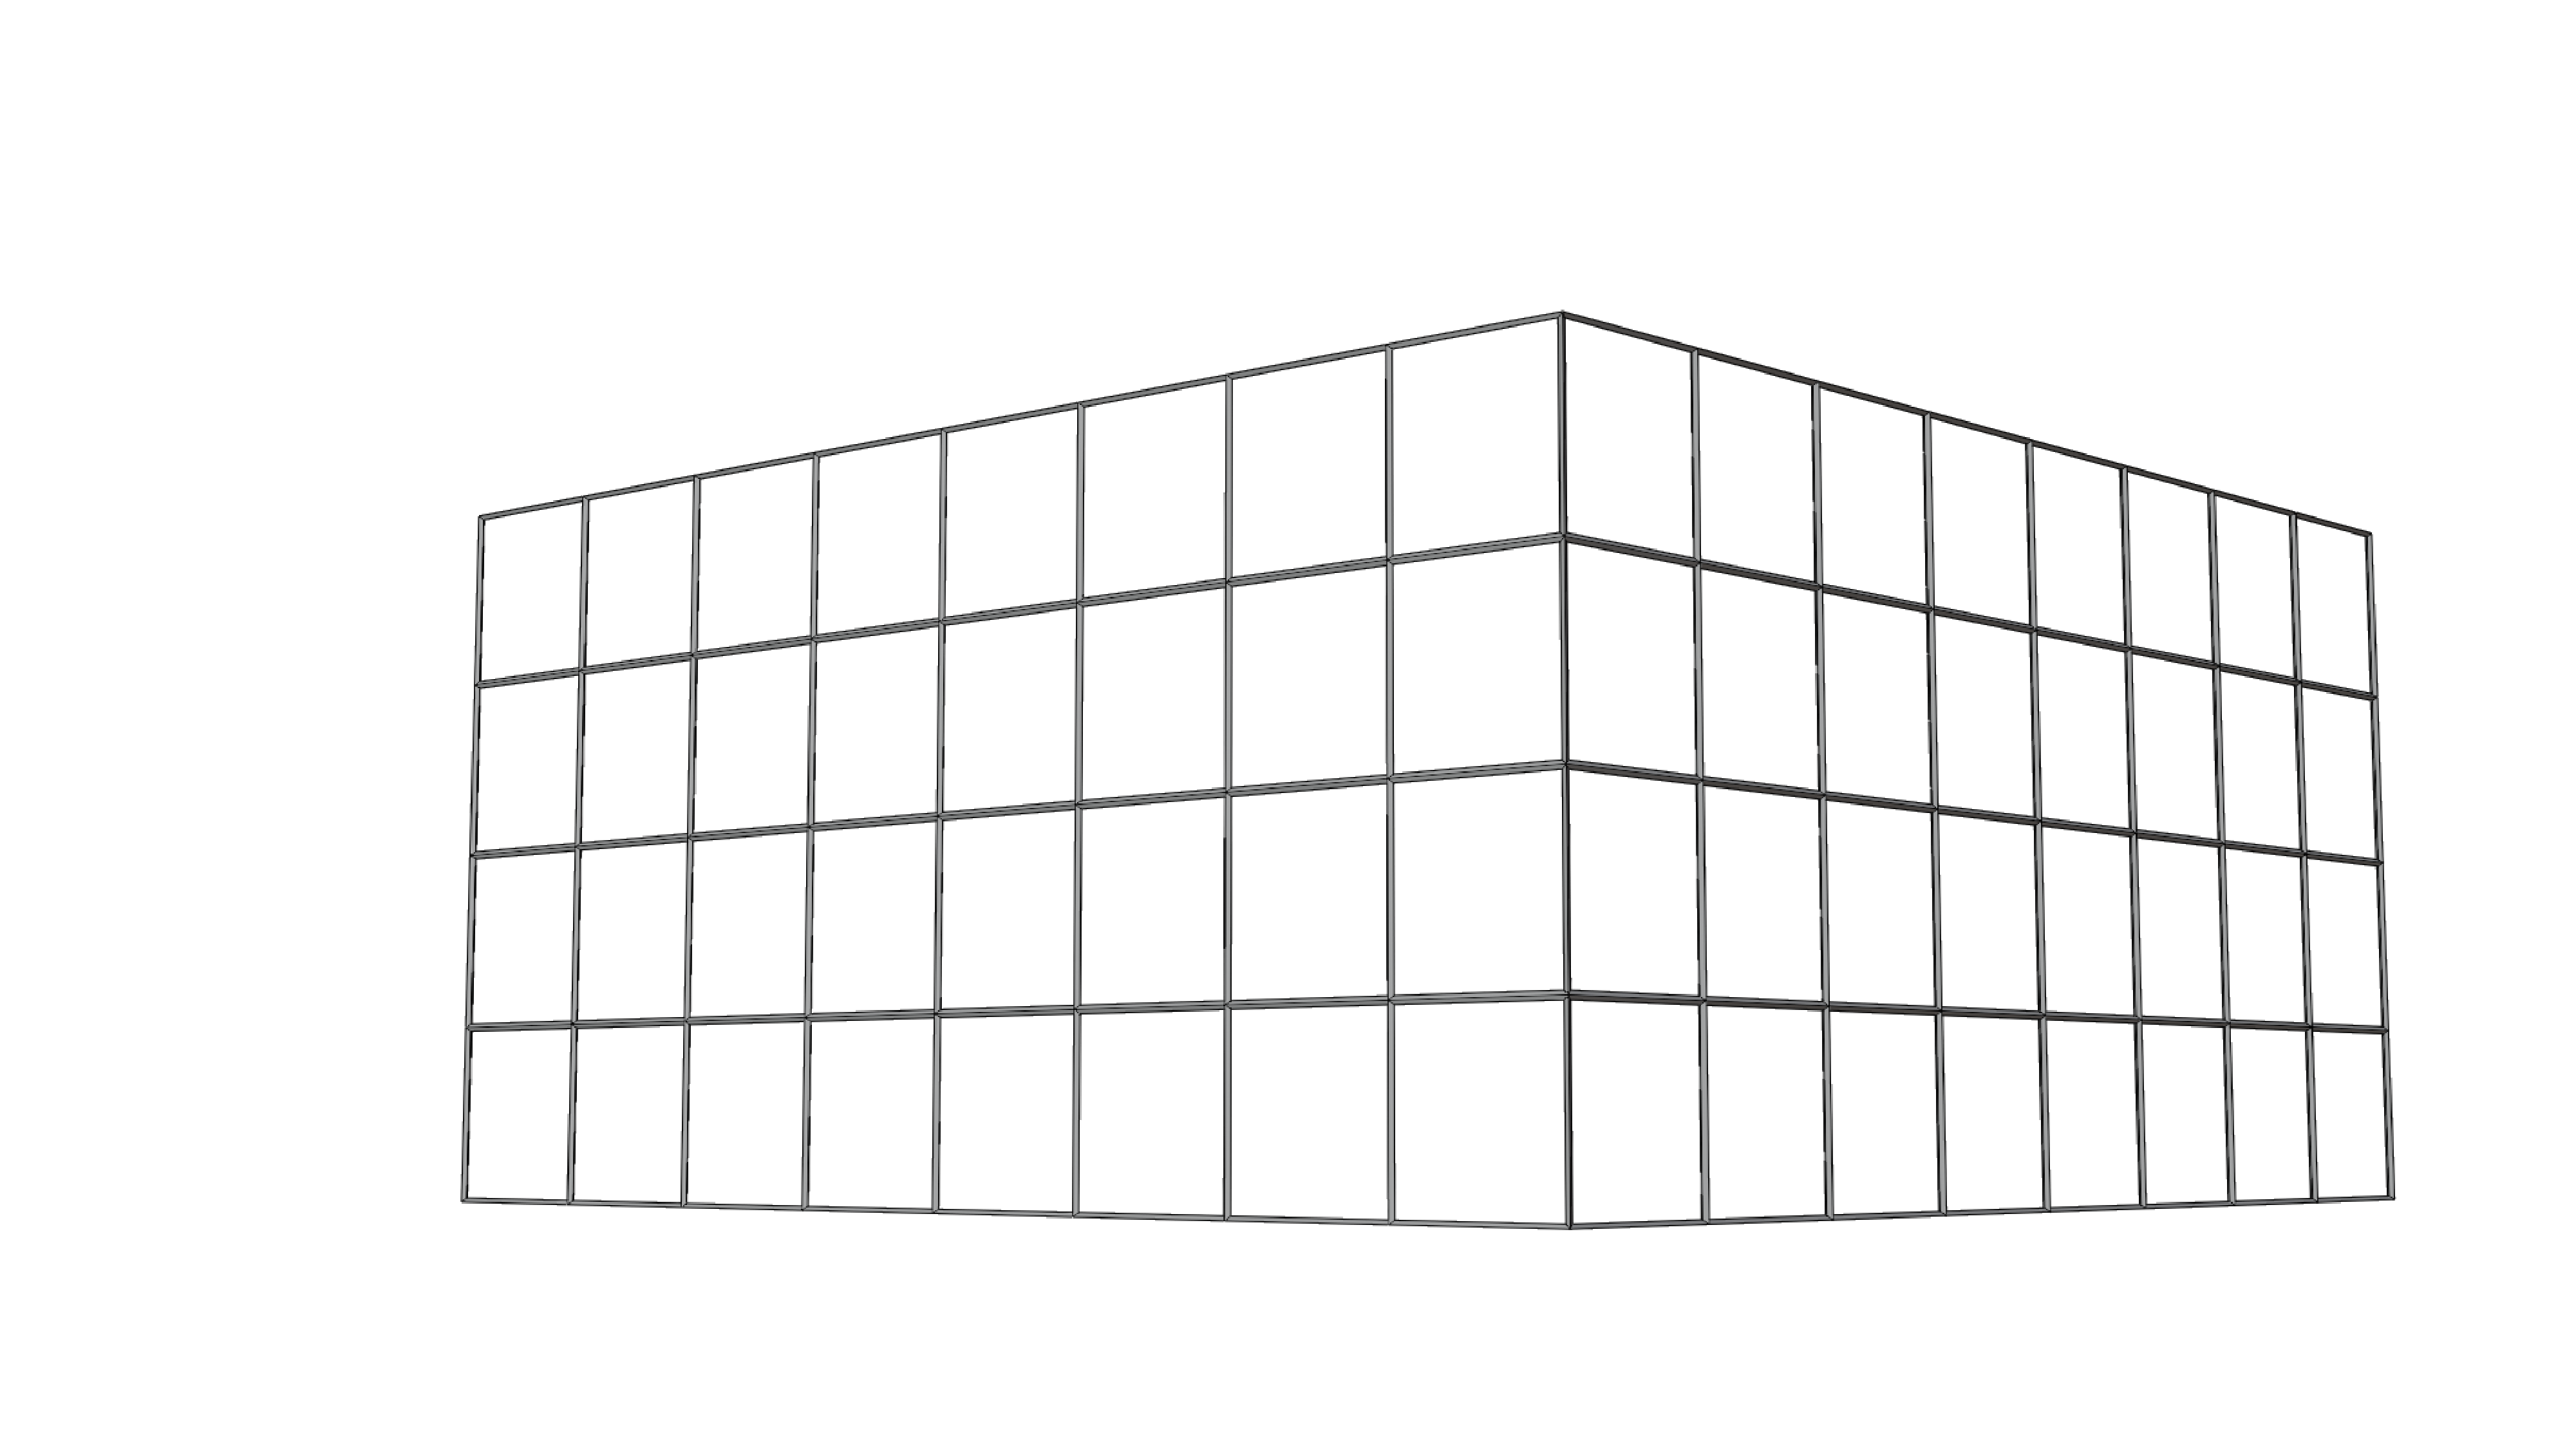
\includegraphics[width=1\linewidth]{Images/Wall 0/0003}} &
              {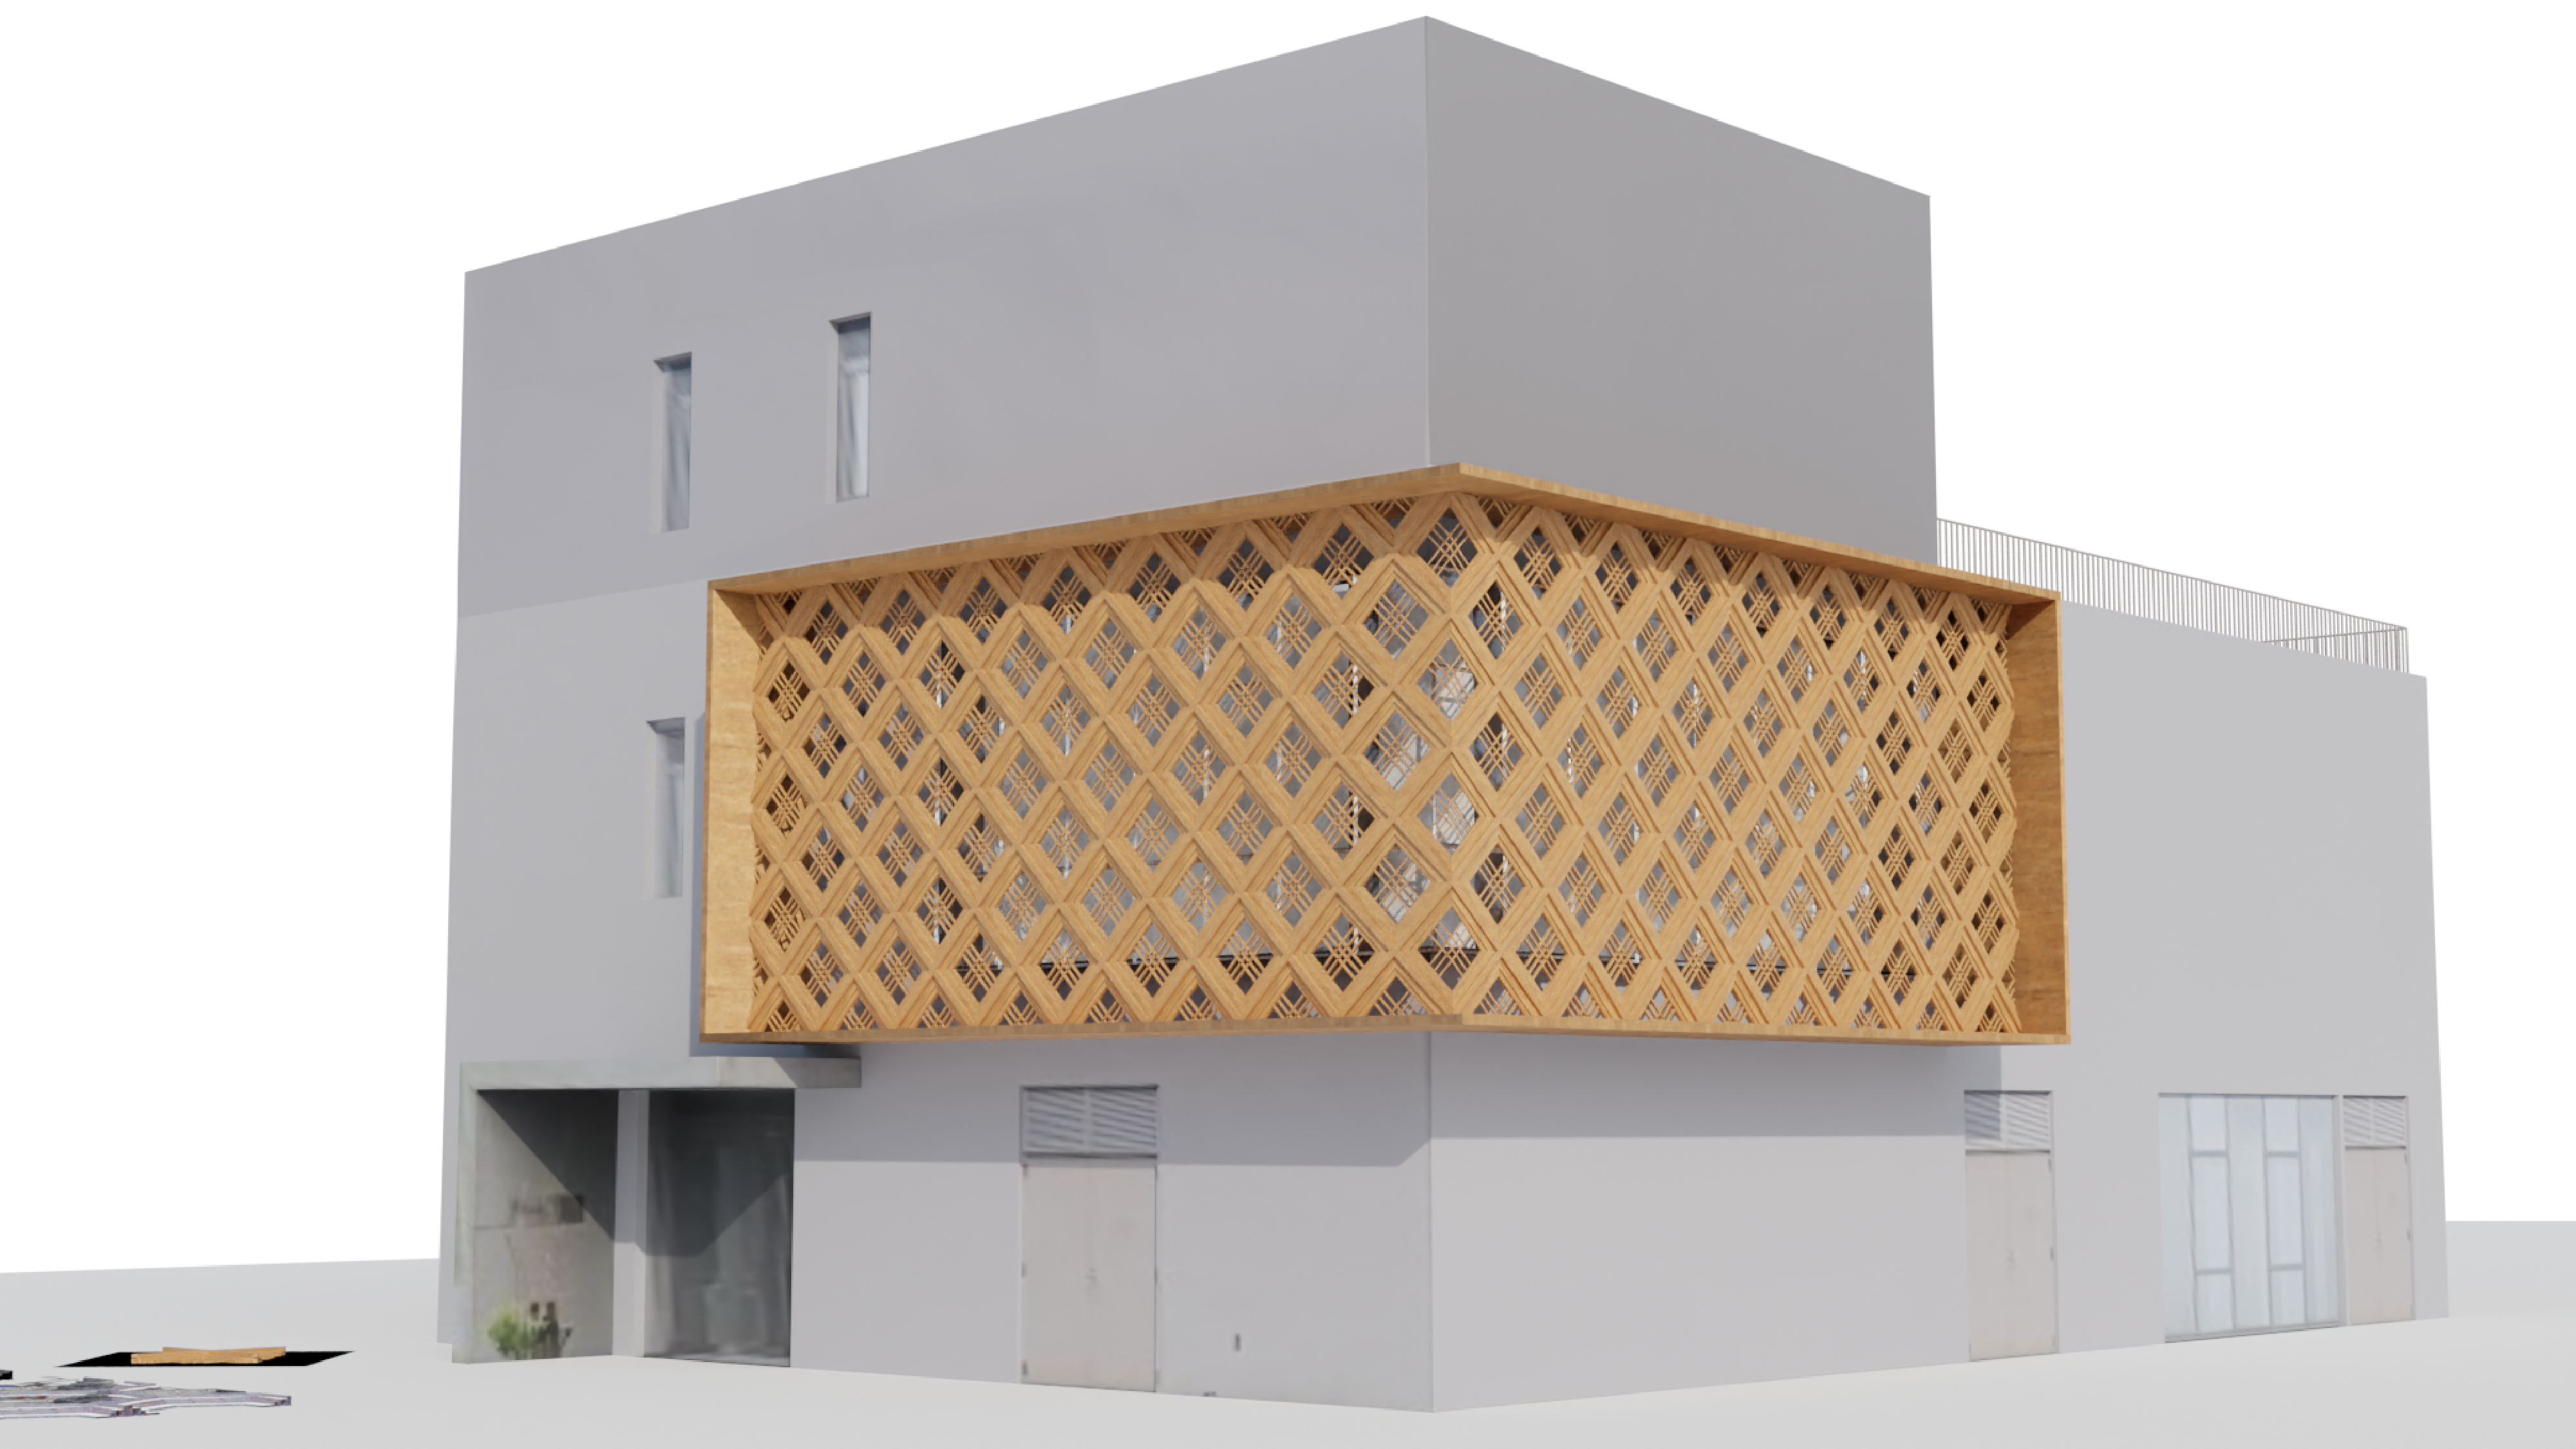
\includegraphics[width=1\linewidth]{Images/Pattern 1/0003}} &
              {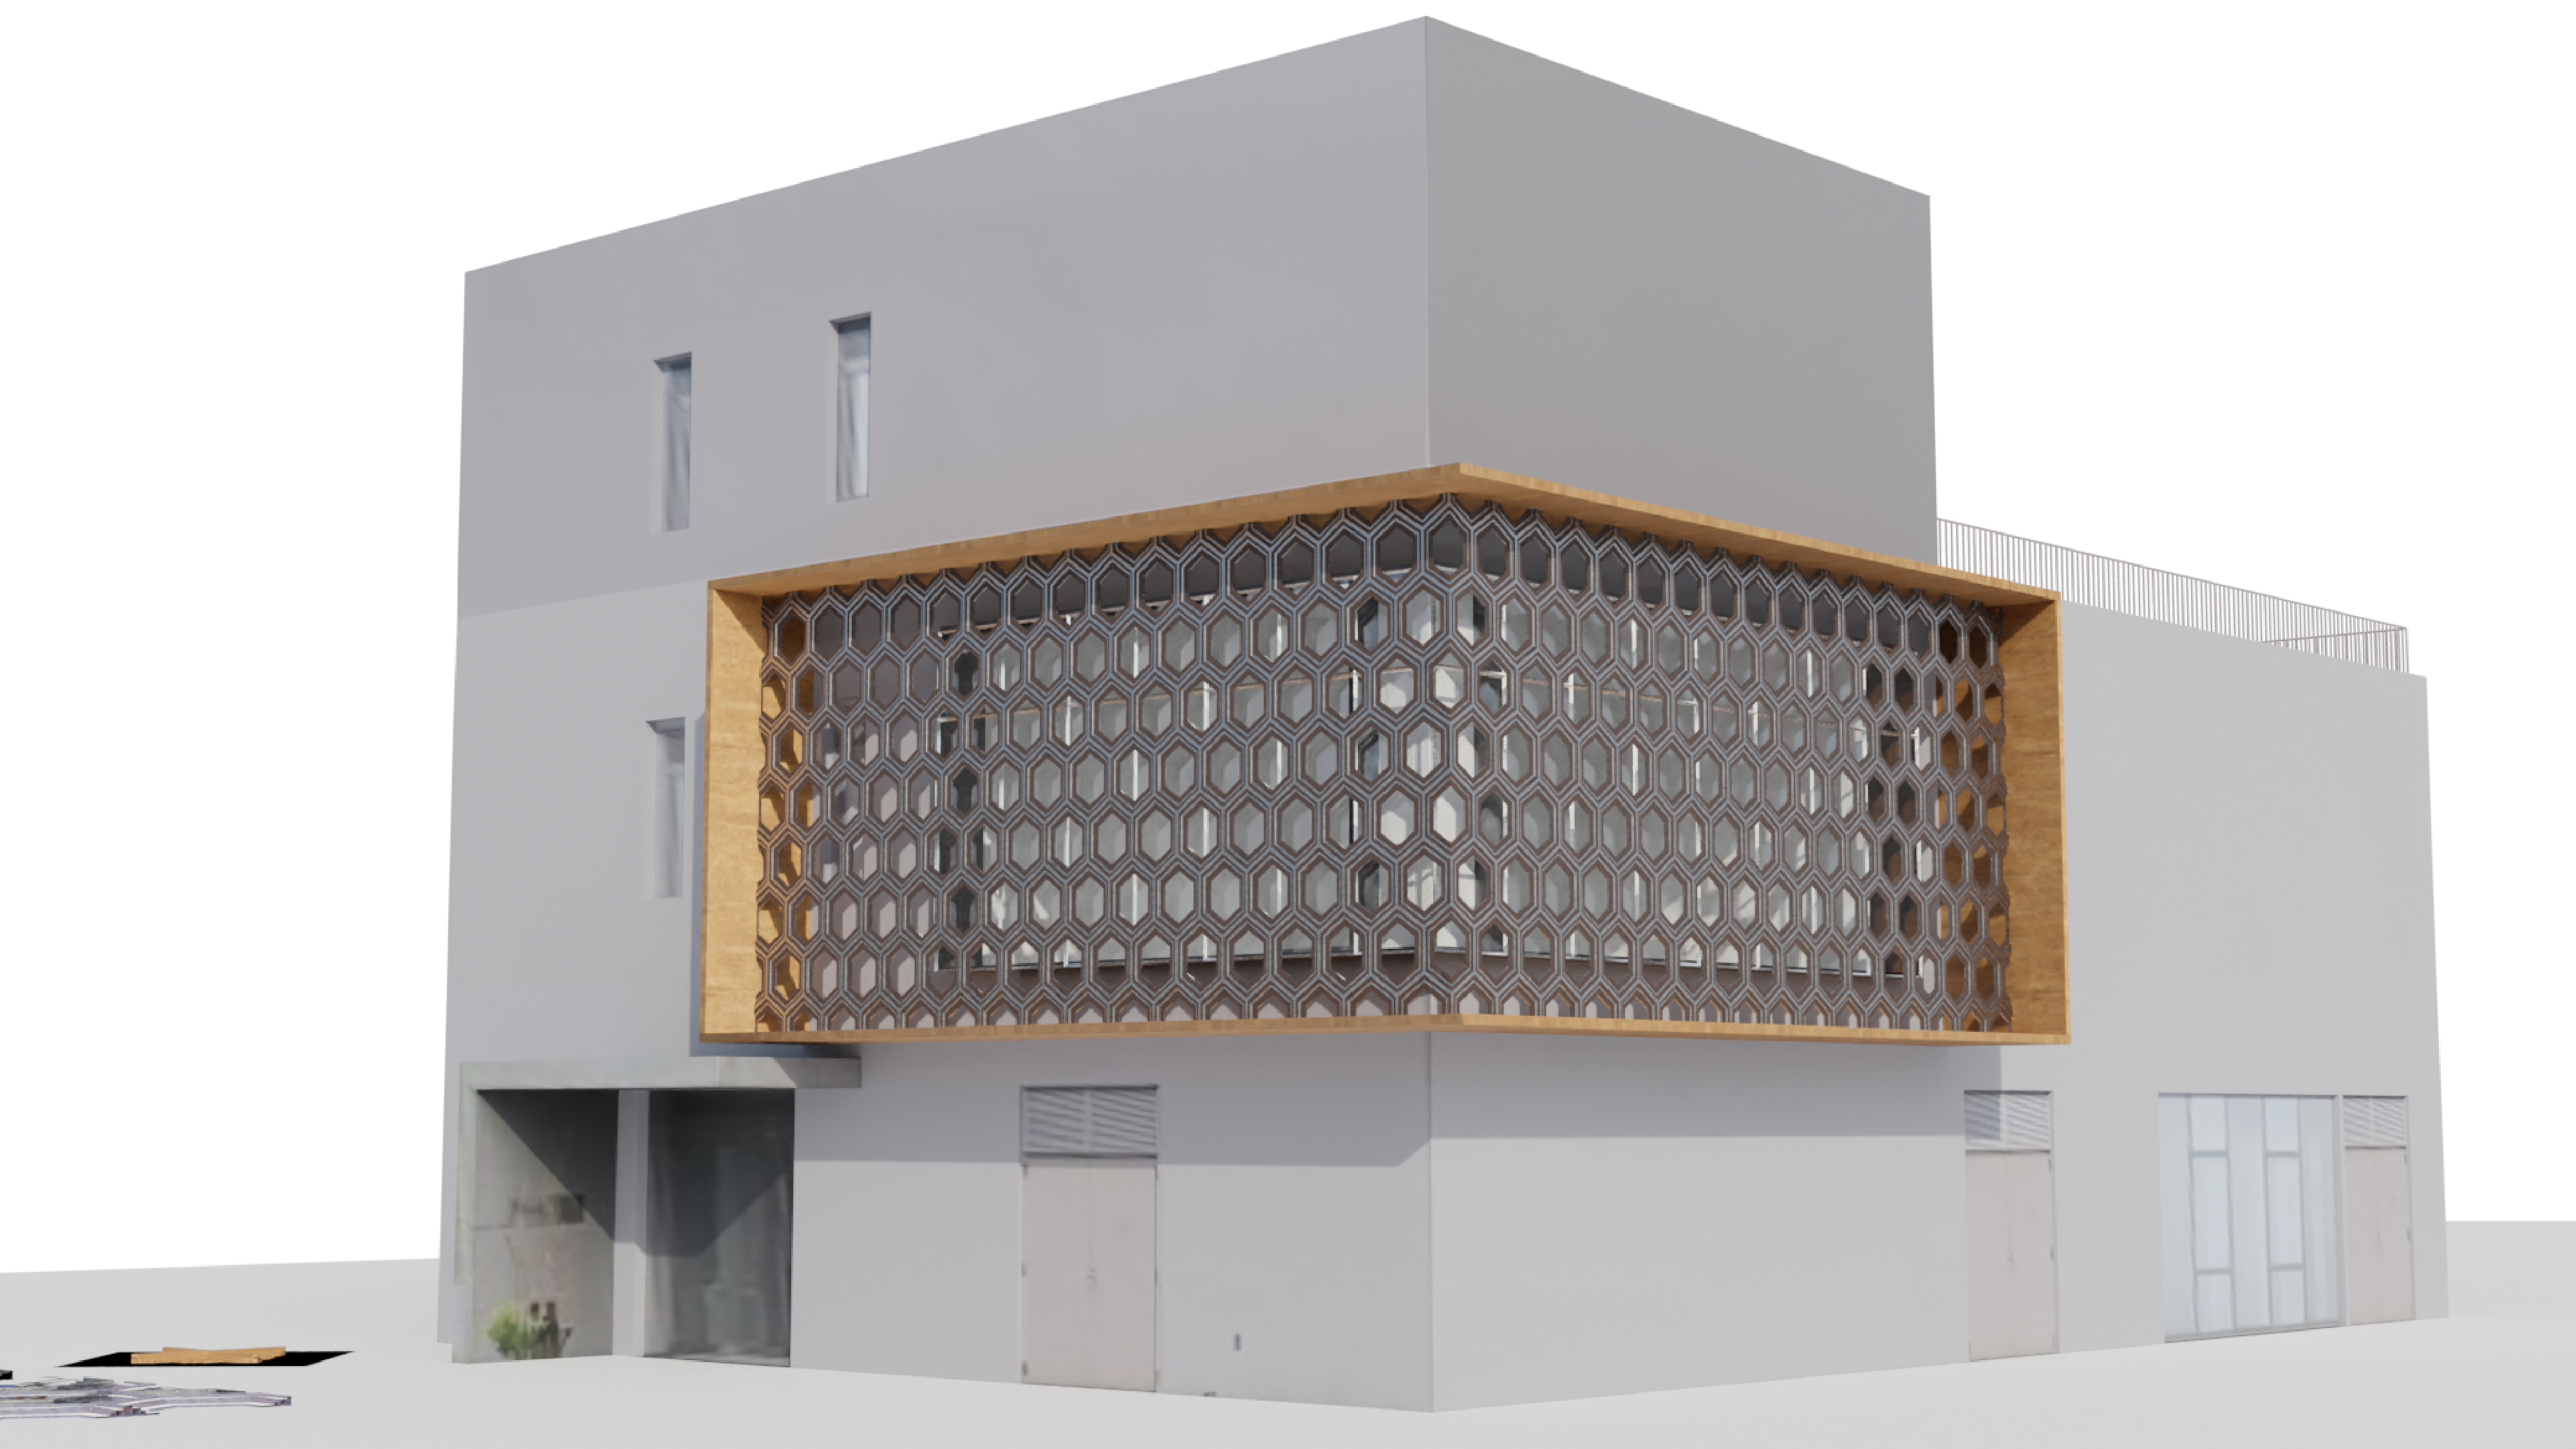
\includegraphics[width=1\linewidth]{Images/Pattern 2/0003}} &
              {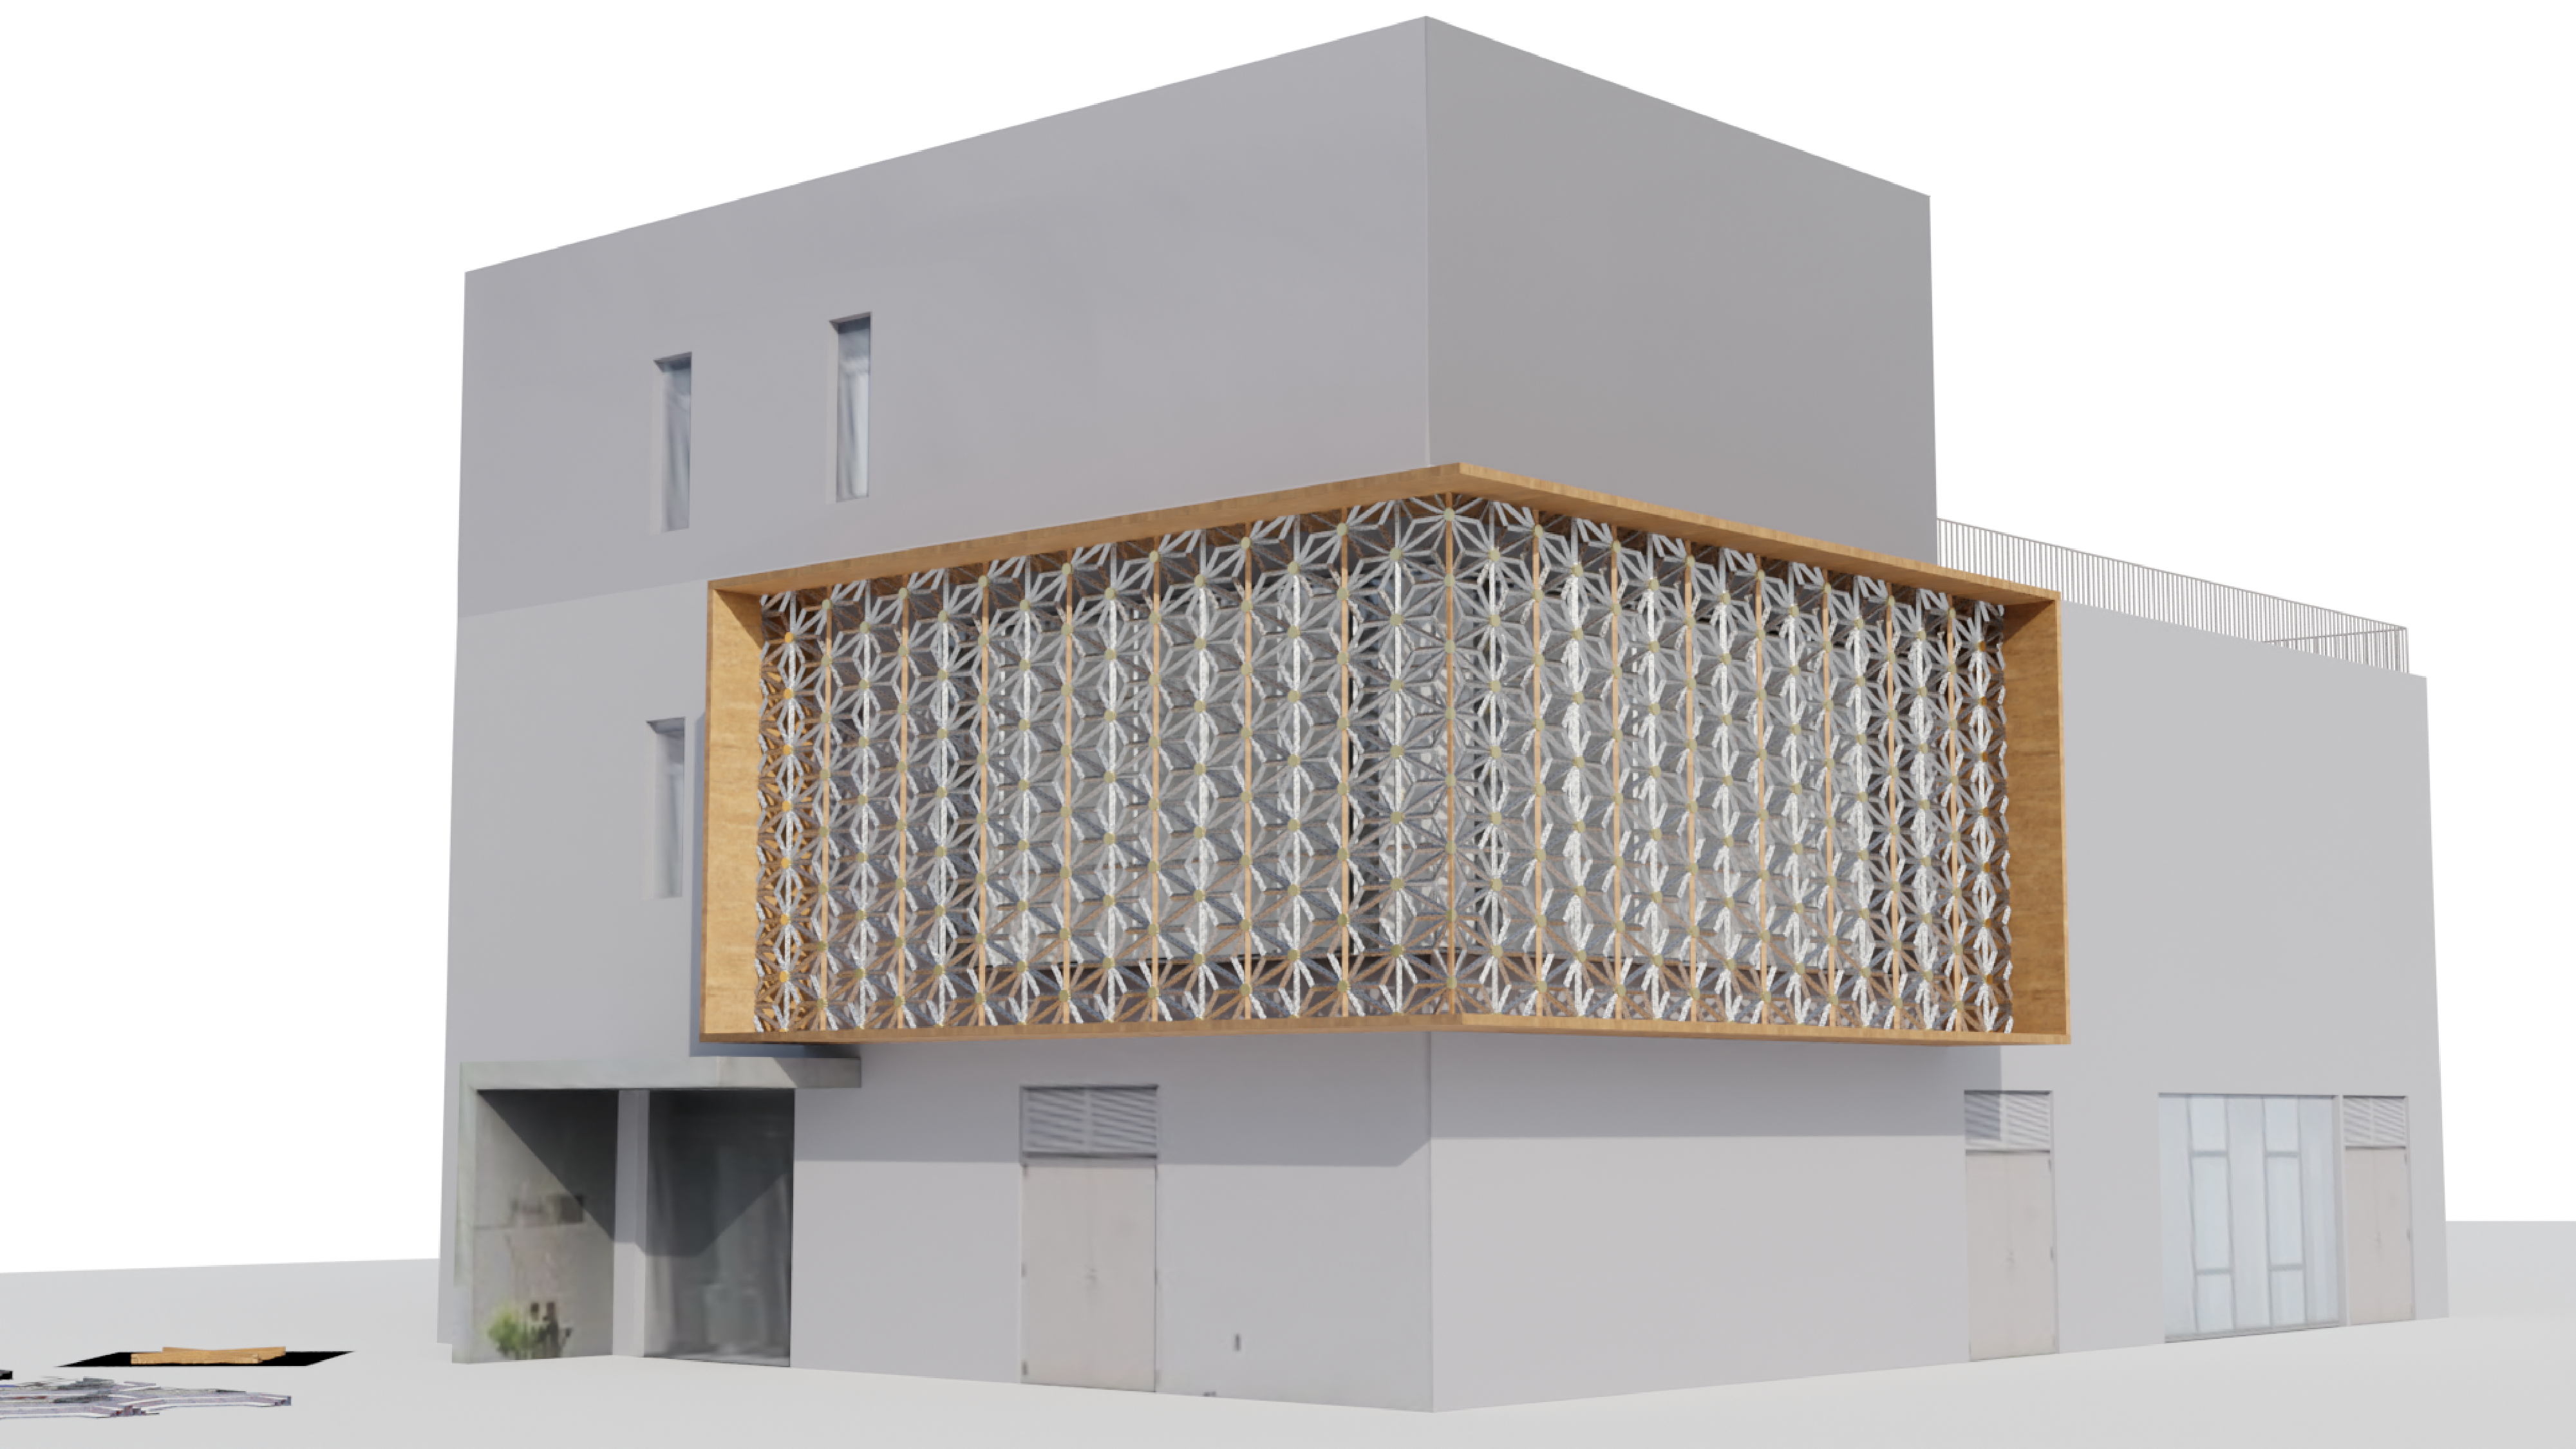
\includegraphics[width=1\linewidth]{Images/Pattern 3/0003}} \\
            \midrule
            \text{Level 6} &  &  &
            \\
            {\includegraphics[width=1\linewidth]{Images/Wall 0/0006}} &
              {\includegraphics[width=1\linewidth]{Images/Pattern 1/0006}} &
              {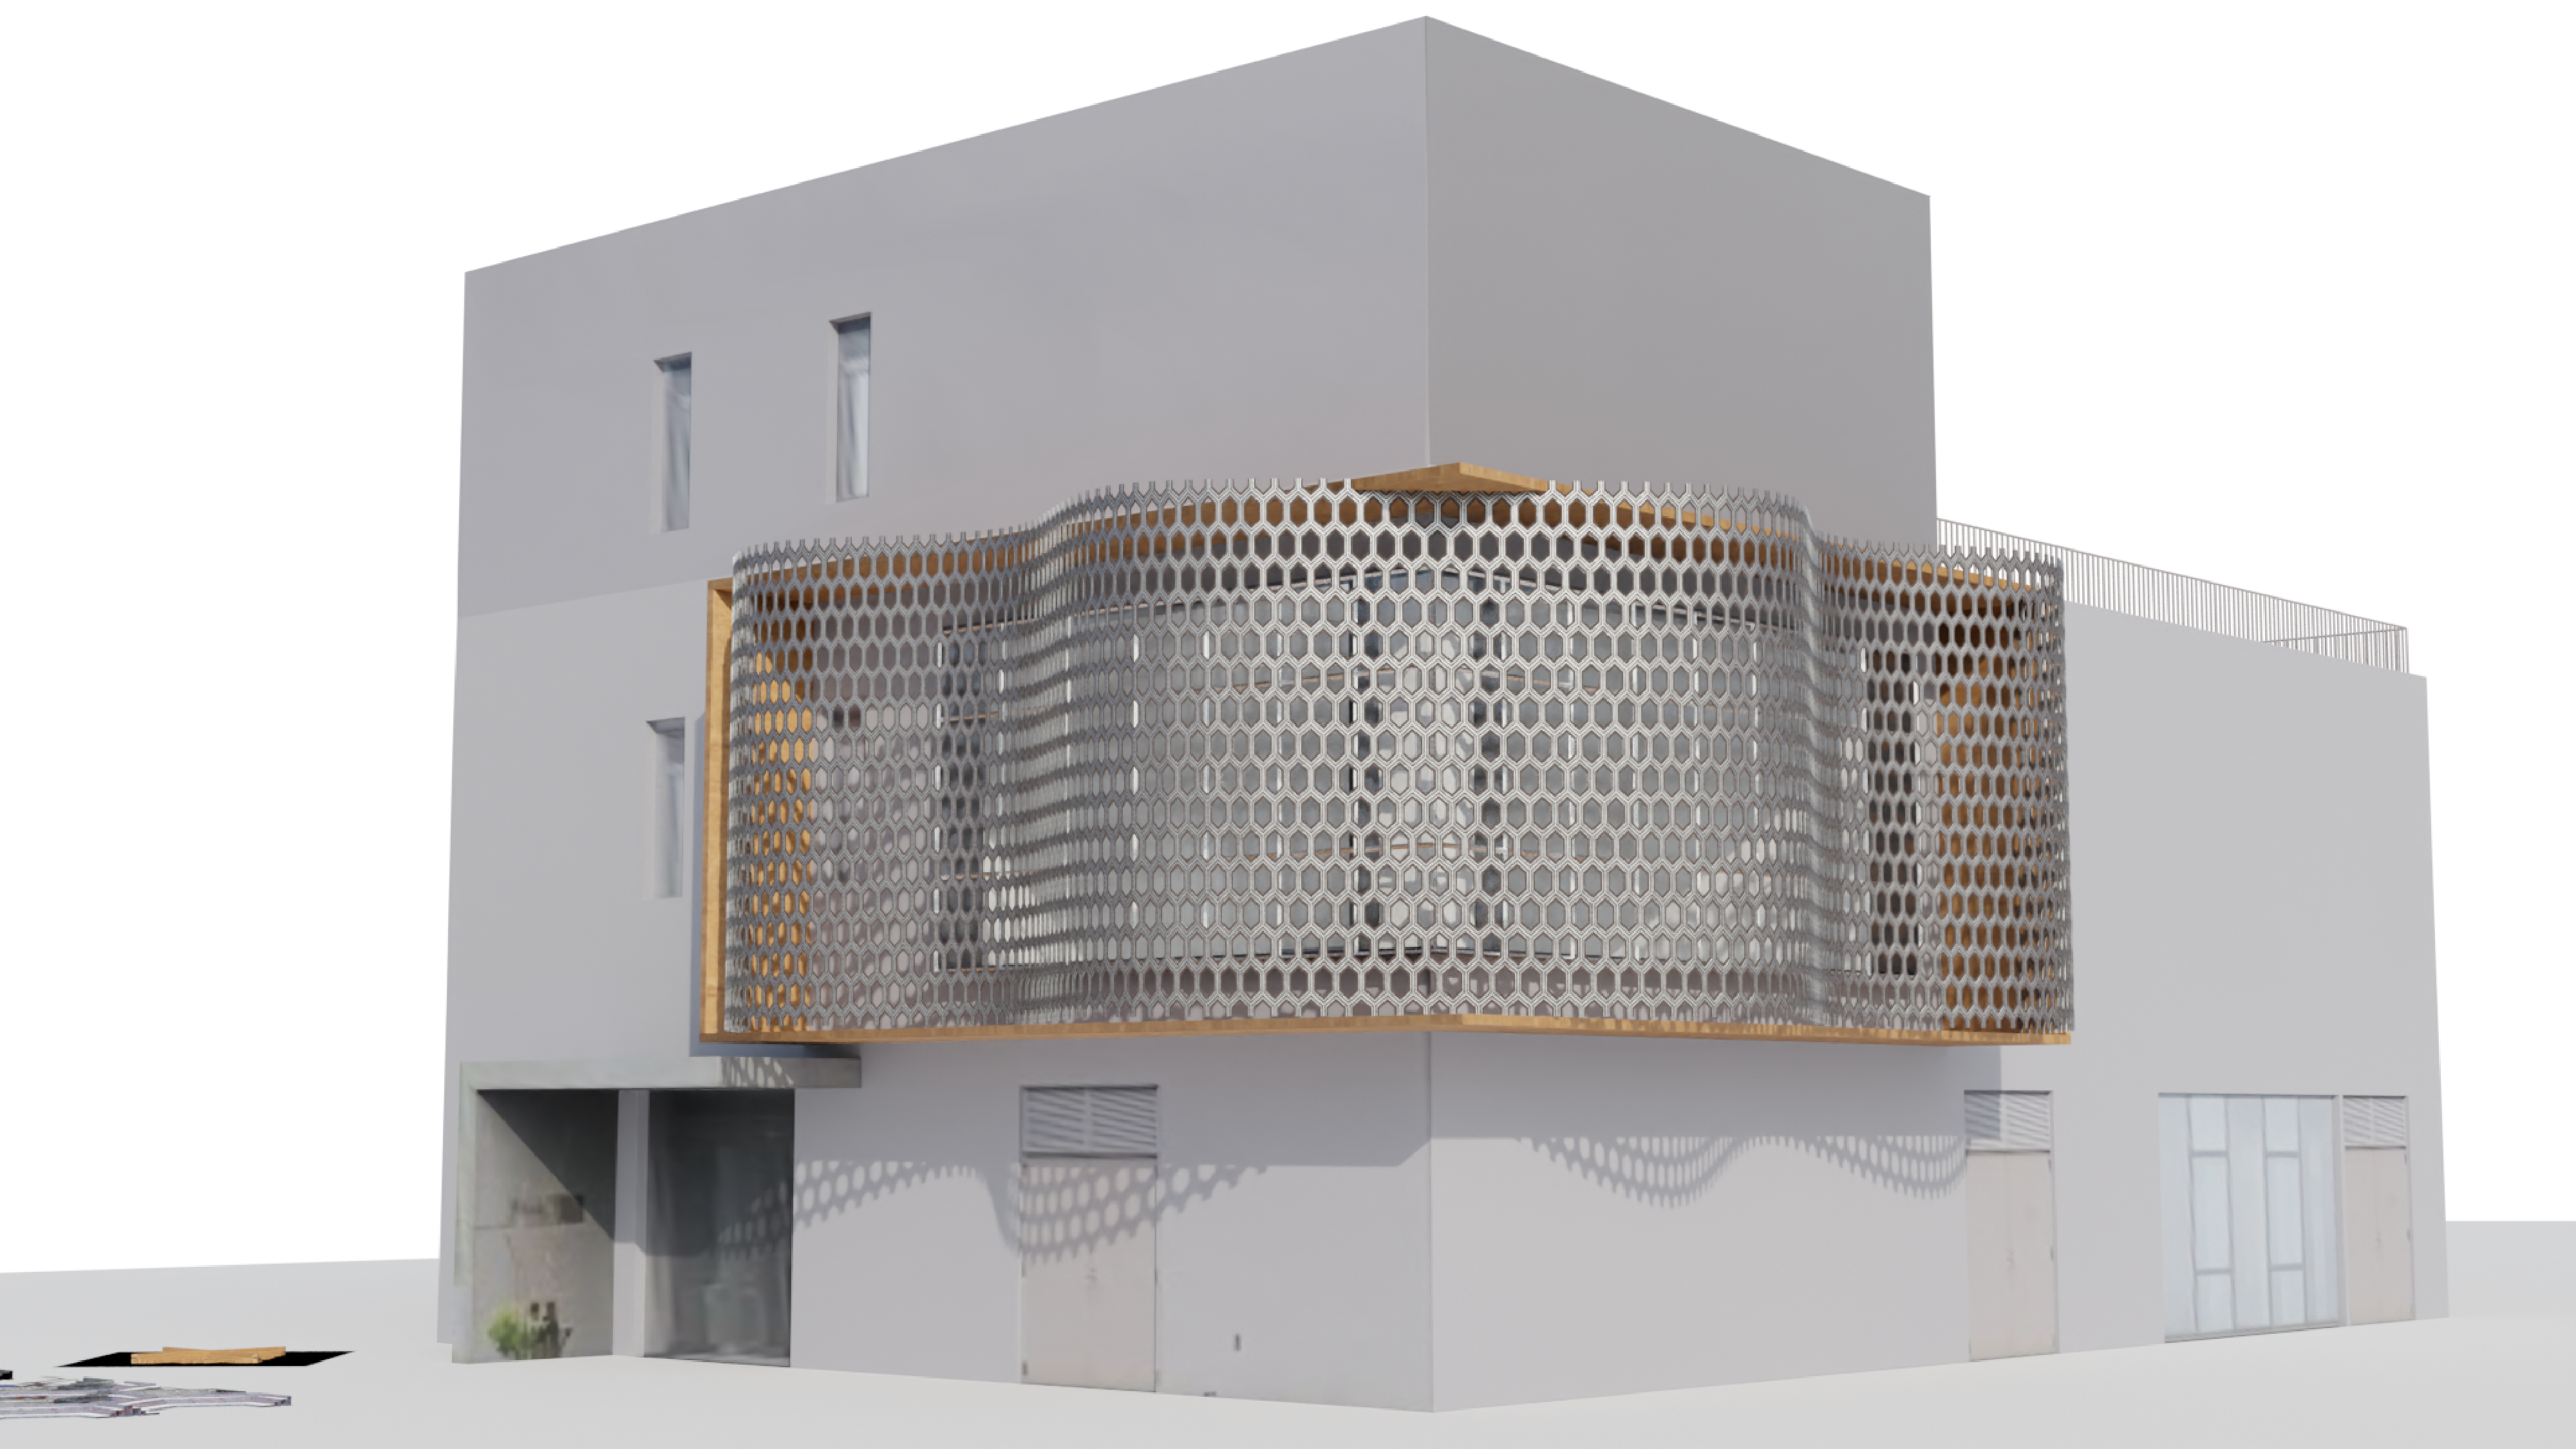
\includegraphics[width=1\linewidth]{Images/Pattern 2/0006}} &
              {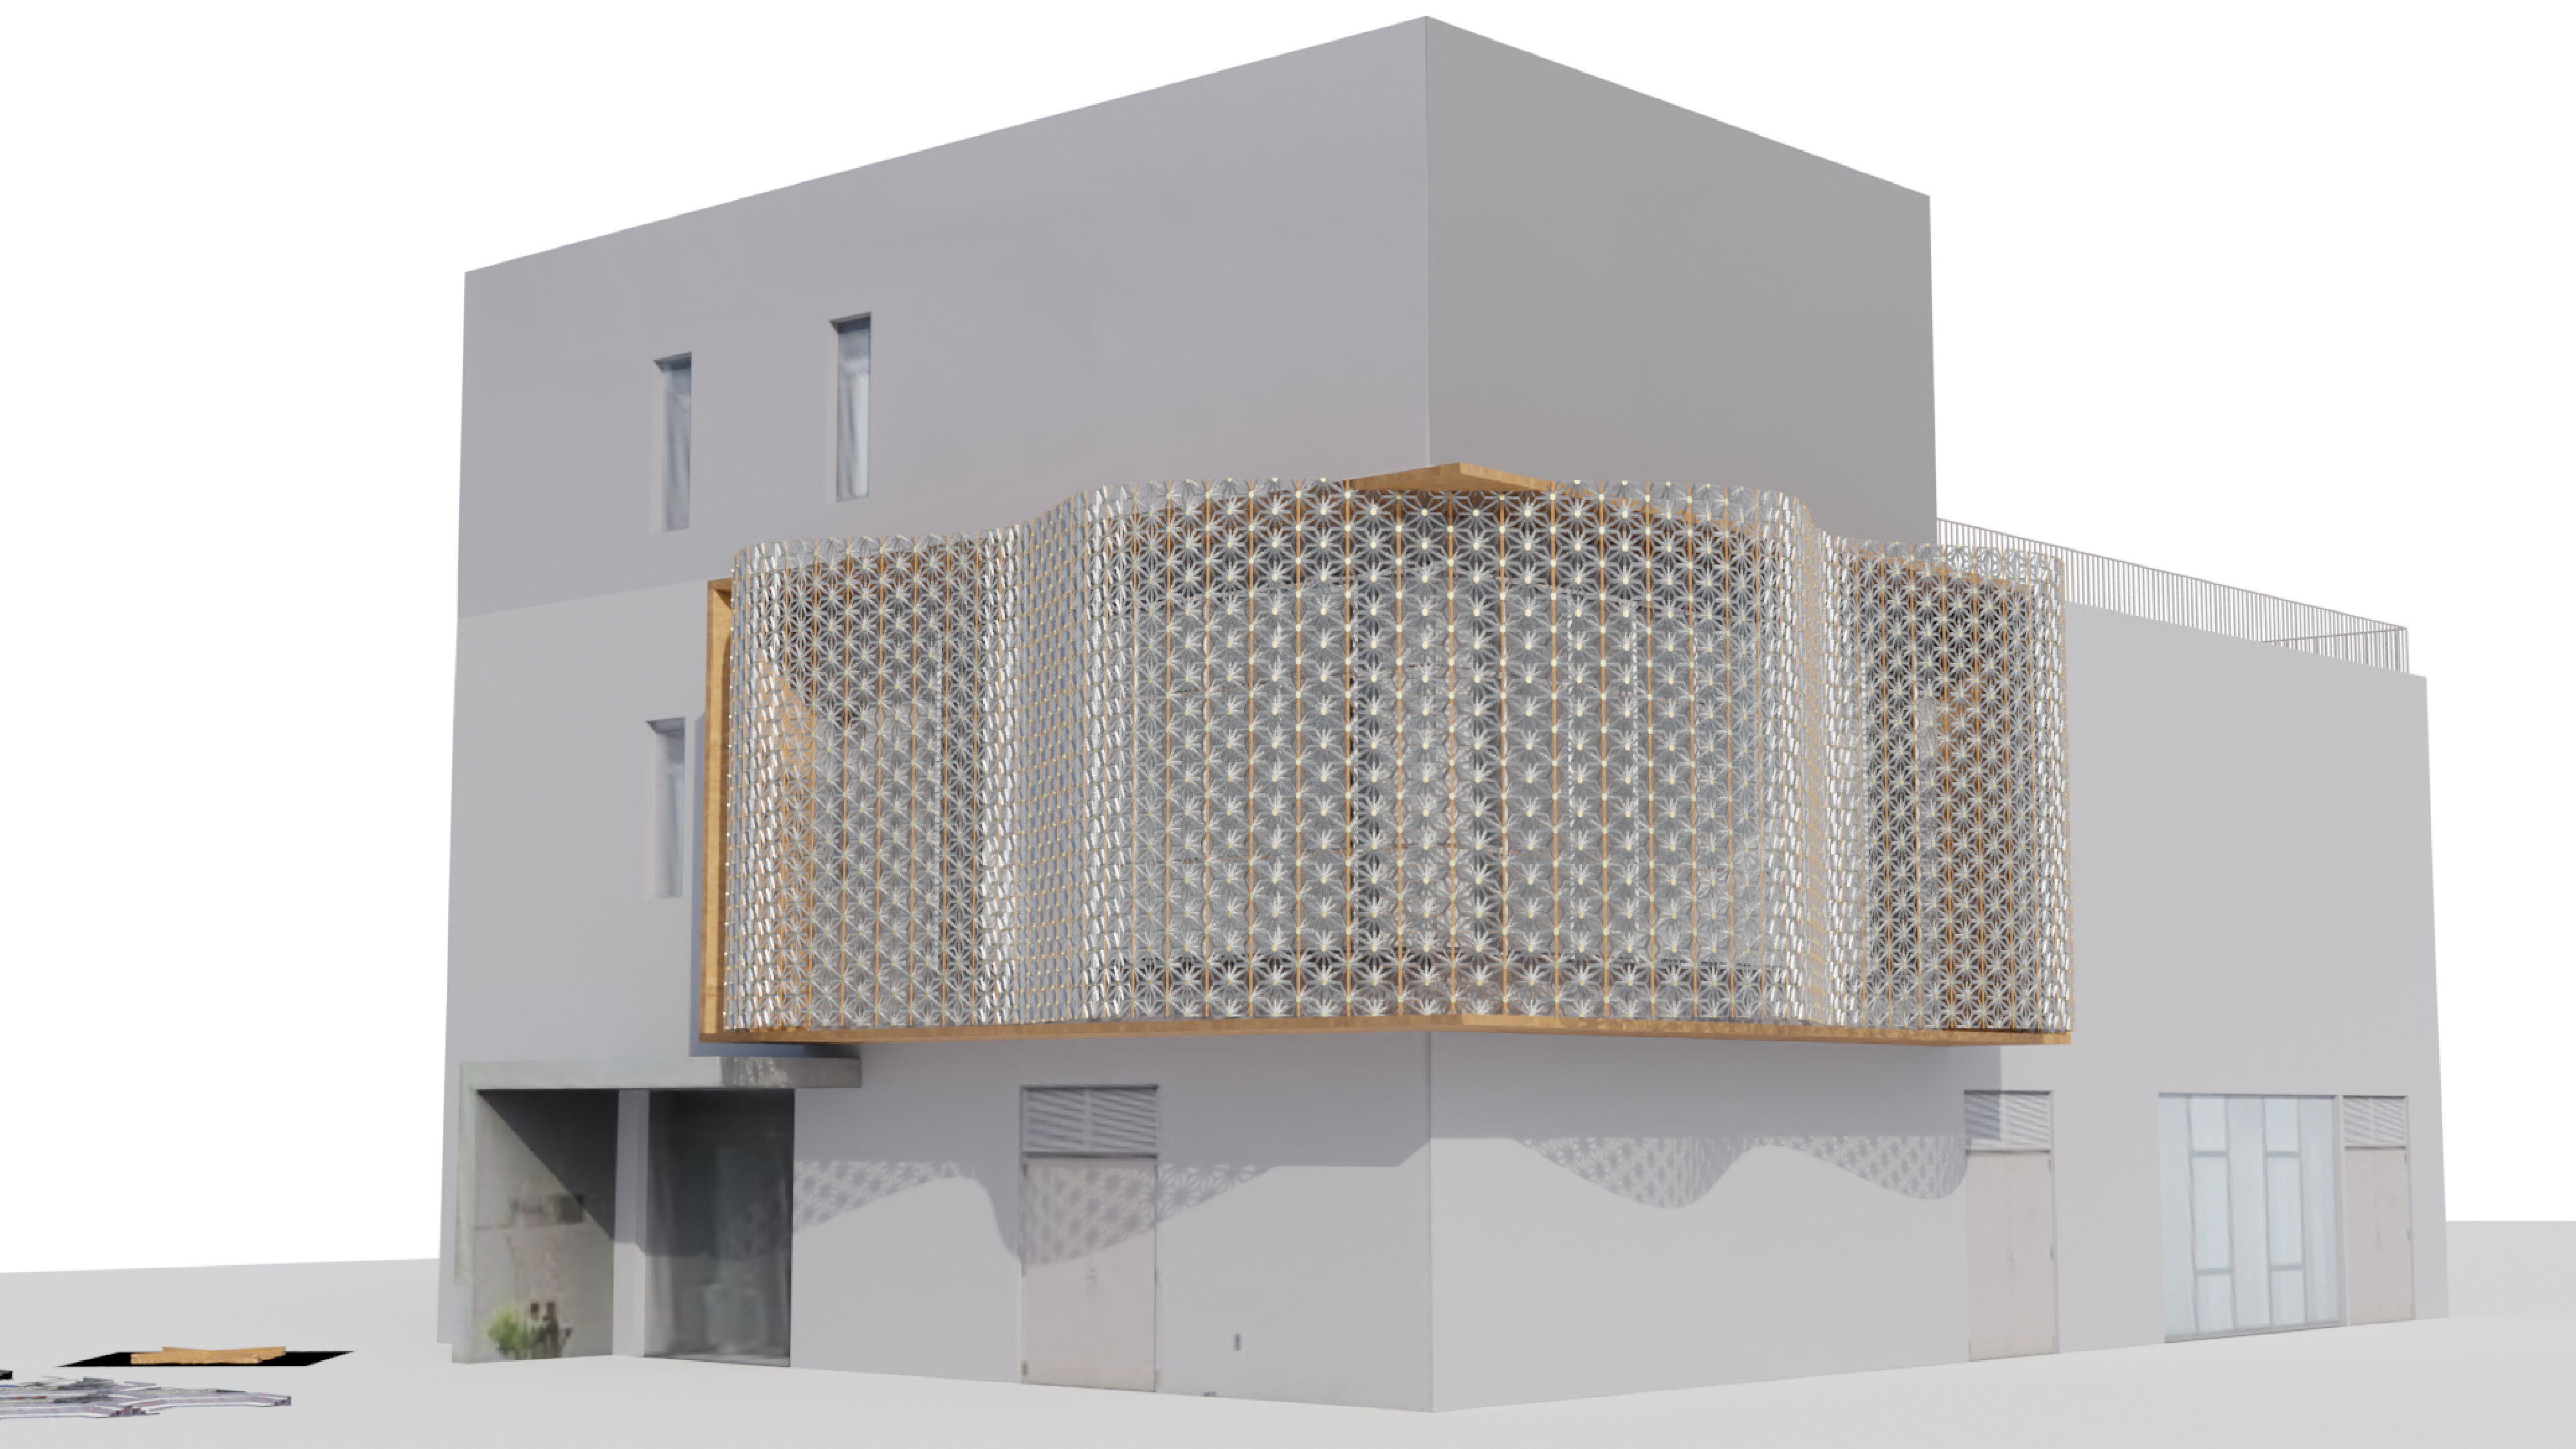
\includegraphics[width=1\linewidth]{Images/Pattern 3/0006}} \\
            \midrule
            \text{Level 9} &  &  &
            \\
            {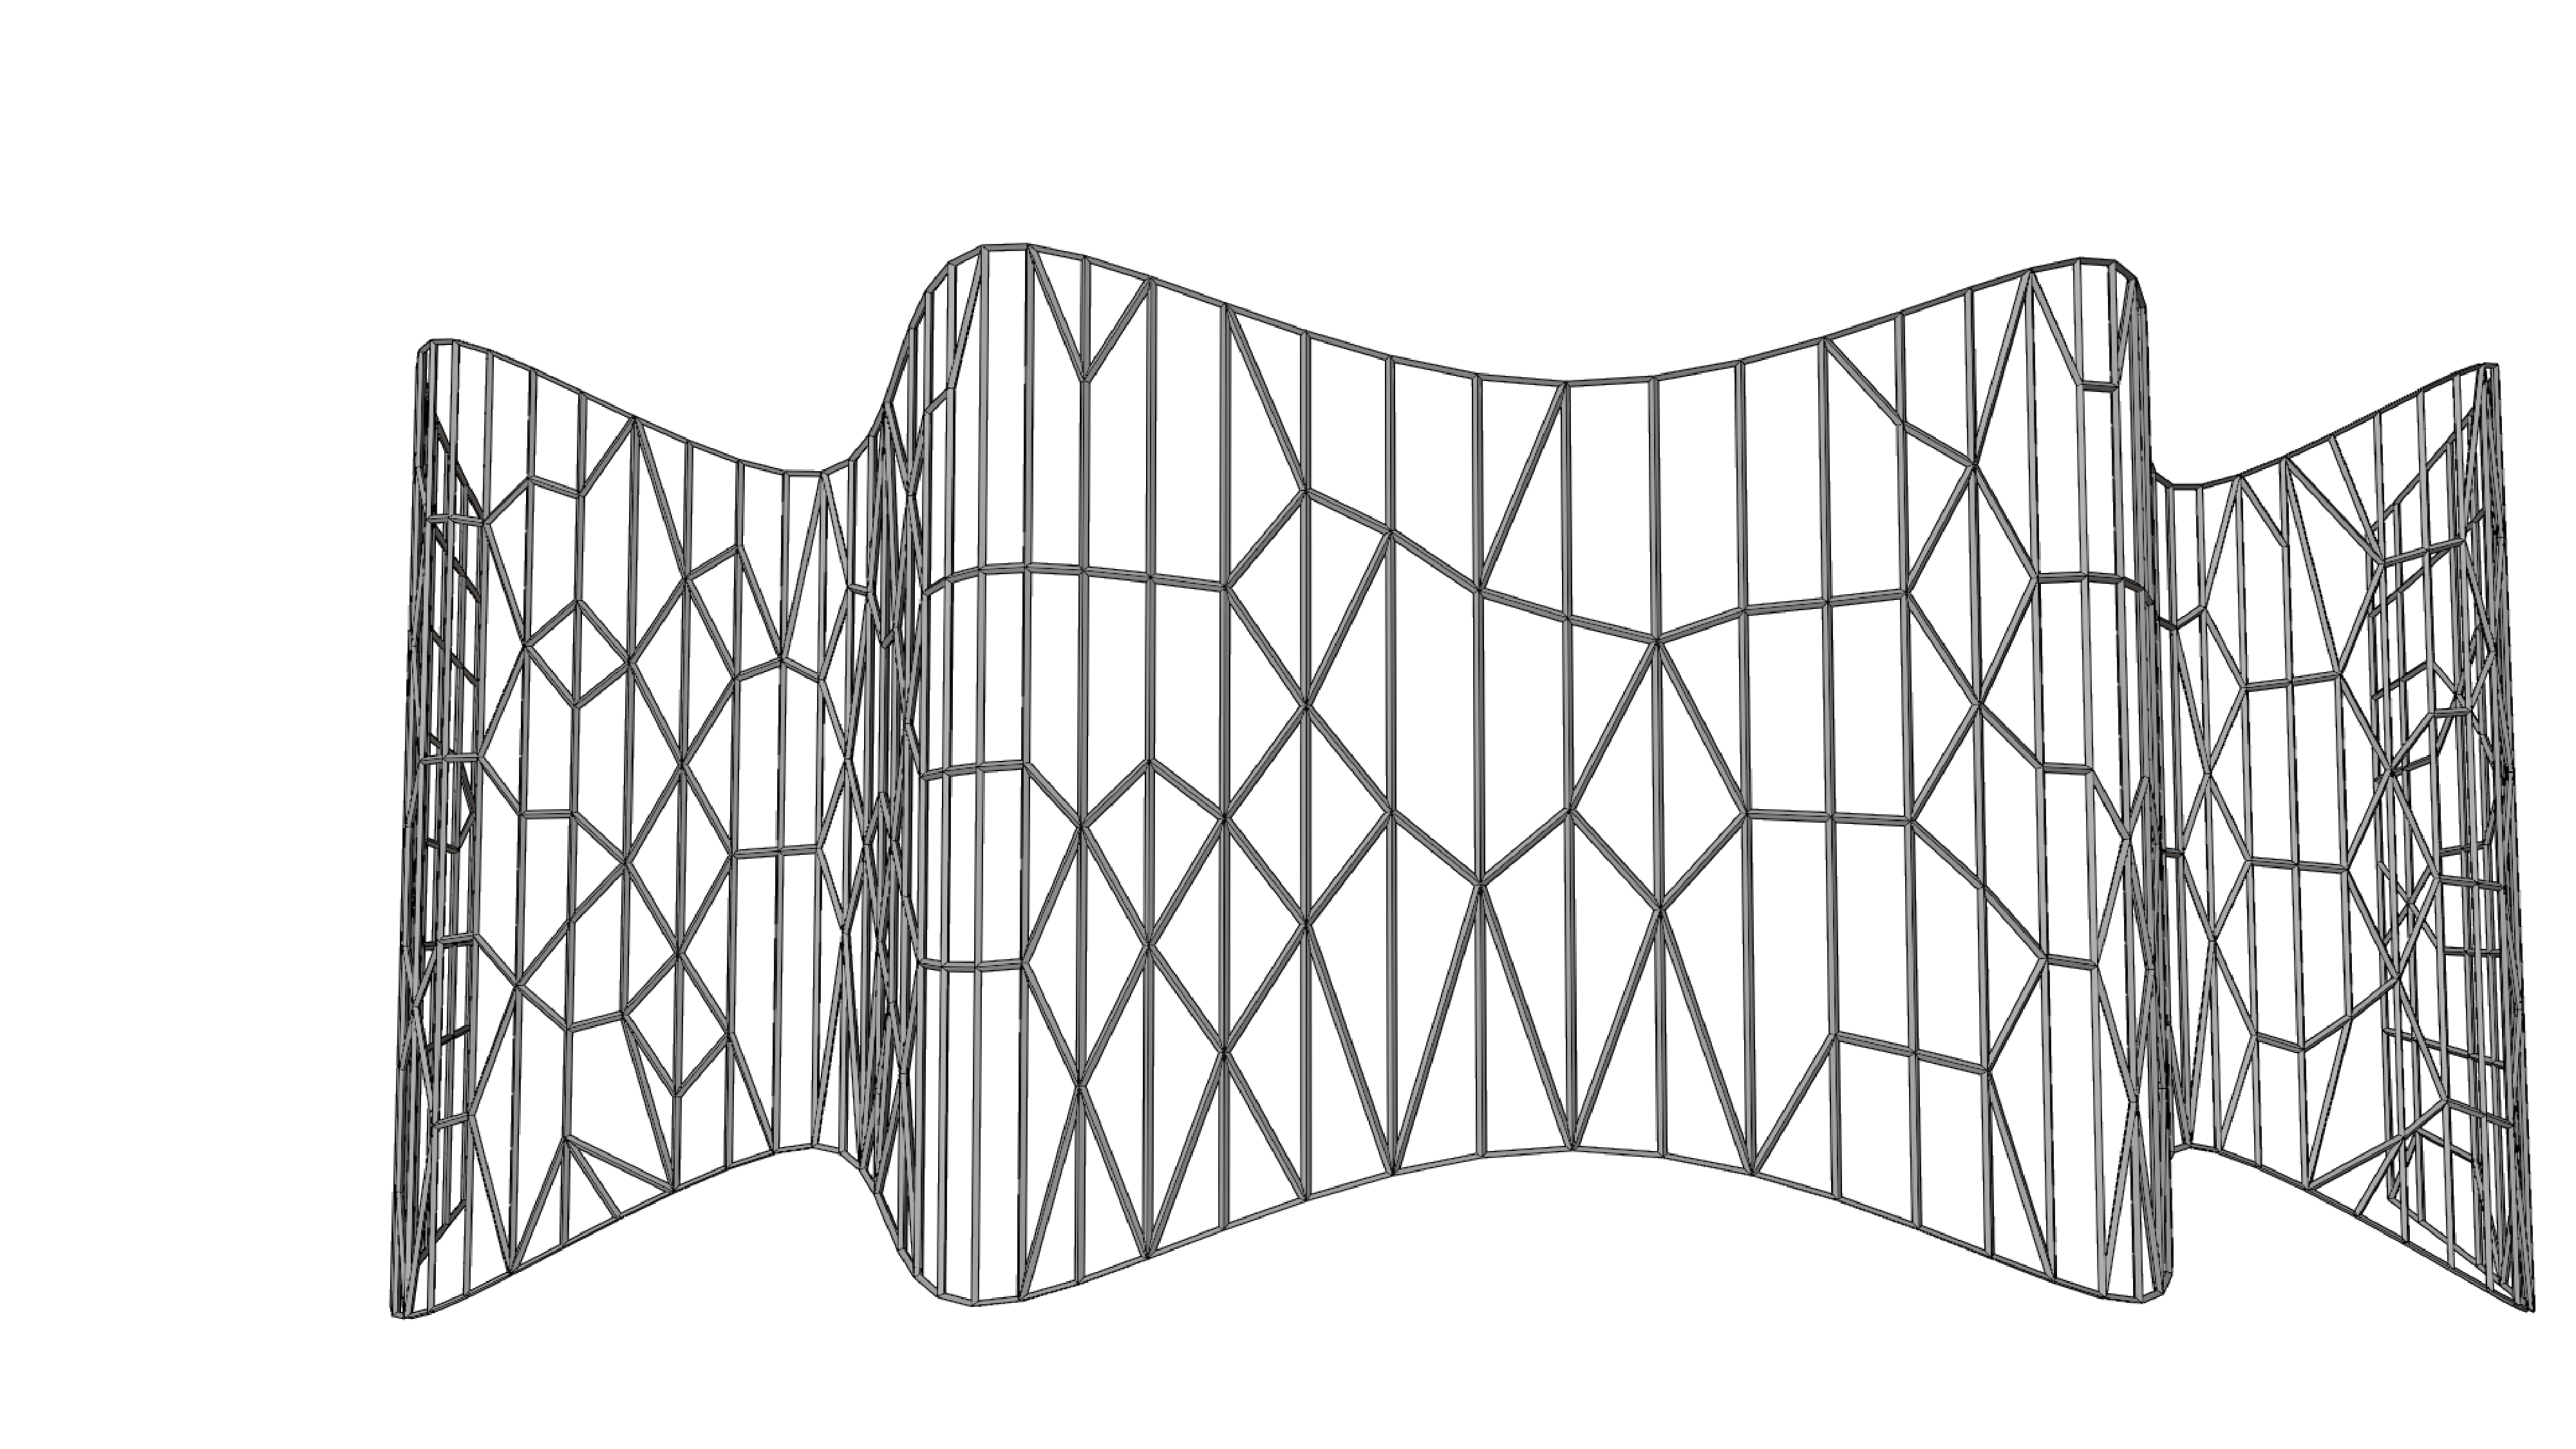
\includegraphics[width=1\linewidth]{Images/Wall 0/0009}} &
              {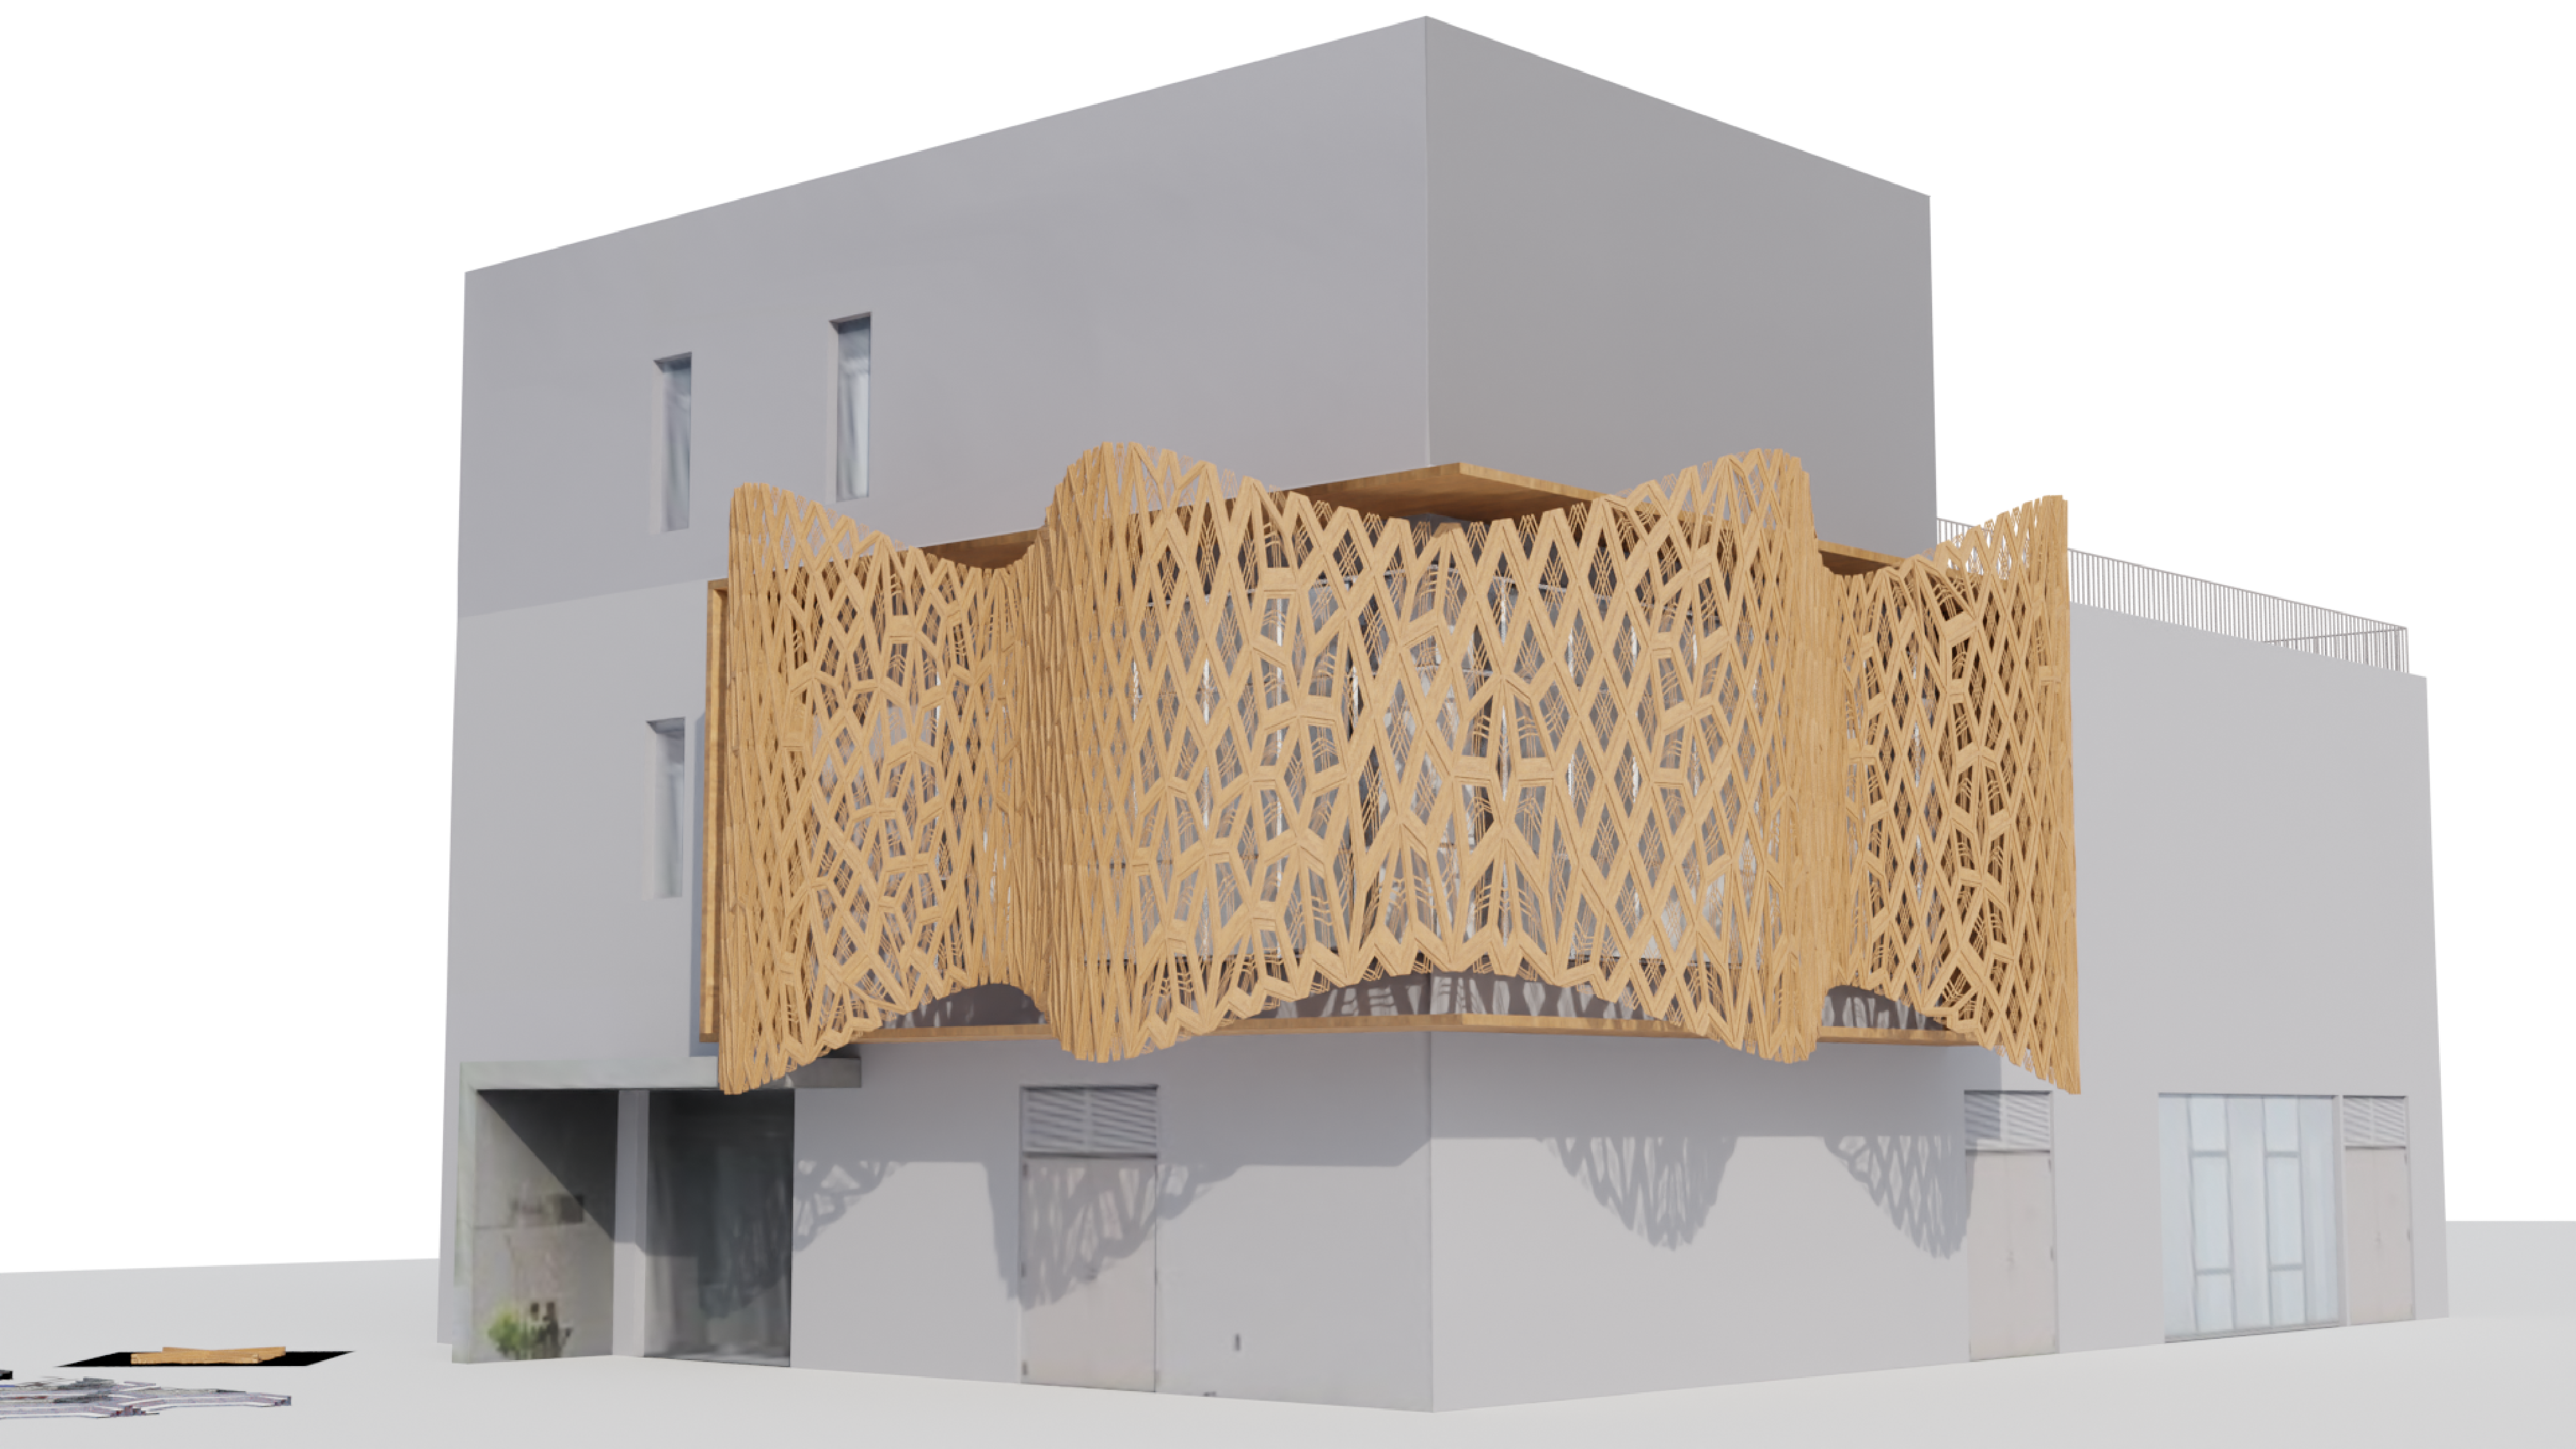
\includegraphics[width=1\linewidth]{Images/Pattern 1/0009}} &
              {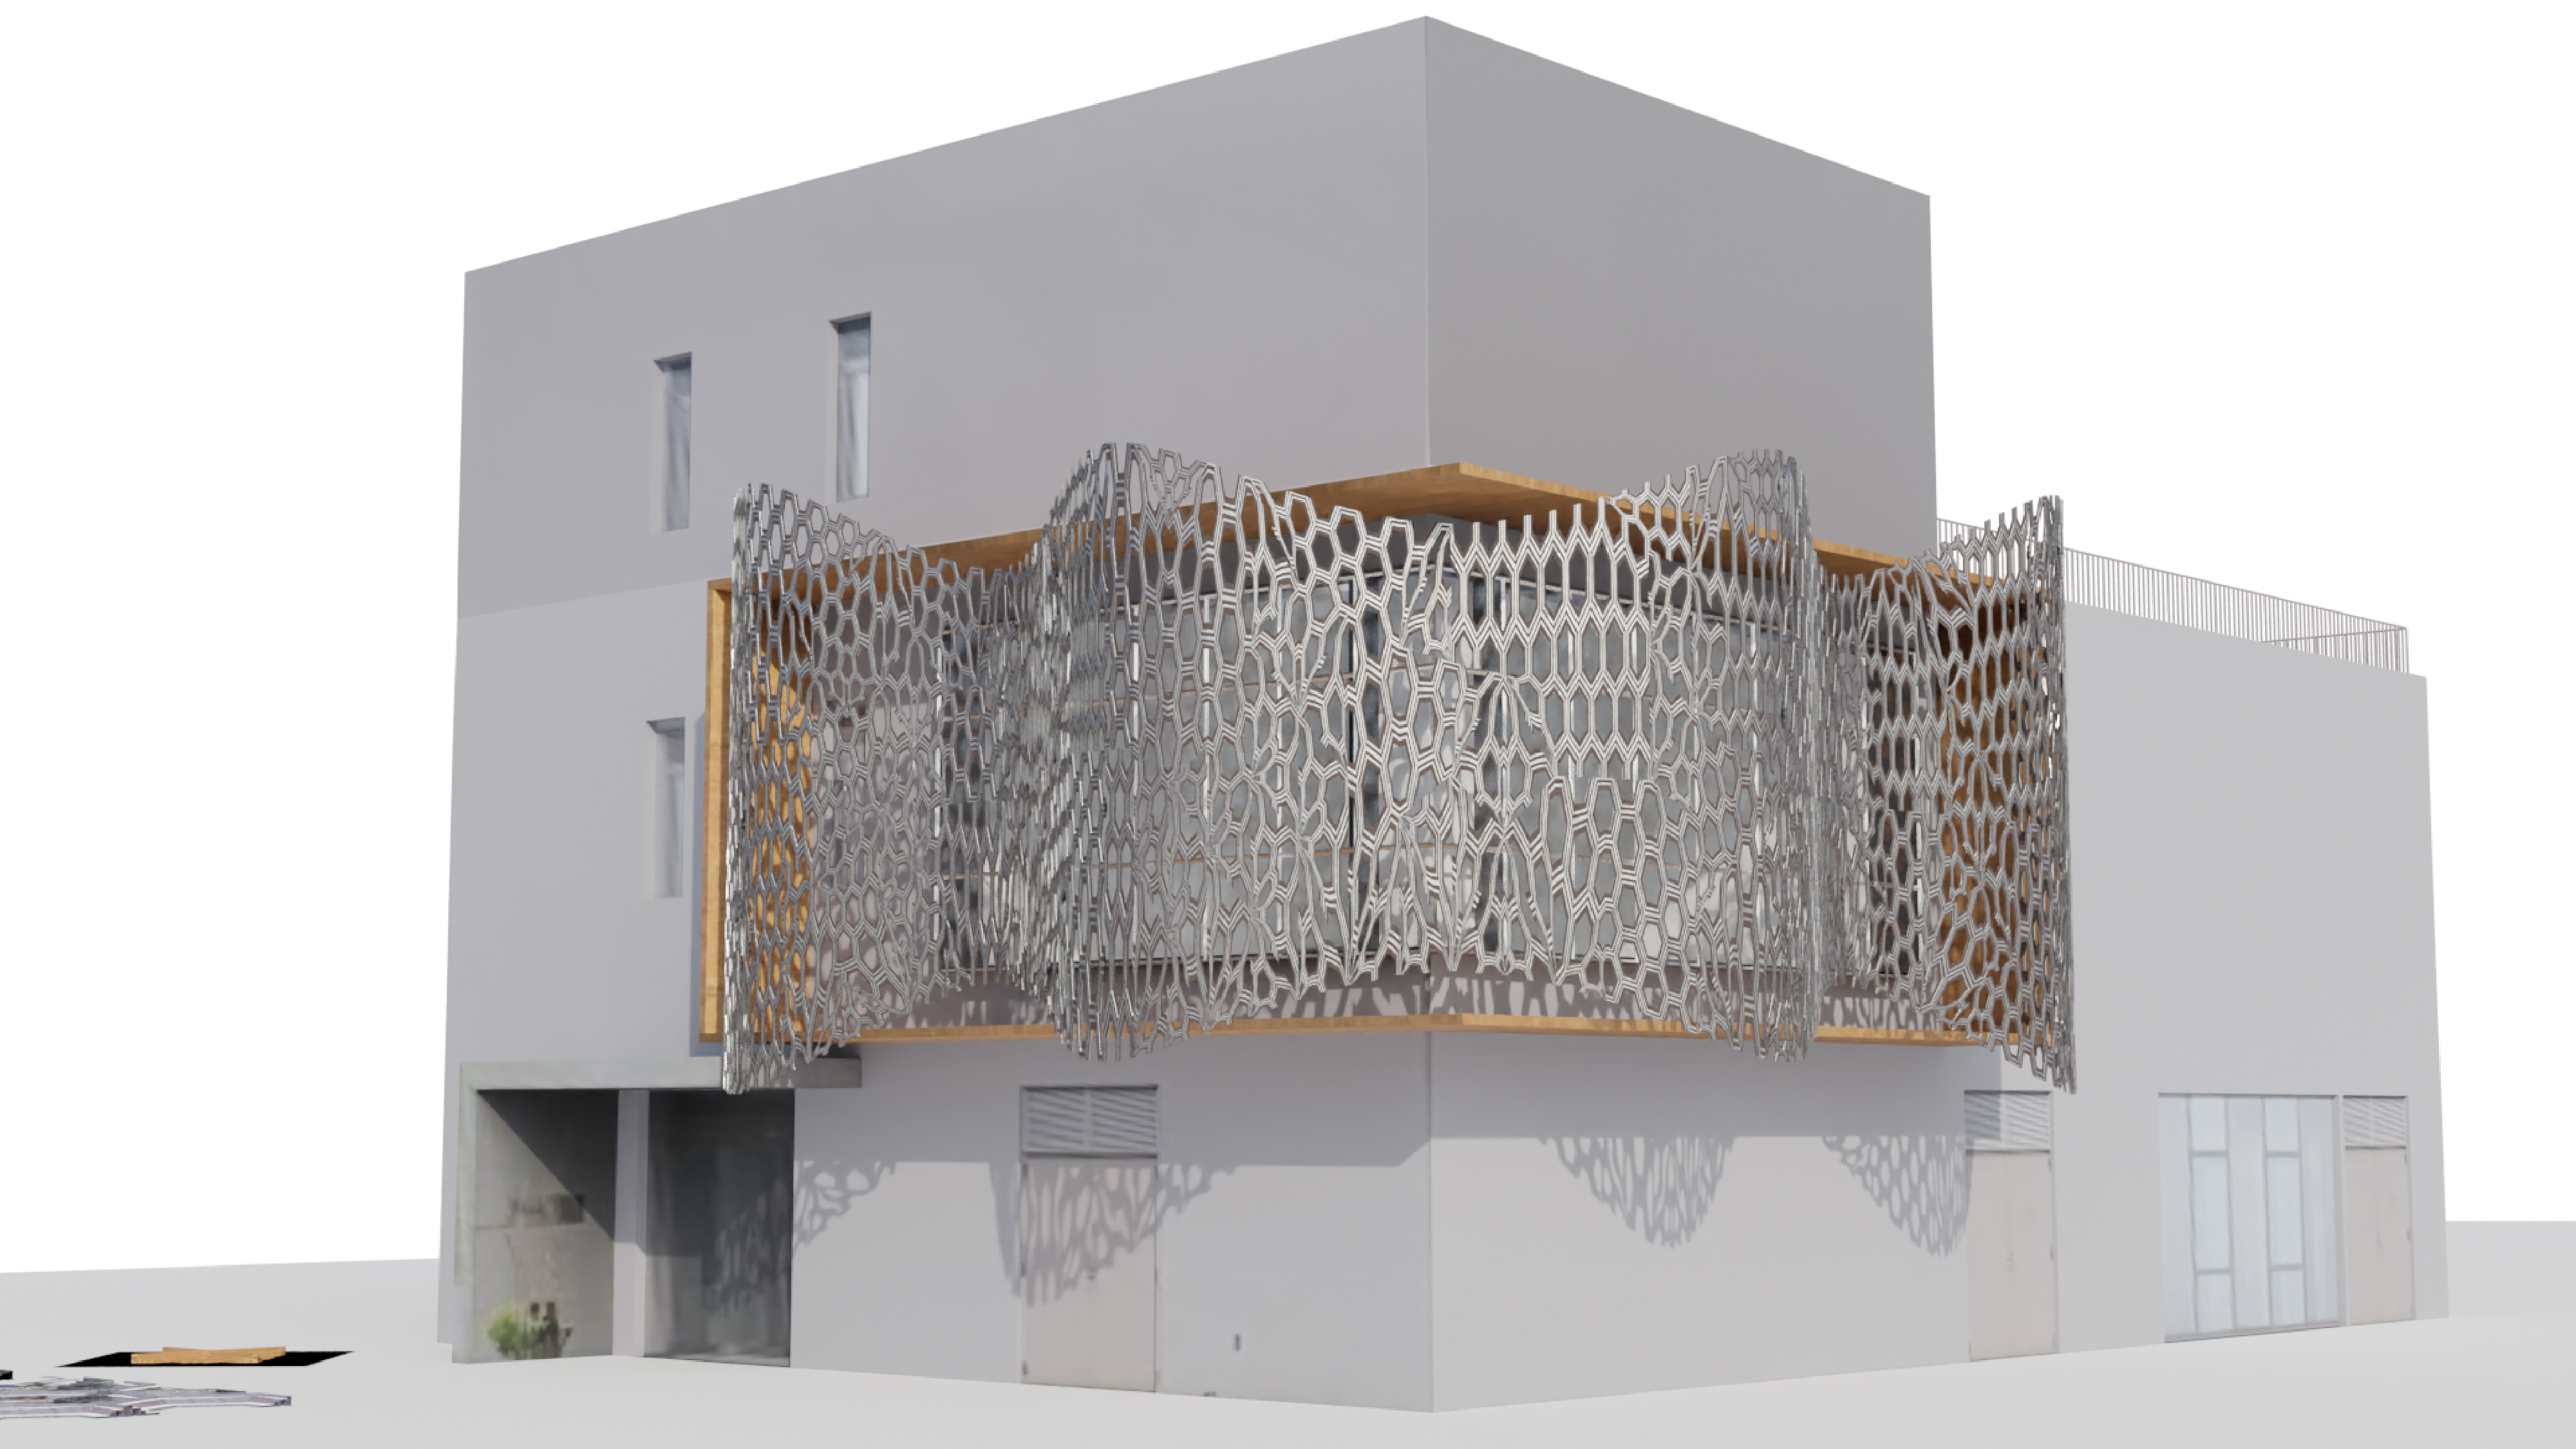
\includegraphics[width=1\linewidth]{Images/Pattern 2/0009}} &
              {\includegraphics[width=1\linewidth]{Images/Pattern 3/0009}} \\
            \bottomrule
        \end{tabularx}
    \end{table*}


    %%Table: Pattern Variations sample 3, 6, 9
    \begin{table*}[htb]
        \centering
        \small
        \caption{Patterns variations for the First five levels of complexity}
        \label{tab:PatternsVariationsPart0}
        \begin{tabularx}
        {\textwidth}{p{4cm} >{\centering\arraybackslash}X >{\centering\arraybackslash}X >{\centering\arraybackslash}X }
            \toprule
            \textit{Description} &
              \textit{Pattern 1} &
              \textit{Pattern 2} &
              \textit{Pattern 3} \\
            \midrule
            \text{Pattern Name} & Hishi Pattern & Tortoise shells & Asanoha Pattern\\

            \midrule
            \textit{Base Module} &  &  &
            \\
            {\includegraphics[width=1\linewidth]{Images/Base Module/Building}} &
              {\includegraphics[width=1\linewidth]{Images/Base Module/Pattern1}} &
              {\includegraphics[width=1\linewidth]{Images/Base Module/Pattern2}} &
              {\includegraphics[width=1\linewidth]{Images/Base Module/Pattern3}} \\

            \midrule
            \textit{Level 3} &  &  &
            \\
            {\includegraphics[width=1\linewidth]{Images/Wall 0/0003}} &
              {\includegraphics[width=1\linewidth]{Images/Pattern 1/0003}} &
              {\includegraphics[width=1\linewidth]{Images/Pattern 2/0003}} &
              {\includegraphics[width=1\linewidth]{Images/Pattern 3/0003}} \\
            \midrule
            \textit{Level 6} &  &  &
            \\
            {\includegraphics[width=1\linewidth]{Images/Wall 0/0006}} &
              {\includegraphics[width=1\linewidth]{Images/Pattern 1/0006}} &
              {\includegraphics[width=1\linewidth]{Images/Pattern 2/0006}} &
              {\includegraphics[width=1\linewidth]{Images/Pattern 3/0006}} \\
            \midrule
            \textit{Level 9} &  &  &
            \\
            {\includegraphics[width=1\linewidth]{Images/Wall 0/0009}} &
              {\includegraphics[width=1\linewidth]{Images/Pattern 1/0009}} &
              {\includegraphics[width=1\linewidth]{Images/Pattern 2/0009}} &
              {\includegraphics[width=1\linewidth]{Images/Pattern 3/0009}} \\
            \bottomrule
        \end{tabularx}
    \end{table*}
